\documentclass{ecsthesis}
%------------------------------------------------------------------------------
\usepackage[english]{babel}
%\usepackage{pdfpages}
\usepackage{natbib}
\usepackage{csvsimple}
\usepackage{longtable} 
\usepackage{wrapfig}
\hypersetup{colorlinks=true,linkcolor=black,citecolor=black}
\usepackage{pdfpages}
%------------------------------------------------------------------------------
\pdfminorversion=5  
\pdfcompresslevel=9 
\pdfobjcompresslevel=3
%------------------------------------------------------------------------------
%% ----------------------------------------------------------------
%% Definitions.tex
%% ---------------------------------------------------------------- 
\newcommand{\BibTeX}{{\rm B\kern-.05em{\sc i\kern-.025em b}\kern-.08em T\kern-.1667em\lower.7ex\hbox{E}\kern-.125emX}}

%% People
\newcounter{address}
\setcounter{address}{1}
\renewcommand{\theaddress}{\textsuperscript{\fnsymbol{address}}}
\newcommand{\address}[1]{\refstepcounter{address}\theaddress#1\\}
\newcommand{\Name}[3]{\texorpdfstring{\href{mailto:#3}{#2}#1}{#2}\xspace}
\newcommand{\SteveRGunn}[1]{\Name{#1}{Steve R. Gunn}{S.R.Gunn@ecs.soton.ac.uk}}

%% Dingbats
\newcommand{\tick}{\ding{51}}
\newcommand{\cross}{\ding{55}}

%% Calculus
\newcommand{\pd}[2]{\ensuremath{\frac{\partial #1}{\partial #2}}\xspace}
\newcommand{\fd}[2]{\ensuremath{\frac{d #1}{d #2}}\xspace}
\newcommand{\dint}{\ensuremath{\int\!\!\!\int}\xspace}
\newcommand{\tint}{\ensuremath{\int\!\!\!\int\!\!\!\int}\xspace}

%% Math Sets
\newcommand{\Q}[1]{\ensuremath{\mathbb{#1}}\xspace}
\newcommand{\R}{\Q{R}}

%% Matrix, Vector
\newcommand{\V}[1]{\ensuremath{\boldsymbol{#1}}\xspace}
\newcommand{\M}[1]{\ensuremath{\boldsymbol{#1}}\xspace}
\newcommand{\0}{\V{0}}
\newcommand{\1}{\V{1}}
\newcommand{\I}{\M{I}}

%% Math Functions
\newcommand{\F}[1]{\ensuremath{\mathrm{#1}}\xspace}
\newcommand{\sgn}{\F{sgn}}
\newcommand{\tr}{\F{trace}}
\newcommand{\diag}{\F{diag}}

%% Math Names
\newcommand{\N}[1]{\ensuremath{\mathit{#1}}\xspace}

%% Data
\newcommand{\mc}[1]{\ensuremath{\mathcal{#1}}\xspace}
\newcommand{\Hyp}{\mc{H}}
\newcommand{\D}{\mc{D}}

%% Kernel
\newcommand{\K}{\M{K}}
\newcommand{\eins}{\texorpdfstring{\ensuremath{\epsilon}}{\textepsilon}-insensitive\xspace}
\newcommand{\e}{\ensuremath{\epsilon}\xspace}
\newcommand{\Bxi}{\ensuremath{\boldsymbol{\xi}}\xspace}
\newcommand{\Kanova}{\ensuremath{\mathit{K_{ANOVA}}}\xspace}
\newcommand{\Kspline}{\ensuremath{\mathit{K_{spline}}}\xspace}

%% Bayesian
\newcommand{\MP}{\ensuremath{\mathit{{\scriptscriptstyle \hspace{-1.5pt}M\hspace{-1.5pt}P}}}\xspace}
\newcommand{\ML}{\ensuremath{\mathit{{\scriptscriptstyle \hspace{-1.5pt}M\hspace{-1.5pt}L}}}\xspace}
\newcommand{\Qw}{\ensuremath{Q_{\w}(\w)}\xspace}
\newcommand{\Qa}{\ensuremath{Q_{\Ba}(\Ba)}\xspace}
\newcommand{\Qb}{\ensuremath{Q_{\beta}(\beta)}\xspace}
\newcommand{\wMPab}{\ensuremath{\w_{\MP|\bar {\Ba},\bar \beta}}\xspace}
\newcommand{\wMP}{\ensuremath{\w_{\MP}}\xspace}
\newcommand{\yMP}{\ensuremath{y_{\MP}}\xspace}
\newcommand{\BaMP}{\ensuremath{\Ba_{\hspace{1pt}\MP}}\xspace}
\newcommand{\aMP}{\ensuremath{\alpha_{\hspace{1pt}\MP}}\xspace}
\newcommand{\bMP}{\ensuremath{\beta_{\hspace{1pt}\MP}}\xspace}
\newcommand{\Sab}{\ensuremath{\M{\Sigma}_{\bar \Ba,\bar \beta}}\xspace}
\newcommand{\Ba}{\ensuremath{\boldsymbol{\alpha}}\xspace}
\newcommand{\Bb}{\ensuremath{\boldsymbol{\beta}}\xspace}
\newcommand{\Bm}{\ensuremath{\boldsymbol{\mu}}\xspace}
\newcommand{\BL}{\ensuremath{\boldsymbol{\Lambda}}\xspace}
\newcommand{\BPhi}{\ensuremath{\boldsymbol{\Phi}}\xspace}
\newcommand{\SMP}{\ensuremath{\M{\Sigma}_{\MP}}\xspace}

\newcommand{\Pa}{\ensuremath{P(\alpha|\mathcal{H})}\xspace}
\newcommand{\Pb}{\ensuremath{P(\beta|\mathcal{H})}\xspace}
\newcommand{\Pab}{\ensuremath{P(\alpha,\beta|\mathcal{H})}\xspace}
\newcommand{\Pw}{\ensuremath{P(\w|\mathcal{H})}\xspace}
\newcommand{\PD}{\ensuremath{P(\D|\mathcal{H})}\xspace}
\newcommand{\PwIa}{\ensuremath{P(\w|\alpha,\mathcal{H})}\xspace}
\newcommand{\PDIwb}{\ensuremath{P(\D|\w,\beta,\mathcal{H})}\xspace}
\newcommand{\PDwab}{\ensuremath{P(\D,\w,\alpha,\beta|\mathcal{H})}\xspace}
\newcommand{\PDIw}{\ensuremath{P(\D|\w,\mathcal{H})}\xspace}
\newcommand{\PwID}{\ensuremath{P(\w|\D,\mathcal{H})}\xspace}
\newcommand{\PwabID}{\ensuremath{P(\w,\alpha,\beta|\D,\mathcal{H})}\xspace}

\newcommand{\PanH}{\ensuremath{P(\alpha)}\xspace}
\newcommand{\PbnH}{\ensuremath{P(\beta)}\xspace}
\newcommand{\PabnH}{\ensuremath{P(\alpha,\beta)}\xspace}
\newcommand{\PwnH}{\ensuremath{P(\w)}\xspace}
\newcommand{\PDnH}{\ensuremath{P(\D)}\xspace}
\newcommand{\PwIanH}{\ensuremath{P(\w|\alpha)}\xspace}
\newcommand{\PDIwbnH}{\ensuremath{P(\D|\w,\beta)}\xspace}
\newcommand{\PDwabnH}{\ensuremath{P(\D,\w,\Ba,\beta)}\xspace}
\newcommand{\PDIwnH}{\ensuremath{P(\D|\w)}\xspace}
\newcommand{\PwIDnH}{\ensuremath{P(\w|\D)}\xspace}
\newcommand{\PwabIDnH}{\ensuremath{P(\w,\alpha,\beta|\D)}\xspace}

\newcommand{\PDwBab}{\ensuremath{P(\D,\w,\Ba,\beta|\mathcal{H})}\xspace}
\newcommand{\PwIBa}{\ensuremath{P(\w|\Ba,\mathcal{H})}\xspace}
\newcommand{\PBab}{\ensuremath{P(\Ba,\beta|\mathcal{H})}\xspace}
\newcommand{\PwBabID}{\ensuremath{P(\w,\Ba,\beta|\D,\mathcal{H})}\xspace}

\newcommand{\PBanH}{\ensuremath{P(\Ba)}\xspace}
\newcommand{\PwIBanH}{\ensuremath{P(\w|\Ba)}\xspace}

%% Snakes
\newcommand{\Esnake}{\ensuremath{\mathit{E_{snake}}}\xspace}
\newcommand{\Eimage}{\ensuremath{\mathit{E_{image}}}\xspace}
\newcommand{\Econt}{\ensuremath{\mathit{E_{cont}}}\xspace}
\newcommand{\Ecurv}{\ensuremath{\mathit{E_{curv}}}\xspace}
\newcommand{\Eint}{\ensuremath{\mathit{E_{int}}}\xspace}
\newcommand{\Eext}{\ensuremath{\mathit{E_{ext}}}\xspace}
\newcommand{\Eterm}{\ensuremath{\mathit{E_{term}}}\xspace}
\newcommand{\Eline}{\ensuremath{\mathit{E_{line}}}\xspace}
\newcommand{\Eedge}{\ensuremath{\mathit{E_{edge}}}\xspace}
\newcommand{\Econ}{\ensuremath{\mathit{E_{con}}}\xspace}
\newcommand{\Eangle}{\ensuremath{\mathit{E_{angle}}}\xspace}
\newcommand{\Elshape}{\ensuremath{\mathit{E_{lshape}}}\xspace}
\newcommand{\Eedgedir}{\ensuremath{\mathit{E_{edgedir}}}\xspace}
\newcommand{\Emodel}{\ensuremath{\mathit{E_{model}}}\xspace}
\newcommand{\wte}{\ensuremath{\mathit{w_{term}}}\xspace}
\newcommand{\wli}{\ensuremath{\mathit{w_{line}}}\xspace}
\newcommand{\wed}{\ensuremath{\mathit{w_{edge}}}\xspace}
\newcommand{\wco}{\ensuremath{\mathit{w_{con}}}\xspace}

%% Environments
\newcounter{alg}
\newenvironment{algorithm}[1]
{
    \stepcounter{alg}
    \begin{table}[htb]
    \centering
    \begin{tabular}[t]{ll}
    \hline&\\
    \multicolumn{2}{l}{\bf Algorithm \arabic{alg}: #1}\\&\\
} {
    &\\
    \hline
    \end{tabular}
    \end{table}
}
        
\begin{document}
\frontmatter
\title      {Method and Theory of Archaeological Spatio-temporal Analysis}
\authors    {\texorpdfstring
             {\href{mailto:Doug.Cowie@soton.ac.uk}{Douglas James Cowie}}
             {Douglas James Cowie}
            }
\addresses  {\groupname\\\deptname\\\univname}
\date       {\today}
\subject    {}
\keywords   {}
\doi {10.5258/SOTON/T0004}
\orcid {0000-0003-1995-2135}
\maketitle
\begin{abstract}
\begin{singlespacing}
Much has been written about spatial analysis, temporal analysis and spatio-temporal analysis of archaeological material. The methods and theories of spatial analysis are a well trodden path, with considerable literature. The methods and theories of temporal analysis are less copious, although there is still a not insignificant quantity of research, weighted slightly more toward the theory than the method. Spatio-temporal analysis can not stake a claim in both of these traditions, it is not the union, but the intersection. Such analysis is required to consider both the spatial and the temporal dimension of the material being analysed.

This thesis evaluates the status quo of the methods and theories of spatio-temporal analysis. It examines current approaches to spatio-temporal analysis through the essential components of theory, method and tools. Following this are two case studies, of very different scales of data set and  analysis, drawing on different intellectual traditions within archaeology. 

The first study, of Hambledon Hill, demonstrates the application of spatio-temporal analysis to a single site, by enhancing the bayesian modelling of the dates. The second study, of the spread of the Neolithic across central and western Europe, takes a continental scale data set and suggests new spatio-temporal methods of analysis.

All archaeological data, sites and processes operate over both space and time, it is therefore inherently a spatio-temporal discipline. Only through combined analysis can such resources be fully analysed, their full potential to tell us about the past revealed. This thesis identifies the complexities and limitations with current approaches for such combined analysis. It offers instead extensions to existing methods and novel forms of spatio-temporal analysis. It demonstrates that such analysis is equally applicable to small and large scale studies and is not the preserve of individual intellectual traditions.

This thesis is about getting the most out of archaeological data. 
\end{singlespacing}
\end{abstract}
%------------------------------------------------------------------------------
% Table of Contents
\tableofcontents
\listoffigures 
\listoftables
\includepdf[offset=70 -75]{decl}
\acknowledgements{Thank you to David Wheatley for your help, advice and most importantly supervision. For seeing nascent potential and patiently drawing it out.

Thank you to Joshua Pollard and Alistair Pike for your advise and recommendations.

Thank you to Alex Bayliss for access to the OxCal project for Hambledon Hill.

Finally, but not least, thank you to my family. In particular my wife Claire for all your support and patience. Also my children Sophia and Miles for the motivation to finish the project.}
\mainmatter
%% ----------------------------------------------------------------
\chapter{Introduction} %5523
\label{ch:intro}
The discipline of archaeology analyses the traces left by people in the past, traces left in both space and time. While the study of spatial data in archaeology is a long one with a considerable literature, the study of temporal data might be considered the poor relation. In fact \citet{Lucas:2005fk} states that a ``proper examination of the concept of time in relation to archaeological theory and method did not really begin until the late 1970s and 1980s'' \citep[28]{Lucas:2005fk}. This situation is now changing e.g. \citet{Bailey:2007fk, CAJ:676016, Bolender:2010po, eps376489} etc. and there is now a wide front on which to engage with time. 

\citet{Lucas:2005fk} divides divides this front along the lines of \citet{Leone:1978fk} and \citet{Bailey:1981uq, Bailey:1983kx}, into archaeologists' perception of time, and past societies' perception of time. With regard to the former a significant amount of work has been undertaken on the use of mathematical techniques to refine dates, in particular radiocarbon dates. A key element of this is known as bayesian modelling, due to its use of bayesian statistical techniques, stemming from \citet{Bayes:1763fk}. The method as used by archaeologists can be traced back to \citet{Buck:1991fk} and see \citet{Buck:1996oq,Buck:2004uq} for more detailed descriptions of the technique. With regard to past societies' perception of time, there has also been the development of a considerable body of literature, for example \citet{Bradley:2002fk}.

This thesis evaluates the state of the art of spatio-temporal method and theory. It will examine how archaeologists deal with time, in particular, how to handle and analyse spatio-temporal data and how it is represented and reproduced. Fundamentally, it will question whether modern temporal techniques lack a consideration of the spatial context, what the negative consequences of this might be, and how space and time may be re-combined.

In order to contextualise this investigation with a site that has been intensively studied, consider Hambledon Hill. Hambledon Hill is a site that will be returned to throughout this study, making particular use of the detailed volume of \citet{Mercer:2008fk}. Very briefly, Hambledon Hill is a site of intense Neolithic activity, including causewayed enclosures, long barrows and defensive earthworks \citep[xiii]{Mercer:2008fk} in South West England. Between 1974 and 1986 Roger Mercer directed a programme of excavation the result of which is the published volume, \citet{Mercer:2008fk}.

The long program of research at the site has created a vast amount of data, but with regard to the temporal data, this falls into several general categories. The field survey \citep[15]{Mercer:2008fk} reports time as the relationship between features, (i.e. earlier/later) while the excavation \citep[41]{Mercer:2008fk} deals with time as probabilistic dates (from radiocarbon determinations) and in relative terms from the stratigraphy. While this last form of temporal data is similar in some ways to the relationships between features in the field survey, it is operating on a different scale. The stratigraphic relationships are also routinely grouped, for example finds and contexts grouped into phases, and in addition there is the difference that phases are referred to by numbers, so there is an inherent ordering. 

Broadly, then, this is in line with the ontology of relative and absolute time, or abstract and substantive time \citep{Lucas:2005fk}. However, it is worth considering if this has to be the case. As Lucas points out, this distinction is perhaps misguided \citep[93]{Lucas:2005fk} as our abstract or absolute time is often loaded with meaning. We must remain aware that our abstract dates also carry subjective connotations for us. Pragmatically however, the types of data that we are dealing with are very different. What one might term absolute dates are of a more numerical form, where as relative dates are a relationship. The absolute, relative division of time is valuable to note the distinction in data, but clearly less so in terms of chronotypes \citep{Lucas:2005fk}.

These two different types of temporal data are used in different, often complementary ways. At Hambledon the relative information from the field survey was used to piece together an idea of the ordering of the use and re-use of the site, for example, this temporal information is used to conclude that a field system pre-dates a Neolithic earthwork, as the field alignment does not follow the earthwork axis \citep[29]{Mercer:2008fk}. However, relative information from the section of an excavation is used to counter this argument, as it demonstrated levelling of banks, and plough soil over the ditches \citep[29]{Mercer:2008fk}. The relative temporal information from the excavation is used to order phases, often given a period, such as Neolithic or fourth millennium BC e.g. \citet[44]{Mercer:2008fk}. They are also associated with artefacts, which can sometimes be dated using an absolute method.

At Hambledon many artefacts were radiocarbon dated, these dates are then used to provide an additional temporal dimension to the phases, based on the abstract radiocarbon scale, or calibrated to calendar years (another abstract representation of time). Such dates are taken from samples throughout the phases and contexts, being used to tie these entities into the abstract chronology of our temporal system. As the authors note, the dates provided by this technique are of the sample (rather than the whole phase) and ``it is the dates of the archaeological events represented by those samples that are significant'' \citep[378]{Mercer:2008fk}. However this presents a problem, the event itself may have been a short lived event, it may have only taken minutes to occur, but the imprecision of radiocarbon dating is such that there may only be an accuracy of a hundred years or so. In addition, there will also be some uncertainty attached to the date, often reported as a confidence percentage, which is due ultimately to the measurement error. These two factors combined mean that the result of such analysis is temporal data of events with a very coarse grained resolution.

If there is a relative chronological ordering between samples and phases, the uncertainty over when within the time period an event actually occurred is not such an issue, therefore the accuracy of the date is less crucial. When there is not any ordering however, being able to refer to the abstract time scale is very useful, as with accurate enough dates it is possible to create an ordering. Using bayesian methods it is possible to combine the radiocarbon and the chronological data to calculate more precise absolute dates, \citep[e.g.][]{Buck:1991kx, Buck:1992ys, Buck:2004uq} which can enable an examination in terms of life spans and generations \citep{CAJ:676016}. Clearly, this makes the ordering and comparison of the dated events much more feasible, and in many ways the focus on the event re-enforces Lucas's argument of breaking down the distinction between the different chronotypes \citep[94]{Lucas:2005fk} mentioned earlier.

Both the bayesian modelling and the using of relative temporal information for ordering are a form of analysis of the temporal data. The absolute dates are used for further temporal analysis at Hambledon, such as developing a sequence for the whole complex e.g. \citet[404]{Mercer:2008fk}, or for determining contemporaneity or clusters of dates \citep[e.g.][405]{Mercer:2008fk} and for putting these into the time scale of peoples' lives. 

Collecting and analysing temporal data is one thing, representing it is quite another. For the Hambledon report a variety of techniques were employed. Radiocarbon dates are most often represented as a date range with a confidence rating as a percentage, e.g. 3680-3620 cal B.C. (68\%) or as a date with standard deviation, e.g. 4870$\pm$45 BP. The former style is often used to represent the date following the application of the radiocarbon calibration process. The bayesian model itself is represented using the OxCal \citep{Ramsey:1995ve, Ramsey:2001zr} output format, which contains the chronological model and absolute dates.

\begin{figure}
\centering
	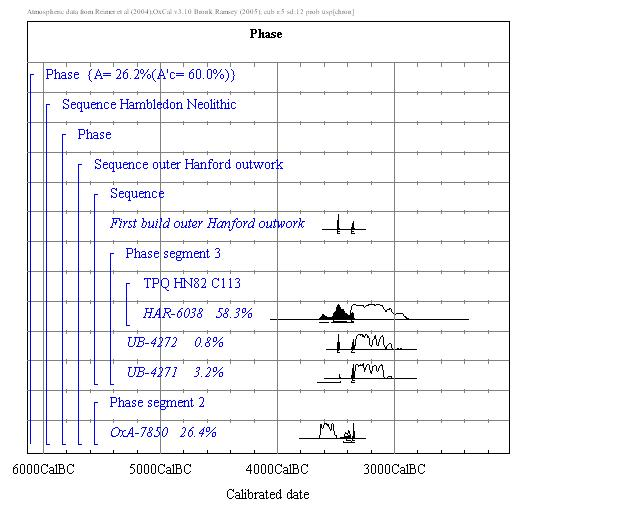
\includegraphics[width=0.9\textwidth]{figures/hanford-remodelled}
  \caption{Example OxCal output, from Hambledon Hill}
  \label{fig:hambledon-oxcal}
\end{figure}

This type of diagram is often used for the visual examination of the dates (see figure~\ref{fig:hambledon-oxcal} for an example) and is clearly completely aspatial. More generally, time is often referenced by specific period labels, as a series of successive snapshots, whose spatial features are then described, e.g. \citet[404]{Mercer:2008fk}. This is a very bland form of representation, simply listing phases by date does nothing to unravel the potential complexities of the temporality of the site. The snapshot representation could be enhanced, for example, by complementing with a more narrative approach, so emphasising the continual nature of change and the development of the site.

The snapshot model is entwined with the phasing of the site, it is well represented by a diagram taken from the report, reproduced in figure~\ref{fig:hambledon-earthworks}. This diagram demonstrates how the earthworks were built up during several phases of use, with each phase being presented as distinctly clear cut, with no representation of duration, or how long it took the changes enacted in each phase to be completed. There is also no clear connection between this plan and the bayesian model, the source of the date values.

\begin{figure}
\centering
	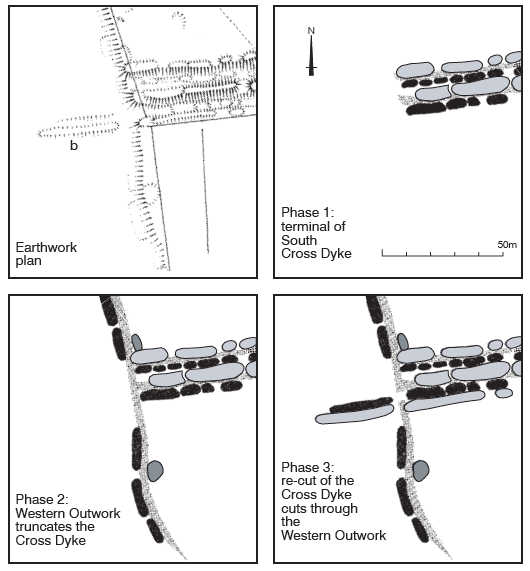
\includegraphics[width=0.9\textwidth,height=0.9\textheight,keepaspectratio=true]{figures/hambledon-earthworks2}
  \caption{Phasing of South Cross Syke, from \citet{Mercer:2008fk}}
  \label{fig:hambledon-earthworks}
\end{figure}

In many ways figure~\ref{fig:hambledon-devel} is similar, however it also demonstrates duration, by specifically identifying already existing features from the previous diagrams in the series, as well as the new ones for a particular phase. This is very similar to an example by Lucas, who suggests that as well as duration such a diagram allows the possibility of multiple phases existing at the same time, which in turn can be used to try and understand the experience of change \citep[41]{Lucas:2005fk}.

\begin{figure}
\centering
	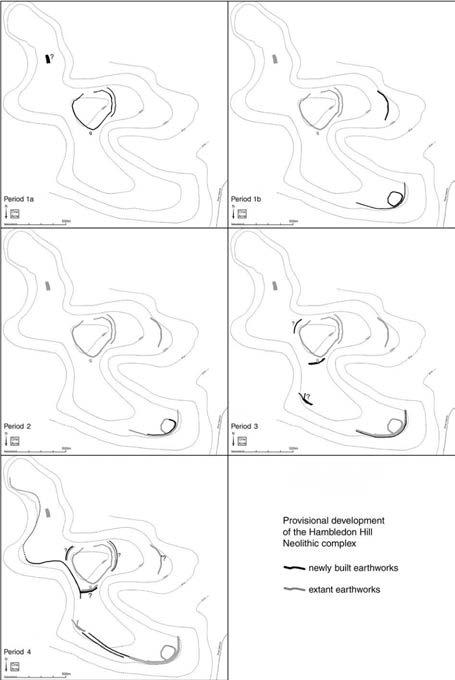
\includegraphics[width=0.9\textwidth,height=0.9\textheight,keepaspectratio=true]{figures/hambledon-devel}
  \caption{Development of Hambledon Hill from \citet{Mercer:2008fk}}
  \label{fig:hambledon-devel}
\end{figure}

These diagrams represent both space and time, which is a bit of a novelty in the Hambledon report and in archaeology more generally. In the reports chapter four, Interpreting Chronology, which covers the bayesian modelling of the radiocarbon dates and where most of the temporal analysis is documented, there are no plan diagrams. It is to all intents and purposes an a-spatial chapter. This is in contrast to chapter three, the excavation, which is in many respects a-temporal, where little chronology is provided, only a few section diagrams. From a narrative perspective, it would surely be inconceivable to divide space and time like this, both are a part of the same whole and complimentary to the story of the site. By separating space and time, it becomes more difficult to consider the continual nature (in time and space) of the processes of change, instead regarding change as the punctuation between specified snapshots.

While the benefits of applying bayesian modelling to individual sites, such as Hambledon, is obvious, they are clearly of limited value to wider questions. A series of studies have applied this method to multiple sites, providing the same benefits to the individual sites, but have also sought to address broader topics using this greater resolution of dating evidence. The original `Histories of the Dead' long barrow project \citep{CAJ:676016,CAJ:676116,CAJ:676124,CAJ:676132,CAJ:676140,CAJ:676148} uses bayesian modelling of radiocarbon dates to create finer chronologies for a group of long barrows, the results of which are then used to re-interpret the early Neolithic of southern Britain. The project was a precursor to `Gathering Time', \citep{Whittle:2011kl,Whittle:2011tg} a much larger project, focussing on 40 Neolithic enclosures in southern Britain, including Hambledon Hill, culminating in a re-appraisal of the temporal evidence for the early Neolithic in Britain. More recently `The Times of Their Lives' \citep{whittle2018times} applies these techniques to a large number of sites spread across continental Europe to address a range of theoretical issues. In these studies each site had its own specific research questions, the bayesian technique has helped answer these, in addition there were also overarching questions about the early Neolithic, such as ``When did causewayed enclosures begin to be built in Britain and Ireland'' \citep[13]{Whittle:2011kl}. 

For each of the individual site studies, there is often very limited spatial information. As an example, Hill Croft Field \cite[521]{Whittle:2011tg} contains no plan of the site at all. Between both Times of their Lives and Gathering Time, only one site has more than one plan, Fussells Lodge Long Barrow, in \citet{CAJ:676132} and they are rarely referred to. 

The data for both the radiocarbon determinations and the chronology at first glance appear distinctly absolute and un-problematic for input to a digital system. The radiocarbon being a probability distribution, and the chronology stored as a graph or tree type structure of nodes and relationships. Unfortunately, this line of reasoning leads straight into a trap; in many case studies, multiple models are given for each site because the models are based on an interpretation, there is no single version of the truth, only potential scenarios. If one were to simply take the preferred model and store it as `the' chronology for the site, this is taking something, which has an associated probability, and making it absolute and concrete. This is discussed in \citet{CAJ:676108} with reference to the quote on models often attributed to George Box - ``All models are wrong, some models are useful'' along with several techniques for determining the validity of different models. However, while it would be preferable to have certainty or quantified uncertainty, this is not always possible or ideal when dealing with multiple potential interpretations. Instead \citet{CAJ:676108} take a multiple pasts approach where the ``production of alternative models, none of them definitive, is simply a means of creating multiple pasts and is entirely congruent with the post-modern perspective'' \citep[5]{CAJ:676108}. The issues of exactness and the authority of computer generated results is clearly a crucial problem, as \citet[201]{Ramsey:2000fk} notes: \begin{quote}``there is no one correct prior for a given situation. A prior is merely a model that can be applied to the data to help in its interpretation. Ideally, several different models with different priors should be tried \ldots this approach may not appeal to some people who wish to take their results, process them statistically and come out with the `right'�� answer''.\end{quote} A pertinent quote to match that by George Box is one commonly attributed to John Tukey ``An approximate answer to the right problem is worth a good deal more than an exact answer to an approximate problem''.

Each of the individual studies has its own objectives, these objectives dictate the specific methods of analysis performed using the temporal data. The objectives are typically concerned with dating phases of construction and the duration of use, e.g. \citet[80]{Whittle:2011kl}. In addition, the results are combined to answer some more general questions about the British Neolithic, \citep[13]{Whittle:2011kl}, or to suggest connections between areas considered in the study, \citep[432]{Whittle:2011kl} and to challenge some specific theories or ideas, such as the connection between the continental LBK longhouses and British long barrows \citep[139]{CAJ:676156}. To answer these questions the primary form of analysis that has taken place is the bayesian technique, which combines the models and radiocarbon dates to create refined dates. This is also used to create the multiple pasts referred to above, based on the variations in the chronological model. Using the refined dates, further analysis is performed to examine durations, such as the number of years different part of a site were used for e.g. \citet[91]{Whittle:2011kl}. 

The topic of bayesian modelling of dates is not without controversy. In a recent review of the literature \citet{doi:10.1080/00438243.2015.1070082} split the main issues into ``whether the assumptions that underlie bayesian models are justifiable; and whether ��prior�� information essential to their construction (in this case, samples that have been dated) is relevant and reliable.'' \citep[527]{doi:10.1080/00438243.2015.1070082}. A large part of the study of each site is spent in justifying the inclusion or exclusion of samples (as recommended by \citealp{doi:10.1080/00438243.2015.1067640}) with any area of contention leading to the creation of multiple models, discussed in additional detail. The assumptions that underpin the model are generally presented textually, although in some studies stratigraphic relationships between samples are shown graphically, e.g. \citet[92]{CAJ:676140}. While such models as e.g. \citet[49]{CAJ:676124} are more stylised, in some publications the chronology presented to justify the bayesian model is similar to Harris-Matrix diagrams (e.g. \citealp[167]{AQY:9543450}). Clearly the validity of the model underpins any subsequent analysis performed on the results, it is therefore imperative to make sure such models are built on solid foundations. The problem is how to do this, \citet{doi:10.1080/00438243.2015.1070082} suggest that all models must be open to scrutiny \citep[14]{doi:10.1080/00438243.2015.1070082} which is clearly important for independent validation of results, and they also note it is important to select samples pertinent to the archaeological question \cite[4]{doi:10.1080/00438243.2015.1070082}. In this, Gathering Time is successful, their models and reasoning are published, although I am not aware of any independent validation of the results.

The next step is to consider how these projects represent time, including the results of the analysis. A large part of each study is devoted to a textual description of each of the samples and of the chronological model, with diagrams of the OxCal models, similar to those from Hambledon. Additional analysis such as durations are presented in a similar diagram generated by OxCal, the results from these diagrams are then used directly to answer the objectives of the studies. The multiple, alternative models are presented independently, with the preferred model being described in most detail, and other models gone through in a similar fashion, with particular focus on the areas that are different. This is a perfectly reasonable approach, although a graphical side-by-side representation would highlight the differences, and perhaps re-enforce the multiple realities aspect of multiple chronological models.

In the textual description of the temporal data, the authors convert their dates to life spans and generations, with life spans being set at 70 years, and generations set at 25 years \citep[16]{Whittle:2011kl}. These measures of time are then used to translate the output of the bayesian modelling into a format of date that has a more immediate human resonance, e.g. \cite[132]{CAJ:676156}. While this humanising of otherwise dry data is a welcome attempt at going from abstract chronologies to a more personal time scale, it is highly interpretative, not only the underlying dates, which are probabilities, and could easily not fit the neat small time spans of generations or life spans, but also the figures chosen to represent life spans and generations. Clearly, this is a what-if, an invite to picture how the monuments might resonate to a human time scale. In many ways, this type of interpretation is as much a form of representation of the temporal data as the graphical diagrams and models. It has been used successfully in other studies, 
\cite[e.g.][654]{doi:10.1080/00438243.2015.1053976} to contrast the prevailing view of conservatism with the dynamism implied by the results.

This representation is almost entirely a-spatial, a uni-dimensional representation of otherwise rich data, the reader could refer back to the (often) single plan, but this is not really enough, such a dimensionality reduction makes it much more difficult to analyse the changes or processes being included in the model. By leaving out the spatial data almost entirely it is difficult for the reader to become engaged in the analysis, the authors clearly known the proximity of the dates, but to anyone else they could all be at the exact same spot. Leaving out the spatial data makes it also nearly impossible to judge the scale of the site or sites being discussed. This is not uncommon in the bayesian literature,  \citet{doi:10.1080/00438243.2015.1053976} for example, only contains a map of Great Britain highlighting sites mentioned in the text, despite discussing in detail different parts of a key site. Combining time and space into a single diagram is difficult, but not a new problem \citet{Johnson:1999cr} mentions four methods often used by cartographers to include a representation of time in their diagrams, (see figure~\ref{fig:time-maps}) these being time slices, symbolism, arrows and difference maps. He refers to these methods as ``squeezing extra dimensions'' \citep[27]{Johnson:1999cr} out of two dimensional representations, and argues that they do not do justice to the underlying data, instead he recommends animation as it is a form or representation which makes use of time itself \citep[28]{Johnson:1999cr}.

\begin{figure}
\centering
	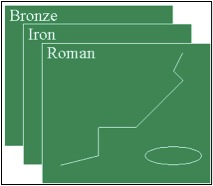
\includegraphics[width=0.4\textwidth]{figures/time-slices}
	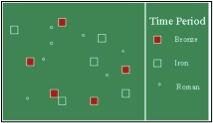
\includegraphics[width=0.4\textwidth]{figures/time-symbol}
	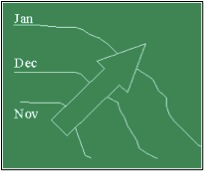
\includegraphics[width=0.4\textwidth]{figures/time-arrows}
	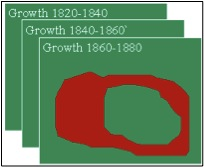
\includegraphics[width=0.4\textwidth]{figures/time-diff}
  \caption{Traditional methods of cartographic representation: a. Time slices; b. Symbolism; c. Arrows; d. Difference maps, from \citet{Johnson:1999cr}}
  \label{fig:time-maps}
\end{figure}

More recently \citet[7]{lock2002analysing} suggested a 3D method which would also permit the uncertainty of dates to be displayed as part of the diagram, by including a 3rd axis (in additional to two spatial) where the less likely a site is of being in use, the less clearly it is drawn (for example dashed or dotted lines for features are used instead of uninterrupted ones). Both of these proposals have serious issues, which will be examined in more detail later on in this study, for now let us briefly consider them. Animation as a form of representation might be suited to showing objects or events with certain dates, but once these dates become probabilistic, it will soon become an unclear mess of many objects or events. These events may or may not even have occurred simultaneously, potentially creating a false sense of synchronicity between events, which in fact did not occur at the same time. A similar problem exists with representing the probability of use as a third axis, in this case it will be easier to see that events may not be concurrent. But with more than a few dates, especially with overlapping spatial data, the diagram will rapidly become unreadable. That none of these techniques has been used in practice to include a representation of time with spatial data is a shame, as experimentation can lead to innovation, but it also suggests that the problem is perhaps a tricky one, and that a bit of cartographic magic will not do full justice to the underling data.

In some respects there are parallels with what \citet{Rennell2012} has termed subject-centred landscape archaeology. In such studies, diagrams often take a back seat role, compared to the detailed textual description. An example of this is \citet{Vavouranakis:2006fk} which features a descriptive study of the landscapes of the town of Gournia, a ``series of meaningfully constructed landscapes, ranging from the personal, familiar, and mundane to the economic, political, ritual, and exceptional'' \citep[237]{Vavouranakis:2006fk} and of how these landscapes developed over time. It focused on how societal changes may be being reflected in changes to buildings, presented in a broad narrative, with only a couple of maps to provide context. By considering change over time, that study was moving towards a more integrated spatio-temporal analysis, but unlike the more exclusively temporal studies mentioned above, it focuses on spatial elements by taking a (spatial) narrative approach to moving through the landscape. Crucially the narratives are presented sequentially, as a textual snapshot based model, one for early, middle and late Bronze Age. There is little consideration for the process of change, only a description of those changes. Clearly this approach would benefit from the addition of a temporal narrative, a description of the interplay between the eras, and of how past, present and future should be just as much the targets of a subject-centred study. While this kind of approach has a lot to offer, I'm not convinced that it would make full use of the refined dates and multiple pasts created by bayesian techniques. Fortunately, \citet{Rennell2012} also demonstrates several techniques for combining methods of subject-centred survey with more traditional spatial analysis, such as comparing visibility on the ground with computed viewsheds, and augmenting continuous viewsheds with details of journeys through the landscape. By combining techniques in this way a more holistic interpretation and analysis is possible, something lacking with current temporal techniques.

The field of spatial analysis has several parallels with the kind of temporal analysis reviewed above, there are different types of data, vector and raster, a range of statistical analysis techniques, and a need for specialist software. A key difference between the two areas is the available methods, where as the spatial analyst has a toolbox of techniques including spatial searches, digital elevation models, clustering, autocorrelation, viewsheds, etc, there is a paucity when it comes to temporal equivalents. Bayesian modelling is clearly a powerful technique, which can be used not only to refine dates, but also to examine chronologies, calculate durations of use, or inactivity. In addition, there are other temporal methods, such as summing radiocarbon dates, or the chi-squared approach to wiggle matching, however, some of these appear to have been in decline in recent years \citep[678]{doi:10.1080/00438243.2015.1067640}. Ultimately these methods are about refining the data, unlike the spatial techniques, which are about highlighting information that is not immediately apparent in the data. The field of temporal analysis is arguably only just beginning to flourish, especially bayesian modelling of dates, where the majority of papers have only been published in the last five years (as of 2015) \citep[678]{doi:10.1080/00438243.2015.1067640}.

Clearly, the archaeological questions asked dictate the analytical methods used, up to now the kinds of questions asked of temporal data are familiar. For example \citet{CAJ:676116} looks to: determine if there is a gap between Mesolithic and Neolithic occupation, and if so for how long; to determine a date and duration for the Neolithic occupation; to see if there was a gap between occupation and barrow construction; to date the contraction of the monument; to determine the duration of infilling of ditches; to date the barrow extension; and to date the burial activity in the cists. These kinds of questions fall into two categories, questions of date and questions of durations. For these kinds of questions, the bayesian methods are clearly appropriate, providing more detailed answers than previous methods. However, these are the same kinds of questions that have been asked of temporal data for a long time. For the field of temporal analysis to expand and flourish, it is crucial to start asking other kinds of questions, which will lead to new forms of analysis. And it will be essential to engage with theoretical questions, a prime (non-temporal) example of this is \citet{Evans:2006fk}, which analysed the identity prescribed to individuals based on grave goods in Iron Age France, specifically notions of gender and social standing. Using the mean frequency of artefacts Evans was able to show that burials with engendering grave goods assemblages were likely to have more goods overall, implying a higher social prestige \citep{Evans:2006fk}. In addition, the statistical analysis was able to demonstrate a change in goods frequencies over time, implying a change in the nature of status and in gender roles. Evans took the statistical results, and linked them to theoretical issues of status, going from descriptive to the interpretative. This is important for temporal analysis, it is already happening, slowly, for example in \citet{CAJ:676156} the issue of the influence of continental long houses on British long barrows is discussed. But more could be done in this area to make this kind of question the ultimate objective, and make the determination of dates just a step down the path.

To recap, there is a burgeoning field of temporal analysis, several example studies with a temporal focus have been examined in detail, and many other studies drawn on. They shared common forms of temporal data, primarily radiocarbon dates and chronology, and common methods of temporal analysis. This analysis is mostly based upon bayesian modelling of dates, which has been used to answer typical questions of age and duration. This technique is not without its problems. While mathematically rigorous it requires interpretation for the construction of chronologies and its graphical outputs are not always straightforward to interpret. It also leads to the creation of multiple models, which may be problematic. Temporal data has generally been presented in a textual, a-spatial format, often accompanied by technical diagrams from bayesian modelling software. This is a clear limitation of current approaches, with the lack of any spatial element going right through the process, all the way back to data collection, where it is treated independently from temporal data. Perhaps this is considering spatiality and temporality as being two sides of the same coin, however we should also surely be considering the coin as a whole. The next step for archaeological temporal analysis is to include the spatial information, so that it becomes spatio-temporal analysis, to unify both sides of the coin. Only by combining the two will it be possible to fully utilise the temporal data available. 

Such analysis is a rare thing in Archaeology, but not wholly unheard of, for example a series of studies have looked at the spatio-temporal patterns of the Lowland Classic Maya collapse \citep{Bove:1981fk,Whitley:1985uq,Kvamme:1990kx}. In the initial study, \citet{Bove:1981fk} constructed several trend surfaces (see figure~\ref{fig:bove-map} for an example) for the dates of the latest stelae (stone monuments) at each settlement. Trend surfaces are usually a tool for spatial analysis, and are a means of fitting a function through a set of values \citep{Bove:1981fk}. In this case, the values are the date of erection of the last stone monuments, with the height of the surface calculated based on these dates, so the spatial trend was a temporal one, showing where the end of construction of these monuments started, and how it spread spatially. Using this technique, Bove was able to argue for a regional approach to the collapse \citep[111]{Bove:1981fk}, with outside groups possibly moving in to exploit a power vacuum \citep[110]{Bove:1981fk}. This analysis was then verified using spatial autocorrelation, firstly by \citet{Whitley:1985uq} who attempted to demonstrate that no simple geographic pattern existed, \citep[390]{Whitley:1985uq} and then later by \citet{Kvamme:1990kx} who showed that such a pattern did exist \citep[203]{Kvamme:1990kx} and that the technique employed in \citet{Whitley:1985uq} was unsuitable for the data \citep[201]{Kvamme:1990kx}. 

\begin{figure}
\centering
	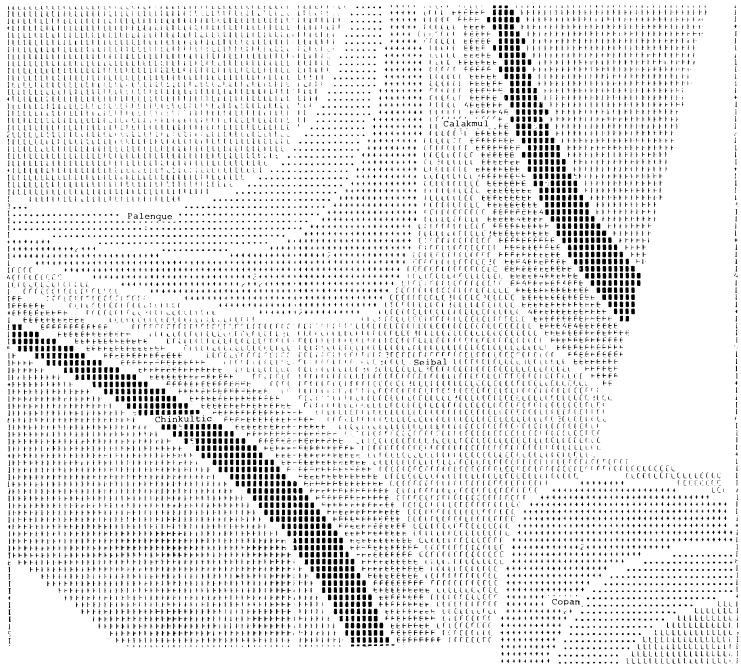
\includegraphics[width=0.9\textwidth]{figures/maya-1}
  \caption{Second-order trend surface contour map, from \citet{Bove:1981fk}}
  \label{fig:bove-map}
\end{figure}

Such interesting analysis would not be possible if space and time had been considered independently, by combining them in this way it has been possible to learn much more about the Lowland Classic Maya collapse. In order to combine both space and time in this case, spatial techniques have been applied using temporal data as an attribute, for the trend surface, a z-axis value. This is a straightforward approach using existing, already tried and tested methods with appropriate spatio-temporal data. The difficulty in performing spatio-temporal analysis like this more broadly is in having temporal data that can be used. Fortunately, there is high-resolution temporal data for the erection dates of the Maya stone monuments that enables these dates to be presented as specific years on our calendar. A lot of archaeological temporal data does not fit into this exact, historical form, being less certain, in many cases probabilistic. In order to easily perform analysis, which is repeatable, and combines both spatial and temporal data we will require the use of specialist methods that can cope with archaeological temporal data and software to perform analytical techniques.

Fortunately within archaeological Geographic Information System (GIS) studies, there is a seam of research into Temporal GIS (TGIS). This would provide software that could operate on spatial data as a GIS does, but could also incorporate temporal data, and perform operations and analysis on combined spatio-temporal data that go beyond treating time as an attribute of spatial data, elevating it to being an equal part of the analytical technique. Such a system would also be capable of comprehending and working with the types of temporal data archaeologists have available. 

This brief overview has toured both method and theory of spatio-temporal analysis at both a small and large scale. It has shown that to gain maximum benefit from spatio-temporal research, the necessity to re-contextualise the temporal data with its corresponding spatial component. The subject has been approached from a temporal perspective, taking the site of Hambledon Hill to understand the full life cycle of temporal data, ultimately, from it's place in the ground, to the regional analysis of Gathering Time. The theories and methods of spatio-temporal analysis are relevant throughout that life cycle. This introduction to the topic has identified three key components in the study of spatio-temporal data, in fact all archaeological data. By examining each of these components in turn, we will not only understand the state of the art of the subject, but will be in a position to enhance the value that can be obtained from the analysis of archaeological data. 
\begin{enumerate}
\item Asking the right questions -
as mentioned above, the questions dictate the methods, therefore it is important to at least start to address them first. In order for the field of temporal analysis to progress, it is crucial to move from descriptive questions to those of a more analytical or interpretative nature. This component will consider what kinds of questions are asked of temporal data, with an aim of enhancing such questioning by an inclusion of the spatial dimension.
\item Analytical techniques -
next, it is necessary to consider what methods are available to analyse the data, the validity and the general acceptance of those methods. We must also consider whether the currently available methods will actually help answer our questions, or if new methods will be required. Finally, it is important to consider the correct application of such methods, as without this how can the validity of any results be ensured?
\item Spatio-temporal software -
specialist software will be required to handle the data and perform the analysis, as current GIS platforms do not handle the probabilistic dates of archaeology. This chapter will review the available options, and determine if any can be used out of the box, or if not, what can be learnt about the most effective way of meeting these technical requirements.
\end{enumerate} %5,525
\chapter{Questions for Spatio-temporal Data} %9430
\label{ch:question}

\section{Current Approaches to Questions}
In order to be able to ask better questions it is necessary to first have an understanding of the limitations of current approach to questioning data. Considering Gathering Time, each of the case studies in the two volumes generally considers basic temporal information such as construction dates. For example, at Windmill Hill an objective of the study was to find the date of construction of the enclosure and its constituent circuits \citep[80]{Whittle:2011kl}. In addition, for Windmill Hill, the study aimed to find the duration of primary use, duration being another question consistently asked throughout the study. These two common types of question come in several forms, the first type, ``what date is x?'' also take the form of ``is x earlier or later than y'' as in order to answer this question the dates of x and y are required, these questions are limited in scope to the date itself. The second type of question is where the primary temporal data is used to create some other value or data, for example, in order to calculate duration it is necessary to first calculate two dates to be able to then determine the duration between them. For both these types of question the focus is on the temporal data, even though for the second type the answer actually comes from some derived data. Finally, there are those questions that engage with some level of archaeological theory. Examples of this type of question would include ``whether the contrast in plan and scale between the inner and outer pairs of circuits indicates diachronic construction'' \citep[219]{Whittle:2011kl}, ``Did the simple stratigraphic sequences at Etton Woodgate and Northborough correspond to shorter use-lives than those reflected in sometimes complex histories of recutting and backfilling at Etton'' \citep[318]{Whittle:2011kl} and ``establish whether any of the dated bones were already old when placed in the monument'' \citep[48]{CAJ:676124}. At first glance such questions seem almost entirely heterogeneous, there is no common format or pattern, they are all fairly specific, asking detailed questions of a site that engage with various theories about the site, and how it was used in the past.

These categories of question are fuzzy and in many ways cumulative, for in order to answer those in the final grouping, we will have to have data that could be used to answer questions of date and duration. The kind of questions examined above are being asked and answered with modern analytical techniques. In many cases the more interesting, theoretical questions do not require a special methodology, they simply require the application of the data from the primary analysis to the task of interpretation. This raises the question of why such questions, that engage with theory, are not asked more routinely?

This is not to suggest that the more rudimentary questions are less important, merely that they are limited in scope. In order to make full use of spatio-temporal data it is necessary to ask questions which really push at the boundaries about what is known of people in the past. These kinds of questions, which engage with archaeological theory, have been described as ones that ``investigate \ldots questions beyond the descriptive''  \citep[51]{Evans:2006fk}. They go beyond simply describing the results of statistical analysis, engaging with a theoretical question, with the ultimate objective of influencing archaeological theory, or to put it another way, re-building the scaffolding required to treat data as evidence \citep{doi:10.1177/0162243916671200}.

What Evans means by this is that we should not be satisfied with the ``how old is x'' kinds of questions, and instead should be focusing on questions that use the data to take us closer to the people being studied. In many respects this is not too far removed from the more narrative speculation often placed at the end of publications, however, these spatio-temporal questions should be being asked more formally and make explicit references to their data. With the finer grained dating evidence now available via bayesian modelling such questions should be supplementing (or replacing) the more mundane ``what date is x'' type questions in the core of research.

Clearly these kinds of questions are already being asked of temporal data. But not frequently enough, and there are few examples of such questions engaging with both spatial and temporal elements of the data. In order to examine kinds of questions that should be being asked of archaeological data, it is necessary to engage with archaeological theory. The following section will examine aspects of temporal theory that could provide inspiration and a framework for asking interesting questions. Temporal theory has been chosen for the focus as all of the temporal concepts could be easily extended to include a spatial component and there is a lack of application of this theory, especially when compared to spatial analysis. This is due to the ready availability of spatial techniques from other fields, which could be applied wholesale to archaeological data. This is in contrast to temporal methods, where techniques from other disciplines are not so applicable and a body of theory has developed without this influence. \citet{Bailey:2007fk} has recognised there is a chicken-and-egg situation here, between temporal analytical techniques and questions to ask, how can one ask questions without knowing what techniques are available? But it is not possible to know what tools are required until the questions have been asked. This thesis will start with the questions, as even if it is not possible to answer them at present, it may become so in the future and because starting with the tools may introduce an unintended bias if they are all developed under the same theoretical framework. 

\section{Temporal Theory}
There are a wide range of different topics that fall under the heading of time in the past, and a variety of authors, taking varied philosophical perspectives have focused on these different topics. In a broad review of the area Lucas splits it into the study of time perception and the study of the temporal structure of past activities, however he argues for a close connection between the two, stating ``Society does not solely perceive time through time-marking systems, but through the very temporality of its practices'' \citet[70]{Lucas:2005fk}. While Lucas acknowledges the study of temporal perception, he sees more benefit in the analysis of temporal structure. The analysis of the temporal structure of activities, or time-consciousness, is broken up by Lucas into social memory and social recollective memory. Where social memory is more near term, within living memory, focused on the reproduction of society. While social recollective memory is concerned with more distant times, the use of ritual to engage with the past \citep[84]{Lucas:2005fk}. This is the focus of \citet{Bradley:2002fk} who splits the temporalities into the distant past, a time concerned with origin myths of a society; the immediate past, which focuses on how people would have been aware of the history of their society; the future,  how monuments were used to shape the memories of the future; and finally how people in the past would have responded to evidence from the past.

Such a perceptual approach to time is criticised by \citet{Bailey:2007fk}, who is concerned that the multiple temporalities studied by Lucas and Bradley are in fact temporalities that exist in our present day society, and that we have no evidence that people in the past had the same awareness of time. In fact, he states ``when archaeologists claim to reveal the subjective experiences of past people, [we have no guarantee] they are doing anything other than imposing their own'' \citep[219]{Bailey:2007fk}. Such an attack appears to cut to the core of the Lucas and Bradley's approach to time consciousness, however it need not be absolutely the case. Take, for example Bradley's idea of the mythical past, this is clearly a subjective temporality we can understand, but Bradley's argument does not necessarily mean that people in the past would have attached the same connotations to the idea of a mythical past that we do today. These are words and phrases to help us understand, and are not necessarily prescriptive of what a mythical past might mean to someone in the past. His argument is perhaps more that the concept of a mythical past is the closest analogy that we have to the temporality he is studying. However, Bailey is making an important point about using our own preconceptions of time to cloud how we view the past, it is somewhat ironic that Lucas is guilty of this, as he attacks chronology for leading to totalizing grand narratives, a modern western view of time \citep[13]{Lucas:2005fk}. 
 
\subsection{Time Perception}
Issues of time perception can be studied directly by looking for evidence of devices used for temporal reckoning, an example of this being the alignment of Neolithic stone monuments in Europe, providing evidence for awareness of periodic events such as the winter solstice \citep[73]{Lucas:2005fk}. While there are clearly potential avenues of research in the field of time perception, it is in some ways quite a limited field of study, the evidence required for a convincing ``proof'' of an awareness of time usually relying on how likely the apparent observance could have occurred by chance. There are also potentially complicated issues of interpretation, for example, solar observances may have a related alignment to other events, such as the midwinter sunset being on the same alignment (but exactly opposite) the midsummer sunrise. Even with clear evidence for an awareness of such events, it is essential to consider the distinction made by Lucas and others between time reckoning and time indication \citep[68]{Lucas:2005fk}. While this is evidence for the reckoning of time, it does not imply some sort of calendar, or system of measuring required for time indication. Presumably, any society that relies on horticulture would have to be aware of the changing seasons in one way or another, for the yearly planting of seeds, harvesting, etc, but they would not necessarily record their passing. It is perhaps this type of ambiguity which leads Lucas to the conclusion ``��it is really when archaeology leaves the realm of trying to recover evidence of time-reckoning and explores more general issues of temporal perception in the past and its relation to social practice that the most rewarding studies are to be found''�� \citep[77]{Lucas:2005fk}. 
 
\subsection{Temporal Society}
There is evidence for the temporal structure of past activities, or time-consciousness, in a range of practices. Lucas defines the concept of social memory as the transmission of knowledge in non-literate societies, \citep[77]{Lucas:2005fk}. He argues that the reproduction of society is largely dependent on repetitive incorporation practices. In addition, where such practices are evident in the archaeological record he states they will convey something of the nature of social memory and cultural transmission simply because they tend to be repetitive and incorporative \citep[78]{Lucas:2005fk}. This is down to the innate temporality of society, as recognised by Bradley, who stated ``Time is part of the process of living in society'' \citep[5]{Bradley:2002fk}. Bradley defines two possible methods for the acquisition of social memory, firstly it might have happened by bodily practices including participations in rituals, ceremonies, social conventions, correct behaviour and appropriate use (and destruction) of material culture \citep[12]{Bradley:2002fk}. Secondly, by the building of monuments designed to perpetuate a particular worldview \citep[12]{Bradley:2002fk}. For Lucas, social memory is studied by the explicit analysis of continuity or repetition of cultural practice over a long period, by examining the nature of the practice and what it implies in terms of social memory, \citep[82]{Lucas:2005fk} this being broadly in line with Bradley's bodily practices.

Closely linked to this is the study of continuity (through social memory) or the lack of it. It could suggest conservatism as opposed to innovation, in this case, it would be valid to ask what is the motivation behind a display of continuity? The decision to stick with a conventional form is a conscious one, this decision can tell us just as much about a society as the decision to change forms, as Bradley notes ``people did not make artefacts or build structures according to a traditional format because they were unable to think of anything else. Rather, they did so as a way of adhering to tradition and maintaining links with what they knew of their past'' \citep[11]{Bradley:2002fk}. Lucas suggests it may be used to create a sense of continuity with the past \citep[83]{Lucas:2005fk}. However, if the reverse is shown, i.e. rapid change, this could be an attempt to show a forward looking practice, or a break with the past, ``changes in its [material cultures] character may not have arisen by chance and could actually have resulted from a deliberate attempt to emphasise similarities or contrasts with tradition'' \citet[12]{Bradley:2002fk}. While it may be tempting to apply such a classification broadly, Lucas warns against classifying a whole society in this way, instead he emphasises the importance of looking at particular practices \citet[83]{Lucas:2005fk}.

\subsection{The Past in the Past}
The investigation of how people in the past would have dealt with the past, either of their own society, or the interpretation of evidence of other societies provides a wide scope for study. Lucas calls this social recollective memory, and states that ``it is here that a society's own sense of time will be most evident as the use of ceremonies and material culture is a dominant part of social recollection, through ritual practices which intentionally engage with the past'' \citep[84]{Lucas:2005fk}. Engagement with the past is a key part of this for Lucas, to study this theme he recommends: \begin{quote}``any aspect of the archaeological record that would seem to indicate some reference to an earlier part of that record might be interpreted in this way. For example re-use of old monuments, the curation and re-use of artefacts, even imitation `old' material culture, suggests that some explicit reference is being made to the past'' \citep[84]{Lucas:2005fk}.\end{quote} However, the study of the collective memory of a society in some ways has parallels to a historical document, in that it is not necessary a straightforward statement of fact. Collective memory can be used as a tool of power by elites who exploit traces of the past in order to make a connection with the status quo in their present, providing an authority drawing on the collective memory of the population \citep[88]{Lucas:2005fk} with the inverse of this being the destruction of traces of the past in order to sever any material links with it \citep[88]{Lucas:2005fk}. And it is not just monuments whose re-use can be examined to provide insights into issues of social memory, Lucas argues that the same notions apply just as much to the re-use of artefacts \citep[89]{Lucas:2005fk}. The study of how a society engages with its past is often conducted on a per monument basis as a biographical review of a monument's life \citep[or lives,][14]{eps376489} and recent examples would include \citet{Guardaino2015,Hvass2015}, with the avenue of research ultimately tracing its way back to \citet{10.2307/125007,Holtorf:2000fk,Bradley:2002fk} although depending on the particular approach taken, additional influences often include biography of objects or literary analysis, such as, e.g. \citet{doi:10.1080/00438243.1999.9980439}.

In many ways this is similar to Bailey's ``Palimpsest of Meaning'', \citep{Bailey:2007fk} which he defines as ``the succession of meanings acquired by a particular object, or group of objects, as a result of the different uses, contexts of use and associations to which they have been exposed'' \citep[208]{Bailey:2007fk}. This could apply just as much to monuments or landscapes and these meanings could include peoples' perceptions of what these monuments were in the past. According to Bailey, these stratified meanings can be interpreted by looking at the physical changes that have been made, as these will be indicative of the change to meaning. Such modifications are problematic however as they can remove some of the characteristics that relate to the prior meaning \citep[208]{Bailey:2007fk}.

However, Bailey is very critical of Lucas' suggestion that elements of the archaeological record that refer to earlier times indicate an awareness of time by arguing that this in itself is not enough evidence \citep[219]{Bailey:2007fk}. To illustrate this he provides the example of medieval farmers who have robbed stones from Hadrian's Wall, and asks ``[do they] have a greater sense of their Roman pastness than their neighbours'' \citep[219]{Bailey:2007fk}. This is disingenuous on Baileys part on at least two counts, firstly it is almost certain he understands that Lucas' point is not that these farmers would feel a sense of specifically Roman pastness, but that they would have developed an understanding of Hadrian's Wall. This may have been grounded more or less in history or myth, but the existence of Hadrian's Wall would have forced those who lived nearby to recognise it in some way, even if that meant deliberately ignoring it, or destroying it. Bailey's suggestion that they treated it like any other quarry \citep[219]{Bailey:2007fk} is clearly ridiculous, it being visibly different, and requiring different techniques and tools to extract the raw material. Secondly the choice of Medieval farmers is convenient because they are temporally distant to the Roman occupation, so may not have recognised it as Roman, and therefore the idea of a Roman `pastness' is clearly unlikely. If we were instead to consider a post-Roman or Early-Medieval farmer, being temporally closer they might have treated the wall in a different way, possibly respecting it. The relationship between farmers and the wall would therefore probably have changed between periods, this is something that would be interesting to study. In fact, that kind of longer-term process might even fall into Baileys time perspectivism, but such a study would need to accept Lucas' premise that this is evidence for an awareness of time. Ultimately Lucas argument relies on the suggestion that people do not interact with their environment in an exclusively unconscious fashion, they are able to recognise environmental and man made structures as different, and form a concept of pastness. By recognising that there are existing man made structures, this is an implicit recognition of the past, any attempt to understand them must involve an attempt to make sense of that past. For Bailey, this assumption is too much, but his criticism is not convincing.

Another topic of research that would fall into Lucas' definition is the archaeology of memory, perhaps best summarised by: ``the act of forgetting ... creates a trace to be remembered'' \citep[117]{soton153299}. While often considered in the context of burial, it need not only apply to such acts and in terms of past in the past perhaps can be considered to have two components. First is the act of creating the memory or building the funerary monument, which is required to forget the individual(s) this has similarities to Bradleys' future of the past (see below) as the act of veneration in such a public way is surely also one of legacy. Secondly there is the trace as remembered, distinct from how it was intended to be remembered, which is similar to Bradleys inheritance of the past. Despite these clear links the tradition as exemplified by \citet{soton153299} is much more focused on the acts involved in the ritual of forgetting, such as destruction, rather than the intent of their builders to influence the future.

Taking direction from \citet{Bradley:2002fk} there are four distinct types of past in the past approaches to consider.

\subsubsection{Origin Myths}
Origin myths are perhaps one of the more contentious areas of temporal study, however it has the potential to run as an undercurrent through society. \citet{doi:10.1080/00438243.1998.9980393} draw a distinction between mythical histories and genealogical ones, where a key distinction revolves around continuity, or a lack thereof, through connections to earlier times. They suggest that mythical histories would have fewer long term connections (and potentially discontinuous ones at that) to earlier times \citep[9]{doi:10.1080/00438243.1998.9980393}. For example Bradley sees houses as historical documents, \citep[24]{Bradley:2002fk} and has observed that the doorways of LBK long houses are very often aligned on areas that had previously been occupied, and that the buildings ``\textit{seem to acknowledge an area of origin that had been settled in the past}'' \citep[28]{Bradley:2002fk}. The criticism by \citet[219]{Bailey:2007fk} of a lack of empirical evidence is valid, as the evidence is far from conclusive. But the regularity of the placement of doors is as Bradley argues, difficult to explain environmentally \citep[28]{Bradley:2002fk}. Bradley has only considered certain environmental explanations,  even if we assume the phenomena does not have an environmental cause, it does not follow that his hypothesis being true. However, Bradley's argument is convincing and importantly draws attention to an element of society often overlooked.

Another of Bradley's suggestions of an origin myth is the idea that Long Barrows refer back to LBK long houses \citep[31]{Bradley:2002fk}. In fact he suggests that long barrows even ``carried the structural principles of the Lindearbandkeramik and its immediate successors into new regions of the continent'' \citep[31]{Bradley:2002fk}. There are several potential criticism of this, which Bradley addresses, for the particular issue of a lack of contemporaneity between houses and barrows he suggests ``it may have been important, then, that the houses of the dead should refer back to a prototype that was no longer being built''  \citet[31]{Bradley:2002fk}. However the main problem is the distance in time between houses and barrows, Bradley counters this criticism by suggesting  ``the critics have not considered the importance of origin myths in traditional societies. It may have been precisely because the long houses were so far beyond recall that the tradition of commemorating them by monuments assumed so great a significance'' \citep[31]{Bradley:2002fk}. This is questioned by \citet[139]{CAJ:676156} who suggests that the gap between LBK long houses and long barrows in southern Britain is over seven centuries, which might amount to as much as 35 generations, clearly a long gap! However, they also note that the link need not be directly from one to the other. There are earlier continental examples of long barrow that are closer in time to the LBK houses, which might have inspired the British barrows \citep[140]{CAJ:676156}. One of the most pronounced examples of this being at the site of Balloy, where an abandoned village of long houses was subsequently used as the site of a long barrow cemetery, with at least five barrows placed directly on top of earlier houses \citep[88]{Midgley:2005fk}. This is not an isolated example, although other superimpositions are less direct \citep[106]{Midgley:2005fk}. \citet{Midgley:2005fk} draws on the analogy of a deserted medieval village, a little more distant in time to ourselves than at Balloy where there may only have been 200 years between house and barrow \citep[88]{Midgley:2005fk}. However the analogy is a valuable one as without modern archaeological method or historical records it is unlikely we could interpret the remains of the village for what it was, yet it is clearly a phenomenon that piques our interest and would likely have been the source of myth and legend where it not for archeological invesitgation. Clearly there is the potential for a link, most likely indirect. To conclude this review is a pertinent extract from Bradley, which provides an evocative view of this aspect of temporality.

\begin{quote}``Yet in these very same landscapes we find a series of monuments that seem like the ghosts of an older way of living. There are representations of the long house and models of the enclosed settlement, but the long houses are represented by earthworks and cover the remains of the dead, while the enclosures are empty of buildings and associated with deposits of cultural material, which stand out from the normal domestic assemblage. These were \textit{landscapes of memory}, whose characteristic form recalls an ideal existence that had been followed in the remote past.'' \citep[33]{Bradley:2002fk}.\end{quote}

The imagery is vivid, and clearly there is potential for landscapes to suggest back to mythical pasts (not just in this case), however the application of analytical spatio-temporal methods could prove difficult. For such a subjective argument, the false certainty sometimes provided by digital methods may be problematic. 

\subsubsection{Inheritance of the Past}
Origin myths are concerned with a distant past, potentially the beginnings of time for a particular population, but there is also the more recent history to consider. This is the inheritance a population receives from previous generations. Prehistoric lives, in the same way as ours today, would always have been conducted according to an awareness of history \citep[53]{Bradley:2002fk}. This would have applied throughout a society, its built environment, material culture and its landscape. With regard to the latter Bradley states, ``the lives of any one generation were profoundly affected by the visible traces of their predecessors'' \citet[80]{Bradley:2002fk}. He provides examples of landscapes being laid out around, and incorporating existing structures such as on Dartmoor \citep[78]{Bradley:2002fk}. This can pose a challenge for archaeologists, as they ``would only have been comprehensible in terms of a sequence that grew out of the ruins of the past'' \citep[81]{Bradley:2002fk}. An interesting example of this form of temporality is provided in \citet{doi:10.1179/jba.1987.140.1.1} where he suggests the apparent continuity of use at Yeavering is in fact an example of re-use, with elites attempting to create legitimacy by renewing links with the past. For Bradley clear evidence that the re-use is not down to continuity is provided by the fact the a large henge is totally disregarded in the later (post-Roman) phase, suggesting the re-use was done with only limited knowledge of the site's original function \citep[7]{doi:10.1179/jba.1987.140.1.1}. In this case the later use of the site was dictated by earlier use, but there is clear evidence for a lack if continuity. What originally looked like an example of the post-Roman use being due to the inheritance of the past, may in fact have a strong component of the later use dealing with remains of the past (see later). The evidence required to make such a distinction is clearly highly contextual, although in its simplest form signs of a clear discontinuity and a hiatus in use of a site might suggest that in later phases relationships to earlier features are down to how people dealt with finding remains of the past. With regard to the inherited past, looking at how structures relate to one another can be used to tell if existing structures were still important and respected, or if the opposite is true. 

The suggestion of site appropriation for legitimacy by elites is well rehearsed, however biographical approaches can and should be much more varied and diverse than this. For example \citet{Bradley2015} also examines the potential for monuments to commemorate the future; of questions around monument coexistence; confrontation with monuments; and the potential for re-use in the past to be based around false premises. Having said this, appropriation is a potential reason for re-use and \citet{Weiss2015} provides several examples of historical cases of mortuary monuments being appropriated, presumably such motivations for re-use will also have existed in prehistory \citep[319]{Weiss2015}. \citet{Wheatley2015} suggests that the ``lives of monuments may be more usefully considered \ldots as a palimpsest of mementos, encountered by `amnesiac' communities'' \citep[115]{Wheatley2015}. He argues that monuments don't have lives as such, but are instead a chain of mementos, the physical traces left by humans who have interacted with the monument. From this paradigm monument re-use is not necessarily an act of appropriation, but a response (which may be appropriation) to the mementos when encountered by later communities who have no direct memory of the original act.

\subsubsection{The Future in the Past}
As well as considering their own past, people in the past would have looked to the future. This is often connected with the study of monuments, however according to Bradley ``monuments lead double lives. They are built in the present, but often they are directed towards the future. For later generations, they come to represent the past'' \citep[82]{Bradley:2002fk}. A study of monuments can therefore be used not only to understand how people interacted with their past, but also how those in the past attempted to influence the future, yet it is not always certain that such influences were successful \citep[84]{Bradley:2002fk}. For Holtdorf the ``durability of permanence can be taken as indicators for a concern of their builders with a prospective future'' \citep[25]{10.2307/125007}. Although, this may be a slightly post hoc argument, if people had built things with a concern for the future out of less durable material, we would not know, as it would not have survived. Should we assert that all constructs of durable material (i.e. all monuments that have survived) where built with a consideration for the future? Or was the choice of materials influenced more by the here and now.

There is surely a strong spatial component to this topic, not in the sense of an overarching plan, but in the sense that monuments existed within a landscape, a landscape influenced by the past and any potential interconnectedness between monuments would be a part of their intended affect on the future. The builders of such a monument would be aware of other monuments, their current interpretation, and possibly, for more recent monuments, the intentions the builders had to influence the future. Clearly temporal and spatial proximity would be important here, as while older monuments would still have an effect (being part of the landscape) this would be from their interpretation in the present and less likely to stem from their intended effect on the future.

\subsubsection{Remains in the Past}
Bradley's final temporality is in many ways the archaeology of the past, he argues ``people in the past will always have been confronted by the surviving remains of antiquity'' \citep[113]{Bradley:2002fk}. He suggest several ways in which they might have be explained by people in the past, such as through documentary sources, place names, surviving oral traditions or by reference to the experience and expectations of the time \citep[113]{Bradley:2002fk}. People in the past might have responded to these remains in a variety of ways, which would probably vary depending on the nature of the remains. The always present physical modifications to the landscape might well have been treated very differently to chance unearthing of material objects; on the one hand they might have been deliberately ignored, although as Bradley notes that is in itself a reaction \citep[113]{Bradley:2002fk}. On the other hand, remains might have been re-used or renewed, they might then be subject to interpretation, or used for confrontation, or legitimation, bringing the authority of the past with them \citep[122]{Bradley:2002fk}. \citet{10.2307/125011} suggest that occasional acts of discovery provided a means for constructing relationships with places that were important in the past and that the discovery of such remains may have encouraged mythical interpretations of monuments. As Bradley makes clear ``This is not a simple matter of ��continuity, but results from strategic decisions that may have been made long after the original roles of these features had been forgotten'' \citep[156]{Bradley:2002fk}. This is a large part of what Holtdorf considers in his life-histories of monuments, he states ``Tracing the life-histories of prehistoric monuments means asking how subsequent societies dealt with relics of the past'' \citep[24]{10.2307/125007} and it also ties in with his ideas of cultural memory, based more around the making of statements about the past, rather than giving testimony to past events \citep[24]{10.2307/125007}.

An example of this is provided by \citet{Sanmarti2015}, which details the subsequent lives of a burial monument (monument 53) dated to the fifth to early fourth centuries BC \citep[298]{Sanmarti2015}. These included a period of potential re-use during the second to third centuries AD, attested to by the deposition of a cooking pot \citep[300]{Sanmarti2015}. This is followed by a period where part of a perimeter wall was spoiled, between the late third and first half of the fifth centuries AD \citep[302]{Sanmarti2015}. And then a revival in what the authors describe as its third life by the mid fifth century AD \citep[302]{Sanmarti2015}. This would appear to be a clear example of confrontation of existing remains, rather than a continuation of use, firstly based on the gap in time between the original use and the first re-use and also because between two periods of re-use was a phase of spoiling. The authors suggest that the reasons for re-use are quite different for each of the different phases \citep[302]{Sanmarti2015} as during the second re-use the tomb was rebuilt and monumentalised, and because of the change in socio-political context. This is a fairly clear example of later communities interacting with remains of the past, in such a way that it would appear they had some understanding of the tomb's original, funerary use, based on the nature of the re-use and the political motivations ascribed to this re-use by the authors \citep[303]{Sanmarti2015}. However it may not always be so straight forward, as \citet{Bradley2015} reminds us, people in the past may not ``adhere to the contemporary distinction between culture and nature because geology did not develop as a discipline until the Enlightenment'' \citep[334]{Bradley2015}. And that both monuments and natural features ``may have been seen as the works of earlier generations and their successors may have felt a responsibility to look after those places'' \citep[21]{10.2307/125006}.

It is quite possible that the destruction of stones at Avebury, which may be a consistent practice but for a variety of motives, \citep[109]{Wheatley2015,soton184717} also included a lack of awareness of their human placement. Presumably communities living in the Avebury area would also have encountered stones placed by environmental (rather than human) activity, an interesting line of research would be whether such stones were also broken up and buried. It is quite possible that there was no reason to break up such stones if there was a ready supply closer to home. Whether the medieval and post-medieval occupants of Avebury considered their landscape to have been shaped by people or nature (or some other mystic force) we don't know, but the changing way they approached dealing with stones (from burying to breaking) perhaps indicates that there was more respect for the stones during earlier periods.

Before turning to the very different approach of time perspectivism, there is another quote by Bradley which very succinctly sums up this temporality: \begin{quote}``The landscape is where different time scales intersect, and archaeologists have always accepted that. What they tend to forget is that this was equally true for people in prehistory who would also have come to terms with these traces of the past'' \citet[156]{Bradley:2002fk}.\end{quote}

\subsection{Time Perspectivism}
Time perspectivism as defined by \citet{Bailey:1981uq,Bailey:1983kx,Bailey:2007fk} is different from the perceptual approaches examined above in many respects. The original definition being ``the belief that differing timescales bring into focus different features of behaviour, requiring different sorts of explanatory principles'' \citep[103]{Bailey:1981uq} over time Bailey has clarified this meaning. In particular, the notion of timescales, which he acknowledges is used to refer to two different concepts, one being relative temporal size, the other being the resolution of measurement available \citep[201]{Bailey:2007fk}. What he means by this is that the events of an individual on a particular day, for example, require a more detailed resolution to their measures of time in order to understand fully, where as a larger scale phenomenon, such as the diffusion of agriculture, require a coarser scale of measurement \citep[201]{Bailey:2007fk}. In addition to this, Bailey also suggests that different phenomena are best studied at different time scales \citep[201]{Bailey:2007fk}; that different time perspectives can have a distorting effect on our perception, and our understanding of the world, \citep[202]{Bailey:2007fk}; and that people have their own subjective perspective of time \citep[202]{Bailey:2007fk}. For Bailey temporality is closely bound up with the concept of palimpsest, of which he defines several different kinds, part of the need for time perspectivism is that palimpsests often contain the traces of successive activities that are chronologically indistinguishable, this lack of resolution being a feature of his longer time scales.

While accepting the need for multi-temporality in archaeological study, Lucas is critical of the chronological basis of time perspectivism, that its ``conception of explanation is tied exclusively to this notion of time'' \citep[49]{Lucas:2005fk} he illustrates this by considering the difference between what he calls narrative and chronological time. In brief, narrative time is the experiential time of events as they happen, which is crucially distinct to time as measured chronologically. Lucas makes a valid point, that even in periods with very low chronological resolution, it is still possible to consider the temporality of individual events \citep[48]{Lucas:2005fk}, rather than only looking at long term processes. Bailey's response to this criticism is that in certain periods these events are rare, and therefore should not be relied upon as interpretive tools. He also agues that in order to examine wider issues it is important to compare such events and that this requires a chronological framework \citep[218]{Bailey:2007fk}. In addition, he accuses Lucas of confusing chronology used as a frame of reference, and chronology as a type of temporal interpretation; arguing that to use chronology as a frame of reference in no way implies a chronological interpretation \citep[217]{Bailey:2007fk}. While Lucas stresses the importance of chronology, he is also very critical of it leading to totalizing narratives and fails to make the distinction made by Bailey, between using it as a frame of reference, and as a form of interpretation. In fact, the increased precision of chronological dates, for example that demonstrated in \citet{Whittle:2011kl} could potentially lead to more perceptual styles of interpretation, as favoured by Lucas. 

A potential problem with the use of time perspectivism is identified by Bailey as what he calls ``The Problem of Implementation'' \citep[26]{Bailey:2008fk}. He recognises that putting time perspectivism into practice is not simple, but unfortunately does not offer any practical advice of how it should be done. He does analyse time perspective approaches taken by other people, suggesting useful frames of reference in the geological and geomorphological history of the Earth's surface and the behaviour of plants and animals \citep[28]{Bailey:2008fk}. Also, he suggests the incompatibility of ethnographic approaches to interpretation with time perspectivism \citep[27]{Bailey:2008fk}, and goes on to state that time perspectivism does not ``deal with `people', `culture' or `behaviour' in the sense in which any of those concepts might be used in everyday usage, or in the anthropology or sociology of contemporary and historically recent societies'' \citep[28]{Bailey:2008fk}. But he does not clarify in what sense they are dealt with. By creating this divide Bailey seems to be making processes the focus of time perspectivism, especially long term ones, with perhaps a bias for the analysis of systems over individuals. Surely long-term processes should only make up a part of time perspectivism? There seems to be little consideration of short-term processes, which presumably are more closely linked to the study of the individual, (or event) as they will not span so many lives. As for the study of medium term processes, which presumably would be rather loosely defined as neither short nor long term, these could include a variety of different approaches, such as Bradley's notion of monumentality, used to project ideas into the future, especially his suggestion that the use of some sites followed a specific plan \citep[110]{Bradley:2002fk}. It could also draw on the ideas of \citet{soton184717}, as while the creation of specific mementos may be short term events, their passage through time and re-interpretation by subsequent communities may fit into both medium and long term time scales. By considering the specific events which have an effect on processes it is possible to bring something of the individual agents, a more perceptual approach into time perspectivism. However arbitrary divisions into short, medium and long term are perhaps at best difficult to define (especially at the boundaries) and at worse shift the focus onto such semantics and away from the archaeology. Considering Wheatleys mementos, when does the temporal processes one is bound up in shift from a medium term to a long term process? And more importantly, does a change in such definition have any impact on the archaeological interpretation? If all that is changing is the label, then the answer is clearly, no.

A final point of consideration is Bailey's use of the singular, process, with the plural only used to identify different processes at different time scales. In the case of multiple plans, it might be that there are multiple processes at the same time scale to be considered. If we consider the spread of Neolithic culture, it might be more productive to consider multiple process, either operating sequentially or at the same time, to account for the stop start nature of the spread of Neolithic culture as suggested by (among others) \citet{Stevens:2012fk,Shennan:2013fk}. 

\subsection{Including Space}
So far the examination of temporal theory has not specifically considered the spatial element, however it has been an important part of many of the temporal studies mentioned. For example, when suggesting that LBK long house alignment may be on areas settled earlier, thus creating a connection to ancestral homelands, \citet[28]{Bradley:2002fk} makes extensive use of large scale diagrams. In fact, the wider topic of the Neolithic transition across Europe has many examples of combined spatio-temporal research, such as \citet{BocquetAppel2009807}. They attempted to map the spread of the Neolithic using isochrones to represent temporal information, in order to identify and analyse how the speed of the process varied spatially. Another example is \citet{gkiasta2003neolithic} who attempts to find evidence for the different process of trait adoption and demic diffusion, how these different process are spread temporally and spatially; and calculate a potential date for the beginning of the spread of the Neolithic. The archetype for this kind of study would be along the lines of \citet{Steele20102017}, which while focusing on rates of migration is clearly asking spatio-temporal questions, yet only considers the temporal element from its necessity for the calculation of speed, rather than in the full rich sense of the temporal dimension.

Unlike with bayesian analysis the temporality is not considered in artificial isolation. However these kinds of questions are often fundamentally temporal and sometimes do not consider the spatial element in their asking. For example, when \citet[79]{Bradley:2002fk} is considering the influence of existing (but ruined) buildings on subsequent walls, the areas chosen are of a limited spatial extent, conveniently providing demonstration of just this temporality. While this may sometimes be the reality, it is likely that often sites will provide evidence for different forms of temporalities at different spatial locations. These should not be split up and considered as independent temporal phenomena, but within their spatial context. What this means is that the kind of temporal questions considered above do not preclude an additional spatial component to their analysis, in fact to a limited extent some already do this. In addition, any attempt to combine spatio-temporal analysis will have to start with questions that address both space and time.

It is these kinds of combined questions that time-geography stemming from \citet{Heagerstraand:1970ys} is particularly suited to answering. He proposed a method of analysis most strikingly represented by the space-time prism, with life paths tracing their way through three dimensional space, grouping into ``bundles'' before splitting off and going their separate ways, for the classic example see figure~\ref{fig:prism}. But time-geography is more than a method, it is also an approach to geographic study that focuses on the needs of people, such as jobs, education, healthcare and various other amenities rather than simply seeing people as yet another unit of currency, one which can be moved around to solve issues with society \citep[9]{Heagerstraand:1970ys}. \citet{10.2307/142726} describes it as ``knowing about places or regions as observer (or outsider) and knowing about them as resident experiencer (or insider) via studying their time-geographic centered `genre de vie' '' \citep[214]{10.2307/142726}.

\begin{figure}
\begin{center}
	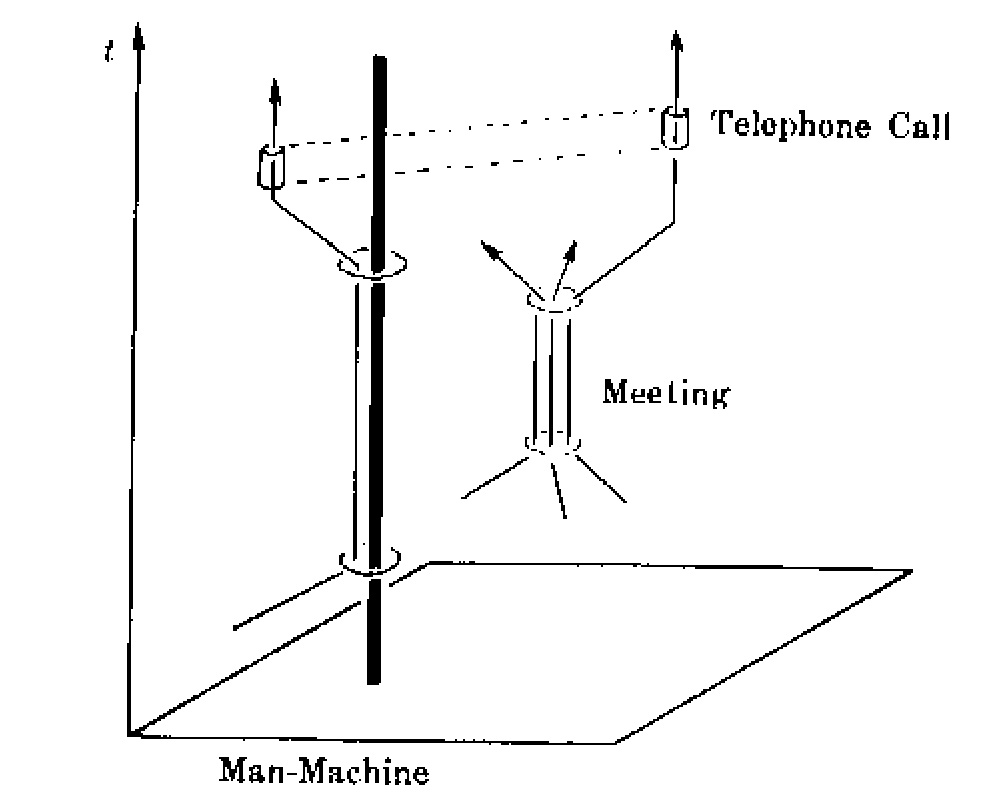
\includegraphics[width=0.9\textwidth]{figures/time-cube}
\end{center}
  \caption{Space-time prism, reproduced from \cite{Heagerstraand:1970ys}}
  \label{fig:prism}
\end{figure}

Instead of focusing on open ended possibilities, \citet{Heagerstraand:1970ys} instead chose to focus on the limits to an individual's freedom to move between places or perform activities  \citep[208]{10.2307/142726}. These were grouped into three constraints: capability constrains, which are limits to the available actions due to biology or tools, coupling constrains are limits due to the need to join with other individuals (or objects) to perform activities, authority constraints being those limits imposed by an authority. There is clearly a question as to whether cultures and societies studied archaeologically are subject to the same constraints, a premise of time-geography is that such constraints are universal and to truly benefit from it, this would have to be assumed. More challenging, perhaps, is the identification of evidence for the affects of such constraints. Time-geography focuses on hypothetical, rather than specific, individuals. It's advocates do not recommend following subjects around to create an inventory of how individuals spend their time, instead ``in choosing to develop a theoretical construct which reveals specific interactional and transactional constraints H{\"a}gerstraand is, in essence, rejecting any effort to directly predict individual behaviour'' \citep[210]{10.2307/142726}. Such a focus of analysis resonates with archaeological study, as it is not possible to trace the time-space path of specific individuals, but space and time as lived in and created by individuals is what is ultimately being studied, to put succinctly, it is the study of individuals, but not of an individual.

An area where time-geography could be particularly relevant to archaeology is simulation; in fact H{\"a}gerstraand himself suggested the use of simulation as analysis (until mathematical tools become available) \citep[21]{Heagerstraand:1970ys}. Simulation would particularly suit the idea of studying the constraints on individuals, in aggregate, or what \citet{10.2307/142726} calls the choreography of existence, it would also suit the second level of analysis, the physical existence of society, the pairing up between population and activity systems \citep[209]{10.2307/142726} and finally the prerequisite analysis required by \citet[214]{10.2307/142726} of singling out appropriate populations and applying aggregating procedures is less of a concern for a simulation as this can be included as part of the data generation step.

Returning to the focus of this chapter, the questions that can be asked of data, time-geography can be applied to understanding the constraints as identified by H{\"a}gerstraand, it can also examine how ideas, values, institutions, technology and natural rhythms interplay with the time-geographic routines of individuals and society as a whole \citep[213]{10.2307/142726}. Although it has been suggested that time-geography is not suited to the consideration of subjective constraints, psychological factors, cultural norms and social status \citep[218]{10.2307/142726} it is likely that some of these, specifically cultural norms and social status, will have some overlap with authority  and coupling constraints so need not be excluded altogether. The ideas of H{\"a}gerstraand have been developed in many different directions, of particular relevance to archaeology is the inclusion of phenomenological thinking, for example \citet{dur196} takes a two fold approach, firstly a sense of lived space-time drawing on the work of Merleau-Ponty and secondly by inclusion of the autonomous subject of Heidegger \citep[197]{dur196}. The result is a refashioned time-geography ``so that the paths retain the sense of expectation and memory suggested by Merleau-Ponty and Heidegger. A sense of space-time that brings the virtual into the experience of space, that thinks of space as connected to time'' \citep[206]{dur196} specifically focusing on the how past and future connect and are bound into the present and how ``Time is an experience of flow'' \citep[206]{dur196}. While the original concept of H{\"a}gerstraand involved a focusing on people, the inclusion of phenomenological thinking takes this one step further, to a sense of lived time-space. Another example of the combination of a social philosophy with time-geography is \citet{Pred1981-PREPEP} which overviews the concept of power with regard to social relations, attempts to conceptualise situations of power production, reproduction and transformation as part of a continual process of structuration, and portrays that process in terms of the continuous intersection of individual paths with institutional projects at specific temporal and spatial locations. The approach taken by \citet{Pred1981-PREPEP} while drawing heavily on social theory, is clearly rooted in the time-geographic tradition, placing the theory within the world of life-paths and constraints, dealing with the world as experienced by individuals, but not getting lost in the subjective experience or experience of a specific individual.

While the archaeological interest in phenomenology is extensive, the use of time-geography is much more limited and the two combined non-existent. Phenomenological thinking is not new to archaeology, however its application to time-geographic concepts presents many complications as well as opportunities when attempting to apply them to archaeological data. The study of the lived experience of time-geography surely is more than just the study of the experience of time-space as described by \citet{dur196}, a fundamental component must also be the lived experience of the constraints that are so central to time-geography. But experience is a fundamentally subjective factor and according to \citet[218]{10.2307/142726} such psychological, cultural or social constrains are excluded from the purview of time-geography. They would be challenging to study, with the focus of time-geography on exploring time-space through constraints on hypothetical individuals, but experience comes ultimately from a specific individual. Archaeologically the evidence for studying phenomenological experience is limited. \citet{fleming_2005} argues it is ``much more dependent on rhetoric, speculation, argument by assertion, and observations not always replicable when checked'' \citep[930]{fleming_2005}, and the evidence for the experience of time-space constraints is likely to be even more limited. However this does not mean that time-geography inspired studies should gloss over the fact that the constraints under study, and time-space itself are ultimately experienced by individuals.

The practical application of time-geography has focused heavily on planning contexts \citep[211]{10.2307/142726} and has been rarely applied to archaeological studies. In a recent attempt at integrating time-geographic techniques into archaeological analysis \citet{mlekuvz2010time} analysed travel times between two Roman towns using a cost surface analysis influenced by the constraints approach of time-geography. The study takes key capability constraints, such as the constraint that nobody can be in two places at the same time and that movement is time consuming as its time-geographic basis and constructs a space-time prism between the two towns, and makes an assumption of rational behaviour on the part of past agents. Ultimately the study created two models \citep[362]{mlekuvz2010time}, one of how accessible different parts of the landscape were from the location of known sites, within a given time budget and the other showing the number of points within a given time budget from which a location is accessible. The study is a very innovative method of combining the constraints of time-geography with a notion of the world as experienced in an archaeological context. Unfortunately it is purely speculative, no archaeological data is used in the process and the underlying assumption of (modern) rationality, while not entirely unreasonable without evidence to the contrary, is also unfounded. Crucially the resultant models are mostly influenced by the geographic structure of the landscape, the second model, entirely so. This assumes that the route choice is entirely driven by the environment, and is not altered by any joining or authority constraints, or any cultural factors. While mobility and movement are convenient means of attempting to understand the past as experienced, the results from the study are unfortunately highly speculative. In concluding \citep[364]{mlekuvz2010time} notes that ``time-geography does not come loaded with theoretical baggage'' which is surely a naive interpretation of a well established tradition of investigation and reasoning about people, the discussion above clearly demonstrates how different theoretical traditions have sought to adopt and influence time-geography in different directions, to adopt it uncritically is clearly a risky endeavour.

A second recent attempt at applying time-geography to archaeological data is \citet{doi:10.1559/152304009788988297} which is much more focused on the creation of software to display space-time prisms than it is on archaeological application or time-geographic concepts. Fundamentally it is a way of generating colourful (and confusing) diagrams, it does not consider time-geographic concepts, such as bundling or even constraints. The only representation of duration is on a site basis \citep[252]{doi:10.1559/152304009788988297}, as sites are static points in space (especially at a regional level) they need hardly have bothered presenting a diagram of the duration of site us in a space-time cube. The representation of duration is based on firm start and end dates, the tool is not capable of coping with one of the most common format of archaeological dates, the radiocarbon date. Fundamentally the tool does not consider people, and so is unrelated to time-geography in its entirety, it is barely capable of working with archaeological evidence and the analysis is based upon a comparison of pre-determined site attributes, which in this example are all environmental or geographic characteristics of the sites, such as slope, aspect, etc. Finally the available analytical procedures are limited and simplistic in nature. Clearly \citet{doi:10.1559/152304009788988297} have created a powerful tool, but one which was not designed with archaeological data in mind, while it has been influenced by time-geography it does not afford any analysis that is time-geographic and ultimately it does not consider people, a fundamental of time-geographic thought.

The influence of time-geography on archaeology has been more broad than the small number of studies attempting characteristically time-geographical analysis. It has also influenced interpretations more generally, such as \citet{barrett1994fragments} who considers the utilisation of time \citep[72]{barrett1994fragments} and interactions between people \citep[74]{barrett1994fragments} from a time-geographical perspective.

\section{Alternative Approach to Questions}
Having considered what are arguably the main approaches to temporal theory, it is now time to think about how this theory might be used to get the most out of spatio-temporal data. This must be more than simply taking the examples and time scales provided by others and applying them to new sites, as the questions asked must be applicable to the data available. In the same vein, there is also no need to be constrained, for example by only considering the four scales analysed by \citet{Bradley:2002fk}. Lucas clearly has this in mind when he states ``there is a lot more scope for exploring time in past societies, especially how it inflects with other social practices and concepts, such as power and gender'' \citep[118]{Lucas:2005fk}. He then suggests a potential line of inquiry ``to what extent did different sections of a prehistoric community experience time differently, and in association with what contexts?'' \citep[118]{Lucas:2005fk}. Lucas also suggests examining what he calls associated temporal concepts, such as remembering and forgetting, old and new, continuity and change \citep[94]{Lucas:2005fk}, again these are only examples, what is in many ways more significant is that there is clearly plenty of opportunity for exploring time. That such questions about society can be answered with the aid of computational methods is demonstrated by certain spatial studies, for example \citet{Kosiba:2013fk} used GIS methods to explore how social differences are embedded in spatial boundaries in the Inka empire. Using primarily visibility analysis they were able to determine restricted, exclusive ceremonial, and residential areas, \citep[93]{Kosiba:2013fk} and turned the identified spatial boundaries into social ones, thus developing an understanding of how the social perception and experience was shaped by political forces \citep[94]{Kosiba:2013fk}.

From the perspective of an individual site, there is clearly plenty of potential to examine the changes between key phases of use, for example at Hambledon it may be possible to consider how the Mesolithic use related to the Neolithic uses. During the Neolithic the site was used intermittently \citep[755]{Mercer:2008fk}, which provides a great deal of scope for spatio-temporal analysis, in particular, were the same parts of site used together, or is there evidence for a change in the locus of use over time? Does the usage appear to be the same over a long period, and can this suggest a continuity of belief? Could the site be seen as a tool for maintaining social protocols over a period of time? The excavator suggests the use may have been infrequent \citep[755]{Mercer:2008fk} in which case might each event have required a reinterpretation of the site, of the physical remains that were found and re-worked at each event? Each period of use would surely have been influenced by those remains from the past that were extant at the time. Along a similar vein, episodes of re-digging of ditches would likely result in deposited material from the past being excavated, although clearly the finding of articulated remains demonstrates that some areas were not re-dug, possibly by chance, or maybe due to the memory of their location, potentially aided by physical reminders, \citep[759]{Mercer:2008fk}. In fact, the excavator does suggest that the uses of particular ditch segments were remembered with the same type of use occurring over a long period of time \citep[756]{Mercer:2008fk}. 

There is also the potential to consider multiple timescales, from the short-term events, to the longer scale of monument construction and Hambledon's place in social networks. Clearly there are opportunities for exploring long term processes, such as repeated re-use of particular areas, also the suggestion from the excavator that the more defensive elements were potentially built to follow a plan of some sort \citep[760]{Mercer:2008fk}. It also might only be over longer time frames that the changes to areas that are a focus for use become apparent, with such drift, or relocation of activity hidden by noise at a smaller scale. Finally it may be possible to consider how use in the later phases was influenced by the remains of much earlier activity, in particular the excavators assertion that the enclosure was recognised, and used, into the second millennium BC \citep[770]{Mercer:2008fk}. However, at some point subsequent to that, it was disregarded, and by the Iron Age, there was a field system laid out as though earlier earthworks no longer existed \citep[770]{Mercer:2008fk}.

From a larger spatial perspective the Gathering Time project \citep{Whittle:2011kl,Whittle:2011tg} offers the ability to consider similar site-level questions, but across multiple sites and a comparison of the answers. At the inter-site level, similar questions could be asked of landscapes, such as how existing monuments affect the building of new monuments, both of the same type and of entirely different types. In addition monuments need not be considered a totality, depending on the resolution of the temporal data it may be possible to analyse the spatial dimension of the alteration of sites, for example do particular alterations happen within a constrained timeframe across sites in a particular locality.

Finally, at a national, or inter-national level there is the potential to not only examine larger processes, but also tie these back down to local phenomena, for example Bradley's potential link between long house orientation, and the notion of ancestral homelands. There is an enormous amount of scope at this layer for a wide variety of potential lines of inquiry, other examples could include, taking current spatio-temporal approaches on the spread of the Neolithic, and examining notions of past and identity, how did incoming people or ideas affect a populations view of its own past, its traditions and heritage. \citet{BocquetAppel2009807} identified that the process was not smooth, so during the periods of pause, and then subsequent rapid spread, how did that affect notions of the past? Presumably if pauses lasted for generations the new ideas or new people would become incumbent, a part of the status quo and the inherited past in these areas would be different (at least at first) from that of areas of rapid change. A recent example of such a study is \citet{whittle2018times} which considers a range of themes and sites across Europe and at different scales of time.

This chapter has considered both routine and more theory driven approaches to the questions that have been asked of archaeological remains. Specifically, but not exclusively, temporal questions, how such questions can trivially be extended into the spatial domain and some hypothetical lines of enquiry. Next, we will consider the kind of methods that can analyse the archaeological remains, or raw data. The analysis will be used to take a step towards answering questions that go beyond the descriptive. %9,430 #13,520
\chapter{Methods for Data Analysis} %8000
\label{ch:analysis}
Having looked at the kinds of questions that should be being asked, we will now turn to examine the methods that might be used to help answer those questions, and more importantly  to criticisms of those methods. In order to get the most out of these methods it is important that they are used within the limits of their applicability, the best way to assess this is by critical assessment of their use. There have been comparatively few quantitative spatio-temporal methods developed, when compared to purely temporal or spatial techniques. Of these, the vast majority are spatial methods.

\section{Spatial Analysis}
There are a variety of different ways of slicing up the large number of techniques for analysing spatial data, they will not all be catalogued here. The different theoretical schools of thought such methods are influenced by will only be roughly categorised. Modern approaches to Landscape analysis are often split into experiential/phenomenological or GIS based quantitative analysis \citep[491]{GravesMcEwan2012}. While there have been attempts to draw both schools of thought together, (e.g. \citealp{Lake:2007fk}) and even creating combined methods, such as \citet{Rennell2012}, \citet{Eve2012} and \citet{Millican2012}, this has not been hugely successful. 

With regard to criticisms of GIS based techniques, these are often either from a theoretical perspective, or a methodological perspective. With regard to the first category of criticisms, Llobera, an influential GIS practitioner, readily admits that when GIS is measured against Phenomenology's theoretical aims it falls short \citep[497]{Llobera2012}. Clearly this is not surprising and in fact ``this inferiority is rather a matter of opinion especially when compared against methods (if any) put forward within mainstream narratives'' \citep[498]{Llobera2012}. The theoretical elements of these criticisms are well rehearsed, focussing around dogmatic rejection of representations, particularly digital ones and have been addressed by \citet[498]{Llobera2012}. In fact Llobera concludes that the main criticisms in this vein are ``for the most part too generic or inconsistent to be constructive'' \citep[499]{Llobera2012}. \citet{eps364158} focuses on two key criticisms raised against visibility studies, firstly the objection that map like representations are specifically a modern, western construction, which we cannot assume is shared by other cultures \citep[118]{eps364158}. And secondly the suggestion that such studies privilege vision over other aspects of bodily engagement \citep[118]{eps364158}. With regard to the first, after considering early evidence of map creation and map like thinking from cultures as diverse (spatially and temporally) as ancient Peru and Babylonia Wheatley robustly disregards the criticism: ``There are good reasons, then, not to uncritically accept the assertion that non-western, non-modern cultures cannot or could not engage in this kind of spatial abstraction'' \citep[119]{eps364158}. However he does note, that this line of critique can be constructive, in forcing us to consider the culturally specific ways we currently use to represent space \citep[118]{eps364158}. With the second criticism, however,  Wheatley has some sympathy, he concludes that while there is evidence that vision may be naturally privileged by humans, we are not solely visual creatures \citep[121]{eps364158} and that ``a more interesting line of investigation would therefore lead to the development of methods for exploring how the senses may be related to one another in the structuring of space'' \citep[121]{eps364158}.

From some of the more nuanced criticism it is possible to discern methodological issues that must be considered when such analytical methods are employed, for example \citet{Llobera2012} identifies:
\begin{enumerate}
\item inadequacies with spatial methods to address the kind of questions asked by interpretive approaches
\item spatial representations are often abstracted, mismatched in terms of scale and precision from the questions asked
\item GIS often does not deal with space as it surrounds an individual
\end{enumerate}

To this can be added the recommendation from \citet{eps364158}, that there is clear potential in considering how the senses operate together to create an experience of place. Going further, there is clearly the opportunity to explore how this could translate into spatial patterning \citep[122]{eps364158}, modulated by spatial scale \citep[123]{eps364158}, which would ``offer the possibility of methodological application because they can be modelled and so are amenable to the development of robust, formal methods while they remain at the same time deeply relational and contextual'' \citep[124]{eps364158}.

Other specific, methodological issues, often raised by GIS practitioners themselves, are crucial when considering the specific analytical method, but have less impact on the wider issue of GIS based quantitative analysis. However, there have been wider criticisms raised, for example the notion of the theoretical neutrality of GIS has been considered indefensible since \citet{Wheatley:1993qf}. With this in mind, it is important that analytical techniques are not simply applied as mere tools, but that their theoretical underpinnings are understood. 

Apart from the correct application of appropriate methods, a key area of improvement would be the alignment of appropriate methods with questions. A complaint raised against many methods is that they are epistemologically limited and encourage the creation of an objectified, god's eye view \citep[512]{Rennell2012}, which is the source of the mismatch between our knowledge about the world, and our knowledge about the world as experienced \citep[498]{Llobera2012}, although \citet{eps364158} argues contrary to this, as discussed above. A part of this problem is that most spatial analysis often lacks any consideration of the temporal structure of space, as such geographical areas are represented in an idealised a-temporal way. For example, \citet{wheatley1995cumulative} presents all the sites as though outside of time, as there is no consideration of the sequencing of the construction of monuments, and therefore of the incremental changes to the visual structure of the landscape. By combining time and space into the same analysis it will be much easier to represent the world as it may be have been. And it may in fact add an extra dimension of being-in-the-world, by studying sites at particular points in time and in their history. 

Before delving into time, let us track back slightly, and consider the other main spatial approach, the experiential or phenomenological landscape approach. This is not without its critiques, although \citet[512]{Rennell2012} argues that many criticisms are still raised against older, more provocative pieces of phenomenological writings and lump these with progressive subject centred approaches, without considering their distinctions. A particularly important criticism is the lack of dialogue, especially from the experiential side of the argument \citep[601]{Gillings2012}, without which it is difficult to forge a unified approach to landscape analysis. In fact, Gillings goes on to suggest that the two approaches are intractable and that it would be more profitable for quantitative researchers to develop their own theoretical frameworks \citep[610]{Gillings2012}. Others have suggested techniques, such as scaffolding methods, should be used to bridge the gap between empirical information and narratives \citep{Llobera2012}. This difficulty in going from theory to method has been recognised (e.g. \citealp[500]{Llobera2012}) as more complicated for certain theories, such as phenomenological derived ones, with part of the problem being the lack of a defined body of theory, and the focus of such theories on ``complexity through detailed context-rich narratives'' \citep[503]{Llobera2012}. This clearly relates to the previous chapters examination of the questions that are asked, however as this project is approaching combined spatio-temporal analysis from the angle of spatialising time, a thorough analysis and appraisal of spatial questions and how phenomenological questions can be answered by GIS will be left for the future, perhaps, for a project to temporalise space.

In terms of phenomenological or subject-centred approaches to analysis, a critical concern from a temporal perspective, is that such analysis are based firmly in the present and pay little regard to the changes that will have taken place in the landscape over time. As such, it is really only possible to study modern people's relationships with a site, or landscape and infer back to the experiences of past people. But surely, to truly understand the experiences of people in the past it is essential to attempt to understand the landscape as it was, for people then and through the ages, how it has developed through time, including peoples relationship with their past through the landscape. Is it truly feasible, for a modern archaeologist to understand a past person's relationship with their past by simple experiencing a modern landscape? 

\section{Temporal Analysis}
There are few quantitative temporal analytical techniques, fewer still that are routinely applied to archaeological questions, with most studies taking a more narrative or descriptive approach (e.g. \citealp{Bradley:2002fk,Bailey:2007fk}). This is perhaps because it is hard to completely remove the spatial component. There has been some interest in aoristic based approaches, such as \citet{Crema2012} and \citet{Baxter2016120}, although most aoristic analysis has been spatio-temporal, so will be covered in section~\ref{sec:sta} below. The two most prominent forms of temporal analysis are bayesian modelling and summed probability distribution, both approaches operate (primarily) with radiocarbon dates, the merits and criticisms of both shall be considered in turn.

\subsection{Bayesian Modelling}
Probably the most frequently used quantitative temporal approach is the bayesian modelling of radiocarbon dates, which has increased in use dramatically from around 2006 onwards, \citep[679]{doi:10.1080/00438243.2015.1067640} and which forms a core part of large scale projects such as Gathering Time \citep{Whittle:2011kl,Whittle:2011tg} and the Times of Their Lives \citep{whittle2018times}. The claims for this approach are considerable, including being a third radiocarbon revolution \citep[126]{azu_rc3483}, and that it can in some cases produce chronologies with a resolution of decades \citep[141]{azu_rc3483} although, it should be noted that the approach is not limited to radiocarbon determinations \citep{Millard:2003fk}. However, as an approach it is not without issues, with several recent works taking a critical evaluation to the corpus of studies using bayesian methods to model dates\citep[e.g.][]{doi:10.1080/00438243.2015.1070082,doi:10.1080/00438243.2015.1053977,doi:10.1080/00438243.2015.1065759}. Some of the common themes of such criticisms include:

\subsubsection{Validity of the Model}
The validity of the model is one of the two main issues identified by \citet{doi:10.1080/00438243.2015.1070082}. Fundamentally it is about whether the archaeologist's interpretation of the chronology as represented in the model is valid. There are more detailed nuances, such as: whether the questions the archaeologist is trying to answer are amenable to modelling; if they will be answered by this model \citep[531]{doi:10.1080/00438243.2015.1070082}; and the archaeologist's skill in constructing models, for example whether the use of boundaries is valid \citep[533]{doi:10.1080/00438243.2015.1070082}. A robust example of this is presented in \citet{doi:10.1080/00438243.2015.1065759} when examining bayesian modelling of Palaeolithic dates. The issue is encountered in the first instance by assuming a Mousterian overlap with the Ch\^atelperronian, as evidenced by dating Mousterian sites outside of the Ch\^atelperronian's known distribution, and secondly by combining evidence for human and carnivore occupations in the same phase in the model \citep[603]{doi:10.1080/00438243.2015.1065759}. This issue can be thought of as ``the relationship between the dated event and the target event'' \citep[689]{doi:10.1080/00438243.2015.1067640} and it is important that the modeller is sure of the association between the two events, in particular they must be confident they can determine if a sample is residual or intrusive. While it may be impossible to guard against this issue entirely, as it is in part down to subjective interpretation, it is crucial that the modeller understands the implications of choices made when constructing the model. Further protection can in this case be provided by critical review and re-evaluation of published models \cite{doi:10.1080/00438243.2015.1070082}.

\subsubsection{Reliability of Prior Information}
Reliability of prior information is the second of the two main issues covered by \citet{doi:10.1080/00438243.2015.1070082}; it ultimately boils down to the reliability and applicability of the dated samples. In fact, they assert that ``the main responsibility of archaeological users of bayesian models is to ensure the reliability of the prior information upon which models are based'' \citep[527]{doi:10.1080/00438243.2015.1070082}. Clearly there is some overlap with the previous criticism, in particular with assessing residuality. There are some clear guidelines, which can be used to increase confidence in chosen priors, for example ``dated samples must reflect human activity'' \citep[532]{doi:10.1080/00438243.2015.1070082} and it is important to be confident in their stratigraphic location. It is also recommended that all priors be justified by the modeller \citep[537]{doi:10.1080/00438243.2015.1070082}. \citet{doi:10.1080/00438243.2015.1067640} recommends authors provide sufficient details of their priors, such that their reliability can be easily assessed by others. This would include: calculation details, references to laboratory methods, associated measurements \citep[687]{doi:10.1080/00438243.2015.1067640}, and ideally also other details such as carbon reservoir, age at death, single entity, etc \citep[690]{doi:10.1080/00438243.2015.1067640}. These are not mere technical details, for example, \citet[610]{doi:10.1080/00438243.2015.1065759} discuss the effect of dragging of modelled dates by the inclusion of older dates, which don't use modern pre-treatment methods. And it is perhaps for this reason that \citet{doi:10.1080/00438243.2015.1070082} recommend that samples should only be included in a model if they have been subject to robust pre-treatment methods, which are fully delineated \citep[537]{doi:10.1080/00438243.2015.1070082}.

\subsubsection{Small Numbers of Priors}
A small number of priors is a problem encountered by \citet[604]{doi:10.1080/00438243.2015.1065759}, where the limited number of dates in a model means it is highly sensitive to each individual prior. On a similar vein \citet{doi:10.1080/00438243.2015.1070082} pose the question ``another source of error is when single layers are represented by only one radiocarbon measurement. How do we know if this is accurate?'' \citep[530]{doi:10.1080/00438243.2015.1070082}. Related to this problem is that of selecting samples, as \citet{doi:10.1080/00438243.2015.1070082} notes, when samples are reviewed critically the pool of suitable samples diminishes. However this does not mean samples should be used un-critically, instead we must be wary of models which rely heavily on a small number of samples and where possible try to obtain more high quality samples.

\subsubsection{Uncritical Acceptance of Posterior Results}
The problem of uncritical acceptance of posterior results has been identified by \citet[528]{doi:10.1080/00438243.2015.1070082} and relates to the uncritical acceptance of posterior results from priors or models with one or more of the previous issues. This data is then fed into further analysis where it is accepted at face value. Surely, any inferences drawn from such a bayesian model should have the same, if not greater uncertainty than their constituent parts. In fact if we are suspicious of a prior value, why include it in a model in the first place? The result of this is a situation where the probability distribution is not necessarily representative of the actual probability; if there are samples with some doubt attached surely this should be modelled, so that the doubt is represented in the probability distribution, or dubious results should simply be discounted.

\subsubsection{Bayesian Analysis in Gathering Time}
The bayesian analysis of Gathering Time seeks to create an almost historical narrative of the early Neolithic \citep[800]{Whittle:2011tg}, with a particular focus on the enclosures of southern Britain. This is achieved by building up an increasingly abstracted view of dates from such enclosures. The process starts at the smallest level, each dated sample is listed and described, e.g. for Windmill Hill see \citet[68]{Whittle:2011kl}. These dates are then combined into a bayesian model of the chronology (e.g., \citealp[83]{Whittle:2011kl}) which for larger sites is done in sections with another more abstracted model created for the whole site e.g. \citealp[83]{Whittle:2011kl}. A key part of these models is the generation of so called boundary events: at the very least there will be a start and end for each site, depending on the extent of dating and specific research questions, often more. The boundary events for all the sites in a wider geographical area, such as the North Wiltshire Downs are used to build a model for that wider area, (e.g. \citealp[106]{Whittle:2011kl}) even larger areas, such as southern, or eastern England are then considered in the same way (e.g. \citealp[684]{Whittle:2011tg}). Finally, further models are derived, for the start of all southern British enclosures (e.g., \citealp[687]{Whittle:2011tg}) and derived data, such as the duration of use across all enclosures (e.g. \citealp[706]{Whittle:2011tg}). The authors also construct models for other types of data, such as long barrows, linear monuments, and pottery. The refined dates provided by the large number of bayesian models are then used to build up a narrative of the early British Neolithic \citep[800]{Whittle:2011tg}. Tying all the different elements together into a unified proto-history of where practices and material culture first appeared and the rate at which it spread over the country.

The process taken to build up these models (unsurprisingly) meets the criteria as set out by \citet{doi:10.1080/00438243.2015.1067640} covering the themes identified above as validity of the model and reliability of prior information. However, the themes of small numbers of priors and of uncritical acceptance of posterior results require further investigation. Of the 38 enclosures examined in the text (more are included, but have no dates), there is quite a range in the number of dates per site. The smallest number of dates for a site that are included in the models is one, Combe Hill, while the largest is Hambledon Hill with 162. In this case, Combe Hill is modelled differently to Hambledon (as a TAQ in \citealp[687]{Whittle:2011tg}). The site with the smallest number of dates that is included in the model as a first class entity (in the same way Hambledon is included, by boundary values) is Court Hill, which has two dates in its model. Figure~\ref{fig:date-counts} shows a histogram of the number of dates or samples used in the study, the line widths being five dates. It clearly shows that the vast majority (23) sites have fewer than ten dates, ten sites have between 20 and 33 dates, and one each has 43, 46, 62, 76 and 162 dates. 

\begin{figure}
\centering
	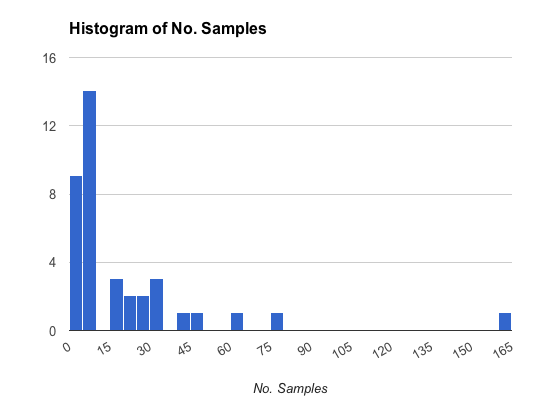
\includegraphics[width=0.6\textwidth]{figures/date-counts}
  \caption{Histogram of number of dated samples for sites included in Gathering Time}
  \label{fig:date-counts}
\end{figure}

Once these sites are abstracted away from their original models into boundary events they are (apart from Combe Hill) all represented in the same way, there is no indicator of the strength of evidence that lies behind these values. Such a metric could be taken as a measure of durability of the value, for example it is less likely the start and end dates calculated for Hambledon Hill will be refined by further fieldwork, but it is quite likely, even probable that more fieldwork would result in the values for Court Hill to be updated.

The abstraction of models into boundary events causes other problems. A clear example is Whitehawk Camp, where the limitations of the dating evidence are made clear in the text, for example the ``only dateable material from the primary chalk rubble in Ditch II is a residue sample from a single sherd, which could have been redeposited. The date of Ditch IV depends on non-optimal samples, and those for both Ditches III and IV may relate to cuts rather than to the original circuits.'' \citep[226]{Whittle:2011kl}. However this does not stop the abstracted boundary events to be included in other models, at which point they are taken to be as valid as any other value. As well as the formal uncertainty of the radiocarbon dates, there is also an informal uncertainty of the validity of the dates (and in other cases the model e.g. at Haddenham, \citealp[277]{Whittle:2011kl}) but which disappears once sites have been abstracted to boundary events. While the alteration of a few dates is unlikely to make a big difference to the macro scale result, it might have been worth the authors exploring how much influence they had on the result, by running it again without boundary dates from sites with dubious dating evidence. More problematic would be an issue with a large number of sites.

The large number of sites with very few dates also points at a further potential problem, that of the limited spatial extent of archaeological investigations. For example at Court Hill, the area excavated was around 5m of ditch, out of around 175m \citep[242]{Whittle:2011kl} that is roughly 2.9\%. How confident are they that the reported dates accurately represent the start of activity at Court Hill? It is quite possible the site was dug over a period of time, as a succession of ditch segments, until it was completed and then underwent subsequent further use. Clearly, this is a problem with sites that have only undergone small archaeological investigations, with ultimately the only solution being to commission a full research programme on these sites. But this problem is not only limited to sites with a handful of dates, for example at Windmill Hill the inner ditch dates come from only four sections of ditch, the outer ditch dates come from only five sections, with less than 10\% of it having been excavated \citep[63]{Whittle:2011kl}. It is from this paucity of dated ditches that the inner-outer-middle order of construction is derived (which is in fact only 59\% probable \citealp[91]{Whittle:2011kl}) and it does not take into account the duration of the construction, only of use. In this model, each circuit is fully constructed before the next one is begun \citep[91]{Whittle:2011kl}. To a greater or lesser extent, this is a problem with all the enclosures examined in Gathering Time, caused in part by varying degrees of excavation, and also by the difficulty in finding suitable samples to date, especially in archived material. While total excavation might be ideal from the point of view of obtaining all possible data, it leaves nothing for future generations and is also extremely unlikely due to the cost and time it would take. A much more feasible approach is to make sure that excavated areas are relatively evenly distributed around the enclosure, as at Northborough \citep[328]{Whittle:2011kl} or Bury Hill \citep[240]{Whittle:2011kl} rather than The Trundle where all excavation is concentrated in one small area \citep[233]{Whittle:2011kl}. A not insignificant issue in Gathering Time is the difficulty of working out what the extent of excavated area is and from where around the enclosure circuit the dates have come from. For a start not every site has a plan, e.g. Maiden Bower \citep[265]{Whittle:2011kl} and those that do are of varying format and quality.

The lack of spatiality also extends to the larger scale analysis, for example, the analysis of Hambledon Hill within Cranborne Chase \citep[151]{Whittle:2011kl} lacks any plan and each regional analysis has only one large scale plan. The regional discussions do not provide maps that are more detailed or plans to illustrate the discussion and in fact hardly consider the spatial relationships and characteristics of the sites. There is also no attempt to match the humanising of time (through lifespans) with a humanising of space (by distance in travel times).

In summary, when done well the results from applying bayesian modelling to dates can be powerful, but unfortunately, it is not always done well. In an effort to improve quality, several authors have published best practices, for example \citet{doi:10.1080/00438243.2015.1067640}. However, it is clearly important that bayesian results are critically evaluated, and not simply accepted at face value. 

\subsection{Summed Radiocarbon Distributions}
Summed radiocarbon dates have been used as a method for determining the duration of archaeological phases \citep[9]{CAJ:676108} however when compared to bayesian methods they were found to create erroneously long estimates for durations of activity \citep[10]{CAJ:676108}. The problem is due to an implicit assumption that all the uncertainties are independent \citep[11]{CAJ:676108}. However the method is still used, a recent example of such an approach is demonstrated in \citet{AQY:9508563}, which compares summed radiocarbon probabilities across cultures, and bases its analysis on the assumption of random sampling \citep[1079]{AQY:9508563} contra \citet{CAJ:676108}. 

Summed radiocarbon dates have also been used contentiously as a proxy for population, with bold claims being made on the back of such analysis. A recent example of which is \citet{Shennan:2013fk} claiming patterns of population boom and bust in Neolithic Europe, and \citet{Collard2010866} using the method to show ``the Neolithic transition in Britain was mediated by a large influx of farmers from continental Europe''  \citep[869]{Collard2010866}. There has been a considerable amount of work undertaken to perfect the technique, for example correcting for statistical artefacts introduced by the calibration process, or for taphonomic loss such as by \citet{Williams2012578}. The methods used in such studies have become increasingly complex, for example \citet{Shennan:2013fk} take a null hypothesis approach, comparing their data set to the results from data generated by a model that exponentially increases the summed probability distribution through time. They then used a range of statistical significance tests to reject this null hypothesis and prove their conjecture - that there is a relationship between summed radiocarbon distributions and population density. 

There have been fundamental criticisms and corresponding defences of this approach, especially \citet{Torfing2015193,Timpson2015199,Torfing2015203}. Ultimately, according to \citet{Torfing2015203} the problems fall into two main areas, firstly he enumerates a set of assumptions that are required for the original assumptions of \citet{10.2307/281060} (on which the method is based) to be valid, these are:
\begin{enumerate}
\item People leave a comparable amount of material
\item All material is deposited in a similar manner that allow for equal preservation
\item Sites from all periods are equally excavated and dated
\end{enumerate}

Secondly, he analyses the use of sampling, as radiocarbon dates are often treated as a random sample. Torfing demonstrates that the ``radiocarbon date is only the last sample of a series of samples'' \citep[205]{Torfing2015203}. He goes on to argue that the link between population and radiocarbon dates is yet to be demonstrated, the lack of which could be particularly problematic if periods with different processes of site formation and preservation are compared. This criticism is effectively along the same vein as that made by \citet{CAJ:676108} about the nature of radiocarbon dates as samples. Three specific issues are analysed in \citet{Torfing2015193} as a criticism of \citet{Shennan:2013fk} and he concludes that the proposed model linking summed radiocarbon distributions and population is fundamentally flawed, ``several problems are still present: changes in monumentality, subsistence strategy and modern research foci are all systematic sources of error'' \citep[197]{Torfing2015193}.

These issues are summed up by a single succinct question, ``how does our proposed data-set relate to the questions we wish to answer?'' \citep[204]{Torfing2015203} and whereas he approaches the issues with a contextual analysis of the data, he is critical of proponents of summed probability distribution, as they ``mostly try to overcome these issues at the final step, that of the 14C-dates, and do not consider the formation of the record in the first place. The relevant problems lie outside the immediate calculations of the statistics, and are of a more fundamental character of how to use dates as data'' \citep[204]{Torfing2015203}. Specifically he is critical of the ``notion that if a large enough sample is used, and it is carefully treated with statistical tests, these sources of error will be insignificant'' \citep[193]{Torfing2015193} and argues that the quantities of datable material left by different activities are not necessarily comparable. Finally, he notes that any differences will persist in the archaeological record regardless of sample size \citep[193]{Torfing2015193}. 

In response to this criticisms \citet{Timpson2015199} respond with a mix of argument and hyperbole, including ``his subjective criticisms, lacking in any formal hypothesis testing, only serve to stagnate the discipline'' \citep[200]{Timpson2015199} and by claiming his lack of understanding of the method. They claim to be using proxies to only be showing correlation, however as \citet{Torfing2015203} points out this would only be valid if a relationship had already been proved between summed radiocarbon probabilities and population \citep[204]{Torfing2015203}. They also accuse him of not performing significance tests on his models, which is necessary due to the increase in sampling error caused by his use of specific (non random) subsets of the data \citep{Timpson2015199}. It would seem quite ironic that the proponents of a method that has been criticised for being reliant on assumptions of sample independence object to non-random sampling.

Summed radiocarbon distributions have also been used to analyse the changing importance of cereal cultivation through time by \citet{Stevens:2012fk, doi:10.1080/00438243.2015.1087330}. As with other approaches to summed radiocarbon distributions this method has not been without criticisms, \citet{doi:10.1080/00438243.2015.1072477,doi:10.1080/00438243.2015.1093427} concluded that the sample size was too small, that the results were in fact likely more to do with sampling strategy and that archaeobotanical evidence was capable of providing a much higher resolution picture of the use of cereal crops \citep[848]{doi:10.1080/00438243.2015.1072477}. 

Finally, there is a clear lack of a concern for the spatial in such studies. Taking a sample of five relatively recent studies, which are well regarded among proponents of the method, clearly demonstrates this lack. Across \citet{Shennan2013,TIMPSON2014549,10.1371/journal.pone.0105730,Shennan:2013fk,HINZ20123331} there is an average of less than one map or plan per publication and a variety of approaches for considering spatiality. \citet{Shennan2013} considers results only at the continental scale and a single region therein, where as \citet{HINZ20123331} considers 12 regions, examined in groups by the shape of results and then by comparisons across regions. Other publications sit somewhere along the spectrum from effectively a-spatial discussion to splitting an area up into a set of regions, which are examined independently. None perform any spatial analysis, or attempt to examine how population may be just as much a function of space as time, instead they simply accept the spatial variation and examine different regions separately.

The range of uses to which summed radiocarbon dates have been put suggest a fascination with them, but it is as though researchers see the distribution and think frequency, rather than probability. However, the same kinds of questions have been approached using alternative techniques, such as \citet{Steele20102017,BocquetAppel2009807}, which use a range of techniques for performing analysis on radiocarbon dates. It is to these other methods we should be turning and attempting to find ways to refine our highest quality data (such as through bayesian modelling) rather than dredging though large data sets hoping to find unproven correlations. While the summing of radiocarbon dates is primarily a temporal approach, the questions that are being asked, about the spread of Neolithic culture are fundamentally spatio-temporal in nature. Surely such questions are best answered by combined techniques, such as those that follow.

\section{Spatio-temporal Analysis} \label{sec:sta}
The number of attempted spatio-temporal analytical methods is relatively small, with some coming from research into Temporal-GIS, (hereafter T-GIS) and others as stand-alone pieces of research. The discussion of such software more generally will be deferred until the next chapter, the focus here will be on the spatio-temporal analysis performed using such systems.

One of the earliest attempts at spatio-temporal analysis (which has already been covered) was an extension of a spatial method, using the absolute date value as a property, for understanding the classic lowland Maya collapse. But it is necessary to turn to a different source to understand more recent spatio-temporal work. Johnson has had an impact as the source of multiple spatio-temporal methods, both from research into T-GIS and spatio-temporal analysis independent of such software. He was the first to build a T-GIS designed for archaeology, \citep{Johnson:1999cr, Johnson:2002kx} and also introduced aoristic analysis into archaeology \citep{Johnson:2004fk}, which has influenced a whole research tradition, e.g. \citet{Crema20101118}. 
While Johnson may have been one of the pioneers of T-GIS within archaeology, his resultant project, TimeMap does not seem to have been used for any archaeological study. Instead it has been limited to projects in the historical era, as its temporal model is unable to cope with probabilistic dates. So, in terms of spatio-temporal analytical methods TimeMap must be discounted, as it does not actually perform any that are of archaeological interest. Following on from Johnson, several authors have attempted T-GIS type systems with varying degrees of success, but few have attempted much in the way of spatio-temporal analysis. Most have simply described potential systems (e.g. \citealp{lock2002analysing}), or implemented mechanisms for storage and representation of the data. The exception to this being \citet{Green:2008fk} who implemented a T-GIS, which was then used as a platform for further analysis.

Green's analysis is mostly based around visual inspection (e.g. \citealp[156]{Green:2008fk}) of plots of radiocarbon dates. The dates are grouped by thematic layers, such as by period, these periods are then analysed sequentially, so that the result is a series of analysis of different time-slices. Crucially however, the background layer is not changed for each new time-slice and so is, in effect, static over time, for an example of this see figure~\ref{fig:green1}. The point plots for radiocarbon dates change, but the background is a map of all archaeological features from the site. This is quite problematic, as there is a logical disconnection between the dates and the archaeological features. It would make visual analysis and interpretation much easier, and more potent, if the features were associated with dates, then the combined two could be hidden or displayed for each plot. Another key problem with this is the arbitrary nature of the time slices, based on interpretative periods, as compared to other studies, which take the approach of taking time slices at regular intervals. There are problems with both approaches, for example, \citet{Crema20101118} notes that an approach with regular intervals can highlight changes within arbitrary periods. Conversely, if there is low temporal resolution between regular intervals it can appear as though there is little to no change between these intervals, but this is in fact an artefact of the data \citep[1121]{Crema20101118}. Clearly, neither approach is obviously a much better choice, this being the case we might reasonably expect an appraisal of the shortfalls of the chosen approach, but Green has not done this. 

\begin{figure}
\centering
	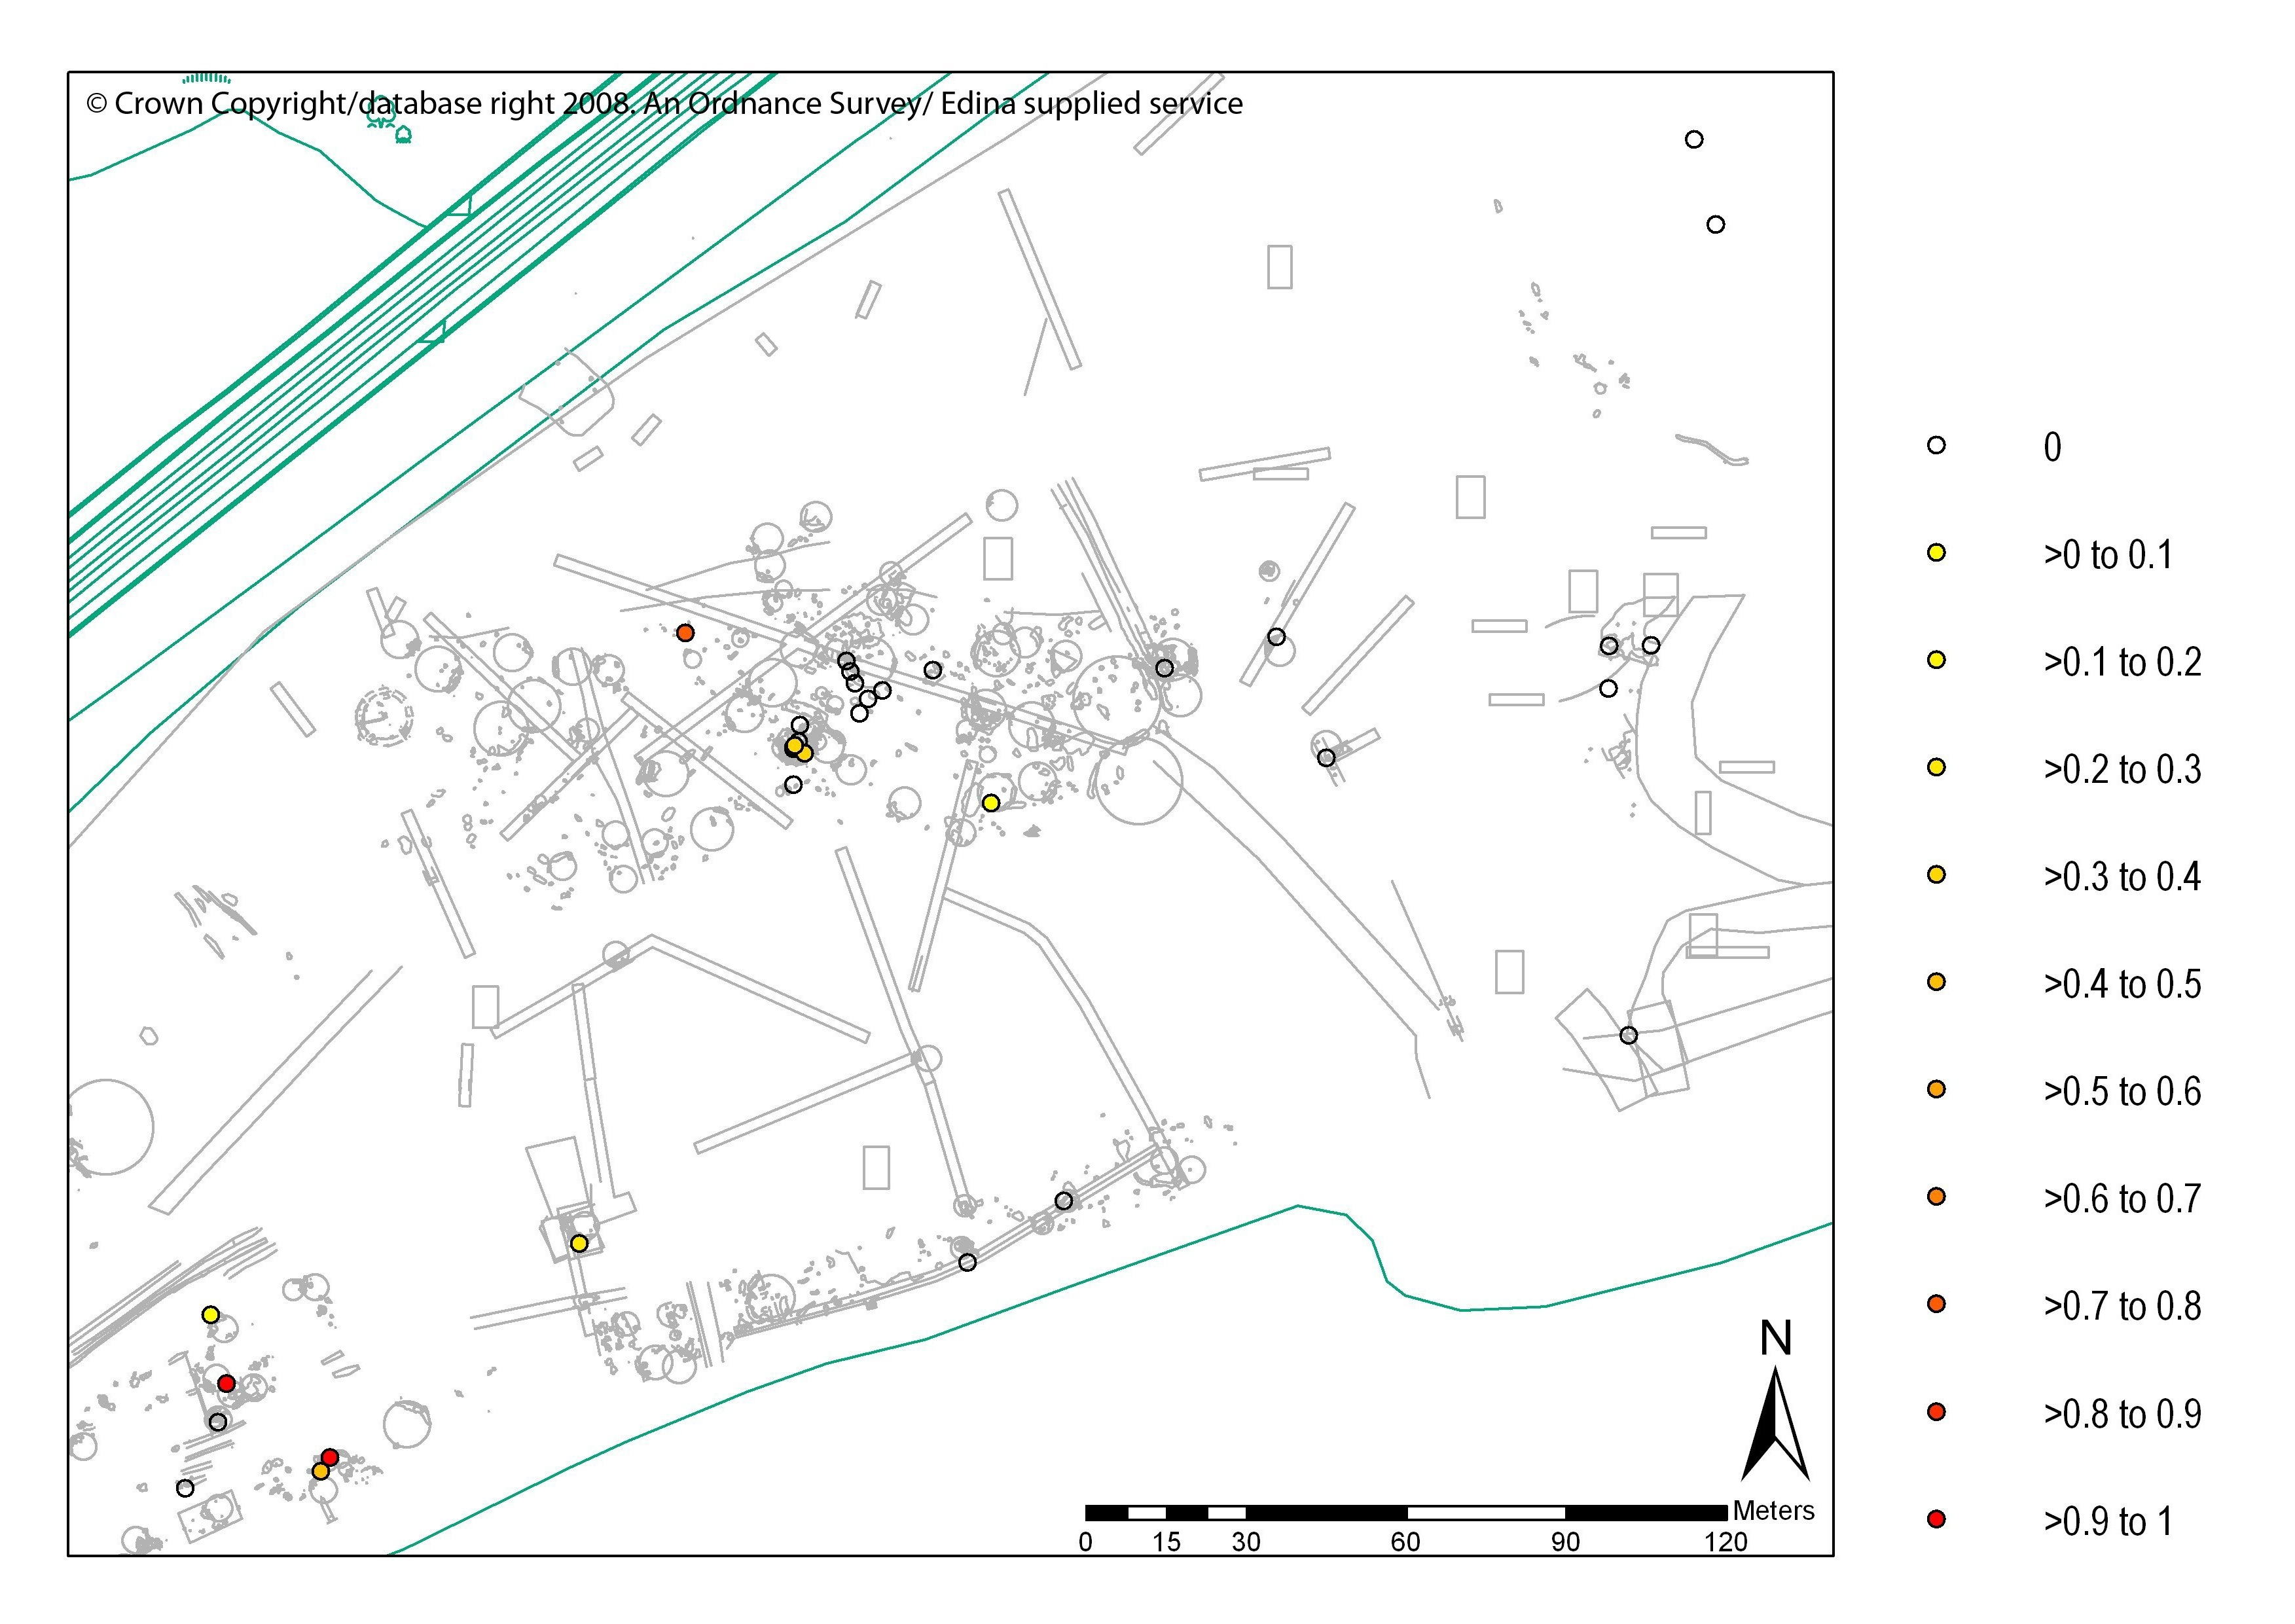
\includegraphics[width=0.9\textwidth,height=0.9\textheight,keepaspectratio=true]{figures/green1}
  \caption{Spatial distribution of un-modelled radiocarbon dates, coloured according to
probability of them falling within the period 4000-3500 cal BC, from \cite{Green:2008fk}}
  \label{fig:green1}
\end{figure}

In addition to this, Green also demonstrates the potential for spatio-temporal interpolation using his T-GIS, despite earlier in his thesis stating ``interpolation from time slices may be justified for evolutionary geographical change, but cannot capture the more random nature of cultural or historical change'' \citep[96]{Green:2008fk}, and that ``temporal interpolation of archaeology is complex and very uncertain. It is perhaps an act best left to the imagination, as computerised interpolation can give false authority to very speculative models'' \citep[98]{Green:2008fk}, and finally ``I do not believe that interpolation is the right way to approach temporal gaps in archaeological data: presenting a false completeness regarding our knowledge of the past has too great a potential to mislead.'' \citep[101]{Green:2008fk}. For two case studies Green makes use of interpolation, at an intra-site level these results ``give an indication of the probability of dates falling within any area of the site'' \citep[189]{Green:2008fk}. The analysis is performed on a per-period basis, demonstrating which areas have higher, and which have lower probabilities for a specified period. This is effectively being used as a proxy for use or activity of the site during each particular period. Of course, there are other potential reasons for lack of dates from certain areas, it may be a lack of use, it may also be down to a lack of datable material, or changing conditions. With only 65 radiocarbon determinations \citep[129]{Green:2008fk} spread across eight periods \citep[189]{Green:2008fk} they are likely to be highly influenced by any factors effecting recovery or applicability of radiocarbon methods. The validity of the interpolation then hinges on the validity of the quantity of radiocarbon dates for determining the relative past use, and of this Green does not provide evidence, especially for such a small sample size. Finally, by applying the interpolation without respect to the underlying archaeological features, the approximation of use created by the interpolation might actually be less accurate than a thorough examination of the archaeology. Specifically, it will smooth through dramatic changes in values, for example between successive indoor and outdoor spaces. See figure~\ref{fig:green2} for an example interpolation from Green's first case study, showing the interpolation overlaying features from all periods.

\begin{figure}
\centering
	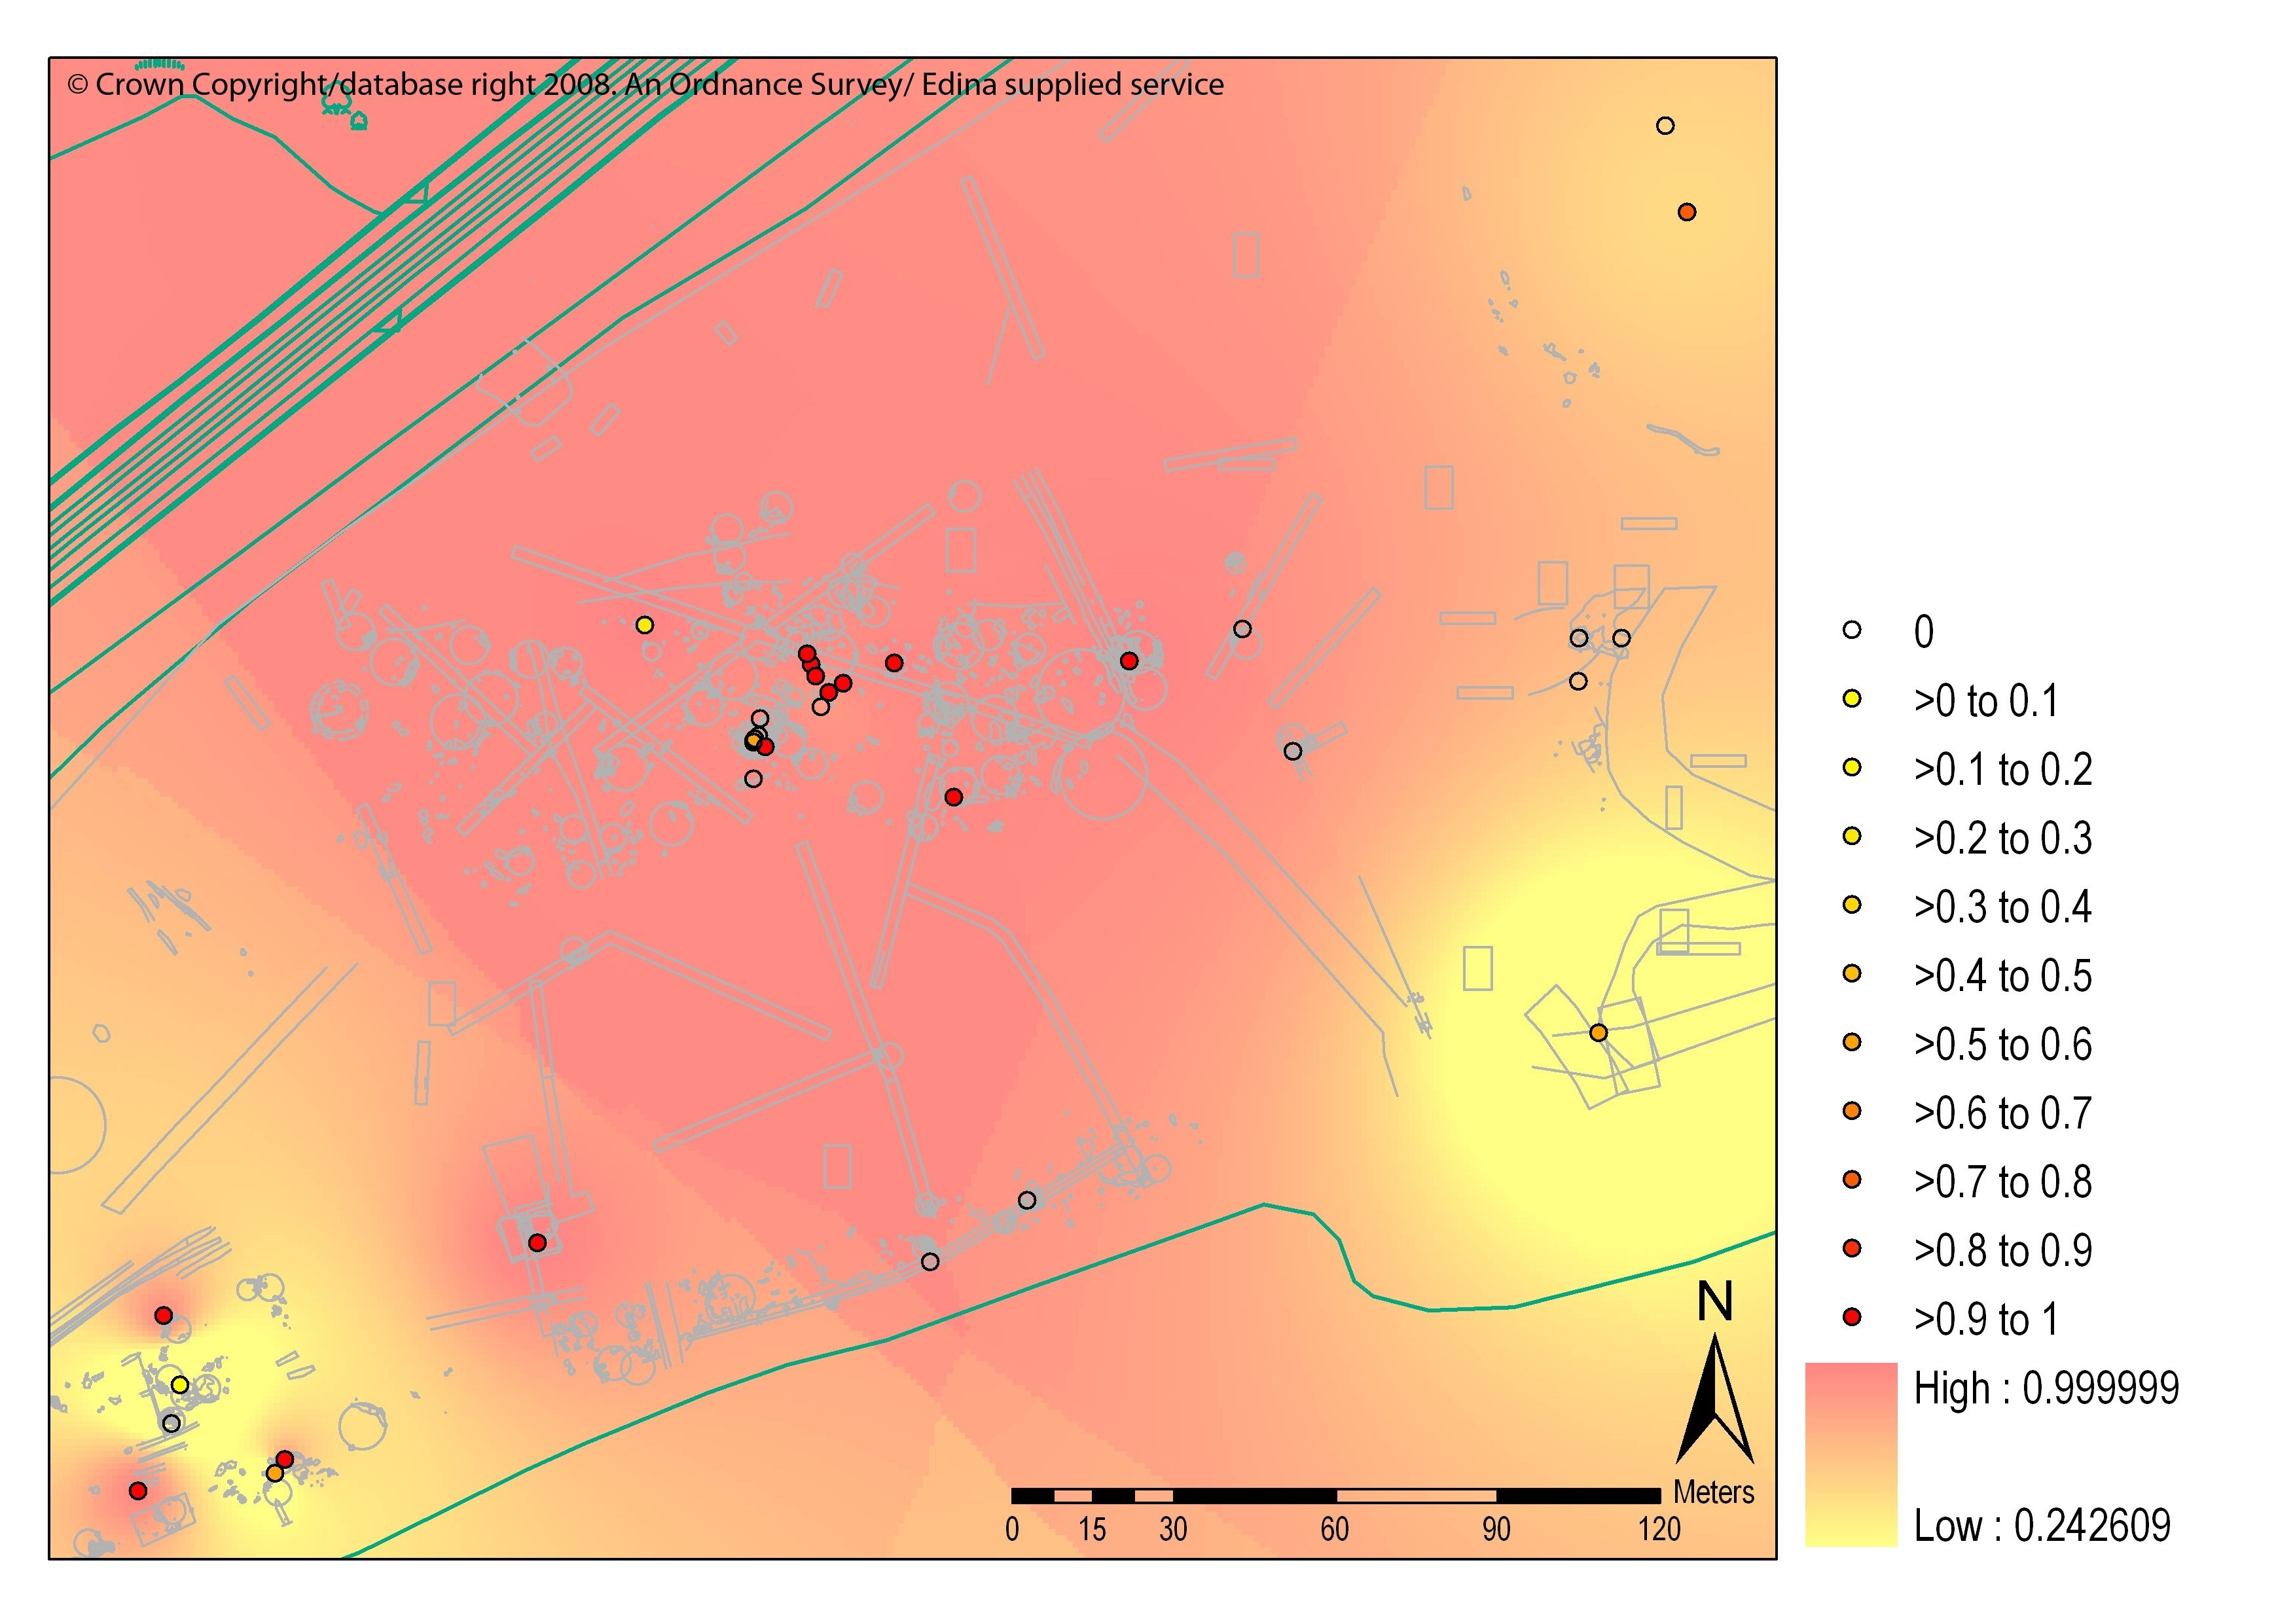
\includegraphics[width=0.9\textwidth,height=0.9\textheight,keepaspectratio=true]{figures/green2}
  \caption{Inverse distance weighted interpolation of bayesian probabilities: 3500-3000 cal BC, from \cite{Green:2008fk}}
  \label{fig:green2}
\end{figure}

Green's second use of interpolation, an inter-site case study, is effectively demonstrating the improvements in interpolating using his T-GIS, see figure~\ref{fig:green3} for an example output. However this still suffers from the problems with interpolations, including those that Green himself detailed. His crucial enhancement is that rather than points being assigned to specific phases, they instead have a probability function, which is used to determine the likelihood each point falls within a phase. This means that the data points can influence multiple phases and that in this case coarse ware pottery, which has more vague time spans, can be included alongside fine wares. He claims his method is an improvement on other similar approaches, such as aoristic analysis or p-use values, but provides no explanation or results to back this. In fact, the differences between his approach and an aoristic one are limited, with the time spans for each point in the interpolation split uniformly between phases just as in \citet[35]{Johnson:2004fk}. The difference is what happens next, Johnson sums the probabilities for each period to show how use changes over time (this description is truncated for brevity) in comparison to Green who interpolates for each phase, to show how such probabilities of use change spatially. Green claims that, unlike aoristic analysis, his method is ``not swamped by undiagnostic material'' \citep[224]{Green:2008fk} but does not back this up in any way. I would argue his approach is very similar to aoristic analysis, and his T-GIS could probably provide a convenient platform for performing it due to its discrete phase-based temporal model, and ability to split a probabilistic date into such phases. 

\begin{figure}
\centering
	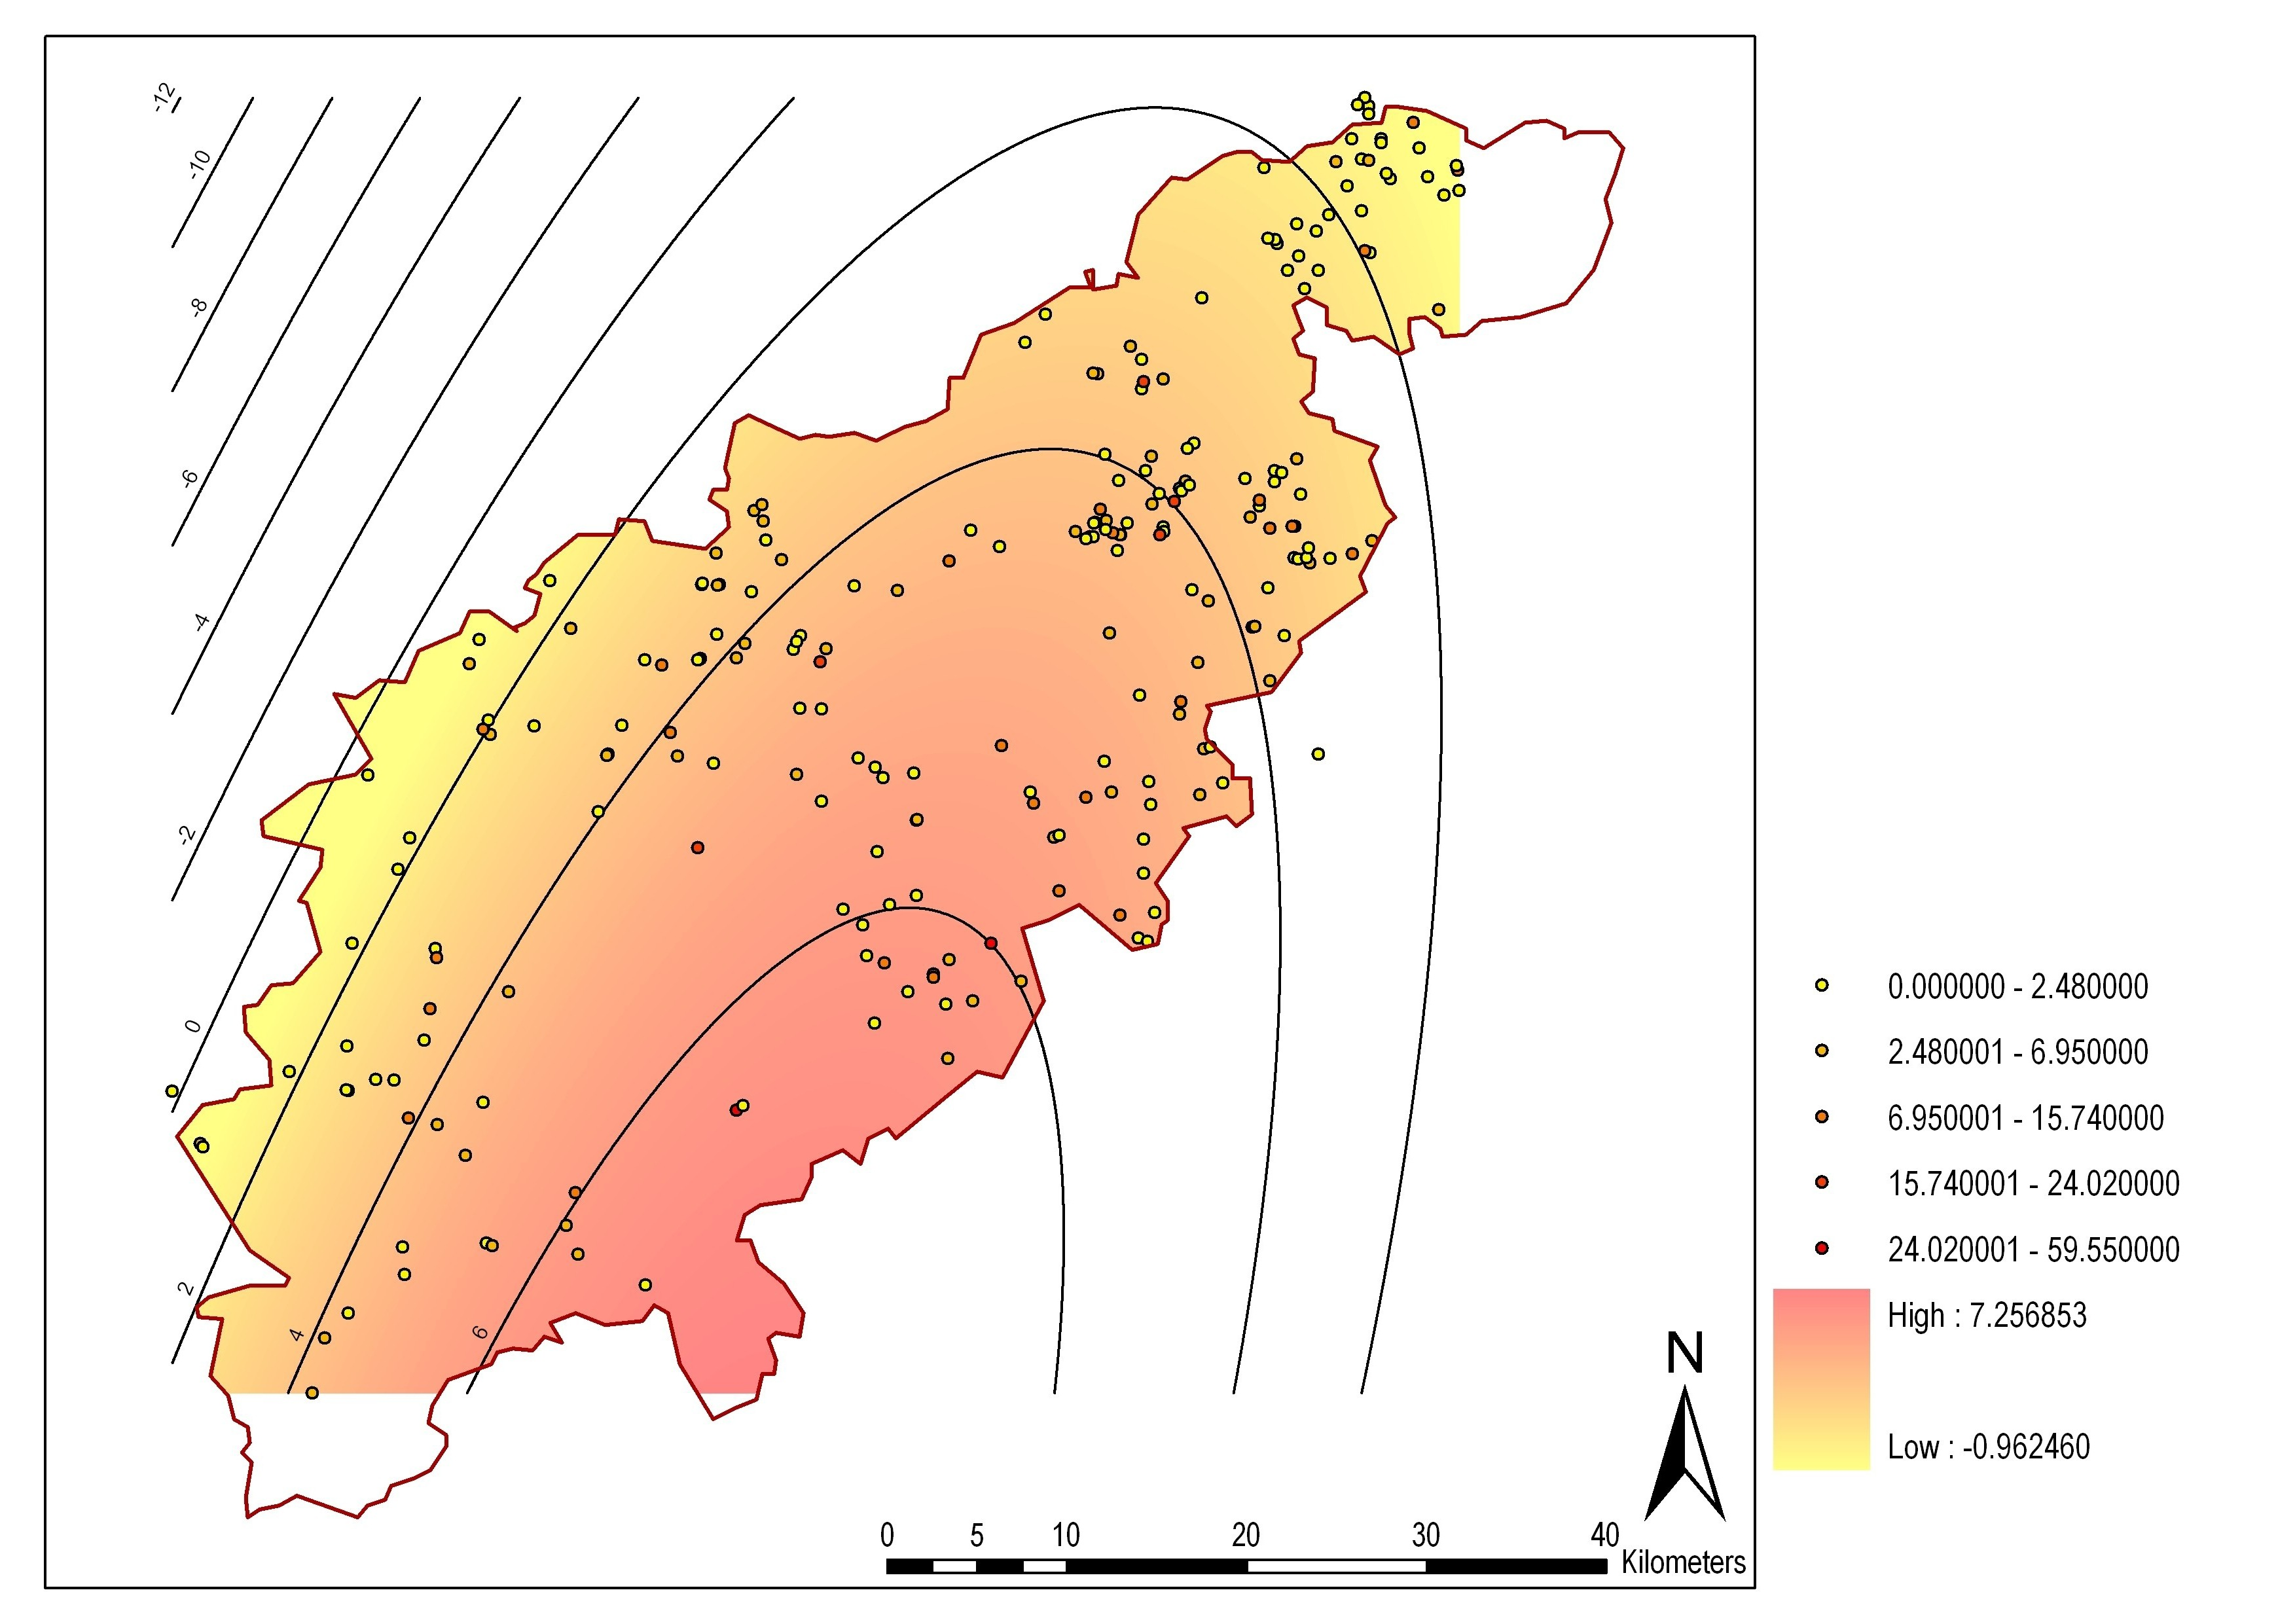
\includegraphics[width=0.9\textwidth,height=0.9\textheight,keepaspectratio=true]{figures/green3}
  \caption{Trend surface for Early phase (100 BC to AD 50) based upon TGIS probability output
normalised by sherd count. The point data layer shows the summed TGIS output, coloured from
yellow to red according to the parameter of summed probability multiplied by sherd count. The
trend surface is also shown in yellow to red, varying from low values to high, from \cite{Green:2008fk}}
  \label{fig:green3}
\end{figure}

Moving now to the tradition of spatio-temporal analysis outside of T-GIS, Johnson's introduction of aoristic analysis to archaeology \citep{Johnson:2004fk} has been noted. Specifically, as a method of analysing temporal data based on time-slices, rather than arbitrary periods and using probabilistic methods to account for the inherent uncertainty in most archaeological dates. The `aoristic weights' are ``often used as a proxy for evaluating change in the total counts of events across time'' \citep[448]{Crema2012}. Johnson made some changes to the method, which he called standardised aoristic weights, that correct for fact that modern artefacts could be assigned to individual phases with a probability close to one, whereas Palaeolithic artefacts would be assigned across so many phases they might only contribute 0.1 to each. \citet{Crema20101118} describe the peaks in aoristic weights as ``clusters of `high' knowledge'' \citep[1121]{Crema20101118} although, as they could be the result of a large quantity of data points of low probability values, the accuracy of that statement depends on what is meant by the term `high' knowledge. Does one actually know anything more about such periods than those which have a small number of data points with higher probability values? \citet{Crema2012,Crema20101118} augmented the ``vanilla'' aoristic approach by using the aoristic weights to determine whether to include a data point in a monte-carlo simulation, with \citet{Baxter2016120} providing more formalism to model generation. The resulting hypothetical spatio-temporal patterns were then analysed to determine if there was clustering in the pattern, \citep[1122]{Crema20101118} or if there was a significant change in the value of the modelled variable \citep[452]{Crema2012}. The clustering was categorised into three categories, these outcomes were then turned into percentages, and finally the probability for each cluster category. The concern with this approach is the cumulating uncertainty, starting with the original dating, then the aoristic value, next the simulations, which must include a degree of uncertainty and finally the reported probability of clustering. While there are a large number of simulations, they are only as valid as the aoristic analysis and original dating. There is also no probability attached to each simulation, some will be more likely if they include many features which have a greater likelihood of occurring in that time step. The resulting probability of clustering is based on the number of such simulations that have a clustered pattern of data.

 \citet{Crema2012} attempted to factor in the randomness derived from the monte-carlo simulation, by also computing a simulation where all of the events span the whole time frame (still with a uniform distribution) \citep[452]{Crema2012}. The rates of changes from this simulation are used as baseline of randomness from the simulation and only changes that are greater than this baseline are treated as a pattern in the underlying data. While this is a reasonable precaution, it raises two issues. Firstly, an acceptance by \citet{Crema2012} that the monte-carlo simulation will create additional uncertainty in the output and secondly by filtering it out in such a way only large changes were displayed, this meant they had to conclude that ``the outcome of the analysis did not point out radically new trends'' \citep[458]{Crema2012}. At best, their method was only able to suggest the potential for increases or decreases, but was not able to suggest numbers with any confidence, or even with an attached probability. This means it cannot really suggest the magnitude of increase or decrease and it is only capable of reliably reporting on larger changes. Surely the aim should be to refine data (as in bayesian modelling) not to make it more vague?

Fundamentally the problem with this method stems from its premise to ``identify novel patterns that are otherwise undetectable with traditional methods due to their coarse chronological resolution'' \citep[1125]{Crema20101118}. By trying to tease additional details out of probabilistic data, which only exist as an uncertainty, there is a real risk of treating the probabilities as pragmatic certainties when in fact they may not be so at all. It is perhaps more important to work with the probabilities, rather than trying to find information, which might not be there and is just a mathematical mirage.

The combined aoristic and monte-carlo approach as demonstrated by \citet{Crema20101118,Crema2012} has been taken up by other authors and adapted, for other spatio-temporal analysis. For example, land use has been investigated using this approach by \citet{ARCM:ARCM12182}. In this case, the temporal uncertainty was dealt with via simulation, during each simulation each archaeological feature was given a random date in its life span \citet[6]{ARCM:ARCM12182} - effectively modelling a uniform probability. Likelihood of an area being in use was the proportion of simulation runs that showed the area in use during a specific time slot, these were then interpolated to create iso lines of occupancy likelihood across the area being studied. In addition, categories were applied to each site, so that probabilities for use can be filtered by category, contour maps were created by category as well.

Other novel spatio-temporal methods have attempted to analyse changes in land use patterns by taking locations that are in use at a known time and then interpolating with that data to create contours of use, where the contours mark the probability of an area being in use at a specified time. This is the approach taken by \citet{ARCM:ARCM578} who use a kernel density estimate of spatial location to account for the fact that much archaeological material remains undiscovered \citep[1014]{ARCM:ARCM578} and a different kernel density estimate approach for the temporal data, which also averages out radiocarbon determinations as sites may have different numbers of radiocarbon dates \citep[1019]{ARCM:ARCM578}. Unusually, this approach formally deals with both temporal and spatial uncertainty in archaeological data to provide a model for showing changing land use in an area. The results are a series of contour diagrams, taken at 1000-year intervals. These diagrams show the effective spatial clusters created by the kernel density estimate, for each time slice. While the use of spatio-temporal probabilities is of significant value, creating spatial clusters in this way is of limited use. Take, for example, figure~\ref{fig:kde} which contains six active sites, in three groups, of two sites. Two sites form the basis for two of the clusters with another two sites broadly in between and one is pulled into the outer contours of one of the clusters. The diagram does not indicate what basis the central two sites do not form their own cluster, it is perhaps down to the weight of the temporal evidence. Alternatively, it may be an artefact of the algorithm, attempting to create the smallest number of clusters. In addition, the resulting land use values do not take into account the landscape over which they are draped (apart from excluding the sea) so areas of the landscape that may have geographical reasons for making them unusable (such as rivers, cliffs, etc) are smoothed out by the algorithm. There is little discussion or investigation of potential causes for areas to be used more during certain periods and also little discussion of the reasons or processes for that use to change, perhaps this is left for further work. 

\begin{figure}
\centering
	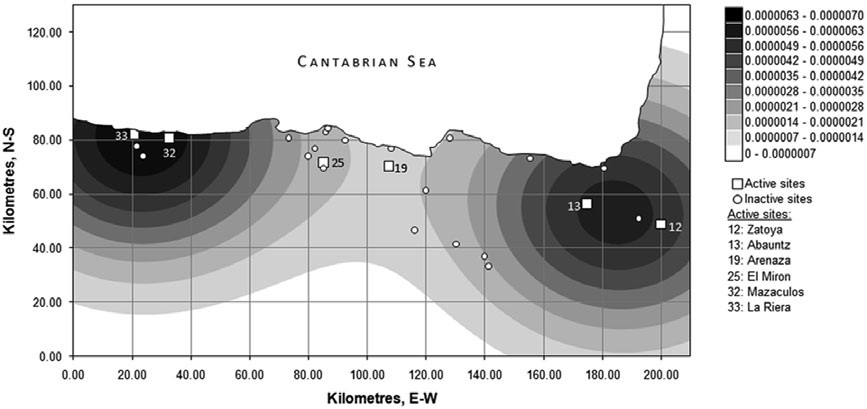
\includegraphics[width=0.9\textwidth,height=0.9\textheight,keepaspectratio=true]{figures/kde-plot}
  \caption{A bivariate KDE plot. Contour lines divide the
complete distribution into ten equally sized divisions per figure to indicate predicted density of population. Reproduced from \citet[1024]{ARCM:ARCM578}}
  \label{fig:kde}
\end{figure}

\citet{Demjn2016100} note that all of these approaches to spatio-temporal analysis are about quantifying past human activity, which is used to suggest intensity of activity, or by some authors as a direct proxy to population size \citep[100]{Demjn2016100}. Instead, \citet{Demjn2016100} set out to prove the link that ``variations in spatio-temporal distribution of archaeological settlement evidence mirror changes of settlement patterns'' \citep[102]{Demjn2016100}. Unlike previous work they first tested the mathematical model used to create the spatio-temporal distribution against simulated data to prove its validity, determine for what levels of site resolution it was valid, and compare to other methods, such as those by \citet{ARCM:ARCM578} and summed radiocarbon techniques. Their method relies on several unstated assumptions:
\begin{enumerate}
\item The mathematical model is valid;
\item Chosen model parameters are meaningful;
\item Variable feature visibility due to cultural behaviour has been ruled out.
\end{enumerate}

Point one is obvious, however the mathematical model presented by \citet{Demjn2016100} uses formulae that assumes the site and the archaeological activity are cylindrical in nature, such as that for calculating the intersection of two disks \citep[103]{Demjn2016100}. There is also the inclusion in the formula for the expected half-life of a site, although, nothing to suggest that archaeological sites have such a value in practice. Finally, this model has many similarities to the p-use representation of spatio-temporal data by \citet{Lock:1997vn} although they presented no formal method for computing activity. For point two, the model parameters for expected site radius and duration are somewhat arbitrary, with the site radius chosen as ``the average area of 20 ha (an estimation of an average prehistoric village and its immediate economic/agricultural hinterland'' \citep[104]{Demjn2016100}. Clearly this is only valid in certain locations at specific times, and would require replacing to use the model in other areas (or at least justification for retaining the same value) this is not a problem per se, but it does appear to be a very broad average which surely must hide significant variation across space and time. Point three is included by the authors themselves, ``if we are able to rule out effects of altered visibility due to cultural behaviour, the detected fluctuations can be interpreted as variations in actual settlement patterns'' \citep[106]{Demjn2016100} this is a big if, and is not addressed by the authors. It remains to be proved that it is possible to rule out these effects and until then, the usefulness of this approach is debatable.

Spatio-temporal analytical methods are varied, so far relatively under used and certainly under evaluated. The notion of additional information being present in radiocarbon distributions appears to have been adopted from more temporal studies, with the methods used to extract this hidden information becoming increasingly involved. Clearly a critical evaluation of methods is required before their results can be readily adopted, as has happened with bayesian modelling. This evaluation has taken a broad, rather than a forensic look at a range of methods that might be helpful in answering the kind of questions examined in the last chapter. Many methods have either methodological issues or complexities with their application. Fundamentally, as \citet{Torfing2015203} noted it is important to consider how the data we have relate to the questions we wish to answer and to pick an appropriate method based on this. 

\section{Alternative Approaches to Spatio-temporal Analysis}
This chapter has reviewed a wide range of quantitative analysis, starting with a brief review of spatial methods, a detailed examination of the two most prominent temporal techniques, followed by a review of the limited spatio-temporal methods available. The observation on spatio-temporal techniques by \citet{Demjn2016100} that most, if not all current methods focus on quantifying the intensity of past human activity is crucial, such methods are likely to easily fall foul of the issues identified by \citet{Torfing2015193}. Specifically any attempt at analysing activity must make assumptions to do with how archaeological material relates to ``activity'' (or population) it must then account for changes to the archaeological material post deposition and how archaeological recovery might affect patterns in the data. To dismiss such a line of research in its entirety at this stage would clearly be an over reaction, but surely there are also plenty of opportunities for a more contextualised school of spatio-temporal analysis. Such a school could be based around taking existing temporal methodologies and either extending them or performing additional spatial analysis. A key benefit of this approach is the ability to adopt methods for working with different scales of archaeological data, as the opportunity presented by a site wide data set is clearly very different from that presented by a continental scale data set. In order to achieve the aims of this thesis, of re-combining spatial and temporal data for unified analysis and of pushing forward the boundaries of such study it will be essential to explore the possibility of spatio-temporal analysis using such varied data sets.

In order to effectively work with and perform analytical procedures on such data sets it is likely that specialist software will be required. The subject of Temporal GIS is clearly a potential source for such tools, a thorough examination of the development and use of these tools will be required to understand how they can be effectively utilised to extend existing temporal techniques to include spatial data. %8,000 #23,020
\chapter{Spatio-Temporal Software}  %7770
\label{ch:tgis}
\section{Approaches to Archaeological Temporal GIS}
To make the most of archaeological data it is necessary to ask questions that consider both the spatial and temporal dimensions. In order to answer such questions, appropriate analytical techniques are required, such as custom methods for extending temporal techniques to perform combined spatio-temporal analysis. The platform for performing such analysis will therefore need to work with combined spatio-temporal data, clearly an appropriate choice for such a platform is temporal GIS. There has been to date, as \citet{Green:2008fk} put it, only a niche interest from archaeologists into temporal geographic information systems, with perhaps as few as two generic pieces of software being created. This has not stopped archaeologists asking spatio-temporal questions and devising methods for analysis that incorporate temporal information, recent examples including \citet{Frachetti:2006fk}, \citet{Palmer:2006uq} and \citet{Whittle:2008fk}.

The first consideration of the topic was \citet{Castleford:1992fk} who provides an overview of the state of play in the early '90s, at the time other disciplines were seriously considering temporal GIS (TGIS), especially from a theoretical perspective, such as \citet{Langran:1992uq}. Castleford brought this together with temporal archaeological studies and more general philosophy of time to propose some of the choices that would have to be made for an archaeological TGIS. For example, deciding whether temporal models should be points or intervals, or whether temporal databases would be better as relation or object oriented. While he does not propose the details for a specific system, his examination of some of the issues has laid the groundwork for subsequent researchers to come along and attempt to solve those problems. At the time he suggested archaeologists should become involved with the technical people creating TGIS software, however while TGIS has become commonplace in some fields, there are few re-usable pieces of software for archaeology. 

Castleford's research was undertaken at a time when there was considerable interest in Temporal-GIS from a wide range of subjects. \citet{Langran:1992uq} provides a perspective from the geographers approach, starting with an overview of the subject, an examination of what she calls ``cartographic time''  \cite[27]{Langran:1992uq} i.e. time as it is represented in a TGIS. This starts with a brief analysis of time from a philosophical perspective, however Langran quickly pushes this to one side in order to progress with the more pragmatic question of time in cartography. Unfortunately for archaeologists, Langran's cartographic time is precise and the temporal model has a fine granularity. This means that it is of limited use, as archaeological dates are often probabilistic and an additional source of temporal information is from the topological relationship between features. 

What is more useful for archaeologists is the more general information about the capabilities and requirements of a TGIS, for example \citet{Langran:1992uq} lists six major TGIS functions as: Inventory, Analysis, Updates, Quality Control, Scheduling and Display. This list is similar to that of \citet{Wheatley:2002ly}, with inventory being analogous to their spatial database. The main difference is the quality control and scheduling functions, which do not appear on the \citet{Wheatley:2002ly} list. 

\citet{Langran:1992uq} also lists the key technical requirements of a TGIS as:
\begin{itemize}
\item Conceptual model of spatial change
\item Treatment of aspatial attributes
\item Data-processing logistics
\item Spatio-temporal data access method
\item Efficient algorithms to operate on spatiotemporal data
\end{itemize}
The efficiency of algorithms is a significant part of her work, however it was written over 20 years ago, computing power and storage facilities have developed significantly since then. While these considerations are still very important, it is perhaps less crucial now than it was then. The other four technical requirements however are just as important.

In addition, Langran discusses some of the kinds of queries and operations that might be expected from a TGIS. This includes answering questions such as: where and when did change occur? What types of change occurred? What is the rate of change? What is the periodicity of change? It also includes assessing temporal data in order to determine whether temporal patterns exist, if so what trends are apparent and to try to determine what processes underlie the change.

These general requirements have formed a key part in many TGIS studies in archaeology since. However, it took several years before any follow up to Castleford's initial call to arms was made, the first being \citet{Daly:1999fk} who reviewed the progress on the study of time in archaeology since Castleford. They found that while there had been much work on the study of temporality in archaeology, there had been little progress on the implementation of TGIS. They discuss some of the issues faced by archaeologists in this area, and noted that there had been plenty of progress on the implementation of TGIS in other fields, in particular geography. They review several potential approaches to modelling time taken from geography, focusing on how relevant such approaches might be to archaeological applications. Most approaches suffer from the problem that while they may be able to show change, they do not necessarily help in analysing that change, for example in the snapshot approach where multiple raster's are stored as time slices, there is no actual information stored about the change, all it allows us to do is measure change by comparing values from different images \citep{Daly:1999fk}. The authors go on to suggest three potential methods for modelling and representing time which they think are suitable for archaeological applications: object-oriented database, animation and a z-axis. They note there are very few examples of object-oriented systems and the technical threshold is quite high, they are wary of animations due to the inherent lack of any analysis capability, which being key to any GIS system leaves animation more as a form of potential output, but not a temporal model. Their favoured approach is the z-axis, as used by many space-time geographers, a theoretical description of such a system for archaeological use is presented in \citet{lock2002analysing}, discussed below. \citet{Daly:1999fk} also offers up some of the potential uses for a TGIS, such as the ability to study how people in the past experienced and interacted with time. They suggest the time-space life worlds of time geographic research may be applicable to cultures and societies. This would make such techniques more practical for archaeological data, with the temporal rhythms of societies manifested in the spatial configuration of their activities \citep{Daly:1999fk}. While the article provides a valuable review of the literature as of 1998, it does not add any tangible technology, it does however provide a potential direction for the future of TGIS in archaeology.

\citet{Lock:1999fk} provides an interesting re-usable approach to studying time through GIS, while it  is not a packaged system, it does offer a method for including many of the features archaeologists might expect to find in such a system. The temporal model for this approach relies on pottery typology and quantitative data of pottery find distributions (i.e. from field walking) where different time periods are represented by different types of pottery. By splitting the finds for an area based on their type, they analyse how pottery deposition is different for each type, therefore how it changed over time and use this to infer a change in activity levels on a site over time. In its basic form this is done by subtracting the two quantities represented as raster images. This study takes that analysis a step further, using classification to aid visualisation and by suggesting two further methods, one for examining the change relatively, and the other for doing qualitative analysis. These extensions to the method can be used to account for the significance of different types of pottery, and the classification enables the use of contingency tables for further analysis. Clearly, this is a limited model, crucially reliant on pottery typologies, but its simplicity does enable the researcher looking at large areas to start to visualise how that area might have changed over time, identify the most profitable parts to investigate for a particular period, or to try to understand change between periods. By focusing on continuity or change the temporal model fits well into a raster based system, it can provide output that is clear and intuitive, however the low level of resolution has the potential for creating authoritative looking outputs that mask the true complexity of the underlying model, of the actions and events that led to each act of deposition. Using their suggested techniques for relative and qualitative comparisons would enable the archaeologist to control this to a degree, but not alleviate it entirely. 

The difficulties of visualising temporal data in GIS were carefully considered in \citet{lock2002analysing}. The approach they recommended was designed to break the constraints that they saw on the representation of change through time in 2/2.5D views. They argue that existing GIS systems lead to temporal data being simplified, as they cannot natively support a temporal dimension. Time is then often reduced to a specified span, or a period code for each feature, stored either as an attribute, or using temporally organised layers. This oversimplification is not only a reduction in the quality of data, but may also influence the study of change, for example with a focus on comparing characteristics of clearly defined periods that in reality are not so clearly defined \citep[4]{lock2002analysing}. With respect to visualisation, they are critical of using colour coding of sites to represent time, due to the potential for creating a complex mess of colours and for the problems of sites that span periods. The fundamental problem they see with these categorical techniques is that time is continuous, and therefore must be analysed as such.

The Temporal-GIS system they propose to account for these problems has never been created, so its efficacy in practice is unknown. It is fundamentally based on probabilities, enabling it to deal with the uncertainty of archaeological dating. The probabilities are called p(use) values, they represent the probability that a site was in use at a particular point in time. This allows archaeologists to easily model sites, which have a period of time in which they were definitely in use and the areas either side of this where they may have been in use. The p(use) values for a particular site are computed based on the p(use) values for each piece of evidence from that site, with the recommended approach being to take the greatest of all the values. The result being a p(use) timeline for the site, which is used for a 3D spatio-temporal representation. The p(use) values are defined by the archaeologist, enabling them to incorporate a range of knowledge about each piece of evidence. At first glance this is an attractive system, however, to approach a continuous z-axis would require an archaeologist to place a p(use) value on every piece of evidence for each site along the z-axis at a high enough resolution that meaningful analysis could be performed. The problem being that our knowledge of use may be highly discrete, we may have a very good idea of when something was in use, and when it was not in use, but very little detail on the transition. The solution is a continuous p(use) function, but there is no clear way of providing this for a variety of different evidence types, such as radiocarbon, pottery typology and site morphology. In addition, with such a breadth of potential evidence being one of the stated benefits of this method, to focus on one type of dating evidence alone would severely impact its usefulness. There is also a further problem to placing all the p(use) values at the archaeologists' discretion, that of lack of rigour. Without a system or framework for computing such values, it is more difficult to argue about how they have been reached and very easy to argue about the values themselves. 

One of the fundamental goals from \citet{lock2002analysing} was a means for visualising temporal data. Even if there are problems with the underlying temporal model, the visual aspects to their approach have their own merits. As an intuitive display of temporal data a 3D approach with continuous z-axis is very appealing, as they note it has the potential for using topology to explore spatio-temporal patterns and for performing analysis of temporal data \citep[5]{lock2002analysing}. There are a couple of concerns with this approach, firstly, in a crowded landscape viewing 3D representations on a screen could prove very tricky, in particular it will be difficult see sites that are both near and ones that are further away from the origin at the same time. This could potentially result in sites in a part of the landscape at one point in time appearing to be spatially much nearer to sites in another part, further along the y axis, at a different point in time. There is also the issue of probability, this means that the temporal relationships between sites will likely also have a probabilistic nature, so too will any analysis along the z-axis. The result of these issues is that, at best, it is going to be very easy to get undecipherable screens, and depending on the allocation of p(use) values users may end up with ``garbage in - pretty maps out'' \citep[1]{lock2002analysing}.

Following this, \citet{Ceccarelli:2003fk} attempted to construct a spatio-temporal GIS to model landscape change, focusing on the area around a lake in Tuscany. Their solution involved a time database combined with spatial modelling, using animation to represent time as a third dimension for output. However, the changes to the shoreline are not visualised in the animation as a continuous change, but as four distinct  versions of the coastline, shown in sequence. Within their database, this makes sense, as they treated time as a categorical value, the different visualisations of the landscape presumably corresponding to one or more categories. It is curious that they have then created an animation, with a continuous time variable, and as \citet{Green:2008fk} notes, it is a bit deceptive. It would appear that by using a long list of software they have created a visually appealing animation displaying multiple layers from a GIS sequentially, where the layers show the same landscape at different points in time, and contain key archaeological and historical information overlaid. As with other systems a large focus was on creating a means of representing change through time to the public in an easily consumable fashion, rather than performing any kind of temporal analysis. This project was also a very bespoke solution, using lots of software, including: AutoCAD, Access, ArcGIS, Grass, PostgreSQL, RDBMS, 3D Studio Max and QuickTime. It was by no means re-usable temporal GIS software.

\section{Temporal GIS Implementations}
\citet{Johnson:1999cr} was the first attempt at creating a distinct archaeological temporal geographic information system, the TimeMap project. The TimeMap software created for the project has been very successful; it was used in the Museum of Sydney for a kiosk application, the Electronic Cultural Atlas Initiative, and as a map interface for educational software MacquarieNet \citep{Johnson:2002kx}. However, it hasn't been used in many archaeological projects, despite the lack of TGIS for archaeological uses being one of the key drivers behind creating the software. Green neatly summarises the situation ``TimeMap's greatest successes have been in areas outside of core TGIS issues for archaeologists and whilst using non-archaeological data'' \citep[101]{Green:2008fk}. The reason for this is down to the initial objectives. In fact, there was no specific target application in mind \citep{Johnson:1999cr} and this has allowed the project to be pulled off course. \citet{Johnson:1999cr} explores the subject of archaeological TGIS and defines some distinct requirements for such a system, including the ability to deal with uncertainty in temporal data, he also defines the temporal model to be used - the snapshot-transition model. The first projects the TimeMap software was used for are the mapping of Asian empires and Historic Sydney \citep{Johnson:1999cr}. While neither is a strictly archaeological project, there is potential for the inclusion of archaeological data. TimeMap seems to have changed direction by \citet{Johnson:2002kx}, as there is much less focus on Archaeology and the issues around archaeological TGIS, but much more focus on education and interactive mapping as an educational tool. This is exemplified with the change in focus of the projects now involved with TimeMap, to museum and education applications. This shift was accompanied by an increasing focus on the use of the web, the networking capabilities became a much more important part of TimeMap, but are hardly essential for an archaeological TGIS. 

In terms of its use as an archaeological TGIS TimeMap suffers from a number of problems, its snapshot-transition model does not record the topological relationship between features \citep{Johnson:1999cr}. This is a key form of temporal relationship in archaeological data. Another important format of temporal data in archaeology is the probabilistic, such as radiocarbon dates, while \citet{Johnson:1999cr} discusses the importance of fuzzy dates and a mechanism for coping with them, there is no indication of applying the technique to probabilistic dates. Without support for topological or probabilistic dates, TimeMap's use within archaeology is quite limited. Presumably this is why the datasets that have been used are all of a historical nature, they can provide exact dates down to specific years, which is also much easier to represent. \citet{Johnson:2002kx} presents the space-time cube as the ultimate representation of spatio-temporal data. The space-time cube depicts accurate and exact information, however to represent a probabilistic date in this way could easily imbue it with a false accuracy or exactness. With hindsight there are many issues with the project, but TimeMap was the first bespoke ``archaeological'' TGIS, to create it meant finding answers, or at least pragmatic solutions to some of the problems for which earlier authors had only hypothesised solutions. It has laid the foundation for subsequent work in archaeological Temporal GIS, primarily \citet{Green:2008fk}. 

\citet{Green:2008fk} has moved the discipline a significant step closer to an archaeological temporal GIS. It can be seen as a proof of concept for the technique of providing bespoke archaeological temporal facilities within ArcGIS and demonstrates the potential for TGIS studies in archaeology. The thesis starts with a comprehensive review across the literature, from philosophy of time, through archaeological theory, the study of time, to digital archaeology and the history of the study of temporal GIS in archaeology. The only notable exception being the use of GIS in archaeology. The software created by Green is a plug-in for ArcGIS, which he describes as a ``fuzzy temporal GIS'' \citep[242]{Green:2008fk}. 

The primary function of the software is to compute the probability that a date, or set of dates fall within a defined time span, as such it only deals with absolute dates, it does not consider relative dates. These probabilities can then be drawn in ArcGIS using the spatial co-ordinates of the dated object, with the probability value represented on screen using a mechanism, such as colour, to indicate the likelihood it falls into the time span. In practice Green used several time spans for each of his case studies, where a time span represents a period that the archaeologist wishes to analyse (e.g. Late Neolithic) this results in a series of outputs for each site, presenting a set of snapshots visualising the probabilities that the mapped dates occur in each time span, figure~\ref{fig:green1} is an example of such a snapshot. There is no indication whether the dates are more likely to have occurred during a particular part of the time span, so in many ways the result is not too dissimilar from a snapshot model, there is also no information about the transitions between each phase, or time span. Unlike the snapshot model, output can be generated for any time span without the need for interpolation. With large datasets these outputs quickly become messy, with coloured points overlaying each other. For his first case study, the intra-site example, points were overlaid on a base map containing features from multiple periods, utilising the same base map for each run of the system, even though each run represented a consecutive period. The resulting output retained eligibility only due to the sparseness of the temporal data set. There is also no relationship in the system between the dates, represented as points, and the features. The lack of a clear operational model to Green's TGIS is a big omission, without encapsulating change in the system its effectiveness is very limited. As a conceptual model of change is one of Langran's key technical requirements of a TGIS, this does raise the question of whether it is indeed a TGIS at all.

Data is input by augmenting the shapefile containing point data, so that each entry also contains a minimum and a maximum date as attributes, apart from OxCal data, which is contained in a separate table, linked to the shapefile within ArcGIS. This is a convenient method of getting temporal data into ArcGIS, but Green's labelling it as the temporal model for the system is unconvincing. The temporal model that is encapsulated in this system clearly draws on the B-series notion of time as it deals with dates BC/AD or BP. The minimum and maximum dates specified are used to define a period during which the date occurred, rather than a beginning and end date for the object or event. It is also not clear what dates in the data model represent; when radiocarbon dates are used, they represent a specific event causing the sample to cease its exchange of Carbon, whereas dates from other sources may have different meanings. Surely, an important element of the temporal model is what the dates actually represent. Another issue with the data model is that it only deals with point dates, so it cannot consider the life of an object, it is in effect a one dimensional temporality, one that does not store change, or life spans. 

The TGIS of \citet{Green:2008fk} had one primary form of analysis, the calculation of probabilities that the temporal entities within the system fell into a user specified date range. In his case studies this was then used as the basis for colour coding the plotted data. It also provides several secondary analysis methods, which are not applicable to the main data type, radiocarbon dates, as they involve summing probabilities.

These analytical methods are solely focused on the temporal data, with the primary function, computing probability, creating secendary data that can lead into further spatio-temporal analysis. The use of interpolation is problematic, Green notes many problems himself \citep[189]{Green:2008fk} especially for sparse datasets, such as his radiocarbon dataset. Fundamentally though, it is essential to consider the underling assumptions the interpolation is based on, that locations closer to certain dates are more likely to have dates closer to that date than ones further away. The results of interpolation like this are attempting to show the spatial distribution of the probability that dates occurred during a specific time interval, i.e. the likely focus of dated material during that time interval. However with a sparse data set, likely to have been heavily influenced by post depositional processes, considered across a relatively small scale area, the underlying assumptions of the use interpolation is, perhaps questionable and the generated probabilities could just as easily reflect the likelihood of finding material as identifying areas of focus of past activities. Clearly spatio-temporal interpolation is a tempting analytical method, as Green uses it twice, however it must be treated with caution. Green's second use of interpolation, \citet[206]{Green:2008fk} based on pottery data is performed with a clear question in mind and provides a much more robust set of results. It is also over a much larger area and is looking for a more general trend. By using trend surface analysis Green demonstrated broad trends in the distribution of different pottery that had similarities to earlier, conventional interpolations of pottery data. With a large data set, over the area of a county this can demonstrate clear areas of focus during particular periods. However there is still a very basic problem, that if a large part of the area has dates that have a broad potential range of possible dates, there will be minimal distinction between the different date ranges. 

Despite its limitations, \citet{Green:2008fk} is a watershed moment, from research that is mostly about how we might do T-GIS to actually writing bespoke software. In addition, he was able to demonstrate its usefulness in two very different contexts. Crucially he was able to combine the statistical, technical, almost processual approach to data, with the kind of post processual theory and analysis that leads to an evidence based humanising of people in the past.

\section{Next steps for Archaeological Temporal GIS}
There is clearly a gulf between the theory of archaeological T-GIS and the implementation. Moreover, implementations that are less driven by the archaeology, such as TimeMap, ultimately end up being much less useful for archaeologists. This is perhaps mostly due to the disconnect between T-GIS theory and the spatio-temporal data available to archaeologists, as a large part of the founding theory has been written by geographers. The other disconnect between theory and application, as exemplified by \citet{lock2002analysing} is that while it is important to consider temporal models and ideal ways of representing probabilistic spatio-temporal information, it is an entirely different thing to implement those models and render the output. To bridge this gulf, pragmatism is clearly essential, only heeding those aspects of T-GIS theory that are applicable to archaeological applications and data. 

This pragmatism has so far been best demonstrated by \citet{Green:2008fk} in his use of the ArcGIS platform, while this comes with being limited to the ArcGIS SDK, in practice that is not particularly restrictive and it provides access to a mature GIS environment. Despite nearly 25 years since the first interest from the archaeological sector, the use of T-GIS in archaeology is still in its infancy, a fully featured platform is a long way off. At the moment archaeological T-GIS are single use applications, providing a subset of available analytical methods to answer specific questions, although the list of true spatio-temporal methods is itself very limited at present. Over time, more methods will be added to the list, so that we will one day be in a position to build an environment that can handle archaeological spatio-temporal data and perform a wide range of useful analysis.

Having reviewed the available T-GIS created within archaeology, it is clear there are non that are capable of performing the kinds of analysis required to enhance the field of spatio-temporal analysis, specifically by incorporating spatial data into temporal analysis. Instead it will be necessary to create bespoke approaches to answering individual questions, with such approaches incorporation a subset of T-GIS capabilities that are necessary to perform a particular analysis. At this stage too much focus on re-usable systems is not particularly helpful, instead, a focus now on spatio-temporal questions and spatio-temporal methods will be crucial in defining the T-GIS of the future. 

\section{Essential Temporal GIS Components}
There are several components of T-GIS systems that will be necessary for performing any combined spatio-temporal analysis, however they can be tailored to the specific methods and therefore be considerably less complex than those required for general T-GIS applications.

\subsection{Spatio-temporal Model}
The spatial model used by typical GIS systems is essentially one of cartesian space. In order to model the world more accurately, layers will have various projections onto this space so that they can represent what is on the ground. Ultimately the GIS deals with co-ordinates, often 2D, sometimes in 3D. This is very much along the lines of the absolute concept, where space is a container of objects \citep{James-Conolly:2006qf} or perhaps in some ways analogous to the B-series notion of time. Such an objective model of the world is important in that it allows the combination of data from disparate sources in such a way that it is easy to view everything related to a specific area, even if that information comes from a variety of data sources. It is also the view of the world that most forms of cartography use, meaning that maps and surveys fit straightforwardly into GIS.

Just as the A-series is the subjective counterpart in terms of time, the relative concept of space makes it an attribute of objects, events or people \citep{James-Conolly:2006qf}. From this perspective it is possible to examine how people understand the space around them, ask questions of being-in-the-world and of the experiential nature of space. This is an area that modern GIS studies in archaeology have started to tackle. Crucially it has been possible to ask questions about experience and perception from within a GIS where the underlying spatial model is absolute.

There is no reason why this same approach cannot be taken with time, \citet{Green:2008fk} makes use of absolute dates as the basis for his temporal model. One of the objectives of the T-GIS then becomes providing a framework for analysing time as experienced. The same approach was taken by \citet{Johnson:1999cr} in TimeMap and also the continuous z-axis of \citet{lock2002analysing}. In fact there are few examples that do not use absolute dates, as these are one of the most readily available to archaeologists.

By taking this approach to time it is important not to assume that it is theoretically neutral, in the past GIS was considered as such, however it has been demonstrated that this is in fact not the case \citep{Wheatley:1993qf}. So far, the theoretical nature of time has revolved around splitting time along the lines of the A/B series theory of time as adapted by \citet{Gell:1992fk}, in particular with his adaptation of Husserl's model of Time-consciousness. On this basis, to attempt to understand how people in the past understood time we must consider the A-series. \citet{Green:2008fk} drew a connection between Husserls ideas of reproduction, retention and protection with the broad themes from \citet{Bradley:2002fk} of people in the past looking into their distant past, their immediate past, looking towards the future and people in the past encountering ancient remains. 

There are many other theoretical approaches to time, even though the A/B series sits neatly alongside the predominant spatial model it is worth considering other approaches as they may have valuable insights for the temporal model.

The Annales school approach to time could be applicable to a TGIS approach, with the individual dates being stored in the temporal database representing short term events. The challenge is to knit these into longer term discourses and explore the longer term process behind the short term events. This in some ways parallels archaeological interpretation, the objects found and dates associated with them are of events taking place in the short term. However the understanding of past societies, process and cultures will take place over a longer time frame. Such an approach could favour the representation of changes to society as happening over the long term, when in fact this may not have been the case. Instead non-linear systems could provide a model for more sudden, dramatic change. Potentially this could fit well with the tighter date ranges yielded by bayesian modelling of radiocarbon dates.  Coming from a different theoretical standpoint, time-geography may have some difficulties with the types of data archaeologists have available, for example constructing a time budget is much more challenging as there is little insight into the lives of particular individuals. However the more general ideals of taking social ideas and representing them in physicalist terms could hold potential, perhaps as a method of visualising archaeological assumptions. Such a temporal model would probably have to be quite advanced, but if achievable might yield interesting results when combined with biographical approaches. Another theoretical model of time is time economics and opportunity costs. In the post-processual world of modern archaeology such an approach could be divisive, but could yield interesting results about the way people in the past made use of their time. With models and simulations of opportunity costs it would fit well into GIS analysis. 

Clearly there is a wide variety of potential influences from which to draw for the spatio-temporal model. The specific theoretical foundations will depend upon the analytical method used and the ultimate questions that are being addressed. The broadest theoretical approach would appear to be the A/B-series as advocated by \citet{Gell:1992fk}, which will work well with existing spatial models. The Annales school and non-linear dynamics both incorporate the idea of different scales of time, and focus on change. The representation of change is referred to in \citet{Castleford:1992fk} as the operational model of the TGIS.

\subsection{Operational Model}
\citet{Langran:1992uq} suggests several conceptual models of time: space-time cube, sequential snapshots, base state with amendments, space-time composite. Of these approaches, Langran favoured the space-time composite, while \citet{Johnson:1999cr} chose sequential snapshots, and the z-axis approach of \citet{lock2002analysing} is a derivation of the space-time cube, that allows for probabilistic dates. 

The space-time cube is perhaps the most visually appealing, with ``the trajectory of a two-dimensional object through time create[ing] a worm-like pattern in this phase space'' \cite[37]{Langran:1992uq} however as \citet{lock2002analysing} noted there are problems with the uncertain nature of archaeological data. Langran also notes technical and conceptual problems with this approach, especially with large data sets and the representation of change. This is of critical concern to an archaeological system and there are multiple options, for example, does it interpolate between known data or instead represent change in a stepwise fashion \citep{Langran:1992uq}? \citet{lock2002analysing} suggest a way of displaying uncertainty, and their p-use values effectively provide a mechanism for manual interpolation of change.

The sequent snapshot approach is analogous to a set of maps with each time slice being a different map in the sequence \citep{Langran:1992uq}. For Langran, the problem with this model is that the snapshot represent states, but they do not represent the events that capture the change. In order to determine change the snapshots must be thoroughly compared \citep{Langran:1992uq}. The snapshot-transition model used by Johnson is similar to this, but as well as the snapshots, it also stores information about how to transition between snapshots. Crucially interpolation is required to visualise a state that is not the exact one recorded by a snapshot. 

Base state with amendments provides a much more efficient means of storing temporal data, with change explicitly encapsulated in the amendments \citep{Langran:1992uq}. It is possible to move individual objects forwards and backwards in time, and to analyse the mutations between the amendments. There are no archaeological implementations of this model.

The space-time composite is in many respects an extension of the base state with amendments model except that rather than image overlays, the amendments become new objects in the system, where each object has its own attribute history, represented by an ordered list of records \citep{Langran:1992uq}. Langran details how such a system could be implemented, yet so far no archaeological examples have been constructed, despite the detailed instructions. This is perhaps due to the inexact and incomplete nature of archaeological data, we may have information about a change, but it may be only partial information with a probabilistic date, where as the space-time composite model relies on exactness.

According to Johnson the snapshot-transition model replicates our knowledge about the past \citep{Johnson:1999cr}, however \citet{Green:2008fk} disagrees, in its raw form he states that archaeological temporal data is point based and topology based. However Greens simplification disregards the fact that, ultimately a dated sample represents an event, something that happened to an object (e.g. burning) and that object has a physical manifestation, one that forms a part of the topology of the site. The event represents a change, one which may also be represented in the chronology of the site. In fact the topology of the site is a record of the changes that have occurred, this view of change is in many ways similar to that of \citet{Ingold:1993zr} where the topology of features in the landscape is the physical manifestation of changes made to that landscape over time. 

However, taking a typical method of storing chronology, the Harris-Matrix, would only store the chronological events, it is an a-spatial model of change. Clearly this is only half the answer, and a TGIS must also be capable of storing spatial change as well. In many ways there are parallels to Langrans space-time composite, where space and time are stored separately in two databases \citep{Langran:1992uq}. Archaeologists most frequently represent spatial change with successive plans and diagrams, so it also makes sense to follow Langran and store the chronology separately to the plan as the spatial data is best stored using conventional GIS formats. The two structures should be linked so that it is possible to model the changing spatial extent of a feature throughout its chronology. While there may be certain scenarios that would favour one form of operational model over another, the pragmatic approach is clearly to adopt a form of the space-time composite, with linked data stored in parallel, although not necessarily as a base state plus amendments model.

So far there has been a recurring theme of data, without a consideration of what form that data might take. Having considered spatio-temporal and operational models, it is important to consider what data will be available and how that can be stored in such a way as to realise these models.

\subsection{Data Model}
So far the loosely recommended approach is to use absolute dates for the spatio-temporal model, with a combination of chronology and plans comprising the operational model. There are a range of absolute dating methods available to archaeologists, the most frequently used method is undoubtably radiocarbon dating; the added complexity of radiocarbon dates is that they are in fact a probability. Related to this is their requirement for calibration. \citet{Green:2008fk} uses the OxCal method for storing calibrated dates, which splits the date up into a series of slices, storing the probability that the actual date falls into each slice. 

The chronology of a site could potentially be represented using one of several schemes, with the most common probably being the Harris-Matrix, from \citet{Harris:1989vn}. It has been shown that the Harris-Matrix can be efficiently and effectively stored and analysed digitally using a Directed Acyclic Graph (DAG) data structure \citep{Ryan:1988ly,Herzog:1991ve}. Another potential format would be the OxCal model used as input to the bayesian modelling algorithms, this would aid re-use of existing data and provides a clear connection between temporal and operational models. While both of these models encapsulate change, they embody a very different kind of change. Whereas the Harris-Matrix diagram is a representation of the physical stratigraphy, the OxCal model is a hypothetical model of the sequence of events. Effectively the OxCal model can be thought of as being at a greater level of abstraction than the Harris-Matrix, which is more at the coal face of the chronology. This is due to the interpretation of the site's chronology by the model builder, having translated the changes in features, in stratigraphy and phasing of the site into the abstract form of the OxCal model. Finally, let us consider the relationship between the chronological model and spatial features. For a Harris-Matrix the spatial data can be used to show changes in the physical objects represented in the model. The OxCal model does not represent physical objects, it represented events. It is these events which are the vehicle of physical changes, so in order to show change it would need plans of the actual changes to be linked to the events in the model.

\subsection{Generating Output}
The representation of temporal data and display of results from analysis of temporal data is a subject of its own right. While humans have an inherent visual understanding of space, the same is not necessarily true for time. Time can be represented as a clock or as a line, but there are inherent problems with such methods requiring high precision and being rigidly linked to modern clock time, or at least a B-series style temporal model. 

This has not put off \citet{lock2002analysing}, who suggest the use of 3-D structures such as voxels. They recommend their p(use) method to overcome the problem of uncertainty in archaeological data and the probabilistic nature of dates. This has been discussed previously, from a visualisation perspective the problem is with displaying a spatial entity that may or may not be present at a particular point in time, and representing that uncertainty. In the case of p(use) the absolute value of which should be represented in some way by the display, so elements with a high p(use) are obviously distinct to those with a low value. There is then the question of how to display changes in physical form, the uncertainty of when the change took place and also displaying changes to use. Part of the problem here is the assumption that a spatio-temporal GIS must surely have a method for visualising both time and space together, in some abstract, intuitive form. This is an unhelpful assumption, and just as GIS view space from a different perspective to the one we would experience it (with the omnipresent, God's eye view) there is no reason the same cannot be true of time. Such an abstraction from the human perception of space is often seen as a criticism, removing us from the world, however it is a convenient and often helpful way of viewing the world when performing spatial analysis.

In order to bring the viewer back into the world, virtual reality and animation are often employed to represent spatial data from the perspective of someone actually present in the landscape. In a similar way, several attempts have been made to use animation to represent time in an intuitive way, although spatially these have been from the top down perspective, they are similar in that they represent time as it is experienced, by its passage. This has been the favoured approach to representing time in TimeMap \citep{Johnson:2002kx} and also in \citet{Ceccarelli:2003fk}. While it has it admirers, animation suffers from a number of key problems, firstly it is not interactive, a user cannot perform selections or manipulate data, once in an animation, it is shut off from any further manipulation. Secondly it does not help with the issue of uncertainty in the archaeological data, while transitions can be created by fading features, this implies a certainty of a gradual change.

\citet{Green:2008fk} took a different approach, rather than creating a spatio-temporal display, he only visualises the probabilities that the TGIS produces. The temporal aspect is reflected in the parameters of the analysis and are therefore a static part of the resulting output. In other words the augmented shapefile that is the output to the system is a product of the date range used to work out the probability values, he then uses colour to visualise the probabilities created. \citet{Johnson:1999cr} refers to this as symbolism, one of four techniques he suggests for squeezing an extra dimension out of a computer screen, the others being time slices, arrows and difference maps, see figure~\ref{fig:time-maps}. In effect Green is mapping the variation of probability over space, using colour as an extra dimension (or half dimension) as the main axis are taken up by the spatial co-ordinates.

There are clearly a wide range of potential techniques for visualising spatio-temporal data. The applicability of a 3-D view to archaeological data is unconvincing, primarily due to the uncertainty of probabilistic dates, instead it is more important to focus effort on the analysis and providing a suitable means of representing those results. Animation would certainly help with tackling being-in-the-world issues and can provide an immersive experience, but it is not an analytical tool. One of the aims of outputs is clearly to display the available data, but as \citet{tufte1983visual} notes they also serve as ``instruments to help people reason about quantitative information'' \citep[91]{tufte1983visual}. However, he is also clear on the limitations of the passage of time as a form of causal explanation, \citep[37]{tufte1983visual} suggesting that any diagrams displaying time should only do so as necessary to demonstrate the causes of change to the dataset over time. A good example of this is Minard's graphic of Napolean's Russian campaign (from \citealp[41]{tufte1983visual}), where time is not plotted as an axis, but varies as a function of space. Such a technique is clearly applicable to an advancing army, as it cannot be in two places at once, however that particular technique is less suitable for an archaeological site, which does not move (at least not necessarily in the same way). 

This therefore raises the question of how spatio-temporal data should be plotted, there are three points made by Tufte, which it is essential that any means of displaying archaeological spatio-temporal information follows:
\begin{enumerate}
\item ``graphical elegance is often found in simplicity of design and complexity of data'' \citep[177]{tufte1983visual}
\item ``statistical graphics are instruments to help people reason about quantitative information'' \citep[91]{tufte1983visual}
\item ``have a narrative quality, a story to tell about the data''  \citep[177]{tufte1983visual}
\end{enumerate} 

The final point in \citet[191]{tufte1983visual} is that the task of the graphical designer is the ``revelation of the complex''. Clearly these archaeological datasets are very complex, making the need for techniques to plotting such data in an accessible fashion even more important. However approaches such as the space-time cube and the p(use) voxels are unlikely to meet this principle, due to the approach they take of representing the complexity of the data in its entirety. Archaeological temporal data must not only display changes in space and time, it must also represent the probabilities associated with those values, most specifically with time. A fundamental problem here is that the graphic has been closely associated with the tool, inseparably bound up in the few attempts at an archaeological T-GIS so far. Where as, a corollary of point three above, is that graphics should clearly be more closely bound to the underlying questions that are being asked of the data. The method used to answer those questions will clearly have an impact, but analysis of the graphic should make it clear how a researched came to their answers of the questions posed. 

This chapter has analysed the theory and implementations of temporal GIS for archaeological application and found all available packages to be lacking in the fundamental area of spatio-temporal analytical capabilities. In order to perform such methods it will therefore be necessary to create bespoke implementations, for the specific analytical method being used. This will necessarily involve some specific temporal GIS functionality, such as a combined spatio-temporal data model, an operation model to represent change and fundamentally will contain a spatio-temporal model that is the embodiment of a way of thinking about and working with both space and time. This chapter has highlighted some important considerations for the graphical display of spatio-temporal information, that they should not be treated as a simple means of displaying data, but are a fundamental part of the process of answering archaeological questions. 

 %7,780 #30,790
\chapter{Case Studies}  %1000
\label{ch:studies}
Having reviewed the state of the art of spatio-temporal analysis through the three components identified at the beginning of this thesis, the next step is the application of the conclusions from that review. This will demonstrate how the application of `interesting' questions, answered by appropriate methodology, using spatio-temporal tools is an improvement to the status quo of archaeological spatio-temporal analysis, which is the ultimate objective of this thesis. This demonstration will be via case studies on two data sets, one focusing on a particular site, Hambledon Hill, at a local scale. The other taking the much larger perspective of a continental scale database for the early Neolithic, the EUROEVOL data set \citep{Manning:2016fk}. The case studies will show at different scales how space and time may be re-combined for a more holistic analysis of the temporal record. The use of case studies is essential as there are no example studies clearly showing such an improved spatio-temporal methodology. It is not sufficient to talk in general terms of improved spatio-temporal analysis, as such discussion is purely speculative. It is also necessary to practice the ideas that one has preached, to move from speculation to a concrete example, demonstrating how such ideas can be put to practical application. 

Both of the chosen data sets have previously been the subject of intensive temporal analysis, the case studies here will seek to re-combine the spatial and temporal evidence for the areas under study. Such an approach will make the identification of the benefits of combined spatio-temporal analysis more obvious and offer enhancements for our understanding of the sites and processes under examination.

\section{Hambledon Hill}
The first case study will focus on Hambledon Hill, it will evaluate the temporal aspect of the archaeological record for the site and the analysis of that record, to determine the validity of the interpretation offered in the original report, \citet{Mercer:2008fk}. This will require a review of the temporal evidence and of how the evidence supports the existing interpretation. The case study will then undertake a combined spatio-temporal analysis of the data set, focusing on how the examination of a combined record can provide both a critical review and an enhanced interpretation compared to the original, based only on temporal data. This case study will be focused around theories and method; firstly those employed in the original investigation, specifically the bayesian analysis of dates, secondly of the spatial limitations and opportunities available with such a method, and finally an examination using combined spatio-temporal approaches. The scale of this study is that of the local level and just like the original report, at that level, the focus is on detailed, contextualised examination of the available data. At this scale it is possible and profitable to examine the evidence for particular events and consider how these events might have been enacted or experienced by individuals in the past. This study will make a valuable contribution to the practice of such local scale, subject centred archaeological study if it is successful in demonstrating how combined spatio-temporal analysis can aid with the detailed examination of the data.

\section{Spread of the European Neolithic}
The second case study will examine the EUROEVOL data set, \citep{Manning:2016fk} a continental scale database of radiocarbon dates. It will critically review the existing methods used to analyse the data set, to determine their suitability for answering the questions asked of them. The study will then undertake an analysis of the data set itself, the potential limitations and concerns of the make up of the data set. It will also examine analytical approaches used when working with such large data sets, considering in the abstract how analytical methods can support interpretation of evidence. Following this, the study will perform combined spatio-temporal analysis of the data set demonstrating the benefits of alternative methods for understanding the make up of the data set and for drawing conclusions from it. As with the first case study, the analysis of theory and method are a core element of the study. In this case the focus is more around the applicability of methods to the data set, examining those that have already been used and evaluating the potential of other methods. The scale of this study is broad, analysing change at a continental level, as such the interpretations skip detail, are generalising and reductionist. At this scale the data set is simply too large for a data point-by-data point evaluation of the database, meaningful and carefully chosen abstractions are required to enable conclusions to be drawn. The use of such abstractions means that the interpretations are likely to consider people in the past in abstract or aggregate forms, unable to access the individual experience and instead examining processes and the routines that govern them. This study will be successful if it also demonstrates how combined spatio-temporal analysis can develop our understanding of the data set and enhance interpretations of it.

The two studies provide an insight at both ends of the spectrum of scale, clearly there are many differences in the questions that are asked of such varying scales of data and in the methods that are applicable. There are differences in terms of the level of detail, from the very detailed and contextualised to the abstract and generalised. There are also fundamental differences in the schools of thought of the original analysis, with the SPD approach firmly sitting as a neo-processualist and the detail focused, subject centred approach of \citet{Whittle:2011kl} could be described as fitting into a broad post-modernist doctrine. Despite the broad divides in the case studies and these philosophical traditions, the two studies are related by focus on combined spatio-temporal analysis and the central position given to the review of theory and method in both studies. While differences will be required when working with such different scales of data, both in method and theory, such differences need not be of the magnitude that splits archaeology between neo-processualists and subject centred archaeologists. Following the studies, the review will examine the differences between the studies, to present the conclusions on a unified archaeological spatio-temporal analysis. 

 %1,000 #30,790
\chapter{Hambledon Hill} %17,300
\label{ch:hambledon}
This chapter considers the temporal and spatial evidence of Hambledon Hill, it will undertake a detailed review of the temporal data, analysing the distribution of that data across the site. The review will focus on how the evidence supports the interpretations of \citet{Mercer:2008fk} and  \citet{Whittle:2011kl} and whether combining the spatial evidence enhances or damages the confidence in those interpretations, potentially opening up the door to re-evaluate the evidence. Following this, the spatial evidence will be re-combined with the temporal in a series of analysis that re-contextualises the temporal evidence in it's spatial context. This analysis will demonstrate the benefits that can be gained by such combined analysis and will provide new insights into the nature of the available data set at Hambledon. Following this, there will be a review of the interpretation offered by the original investigation, drawing on the new evidence to perform a critical evaluation, crucially enabling an identification of the limitations with the available data. The fundamental purpose of the study is to evaluate how the existing interpretation is supported by the temporal evidence, compare this to how well the same interpretation is supported by the spatio-temporal evidence and investigate any areas where the interpretation can be enhanced.

\section{Background}

\begin{figure}
\begin{center}
	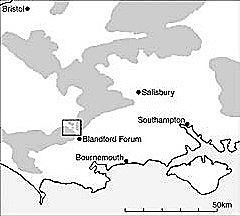
\includegraphics[width=0.7\textwidth]{figures/hambledon-location}
\end{center}
  \caption{Location of Hambledon Hill, from \citep[2]{Mercer:2008fk}}
  \label{fig:location}
\end{figure}

Hambledon Hill is a site of intense prehistoric activity, including two causewayed enclosures, two long barrows, neolithic defensive earthworks, \citep[xiii]{Mercer:2008fk} potentially as many as six round barrows \citep[12]{Mercer:2008fk} a hillfort and field systems. The site is situated in Dorset, South West England on the southern edge of Cranborne Chase. Between 1974 and 1986 Roger Mercer directed a programme of excavation the result of which is the published volume, \citet{Mercer:2008fk}. This was made up of nine seasons of large scale excavations, followed by more targeted investigations in the Everley Water Meadows in 1983 and 1984 and the hillfort in 1986 \citep[11]{Mercer:2008fk}. Figure~\ref{fig:excavations} shows the site, its key features and the main excavated areas. The interpretations offered are detailed and cover a broad range of topics, from a temporal perspective, they cover how the site developed over time, reproduced in figure~\ref{fig:hambledon-devel}. The interpretations of \citep{Whittle:2011kl} are more than just a linear progression of the site's features, they also offer probable lengths of time that each phase would have taken and duration of the gaps between phases. This interpretation is punctuated by key chronological events, such as the burial of individuals and the conflict surrounding the burning of the Stepleton Outwork. In addition it places the infilling and associated abandonment of areas of the site in their chronological context, showing how the focus of activity (or activities) shifted around the site over time. 

\begin{figure}
\begin{center}
	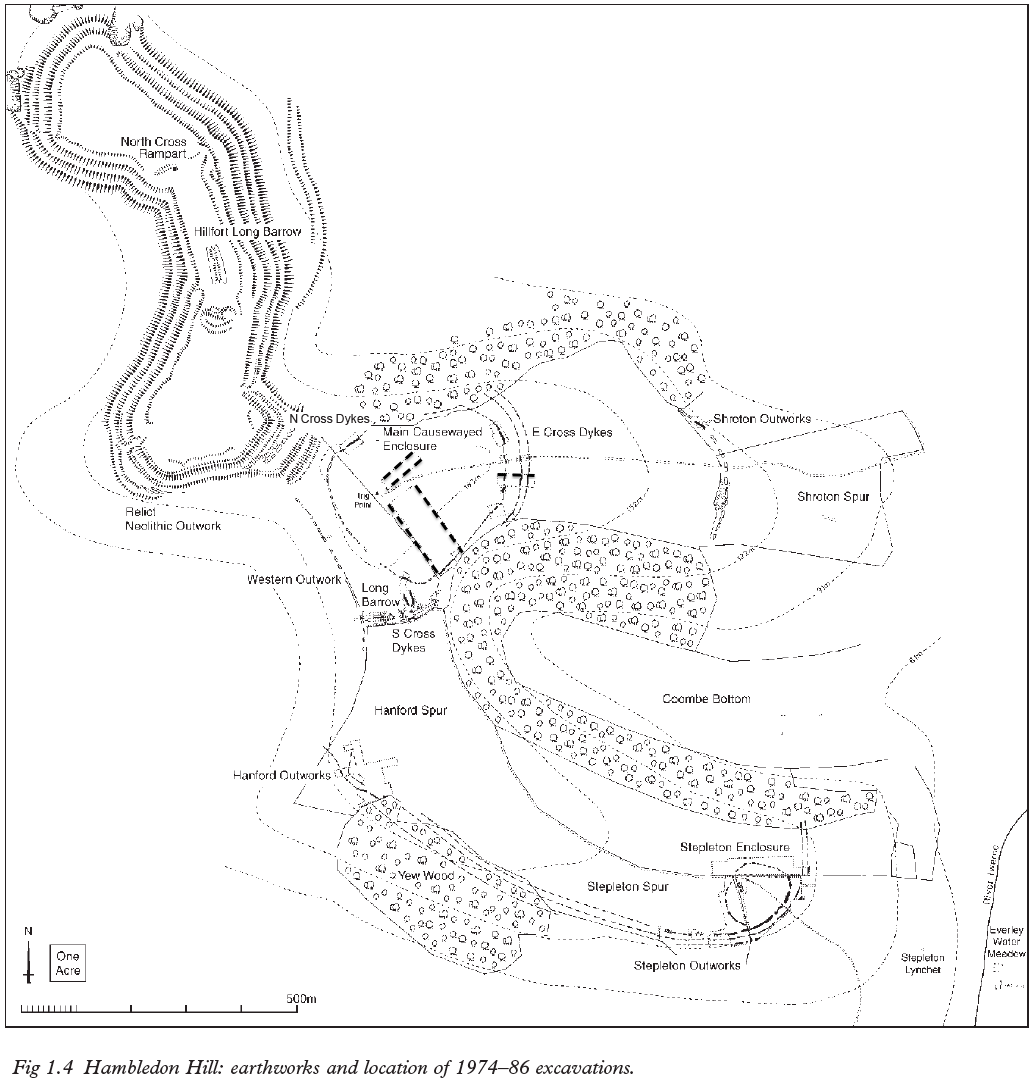
\includegraphics[width=0.9\textwidth]{figures/excavation-plan}
\end{center}
  \caption{Plan of main earthworks and locations on Hambledon Hill, from \citep[5]{Mercer:2008fk}}
  \label{fig:excavations}
\end{figure}

\section{The Temporal Evidence}

\begin{figure}
\begin{center}
	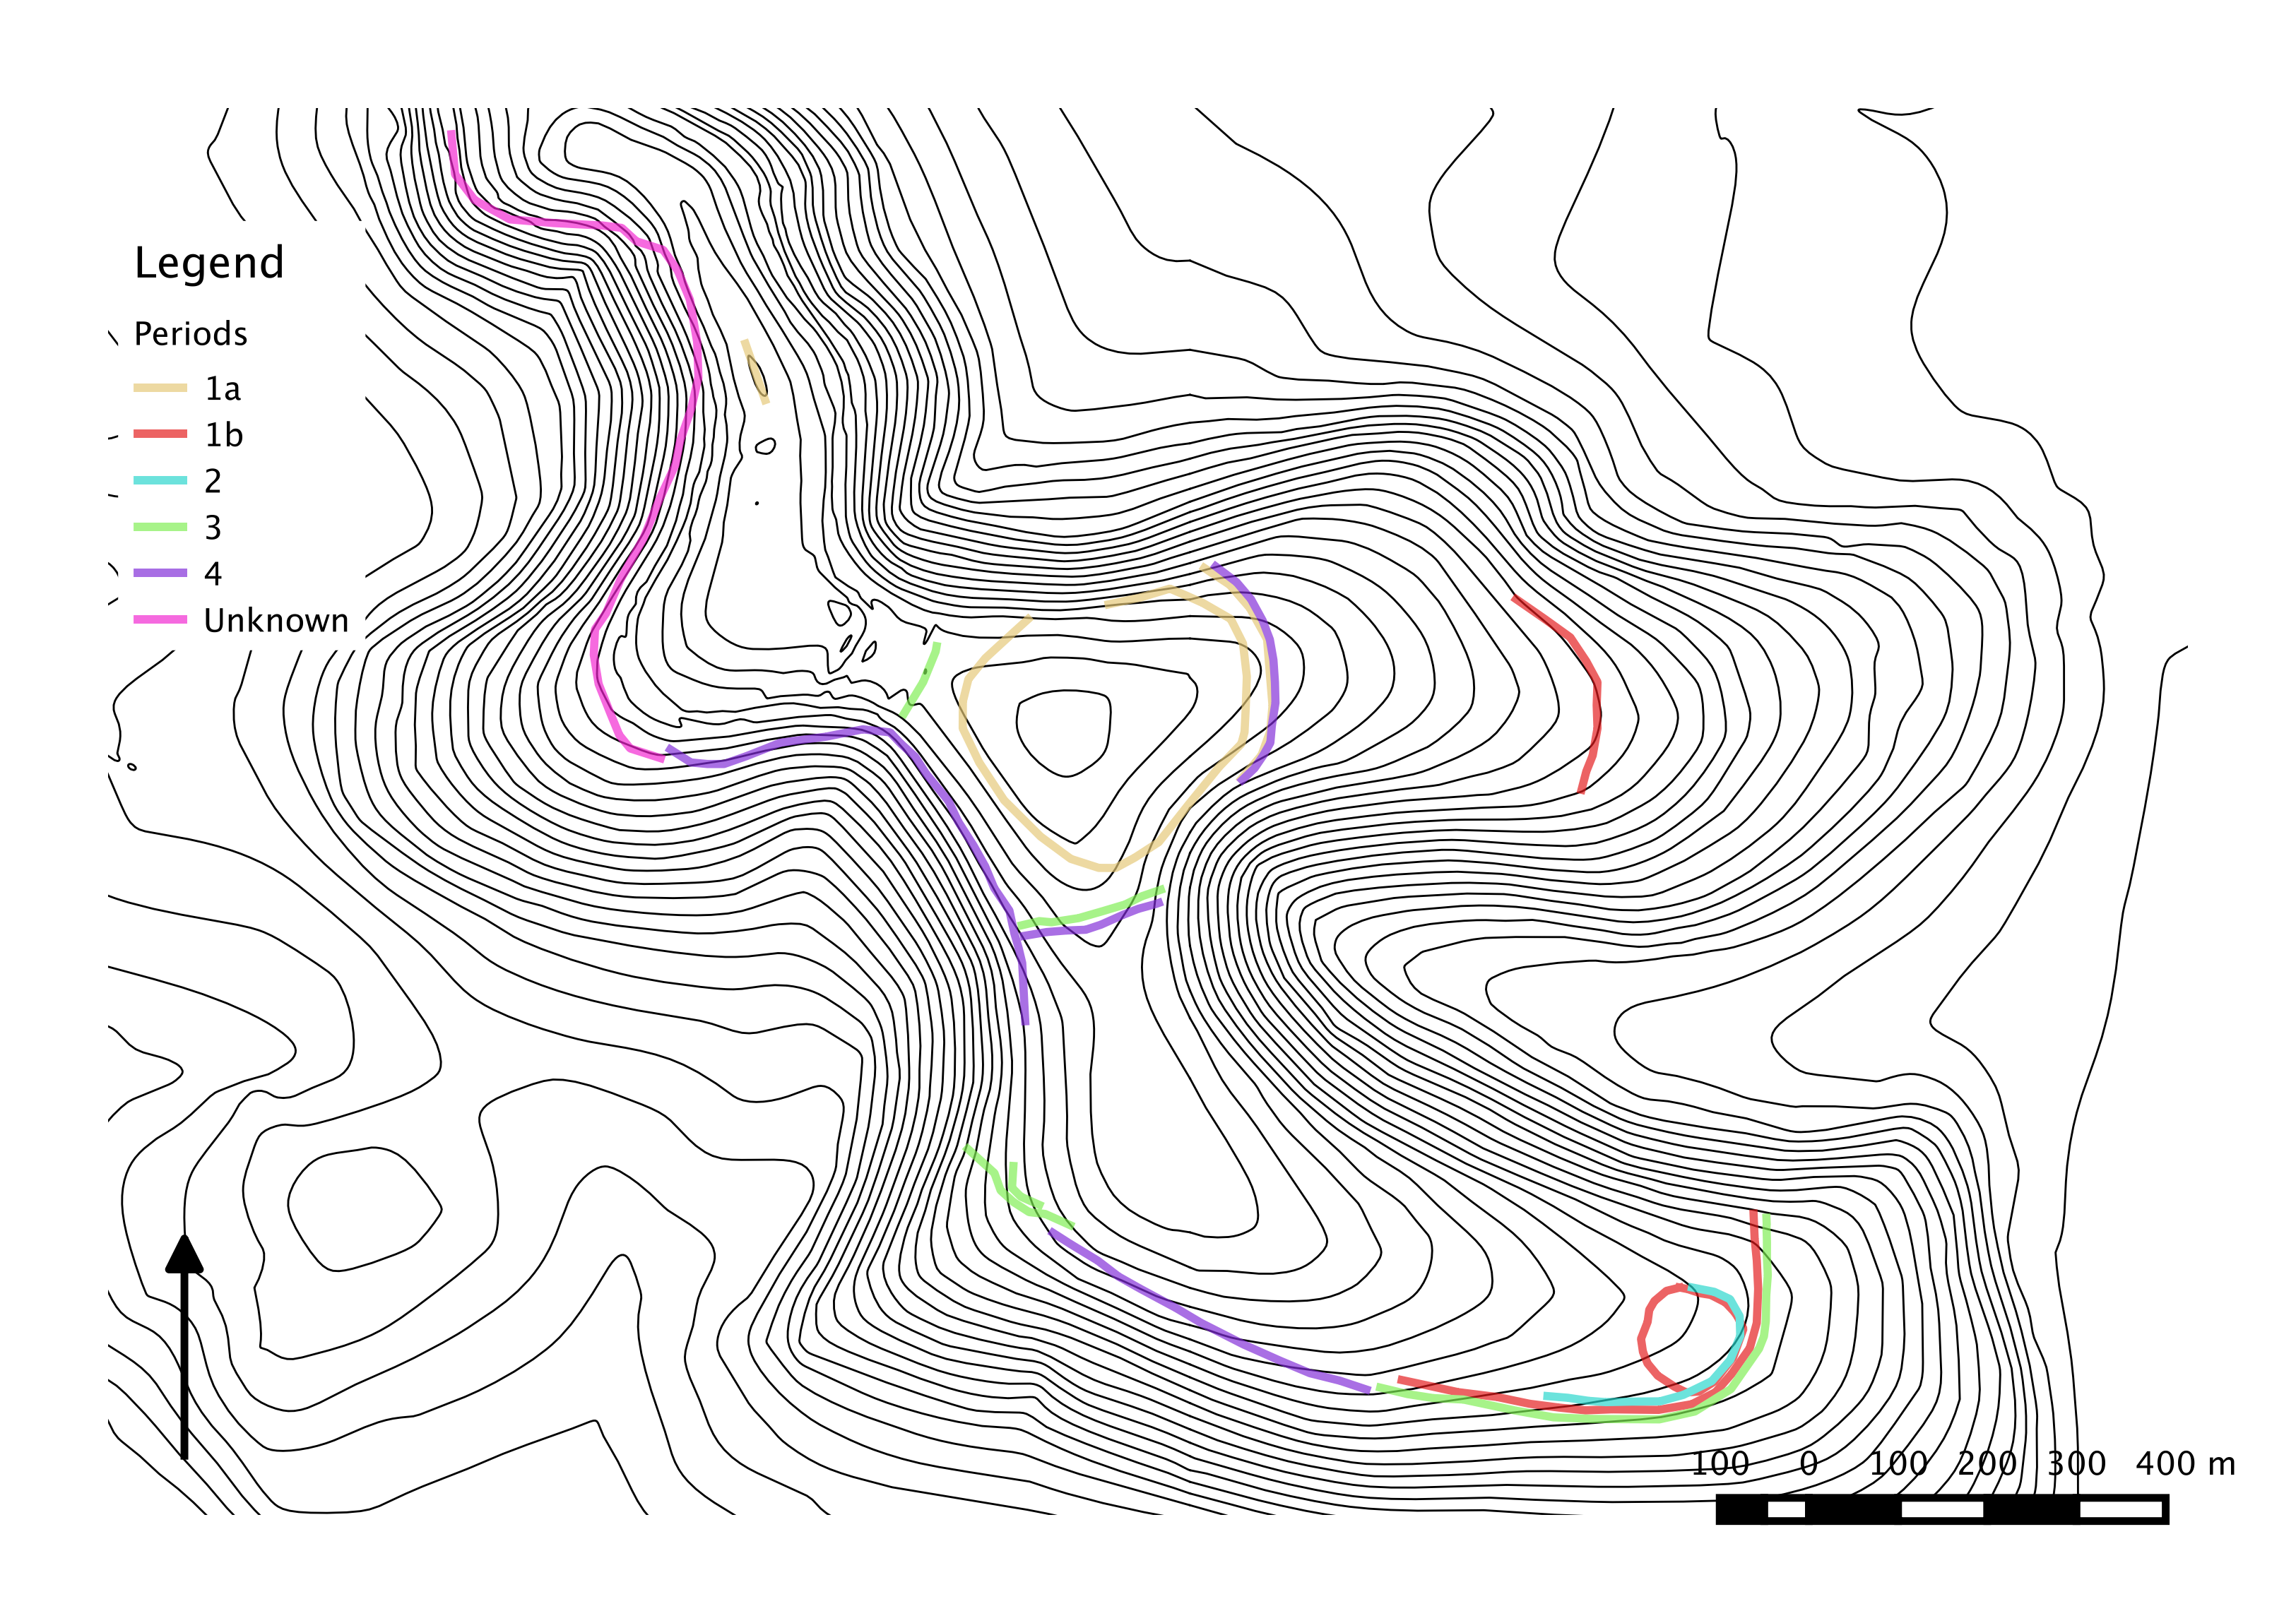
\includegraphics[width=0.9\textwidth]{figures/periods}
\end{center}
  \caption{Development of the Hambledon Complex by period, after \cite{Mercer:2008fk}}
  \label{fig:periods}
\end{figure}

The primary temporal evidence for Hambledon Hill comes from the the bayesian analysis documented in \citet{Whittle:2011kl}. This builds upon the original bayesian analysis, which formed a part of the report by \citet{Mercer:2008fk}. These analysis resulted in the definition of a sequence of discrete chronological periods of the site's Neolithic development, see figure~\ref{fig:periods}. The bayesian analysis was conducted using a subset of the radiocarbon dates combined with a model of the sites chronology, based on excavation evidence. 

\subsection{Pre-Neolithic Evidence}
The unequivocal temporal evidence for use of the site prior to the Neolithic comes from two areas, WOWK3 F4 and HN82 F279, plotted on figure~\ref{fig:meso1}. The feature WOWK F4 is interpreted as a likely Boreal age post in the original publication \citep[46]{Mercer:2008fk} on the basis of the compactness of the sample, and the lack of other charcoal samples of contemporary age from the surrounding area. This reduces the likelihood that it came from an episode of wider Boreal vegetation burning and subsequent redeposition. It is dated by one radiocarbon measurement (OxA-7816) to 8160-7590 cal B.C. \citep[43]{Mercer:2008fk}. 

\begin{figure}
\begin{center}
	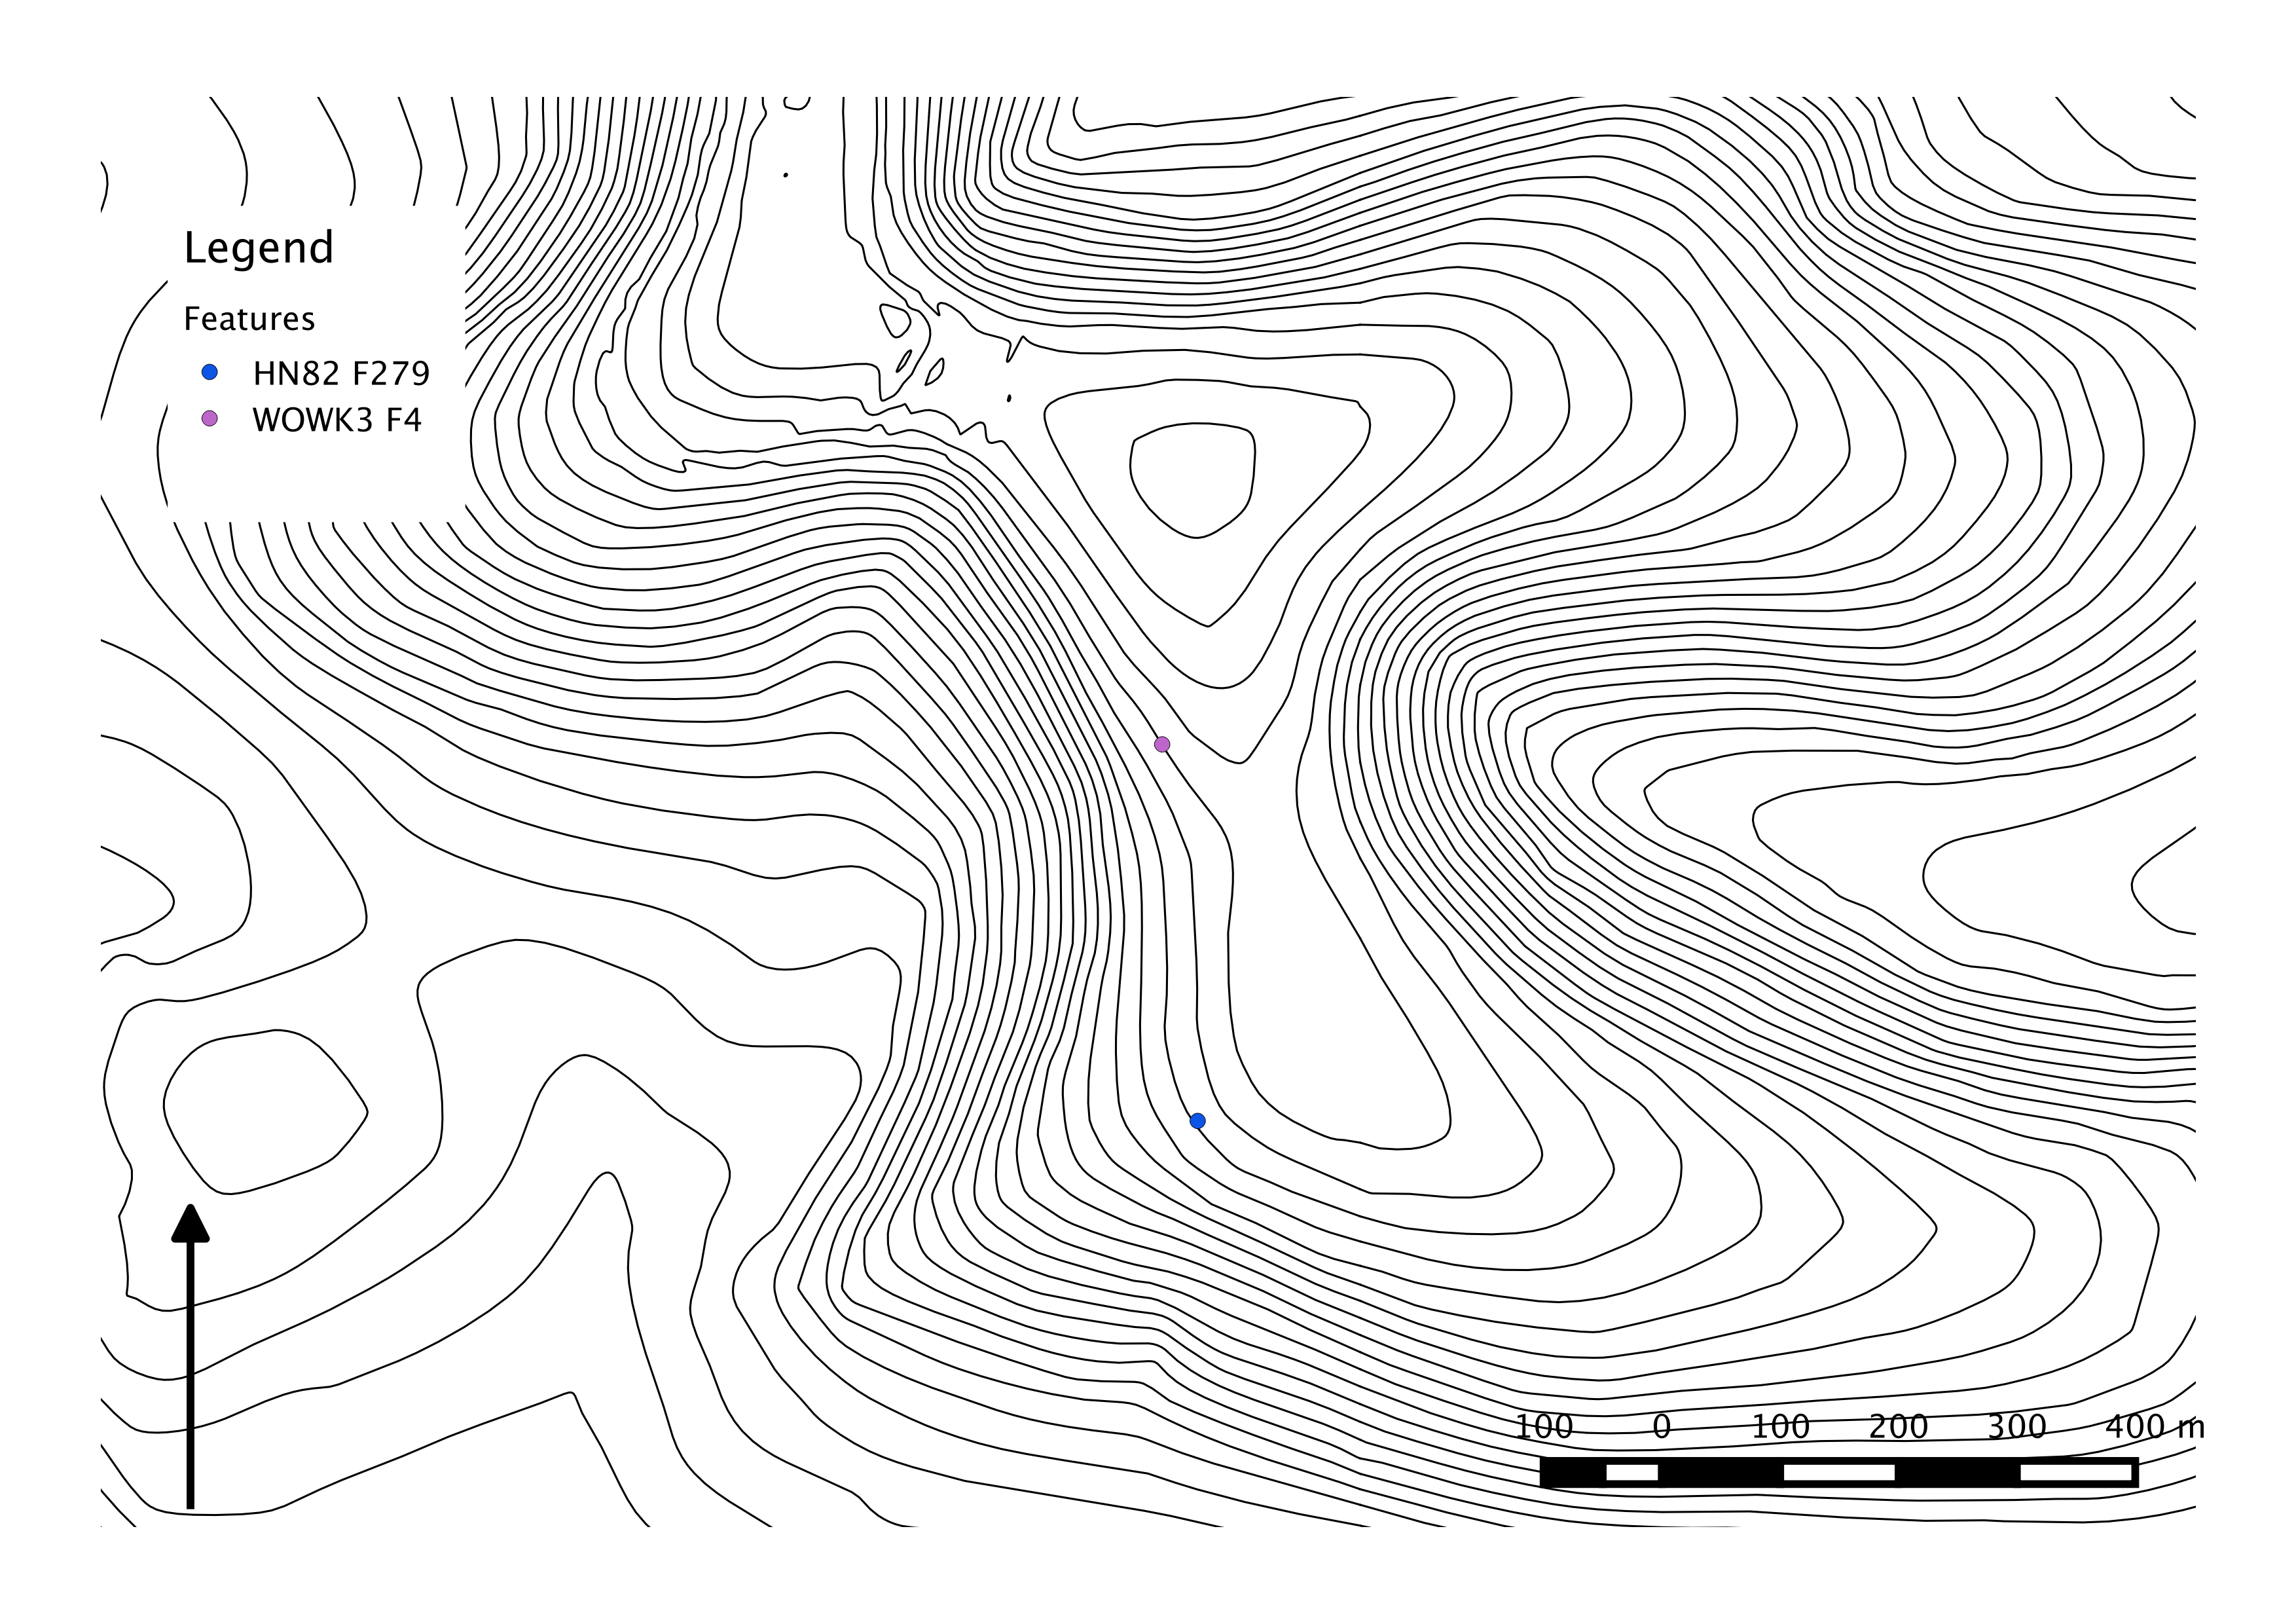
\includegraphics[width=0.9\textwidth]{figures/meso-features}
\end{center}
  \caption{Location of features containing Mesolithic dated samples}
  \label{fig:meso1}
\end{figure}

Feature HN82 F279 is much larger than the other, and is compared in the original report to the large pine posts, of a similar date, which stood near Stonehenge \citep[48]{Mercer:2008fk}. It was dated by two radiocarbon measurements (OxA-7845 and OxA-7846) giving dates of 7580-7200 cal B.C. and 7600-7380 cal B.C. \citep[46]{Mercer:2008fk}. The report also mentions feature F773 (undated) as being similar in form to F279 and the authors suggest the two are comparable \citep[46]{Mercer:2008fk}. There is also a third feature, F507, although the authors are less convinced by its comparability, suggesting it may instead be a part of the Neolithic bank structure. They are both from the same trench as F279.

Finally on the Stepleton spur, feature 4C F500 is identified by the authors as of a similar form to the features mentioned above, \citep[48]{Mercer:2008fk} but it has not been dated. 

Clearly there is evidence for activity on Hambledon Hill preceding its Neolithic use, although this evidence is relatively thin by comparison to later periods. The limited evidence available is focused on the West and South-West of the Hill, however feature 42 F500, if it were of a similar date, would show activity also took place on the opposite side.

\subsection{Pre-Neolithic and Neolithic Activity in the wider landscape}
There is also evidence of activity in the vicinity of Hambledon pre-dating and coinciding with its Neolithic use, the dating evidence is covered in \citep[151]{Whittle:2011kl}. This evidence comes from the Dorset Cursus, the Firtree Field Shaft, Thickthorn Down Barrow, Wor Barrow and the Monkton-up-Wimborne complex. The first three of these sites, along with the Hambledon features are shown on figure~\ref{fig:meso2}.

\begin{figure}
\centering
	\includegraphics[width=0.9\textwidth]{figures/meso-area}
  \caption{Location of pre-Hambledon Neolithic sites in the locality}
  \label{fig:meso2}
\end{figure}

This activity is mostly much more recent than the Boreal activity on Hambledon itself and overlaps the start of the main Neolithic use of the site. The evidence is clearly limited, for example the dating of Thickthorn Down is based on one radiocarbon sample, which may have been contaminated \citep[155]{Whittle:2011kl}. There is more evidence from the Dorset Cursus and Fir Tree Field shaft, however both of these were clearly in use for a long period of time. Any regularity, or evidence for continuous use is unclear from the models and radiocarbon dates. The case of the Cursus may not be helped by the potential for activities that attempted to keep it clean or clear. 

Crucially the Fir Tree Field shaft contains the earliest evidence for Neolithic activity in the area, a hearth associated with Neolithic Bowl pottery, dated to 3960-3755 cal BC (89\% probability, OxA-8009) or 3745-3710 cal BC (6\%) and probably to 3945-3850 cal BC (46\%) or 3845-3830 cal BC (5\%) or 3825-3785 cal BC (17\%) \citep[155]{Whittle:2011kl}.

\subsection{The Neolithic Complex}

\begin{figure}
\centering
	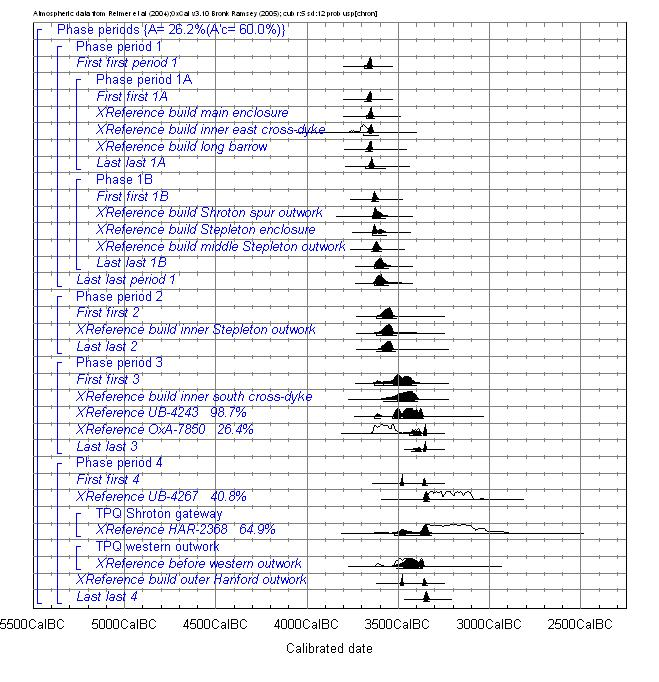
\includegraphics[width=0.9\textwidth]{figures/period-model}
  \caption{Posterior density estimates for the construction of the Neolithic earthworks and for the periodisation of the complex. Figure 4.14 from \citep[151]{Whittle:2011kl}}
  \label{fig:period-model}
\end{figure}

The results from the bayesian modelling were used to create a series of phases, reproduced as  figure~\ref{fig:period-model}, these are the same periods shown in figure~\ref{fig:periods}. This plan shows how the series of earthworks was built up across five discrete periods, although it does not show later re-use or re-cutting of earlier features. The original model is split based on geographic location in the original volumes, so that is how it shall be considered here.  

These bayesian models include a subset of the radiocarbon dates for the site, used to build a formal chronological model. However they lack any spatial reference. Using these models, plus the context information for each sample, it is possible to plot the rough location for each dated sample, shown in figure~\ref{fig:dates}. What this shows is concentrations of dates in certain parts of this site, clearly these are the excavated areas, however large sections of earthwork, which have been presented as part of the dated periods, have no associated dating evidence whatsoever. 

\begin{figure}
\centering
	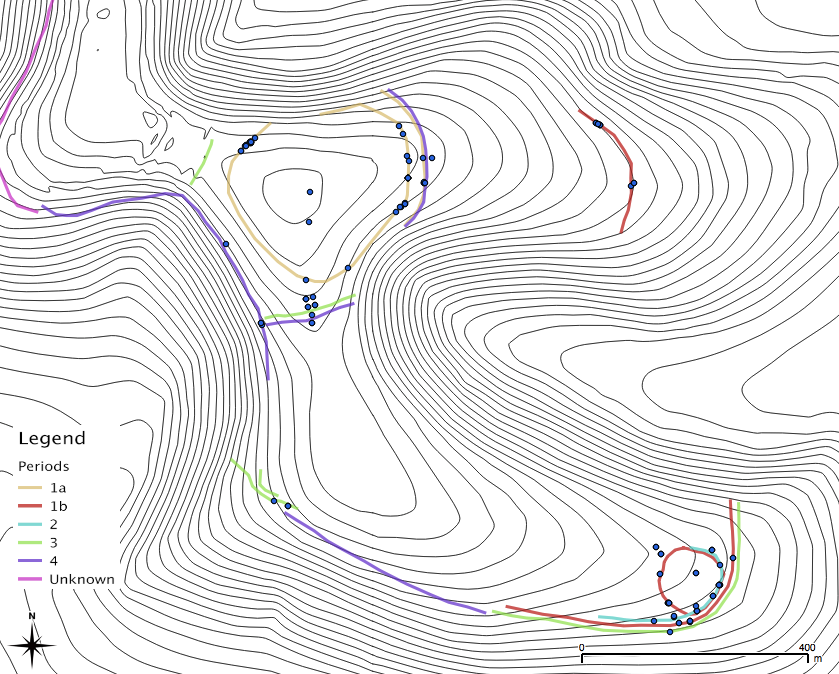
\includegraphics[width=0.9\textwidth]{figures/dates}
  \caption{Plot of the locations of all samples included in the bayesian model for the site, and key earthworks, for reference.}
  \label{fig:dates}
\end{figure}

\begin{figure}
\centering
	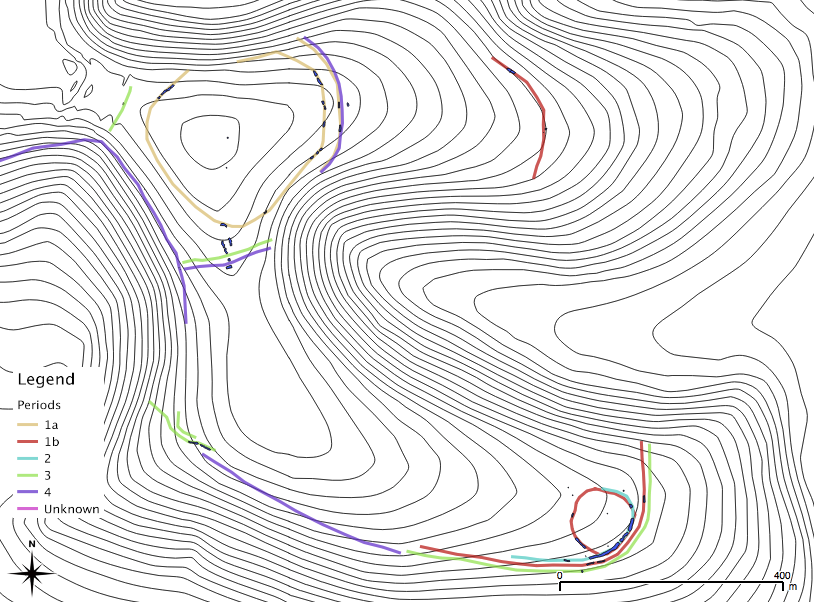
\includegraphics[width=0.9\textwidth]{figures/dated-features}
  \caption{Plot of all features dated via the bayesian model, and key earthworks, for reference.}
  \label{fig:dated-features}
\end{figure}

This in itself is not the spatial basis for discussion, instead the contextual information for each radiocarbon sample also specifies which ditch segment (or pit) it came from. These have been chosen as estimate find spots as the date locations are often only down to the segment and a point on a map therefore carries a misleading accuracy. Also assuming the date is a valid proxy for activity in the segment, such as its construction, or some form of use, and is not residual or incursive, then we can attribute that date to the feature, or an event involving it. Even more useful is when there are several dated samples, which have been included in the model, in this case we might have dates for multiple events involving the segment, and therefore a clearer idea of when that feature was in use. Rather than considering such dates independently, it makes sense to combine them spatially, as they all relate to the same segment, and are therefore not independent observations. Figure~\ref{fig:dated-features} shows for the whole site those features which have been dated via the bayesian model, overlain on the earthworks, by period. 

\subsubsection{The Central Area}
The central area of Hambledon Hill covers the causewayed enclosure, built during phase 1a. The dating evidence for this is modelled in two diagrams in \cite{Whittle:2011kl}. Figure~\ref{fig:central1} and figure~\ref{fig:central2} shows these two diagrams along with plans of the features dated by each model.

\begin{figure}
\centering
	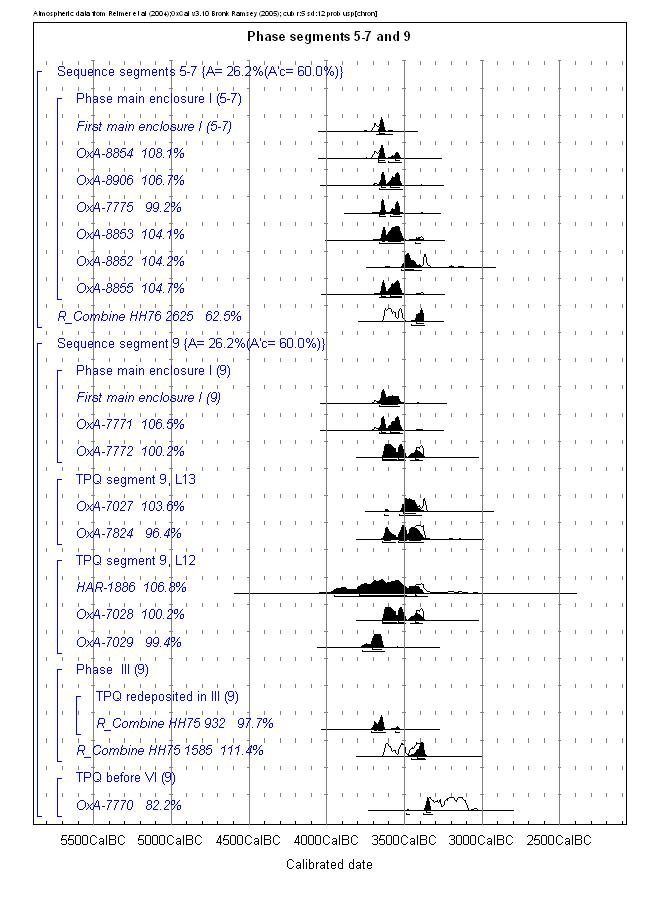
\includegraphics[width=0.7\textwidth]{figures/model1}
	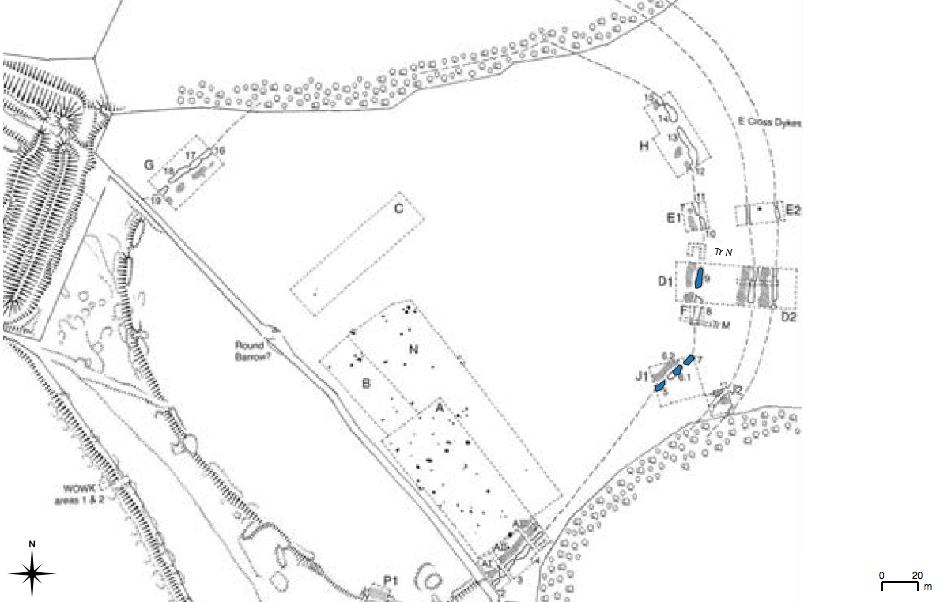
\includegraphics[width=0.9\textwidth]{figures/model1-plan}
  \caption{Bayesian model for the central area and plan of the features dated, from fig 4.8 \citep[139]{Whittle:2011kl}}
  \label{fig:central1}
\end{figure}

What becomes immediately clear, is that within the excavated areas, there is good coverage of the bayesian model on ditch segments for the central causewayed enclosure. Figure~\ref{fig:central1} is more localised in the South-East, where as figure~\ref{fig:central2} covers the remaining excavated areas. Having said that, figure~\ref{fig:central1} only covers four ditch segments, and figure~\ref{fig:central2} covers ten, combined they perhaps date around one third of the ditch for the causewayed enclosure on Hambledon Hill. 

\begin{figure}
\centering
	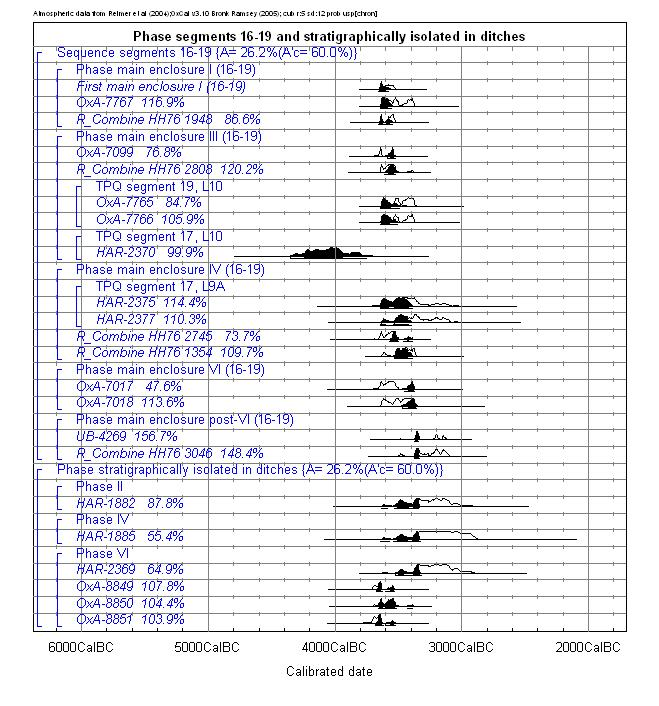
\includegraphics[width=0.7\textwidth]{figures/model2}
	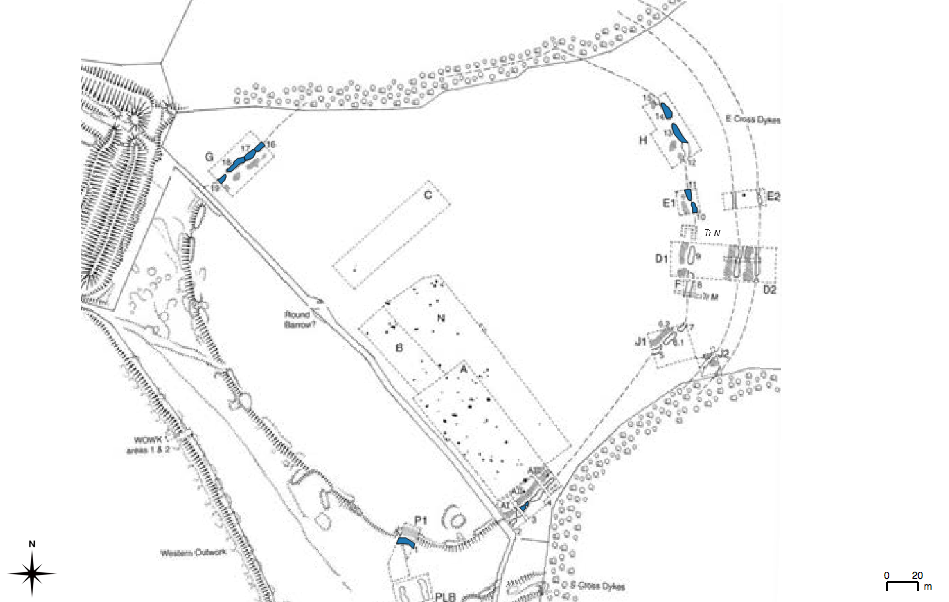
\includegraphics[width=0.9\textwidth]{figures/model2-plan}
  \caption{Bayesian model for the central area and plan of the features dated, from fig 4.9 \citep[140]{Whittle:2011kl}}
  \label{fig:central2}
\end{figure}

However several of the ditch segments dated in figure~\ref{fig:central2} are included under the model as ``stratigraphically isolated in ditches''. These are included primarily as additional dates for phases where dated evidence is scarce, providing a comparison to make sure other dates are not residual or incursive. The approximate locations of those dates included in the stratigraphically isolated section is shown in figure~\ref{fig:central-isolated}. When these are excluded the dating evidence from the primary fills of the causewayed enclosures comes from two sections of ditch segments, segments five to seven, nine and 16-19. All of the dates from these two sections of ditch segment are included in table~\ref{tab:central-dates} along with details about which segment they came from, and phase.

\begin{figure}
\begin{center}
	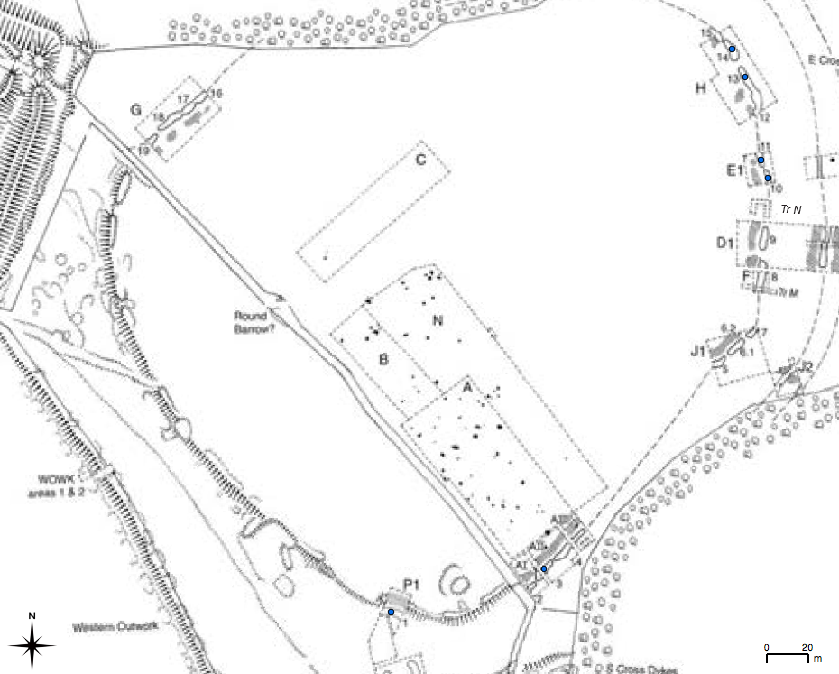
\includegraphics[width=0.9\textwidth]{figures/central-isolated.png}
\end{center}
  \caption{Plot of all locations of dates identified as stratigraphically isolated in fig 4.9 \citep[140]{Whittle:2011kl}}
  \label{fig:central-isolated}
\end{figure}

\csvautolongtable[
  table head= \caption{List of all dates included in the bayesian model of the central area, the calibrated date is at the 95\% confidence interval}\label{tab:central-dates} \\\hline
               \csvlinetotablerow\\\hline
               \endfirsthead\hline
               \csvlinetotablerow\\\hline
               \endhead\hline
               \endfoot,
]{figures/central-dates.csv}

There are six dates for the first phase (phase I in the original report) from segments five to seven, grouped as ``Phase main enclosure I'' \citep[139]{Whittle:2011kl} of these OxA-8852 stands out as it is not statistically significant with the rest, and is in fact significantly younger \citep[398]{Mercer:2008fk}. OxA-8852 is one of two dates from segment 6.2, the other is assumed to be redeposited on the basis that it is younger, despite being consistent with the dates from other segments. For these segments the only other dated event is the end of Phase II, which is dated by a sample from segment 6.2. The next segment, segment nine, while included with five to seven in the original model, and discussion, is in fact from a distinct area of the excavation. In this segment phase I is dated by two samples, phase II is dated by charcoal samples, which are treated as a terminus post quem. Phase III contains samples consistent with the underlying layers and but also potentially redeposited samples. Segments 16-19, are on the opposite side of the circuit to five to seven, here phase I and II are dated by samples from a child burial cut into the base of segment 18, and also bone fragments from segment 16. Phase III is dated by a terminus post quem from segment 17, and one also from segment 19. Phase IV and phase VI are dated by samples from segment 17. Across these areas, there are 11 dates from phase I, five from phase II, two from phase II / phase III interface, ten from phase III, six from phase IV, three from phase VI and three post phase VI. Clearly phases I to III make up the bulk, at 18 samples, where as phases IV and beyond are only dated by 12 samples. When considered from a purely temporal perspective this looks to be a good set of dates, however this is only looking at the data from a one dimensional perspective. When the spatial dimension is included, it becomes clear that the distribution is far from even. The phase I and II samples are mostly from the areas of segment five to seven and nine, and phase III samples are split between segments nine, 17 and 19. And phase IV, IV and post-IV are almost exclusively from segment 17.

The original report found that the enclosure was likely built in a short span of time, although not necessarily at the same time, based on the consistent results provided by the 11 samples (if OxA-8852 is excluded) and the nature of the samples, coming mostly from articulated or articulating deposits \citep[401]{Mercer:2008fk}. But when we look at those areas on a plan, we can see that the earliest evidence for the causewayed enclosure comes from a small group of segments on one side of the circuit, and one segment on the opposite side. The original report used this as evidence that the whole circuit was built in a relatively short period of time. This is one interpretation, it could also be that the two areas dated were constructed at the same time, but not necessarily the entire circuit. If we include the spatial evidence that these two areas were almost exactly opposite this could be interpreted as evidence that opposite sides of the circuit were worked on at a similar time. While the evidence does support the original conclusions about the construction of the enclosure, it is open to alternative interpretations, the limited nature of the evidence, in particular its spatial spread is a constraint on our knowledge about the construction of the ditch circuit. By considering the spatial pattern the original conclusions are less secure than they initially appeared. 

\subsubsection{Cross Dykes and the Long Barrow}
This model shown in figure~\ref{fig:crossdykes} is a bit of a ``catch all'' for those parts of the site that do not fit into the other main areas, instead forming a periphery to the central area.

\begin{figure}
\centering
	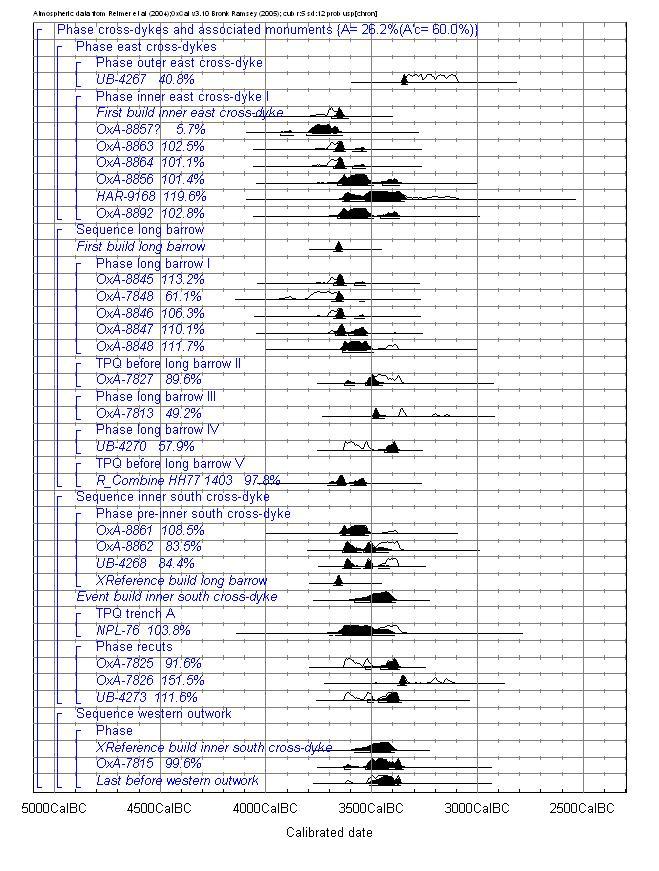
\includegraphics[width=0.7\textwidth]{figures/model3}
	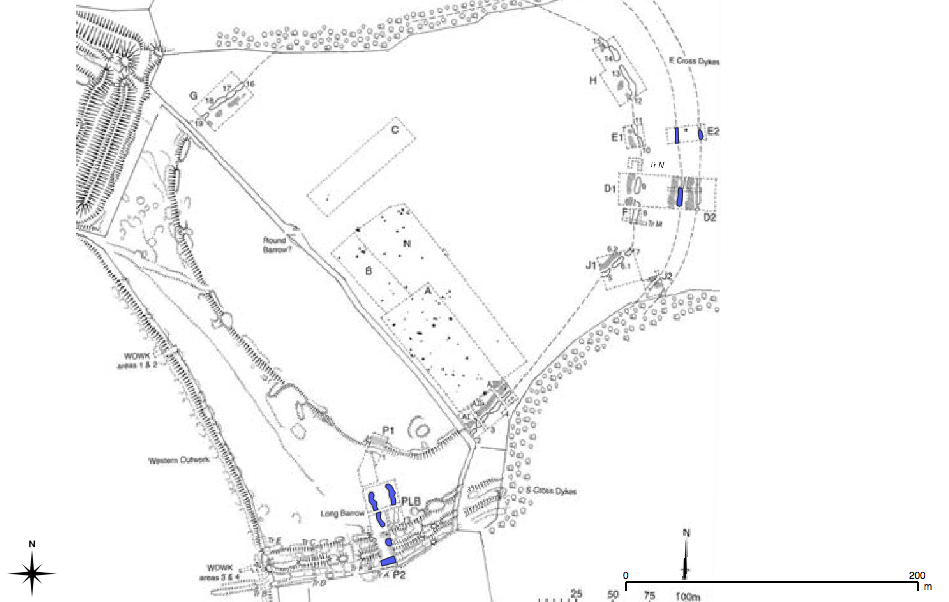
\includegraphics[width=0.9\textwidth]{figures/model3-plan}
  \caption{Bayesian model for the cross dykes, etc and plan of the features dated, from fig 4.10 \citep[139]{Whittle:2011kl}}
  \label{fig:crossdykes}
\end{figure}

Firstly, the east cross-dykes, the outer east cross-dyke only gave one date, UB-4267, which calibrated to 3360-2700 cal B.C. (95\% confidence) \citep[122]{Whittle:2011kl}. This is considerable later than the dates for the inner east cross-dyke and for most of the rest of the central area. It is possible that the dated material is in fact from an extension of the original segment \citep[401]{Mercer:2008fk} and as the date is closer to those of recuts of the south cross-dyke it could represent a phase of broader re-furbishment of the site. However, with only one date to go on, this is purely speculative, and when examined on a plan of the site, the two areas are quite far apart, making some coincidental localised recutting and extending an equally likely proposition. 
 
The inner east cross-dyke, having five dates included in the model provides a bit more to go on, however four were from the same segment, segment four. Of these, three were taken from charcoal and one was a bulk sample (HAR-9168). OxA-8856 came from a red deer antler tip, and OxA-8892, in segment five, a cattle radius fragment. \citet[401]{Mercer:2008fk} note that all of these measurements are statistically significantly different. \citet[136]{Whittle:2011kl} state that the cross-dykes were built at the same time as the main enclosure. Based on the limited evidence available this does not seem particularly contentious, but the evidence for the east cross-dykes is very limited spatially, and also temporally, as all the samples are from phase I.
 
The south long barrow was extensively excavated, as shown in figure~\ref{fig:crossdykes} and the dates for it come from three quadrants. In total it produced ten dates that were included in the model, of which half came from phase I, two came from a TPQ before phase V and the rest were one per phase for II, III and IV \cite[401]{Mercer:2008fk}. These last three all came from quadrant LB3, where as the five for phase I came mostly from LB2, with one coming from LB4. While it seems highly likely that a monument such as this would have been constructed in one go, it would have been preferable to have a continuous chronology from a single area. Especially as all these dates came from the ditches, so it is possible that the dates for later phases may be activity in a specific quadrant or side of the long barrow.

Next on the model is the inner south cross-dyke, sealed beneath the cross-dyke were several samples pre-dating the bank construction, one UB-4268, a cattle tibia fragment. OxA-8861 and OxA-8862 are from a possible post hole, treated as a terminus post quem \citep[402]{Mercer:2008fk}. These samples are not included in figure~\ref{fig:crossdykes} as it was not possible to determine their spatial location from the information included in \cite{Whittle:2011kl} and the plans in \cite{Mercer:2008fk} are not reproduced at a high enough quality to identify the feature in WOWK area three. The features dated by other samples in the model are only rough approximations, as the plan in \cite{Mercer:2008fk} is a low quality reproduction, and is quite confused in this area of the site. Only one of the samples is from phase I, but it is a bulk sample containing oak charcoal and so has a broad posterior, it is only usable as a terminus post quem. The other samples are later, from phase VI. Clearly, a spatio-temporal assessment of the inner south cross-dyke is problematic as it is very difficult to determine the positions of the features dated. What we can determine is that the possible post hole, which may pre-date the bank, or be part of its structure \citep[402]{Mercer:2008fk} is at the western-most end of the cross-dyke, whereas the datable material is from its center.

Finally in this model is the western outwork. This is also not included in the plan in figure~\ref{fig:crossdykes} as, while the location of WOWK area two is marked, the features excavated are not. Without a clearer plan, or more information it would only be possible to locate this date to the excavated area. In summary, these features on the periphery of the central area are, apart perhaps from the long barrow, generally lacking in dating evidence, especially in terms of  spatial spread. 

\subsubsection{Stepleton Enclosure and Outworks}

\begin{figure}
\centering
	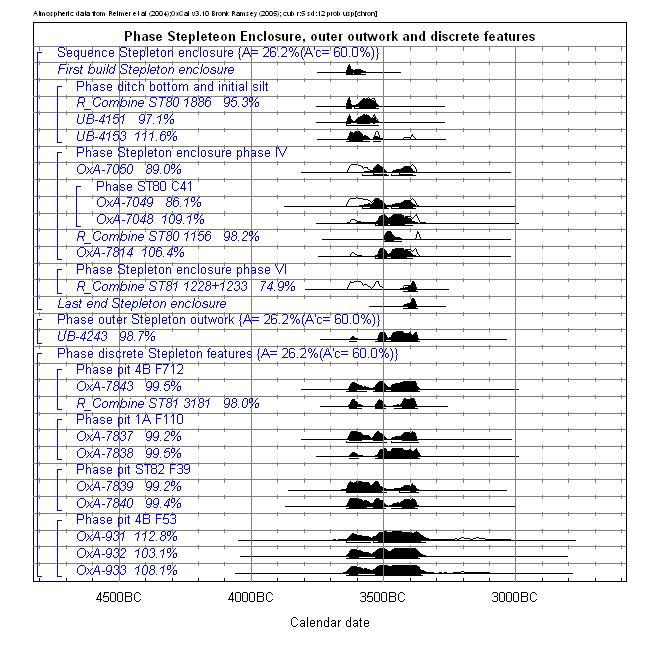
\includegraphics[width=0.7\textwidth]{figures/model4}
	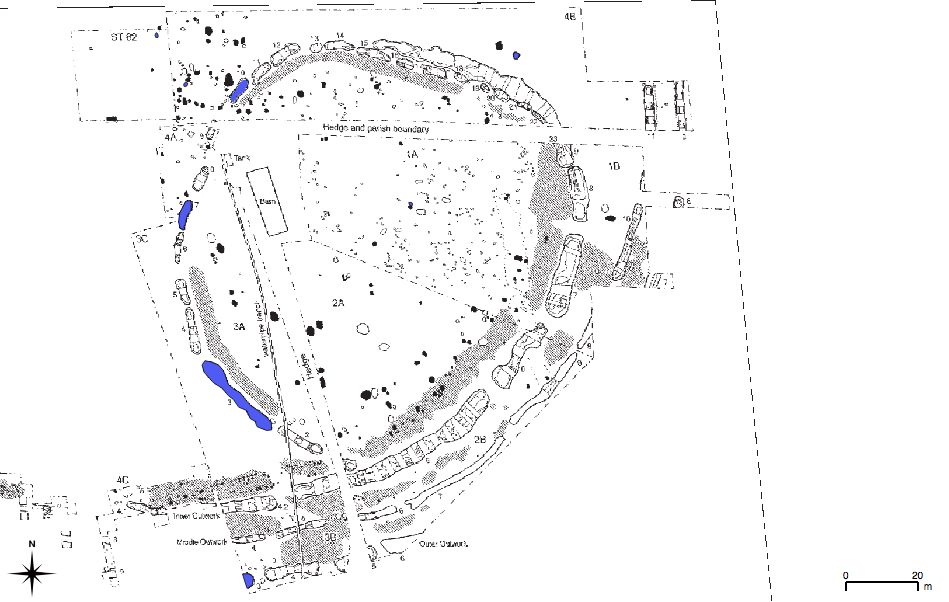
\includegraphics[width=0.9\textwidth]{figures/model4-plan}
  \caption{Bayesian model for the Stepleton enclosure and plan of the features dated, from fig 4.11 \citep[142]{Whittle:2011kl}}
  \label{fig:stepleton}
\end{figure}

The Stepleton enclosure is a causewayed enclosure with a series of outworks, to the south-east of the main enclosure. Figure~\ref{fig:stepleton} shows the bayesian model for this area, from fig 4.11 \citep[142]{Whittle:2011kl} and a plan of the excavation, with the ditch segments and pits that have contributed dates to the model highlighted in blue. The plan shows that the dates for the enclosure come from three ditch segments and four pits, of which one is inside the enclosure and the other three are outside. This model also provides a date for the outer outwork, with one segment being dated. 

The initial construction of the ditch is dated by five measurements on three antler implements, from the base of ditch segment three, these are assumed in the original report to be close in age to the ditch's excavation \citep[394]{Mercer:2008fk}. There are no dates included in the bayesian model for phase II or phase III which makes up most of the fill, phase IV is dated by short life charcoal from a pit cut into the fills, (OxA-7048, OxA-7049, OxA-7050) and samples from an articulated dog skeleton (UB-4138 and OxA-7041). Also included in the model for phase IV is a sample from segment ten, from an articulated upper body of a woman (OxA-7814). To complete the sequence, two dates were taken from segment seven, from samples of sooty residue on two sherds, however the original report notes that these two samples were statistically significantly different \citep[394]{Mercer:2008fk}. Clearly the main focus of this part of the model is on segment three, although we can see from the plan in figure~\ref{fig:stepleton} that this was a large segment and it is not clear whether all the dates were taken from samples found close together, or at opposite ends of the segment. The additional dates from segments seven and ten rely on the phases being comparable across the different segments, and dating the whole enclosure from this limited evidence relies on the phases being comparable across the whole enclosure. \citet[394]{Mercer:2008fk} note ``it is impossible to tell if the sequence in every segment is synchronous'' which is unfortunate, as this is clearly a requirement for combining dates from multiple segments into the same phases and for extrapolating the dates of these phases across the wider area.

Five discrete features within and around the Stepleton enclsoure were also dated, only four shall be considered here, as feature 1A F70 an articulated child burial (dated by OxA-7836) was accidentally missed out when the model was rebuilt for Gathering Time (Alex Bayliss, personal communication) and so does not feature in the model shown in figure~\ref{fig:stepleton}. The other internal feature 1A F110 contained a deposit of barley, dated by OxA-7837 and OxA-7838. 4B F712 was also a burial, to the north-east exterior of the enclosure, with two samples from the skeleton dated (OxA-7818 and UB-4311) and one from charred hazelnut shells (OxA-7843) \citep[396]{Mercer:2008fk}. The other two features were both to the north-west exteriors, one, ST82 F39 dated by a quantity of emmer wheat (OxA-7839 and OxA-7840) and the other 4B F53 a grape pip, and cereal grains (OxA-931, OxA-932 and OxA-933). Spatially, these features are all distinct, and they are treated as such in the bayesian model, being grouped under a phase keyword, implying no ordering to the dates. As there is no chronological ordering of these features, or of their place within the Stepleton enclosure the bayesian modelling processes has had little effect on their dates, as can be seen in figure~\ref{fig:stepleton}. The only useful output from including this is to confirm via the agreement index that this chronological modelling is correct.

The outer Stepleton outwork, dated by one sample (UB-4243) from an articulated skeleton found at the base of a segment terminus, which the original investigators assumed to have been placed soon after the ditch was cut \cite[396]{Mercer:2008fk}. As we can see from figure~\ref{fig:stepleton} the outer outwork is the least investigated, and this single date really provides little more than a time around which this part of the outwork was being built. As so little of the outer outwork has been investigated we can't attempt to suggest that its ditches were cut synchronously.

The middle and especially the inner outworks had a greater number of dated samples, and the model for these was split into a separate diagram from the rest of the earthworks on the Stepleton spur it is reproduced in figure~\ref{fig:stepleton2} along with a plan of the ditch segments that produced the dates.

\begin{figure}
\centering
	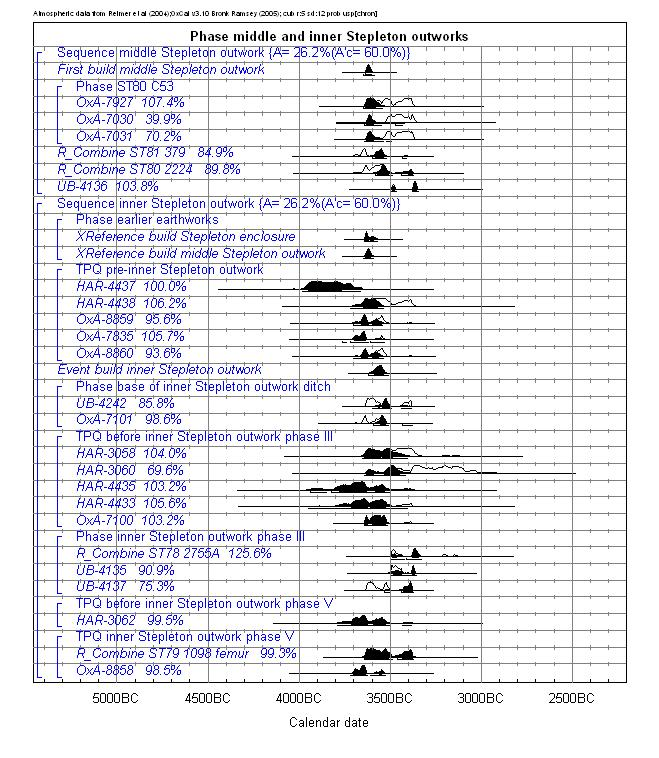
\includegraphics[width=0.7\textwidth]{figures/model5}
	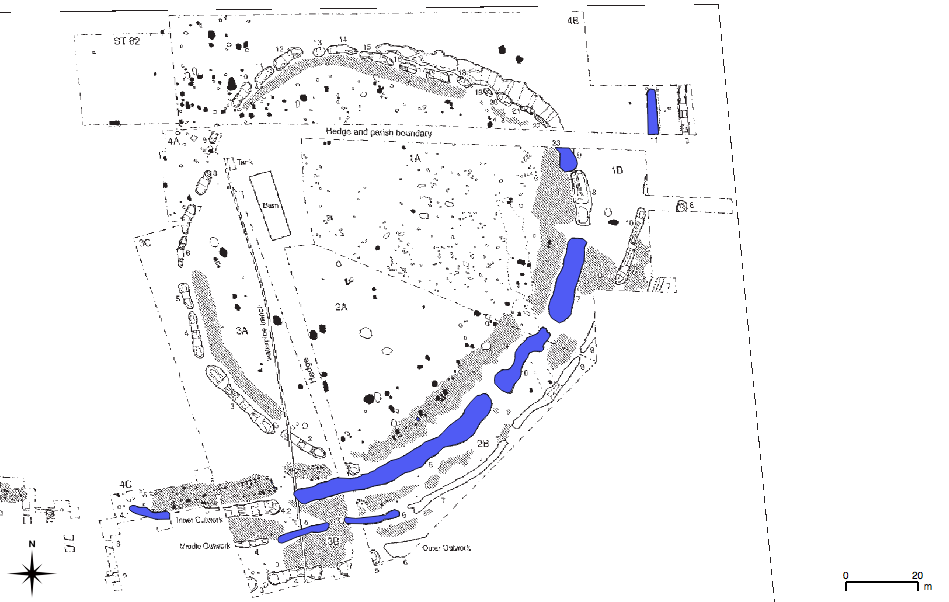
\includegraphics[width=0.9\textwidth]{figures/model5-plan}
  \caption{Bayesian model for the middle and inner Stepleton outworks and plan of the features dated, from fig 4.12 \citep[143]{Whittle:2011kl}}
  \label{fig:stepleton2}
\end{figure}

From phase I of the middle outwork come three dates on single fragments of short life charcoal taken from the base of segment six (OxA-7030, OxA-7031 and OxA-7927) that the original report concluded were homogenous and freshly deposited on the basis of a lack of significant statistical difference \cite[395]{Mercer:2008fk}. There were no phase II samples from segment six, but one from segment five (OxA-7024 and OxA-7025) and one from segment 11, (OxA-7035 and OxA-7036) both articulating. Phase III is dated by one sample from segment six (UB-4136) an articulating cattle vertebra from rubble fills \cite[395]{Mercer:2008fk}. In the original report, the authors mention that OxA-7030 has a low index of agreement at 41.8\% (but 40.4\% in the model from \citealp{Whittle:2011kl}) which they put down to an artefact of statistical scatter \cite[395]{Mercer:2008fk}. It could also be a by product of assuming that segments five, six and 11 are synchronous, as the dates from five and 11 above OxA-7030 could lead to a low agreement value if they were not strictly following OxA-7030. The approximate locations of all these dates are shown in figure~\ref{fig:pre-outwork}.

\begin{figure}
\begin{center}
	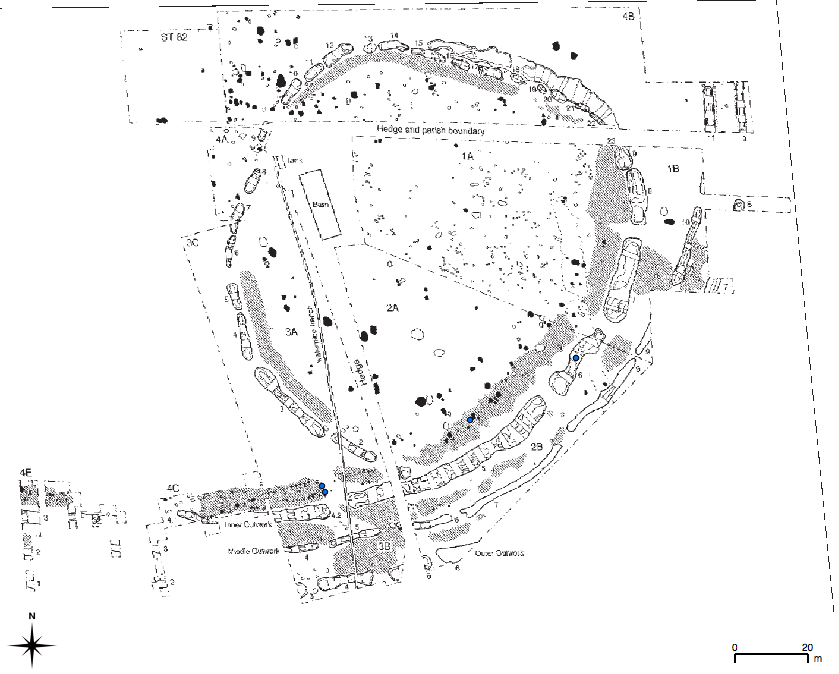
\includegraphics[width=0.9\textwidth]{figures/stepleton-preoutwork}
\end{center}
  \caption{Plot of locations of dates preceding the inner Stepleton outwork}
  \label{fig:pre-outwork}
\end{figure}

Turning to the inner outwork, the model shown in figure~\ref{fig:stepleton2} clearly shows that two sets of dates are included which pre-date the outworks construction. At the very bottom are references to other sections of the overall model, first the building of the middle outwork, and then the building of the Stepleton enclosure. The first relationship was based on the result of excavation evidence, and the second from air photographic evidence \cite[395]{Mercer:2008fk}. Following this is a set of five dates, HAR-4437 and HAR-4438 are from features situated on the enclosure side of segment 4.2, in a location at the end of the bank. These samples are from charcoal of posts burnt in-situ in the gateway \cite[395]{Mercer:2008fk}. The next date, OxA-7835 is from the bank behind segment five, this is from a sample of an articulated burial, which in the original report is assumed to have been buried under the bank \cite[395]{Mercer:2008fk}. And OxA-8859 and OxA-8860 two charcoal samples from the surface of the primary silt of segment six, which the original investigators assumed to be a part of the rampart breastwork \cite[395]{Mercer:2008fk}. This last date is considered to pre-date the construction of the outwork, as the building of the outwork followed the burning of the enclosure. As can be seen in figure~\ref{fig:pre-outwork} these dates stretch along only a part of the inner outwork, from segment six to segment 4.2. 

From phase I of the inner outwork, two dates are included in the model. UB-4242 from segment seven and OxA-7101 from segment nine. These were both from articulated burials laying on the ditch bottom  \cite[395]{Mercer:2008fk}. Following this in the model is a set of samples from various charcoal fragments, which are included as a terminus post quem as they may have derived from an earlier event \cite[395]{Mercer:2008fk}. HAR-3058 and HAR-3060 were from segment seven, HAR-4435 from segment four and HAR-4433 from segment five. Also included in this grouping of the model is OxA-7100 from segment seven, a sample from an adult skeleton, which may have been redeposited \cite[396]{Mercer:2008fk}. There were no samples from phase II, from phase III there are four samples from articulating remains in three segments, UB-4137 from segment six, UB-4135 from segment five, OxA-7044 and OxA-7045 from segment seven. These samples are statistically significantly different, in the original report this is put down to the rubble fills taking time to accumulate, based on the irregularity of the fill, and the varying locations in the fill that the different samples came from \cite[395]{Mercer:2008fk}. It could, of course, also be related to the samples coming from three different segments, lacking a homogeneity across all three in the formation of this fill. HAR-3062 from segment seven is then modelled singly as a terminus post quem, this is a charcoal sample, which as with the others may related to an earlier event. Finally, there are three samples from segment five, (OxA-7026, OxA-7059 and OxA-8858) coming from a dump of sheep remains, which the investigators believed to have been redeposited \cite[396]{Mercer:2008fk}. There is a sequence of six dates through segment seven, one from segment six, five from segment five, one from segment four and one from segment nine. However looking at figure~\ref{fig:stepleton2}, it is clear that segment five is particularly long, and the samples could have occurred anywhere along it's length. The other segments are fairly regular, with six and seven being about the same length, as are four and nine. The agreement measurement from the samples is used in the original report to suggest a common history of construction across the segments, \cite[396]{Mercer:2008fk} but there seems to be a certain circularity of argument around this, as the agreement values have been used to define the model. It would be more valuable if there was physical evidence of a common history of construction.

\subsubsection{Hanford Outworks, Shroton Spur Outworks and discrete central area features}

\begin{figure}
\centering
	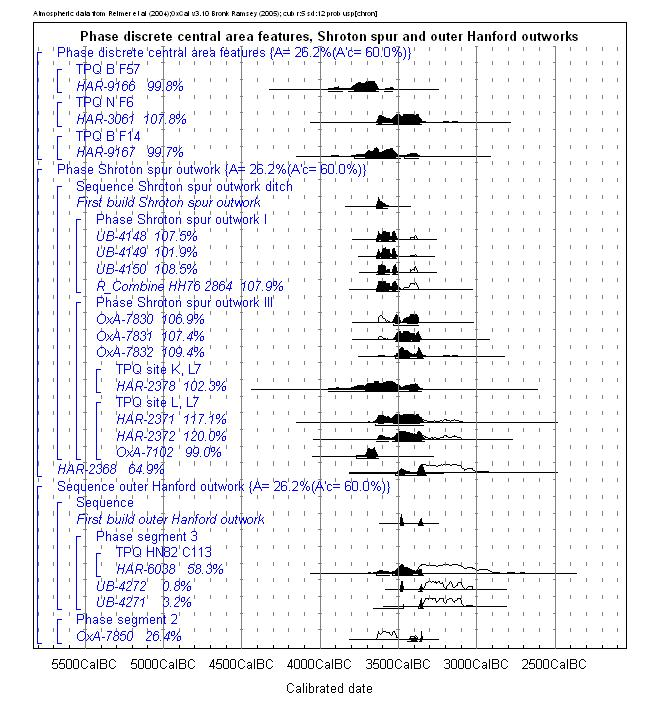
\includegraphics[width=0.7\textwidth]{figures/model6}
	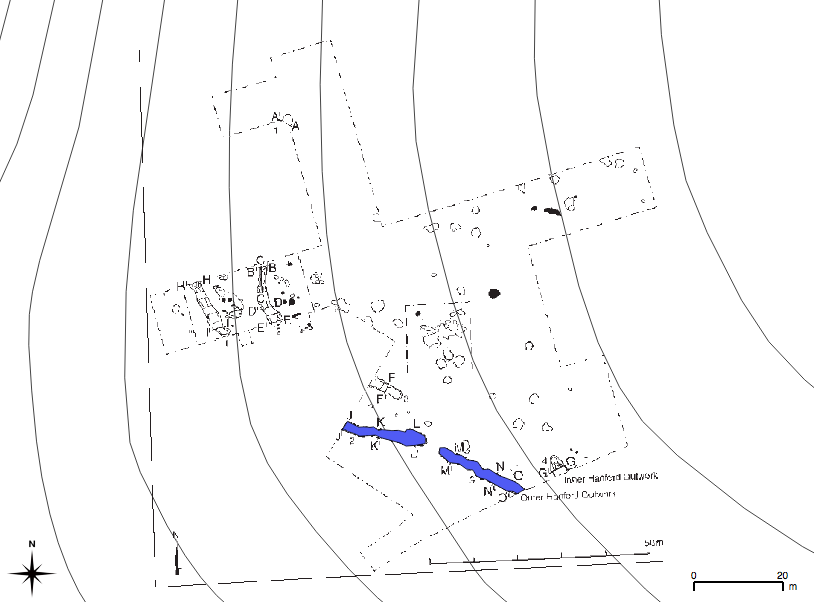
\includegraphics[width=0.9\textwidth]{figures/model6-plan3}
  \caption{Bayesian model for the Hanford outworks, Shroton spur outworks and discrete central area features; and plans of the features dated in the Hanford outwork, from fig 4.13 \citep[144]{Whittle:2011kl}}
  \label{fig:hanfordetc}
\end{figure}

This final section of the bayesian model includes several spatially distinct areas, the Hanford outworks, the Shroton spur outworks and a set of discrete features in the central area.

\begin{figure}
\centering
	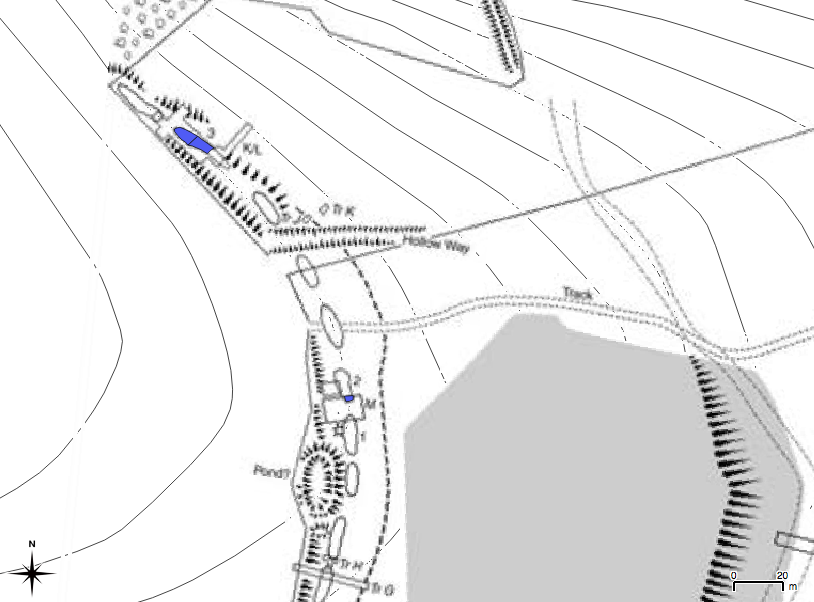
\includegraphics[width=0.8\textwidth]{figures/model6-plan1}
	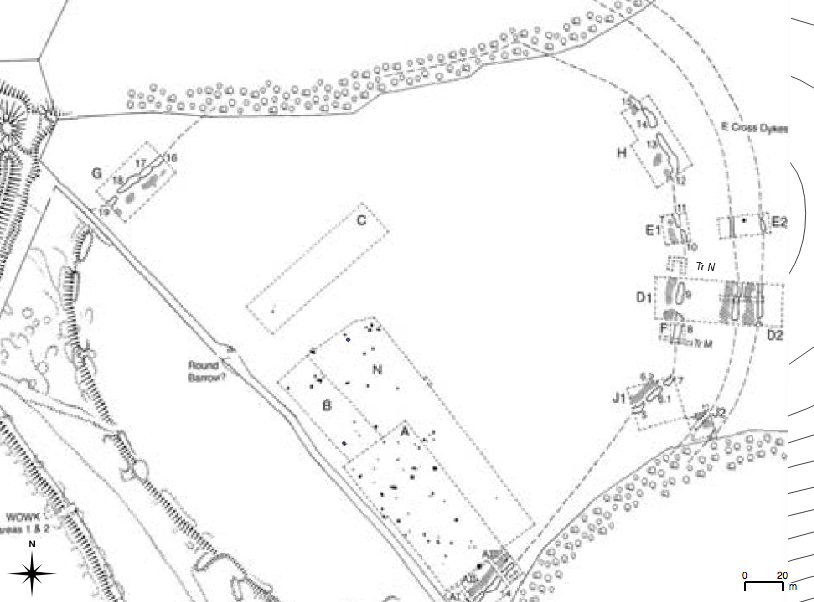
\includegraphics[width=0.8\textwidth]{figures/model6-plan2}
  \caption{Plan of features shown in the model of figure~\ref{fig:hanfordetc} for the Shroton spur outworks and discrete central area}
  \label{fig:hanfordetc2}
\end{figure}

There are a total of four dates from the Hanford outworks, three of which come from segment three, and one from segment two. Of those from segment three, one from charcoal found at the north butt, (HAR-6038) is treated as a terminus post quem as it may pre date the construction \cite[396]{Mercer:2008fk}. The other two are from articulated cattle bone found at the south butt (UB-4271 and UB-4272) that the original report concludes are likely to be very close to the construction date  \cite[397]{Mercer:2008fk}. The date from segment two comes from an articulating sample found at the south butt (OxA-7850) which was significantly earlier in date than those from segment three. The original report suggested three potential explanations for this disparity; that the samples from segment two were redeposited, that segment three underwent a ``radical'' cleaning-out, or that they were built at different dates \cite[397]{Mercer:2008fk}.

Moving next to the Shroton spur outwork, the model in figure~\ref{fig:hanfordetc} shows five samples for phase I, these all come from segment three in site K/L \cite[397]{Mercer:2008fk}. There are no dates from phase II, phase III has dates from both sites. From segment two in site M, are two dates on articulating animal bones, (OxA-7031 and OxA-7032) the rest of the dates in this part of the model come from segment three. This includes an articulating dog skeleton, (OxA-7830) human foot and toe bones (OxA-7102) which may have been redeposited \cite[397]{Mercer:2008fk} and so are treated as a terminus post quem, and several bulked charcoal samples (HAR-2371, HAR-2371 and HAR-2378). Finally there is HAR-2368, which is charcoal from a posthole of a possible gateway that the original investigators believed post-dated the ditch construction \cite[398]{Mercer:2008fk}.

Finally for this section of the model are discrete features of the central area. This is made up of three samples of bulk charcoal, including oak. Because of this they are all treated as terminus post quem \cite[402]{Mercer:2008fk}.

\section{Problems with the chronological evidence and interpretation}
A key argument for the use of bayesian modelling, and in fact many other computational techniques, is that they force us to make our assumptions explicit. In this case, by coding a model which encapsulates those assumptions. But the use of bayesian modelling on Hambledon relies on some other, much more implicit assumptions. Firstly, most of the models group dates from multiple parts of the site, sometimes just nearby segments, but also from separate areas of excavation. This relies on the assumption that the phases used to group those dates are in fact contemporary. It also assumes that the dates we do have are in a sense independent observations on the phase being dated, however this is clearly not the case. In many areas multiple dates are taken from the same context, and yield very similar results, clearly material found spatially and contextually close is often temporally close as well. There are a small number of times when this has not been the case, and such outliers are then often modelled as redeposited, so do not add much to the model. While such correlation may seem obvious, it is largely obfuscated in the current bayesian model where dates from, for example, multiple ditch segments are combined. The lack of clearly recorded find spots also makes the investigation of this type of pattern in the data more difficult and less exact. Fundamentally this will lead to those contexts that have been dated more providing greater influence over the bayesian model, and the subsequent interpretation of the site, than those which have less dates (and infinitely more than those with none). There is likely to be spatio-temporal autocorrelation within the data, due to local affects, for example, of deposition, taphonomic processes or excavation. This raises the question, how appropriate is it to combine data across parts of the site (subject to their own local affects) within the bayesian model? Secondly, the dates provided by the bayesian model are not large in number, but they have been used to provide dates for the whole series of earthworks across the site, in their entirety, clearly this is based on a similar assumption, that undated areas must also follow the same sequence of phases, occurring at the same time as those in the excavated areas. While the reliance on these assumptions may be required in order to provide a best effort temporal model of the data, they should be made explicit, as otherwise there is a risk of over using the data to draw inferences, about areas of the site that it cannot support.

\subsection{The Central Area}
The central area is the part of the site with the greatest quantity of dating evidence, the models shown in figure~\ref{fig:central1} and figure~\ref{fig:central2} are split by segments, although apart from segment nine, these are in two groups. Segments five to seven form one group, and segments 16 to 19 form the other. These two groupings are of a series of adjacent ditch segments, and so, if the physical evidence of the fills that make up the different phases supports them being combined, effectively into one segment (for the purposes of the model) this is not particularly controversial. However in some cases this may not be accurate, for example while the stratigraphy segments 17 and 18 is very similar, the dates may tell a different story. The date of an articulating sample, UB-4269, is significantly later than dates from the same phase of fills (phase III) from segment 17 (OxA-7022, OxA-7023, OxA-7099). The original report puts this down to UB-4269 being in an undetected re-cut, but also raises the possibility that the sequences were not contemporary \cite[399]{Mercer:2008fk}. 

The grouping of dates for segment five to seven only contains dates for phase I, while the grouping for segments 16 to 19 contains a deeper chronology. More problematic, perhaps is the comparison of one side of the circuit to another, a visual inspection of the original model and resultant dates could be a starting point, but unfortunately the scales used for both sections of the models are different, making this more problematic, although it would appear for example that the phase I dates for segments 16 to 19 are possibly slightly earlier than those on the other side of the circuit. When we consider their location, on opposite sides of the circuit, this would make sense, what is more surprising is that this appears to have been omitted in the original analysis of the chronology.  In order to further investigate this point figure~\ref{fig:central-phasei-model} has been generated from the original data. This shows the start boundaries for each of the segments, or groups of segments from the central area, as grouped in the original model. Once on a standard scale, it is possible to easily compare the start dates form ditch segments on either side of the circuit. Clearly the main peak of the three distributions is broadly similar, with that for segments five to seven being the most constricted, while segment nine has a broader probability, and segments 16-19 being in between the two, in terms of size of date range. The peaks in probability for segment nine and segments 16-19 are slightly later than that for segments five to seven. In terms of dates the start of segments five to seven boundary is modelled at 3660 B.C. to 3630 B.C. (68.2\%) and 3680 B.C. to 3570 B.C. (95.4\%), segment nine is 3650 B.C. to 3540 B.C. (68.2\%) and 3660 B.C. to 3530 B.C. (95.4\%), and segments 16-19 is 3650 B.C. to 3595 B.C. (68.2\%) and 3655 B.C. to 3570 B.C. (95.4\%). Clearly there is a possibility that all three sections of the causeway were constructed at around the same time, however this new output from the model demonstrates this is far from certain. Interestingly this analysis brings to light that the distribution for segment nine and segments 16-19 are more similar than that for segments five to seven and segment nine, despite the close proximity of segments five to seven with segment nine, and segments 16-19 being on the other side of the circuit. This is most likely to be an artefact of the underlying uncertainty, rather than evidence for sequencing to the ditches initial construction, as there is still significant overlap between all three, especially at the 95.4\% confidence interval.
There is very little further comparison that can be done between the north-west and south-east sides of the enclosure as so few phases are dated for both sets of segments. Phase III is a possibility, but there is very little after that from segment nine, on the south-east side, where as to the north-west there are several dates for phase IV and VI.

\begin{figure}
\centering
	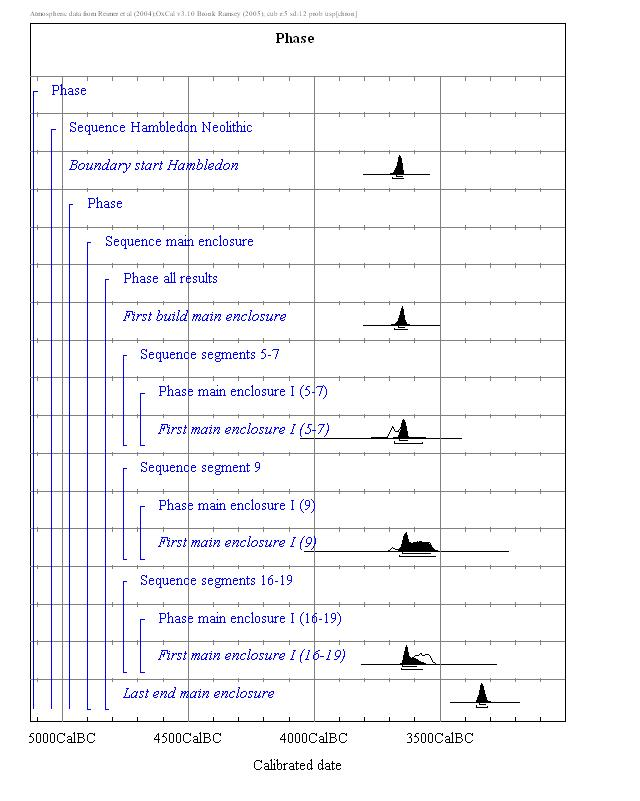
\includegraphics[width=0.9\textwidth]{figures/central-phasei-model}
  \caption{Posterior density estimates for the start of phase I in the ditch segments of the central area of Hambledon Hill}
  \label{fig:central-phasei-model}
\end{figure}

\subsection{Cross Dykes and the Long Barrow}
The cross-dykes are a prime example of a very different problem, a simple lack of data. The outer east cross-dyke only provides one date to the bayesian model, one which has been argued could come from an extension \citep[401]{Mercer:2008fk}. All that can be stated with any confidence is that after this date, segment E2 of the outer east cross dyke existed. The inner east cross-dyke is a little better, all of the dating evidence is for the first phase, so the model provides a clear date of initial construction of the cross dyke, or at least of segment four, where four out of five dates came from. It would appear that these dates are ever so slightly earlier than those for the initial construction of the central area, but this is not noted in the earlier studies. A complete lack of modelled dating evidence for any subsequent activity on the east cross-dykes means it is not possible to make any more temporal comparisons with the central area. 

The south cross-dyke suffers in much the same way, here there are dates preceding the construction, and dates of later recut activity, but nothing to date the original cutting of the ditch. An estimate for cross-dyke construction is obtained via the model, however this ignores the fact that the pre cross-dyke activity was towards its western end, whereas the later activity was more central. It assumes that construction of the cross-dyke was a fairly rapid event, rapid enough that the later recuts must have taken place after the cross-dyke had been constructed along its full length to the west. 

The south long barrow is a different case, the excavated quadrants are all close by or adjacent to one another, and there are a fair number of dates, particularly for phase I. Like the central area, the dates for phase I, and the sequence for the barrow assume that phases are comparable across the quadrants. In this case that would seem to be a fairly likely scenario, although it is possible that different sides of the barrow may have been cleared at different times. As the dates for phase I all came from one quadrant and the dates for phase II, III and IV all came from another different quadrant, and the excavation report contains no indication of a synchronous sequence, there is no clear dating evidence either way. 

\subsection{The Stepleton Enclosure}
The model for the Stepleton enclosure and outworks is very different to that for the central area, this model is not separated out by ditch segment, meaning its accuracy relies on the sequences of its segments being synchronous. Unfortunately, the excavators could not be sure that this was the case \cite[394]{Mercer:2008fk}. Part of the problem is the lack of dating evidence for each phase, and the lack of sequences of dates in any segment. The result is a sparse model that combines data, where there is a clear lack of evidence that the data should be being combined. The phase I section of the model contains samples only from segment three, so we can be confident that these provide a date around the time of its construction, but there are no dates for the construction of any other segments. So to assume that the date from the model for `first build Stepleton enclosure' is applicable to the enclosure in its entirety is, at best, optimistic. The discrete features in and near to the enclosure are included in the model, but as they are included in a phase they have little to no effect on the overall model, and only act on other dates within their phase. 

The outer Stepleton outwork has only one date, which provides a broad potential range for the digging of the butt of one segment. The middle outwork suffers the same problem as the enclosure, in that a sequence of dates is built up from dates coming from multiple segments, the results of which are extrapolated across the whole outwork. There are also very few dates, for example for phase III there is only one. The inner Stepleton outwork has a greater number of dates, but does suffer from the same issue of combining dates from multiple segments in the same part of the model, in this case five segments. The reference to the middle outwork, which is modelled as earlier than the inner outwork is, in fact, modelling that segment six of the middle outwork pre-dates a set of pits, which are in fact not in its vicinity, or near the closest section of the inner outwork. In particular, the samples for phase III were statistically significantly different \cite[395]{Mercer:2008fk} which may be down to the slow rate of accumulation of the fills, or it may be that the four samples came from three segments, which did not have a synchronous sequence. This is clear evidence that the spatial locations for the source of dates in bayesian models should be considered, as this does offer an alternative explanation to the one from the original report.

\subsection{The Hanford Outworks}
The plan for the Hanford outworks suggests a significant part of it has been dated, unfortunately the dating evidence is very thin. The dates are separated by ditch segment, but all the dates would appear to come from close to the base of the ditch, so there is no sequence as such, assuming the segments are contemporary. The date taken for the initial building of the outworks is almost solely influenced by the two dates from the south end of segment three. With the terminus post quem from the north end of segment three and the date for segment two having little impact on the first build date, even though the date for segment two is significantly earlier. The model in this case appears to be reflecting one of the original reports interpretations of this earlier date, that the dated material in segment two is redeposited. While the three potential interpretations have clearly considered the spatial evidence, in so far as they suggest the two segments might have had different use lives, either one being much more recent, or the other having had a substantial clean out. These segments are very close, which would make it seem less likely they had such different use lives, however the plan in figure~\ref{fig:hanfordetc} does show that the two segments are on substantially different alignments. This evidence would favour the suggestion that segment three was a later addition to the outworks. However when an alternative version of the model was run, as shown in figure~\ref{fig:hanford-remodelled}, with the sequence for segment three included inside another sequence, to indicate a strict ordering following segment two, the agreement index values fall so low that clearly with the evidence we have, such a strict ordering is not supported. For example UB-4272 falls down to 0.9\% from 61.6\% in the original model. A clear benefit to the bayesian modelling approach is that it allows for such experimentation and the construction of alternative versions of reality. In this case, we can rule out (based on current evidence) one such potential version of events, and must assume instead that either the sample from segment two was redeposited, or segment three underwent a radical clear out.

\begin{figure}
\centering
	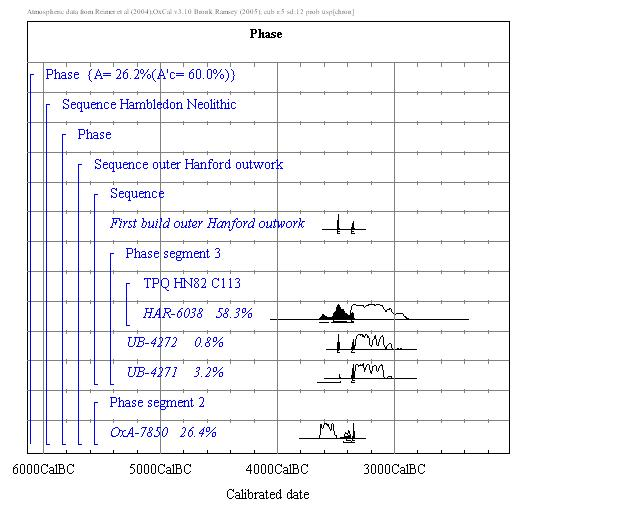
\includegraphics[width=0.9\textwidth]{figures/hanford-remodelled}
  \caption{Posterior density estimates for an alternative model of the Hanford outworks, where segment two pre-dates segment three.}
  \label{fig:hanford-remodelled}
\end{figure}

\subsection{The Shroton Spur Outwork}
The Shroton spur outwork model takes dates from two excavation areas, and as with other models, combines them into one component of a sequence block, assuming that the phases are comparable. And the computed first build date, calculated from only a very small part of the outwork, is assumed to be representative of it as a whole. While the dates may show a good agreement index when placed in the model in this way, the model should ultimately be guided by the archaeology, and not the computed agreement index. The dating evidence for the Shroton spur is ultimately a sequence of the earliest phases from a single ditch segment, plus two corroborating dates from similar fills in another segment. This is not really enough to suggest a unified construction, and lacks dating evidence from any later activity.

\begin{figure}
\begin{center}
	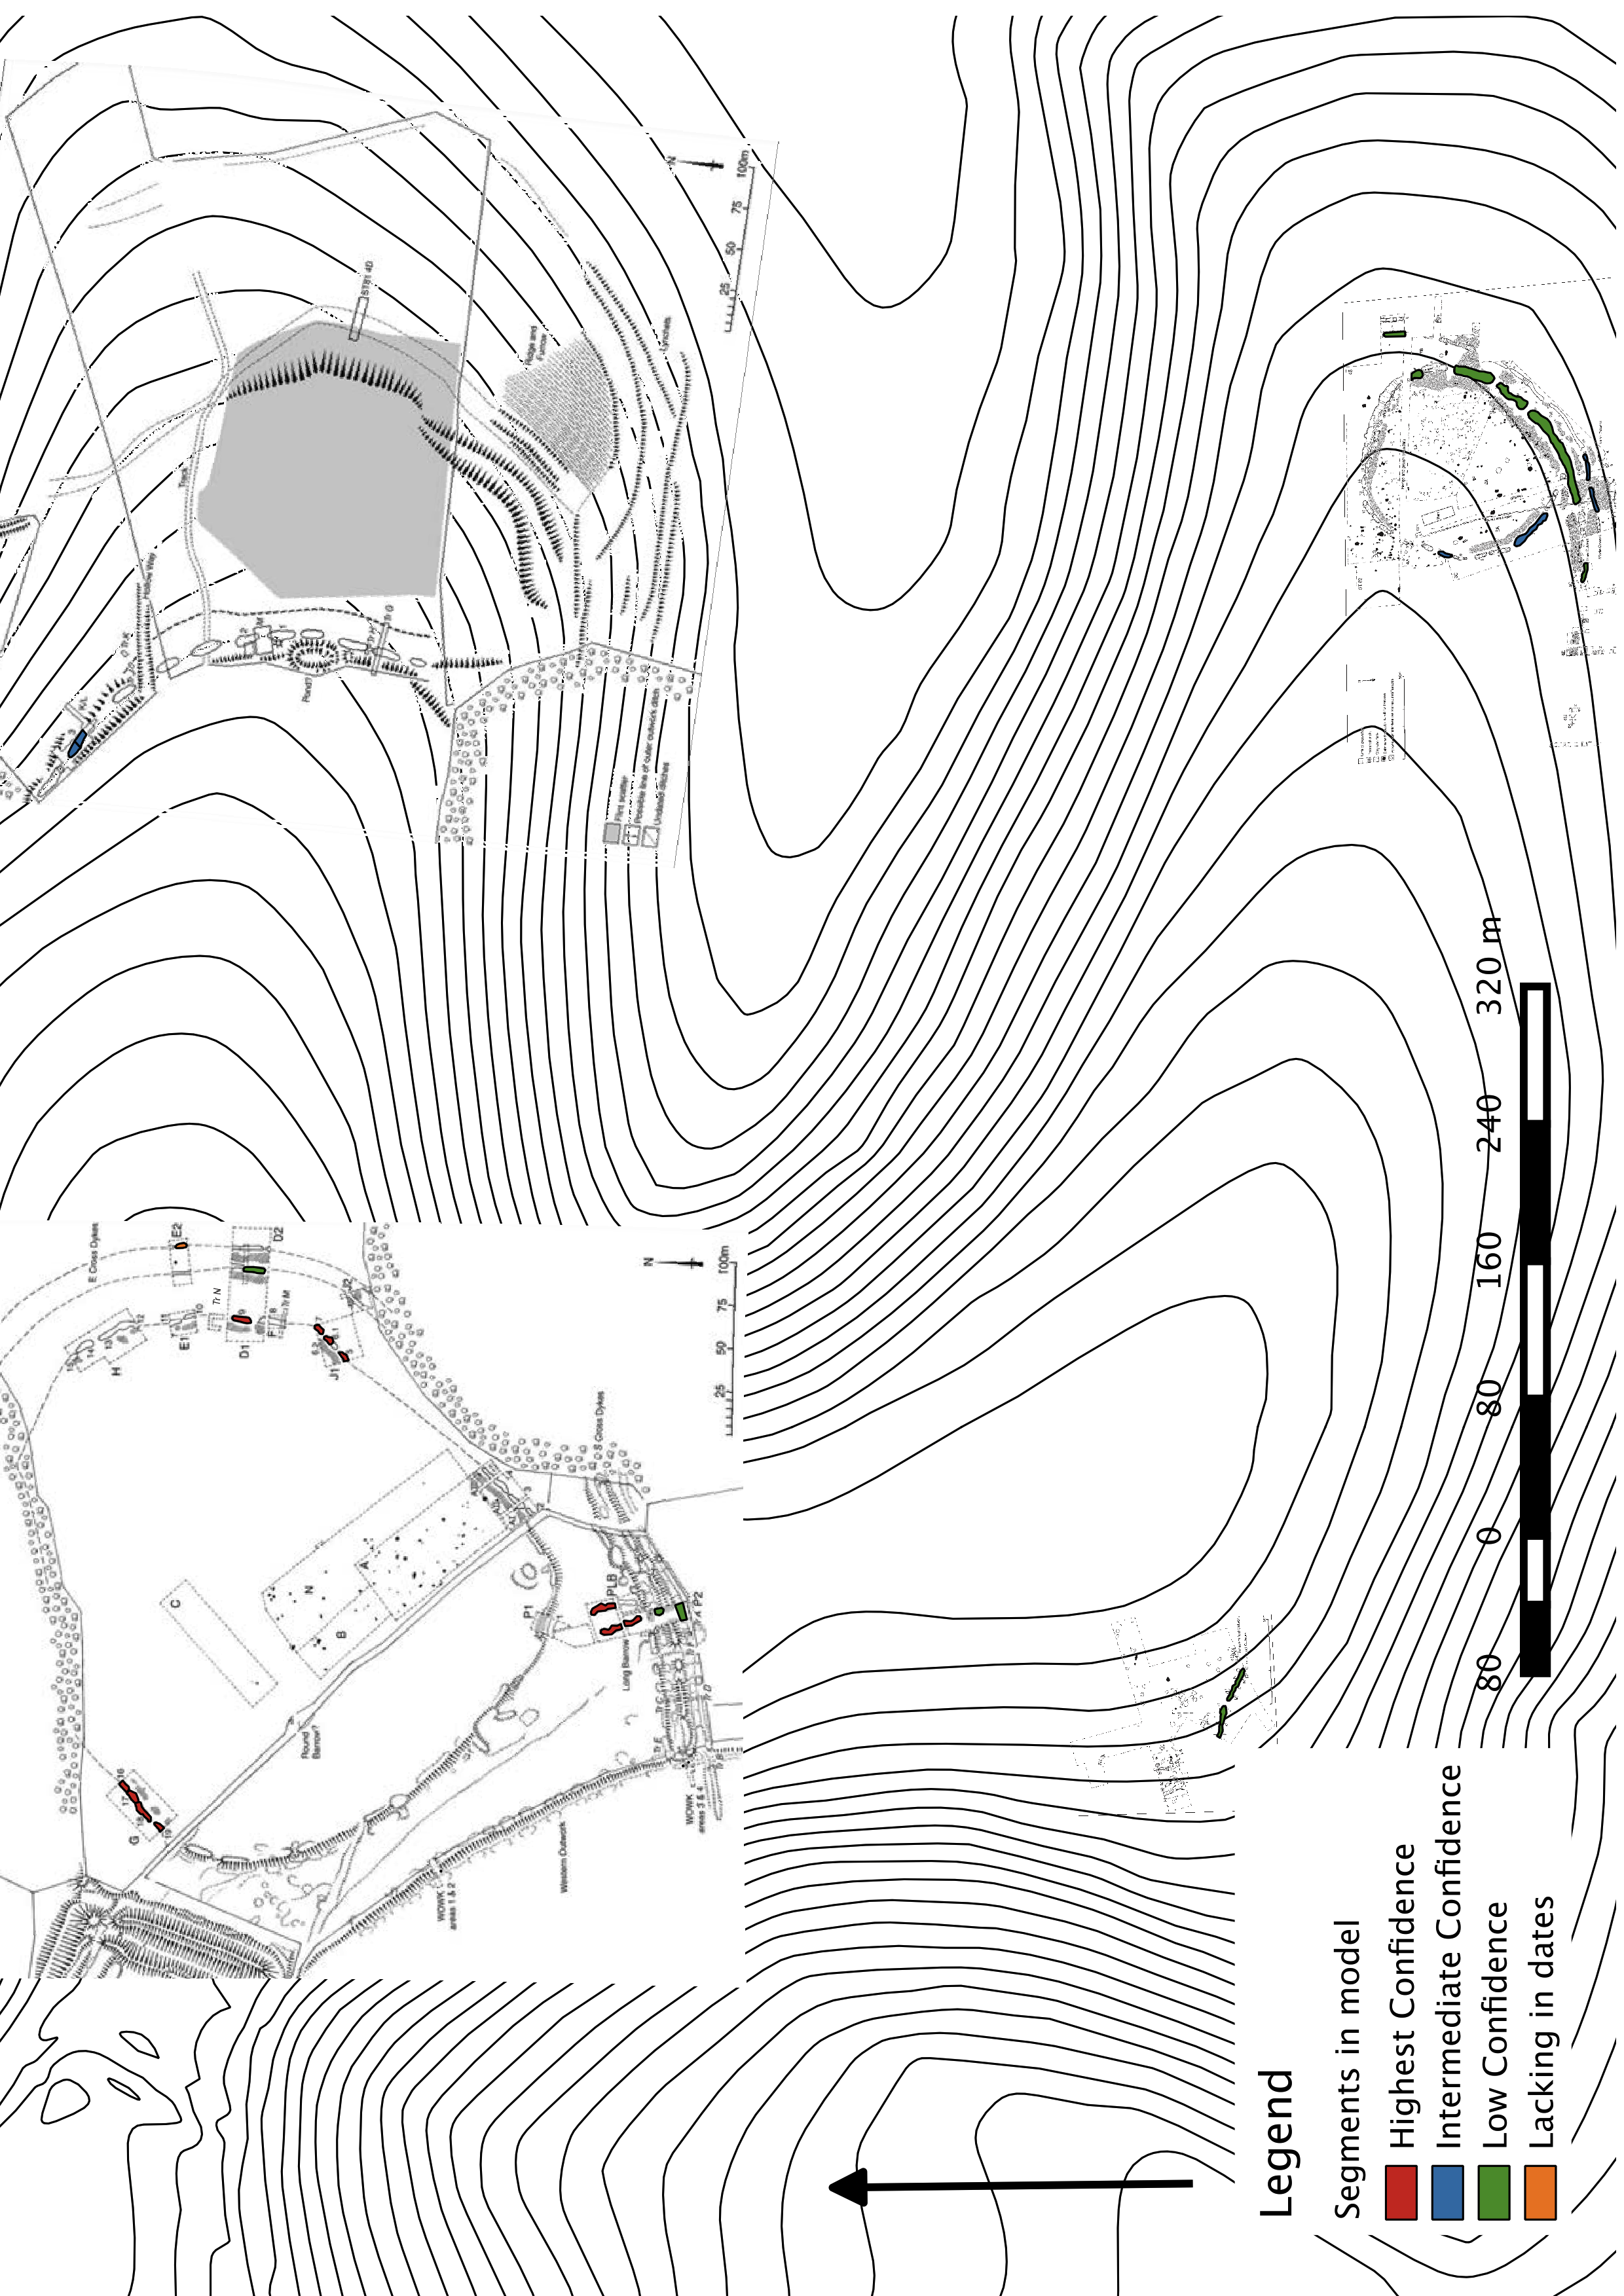
\includegraphics[width=0.9\textwidth]{figures/dated-confidence}
\end{center}
  \caption{Plan of segments included in the bayesian model, by qualitative confidence interval}
  \label{fig:dated-confidence}
\end{figure}

\subsection{Confidence in the interpretation}
In conclusion, the chronological evidence varies across the site; in some areas the models more accurately reflect the spatial nature of the evidence, while in others dates from relatively distant segments are combined as though they were found side-by-side. Clearly the kind of joint spatial and temporal model display, as shown above, aids the spatio-temporal interpretation of the evidence, enabling the archaeologist to easily assess whether there may be spatial issues with a bayesian model. The review above has also shown that a bayesian model does not capture all of the uncertainty around a defined chronological model of the archaeology. Additional key uncertainties around the comparability of phases remain implicit, as does the applicability of a model across un-excavated areas. 

It is possible to rank the confidence of the model across various parts of the site, based on the descriptions above. Such a ranking is clearly qualitative. The areas falling into the highest confidence bracket have a set of dates for a particular segment modelled in a chronological order,  in this case only the central area fits that requirement. The next group would be those dates that have one but not both of these, e.g. a set of dates in order, but from multiple segments, or a very limited number of dates from a single segment. Into this set fits: the south long barrow, Stepleton enclosure, middle Stepleton outwork and Shroton outwork. The low confidence areas those where there is some doubt over the validity model, following a consideration of the spatial evidence this group includes: the inner east cross dyke, south outworks, inner Stepleton outwork and the Hanford outworks. And the final group is those areas simply lacking in dating evidence: the outer east cross dyke, western outworks, outer Stepleton outwork and isolated pits in the central area. This grouping of segments is displayed in figure~\ref{fig:dated-confidence} and in figure~\ref{fig:dated-confidence-buffer} with a 10m buffer. 

\begin{figure}
\centering
	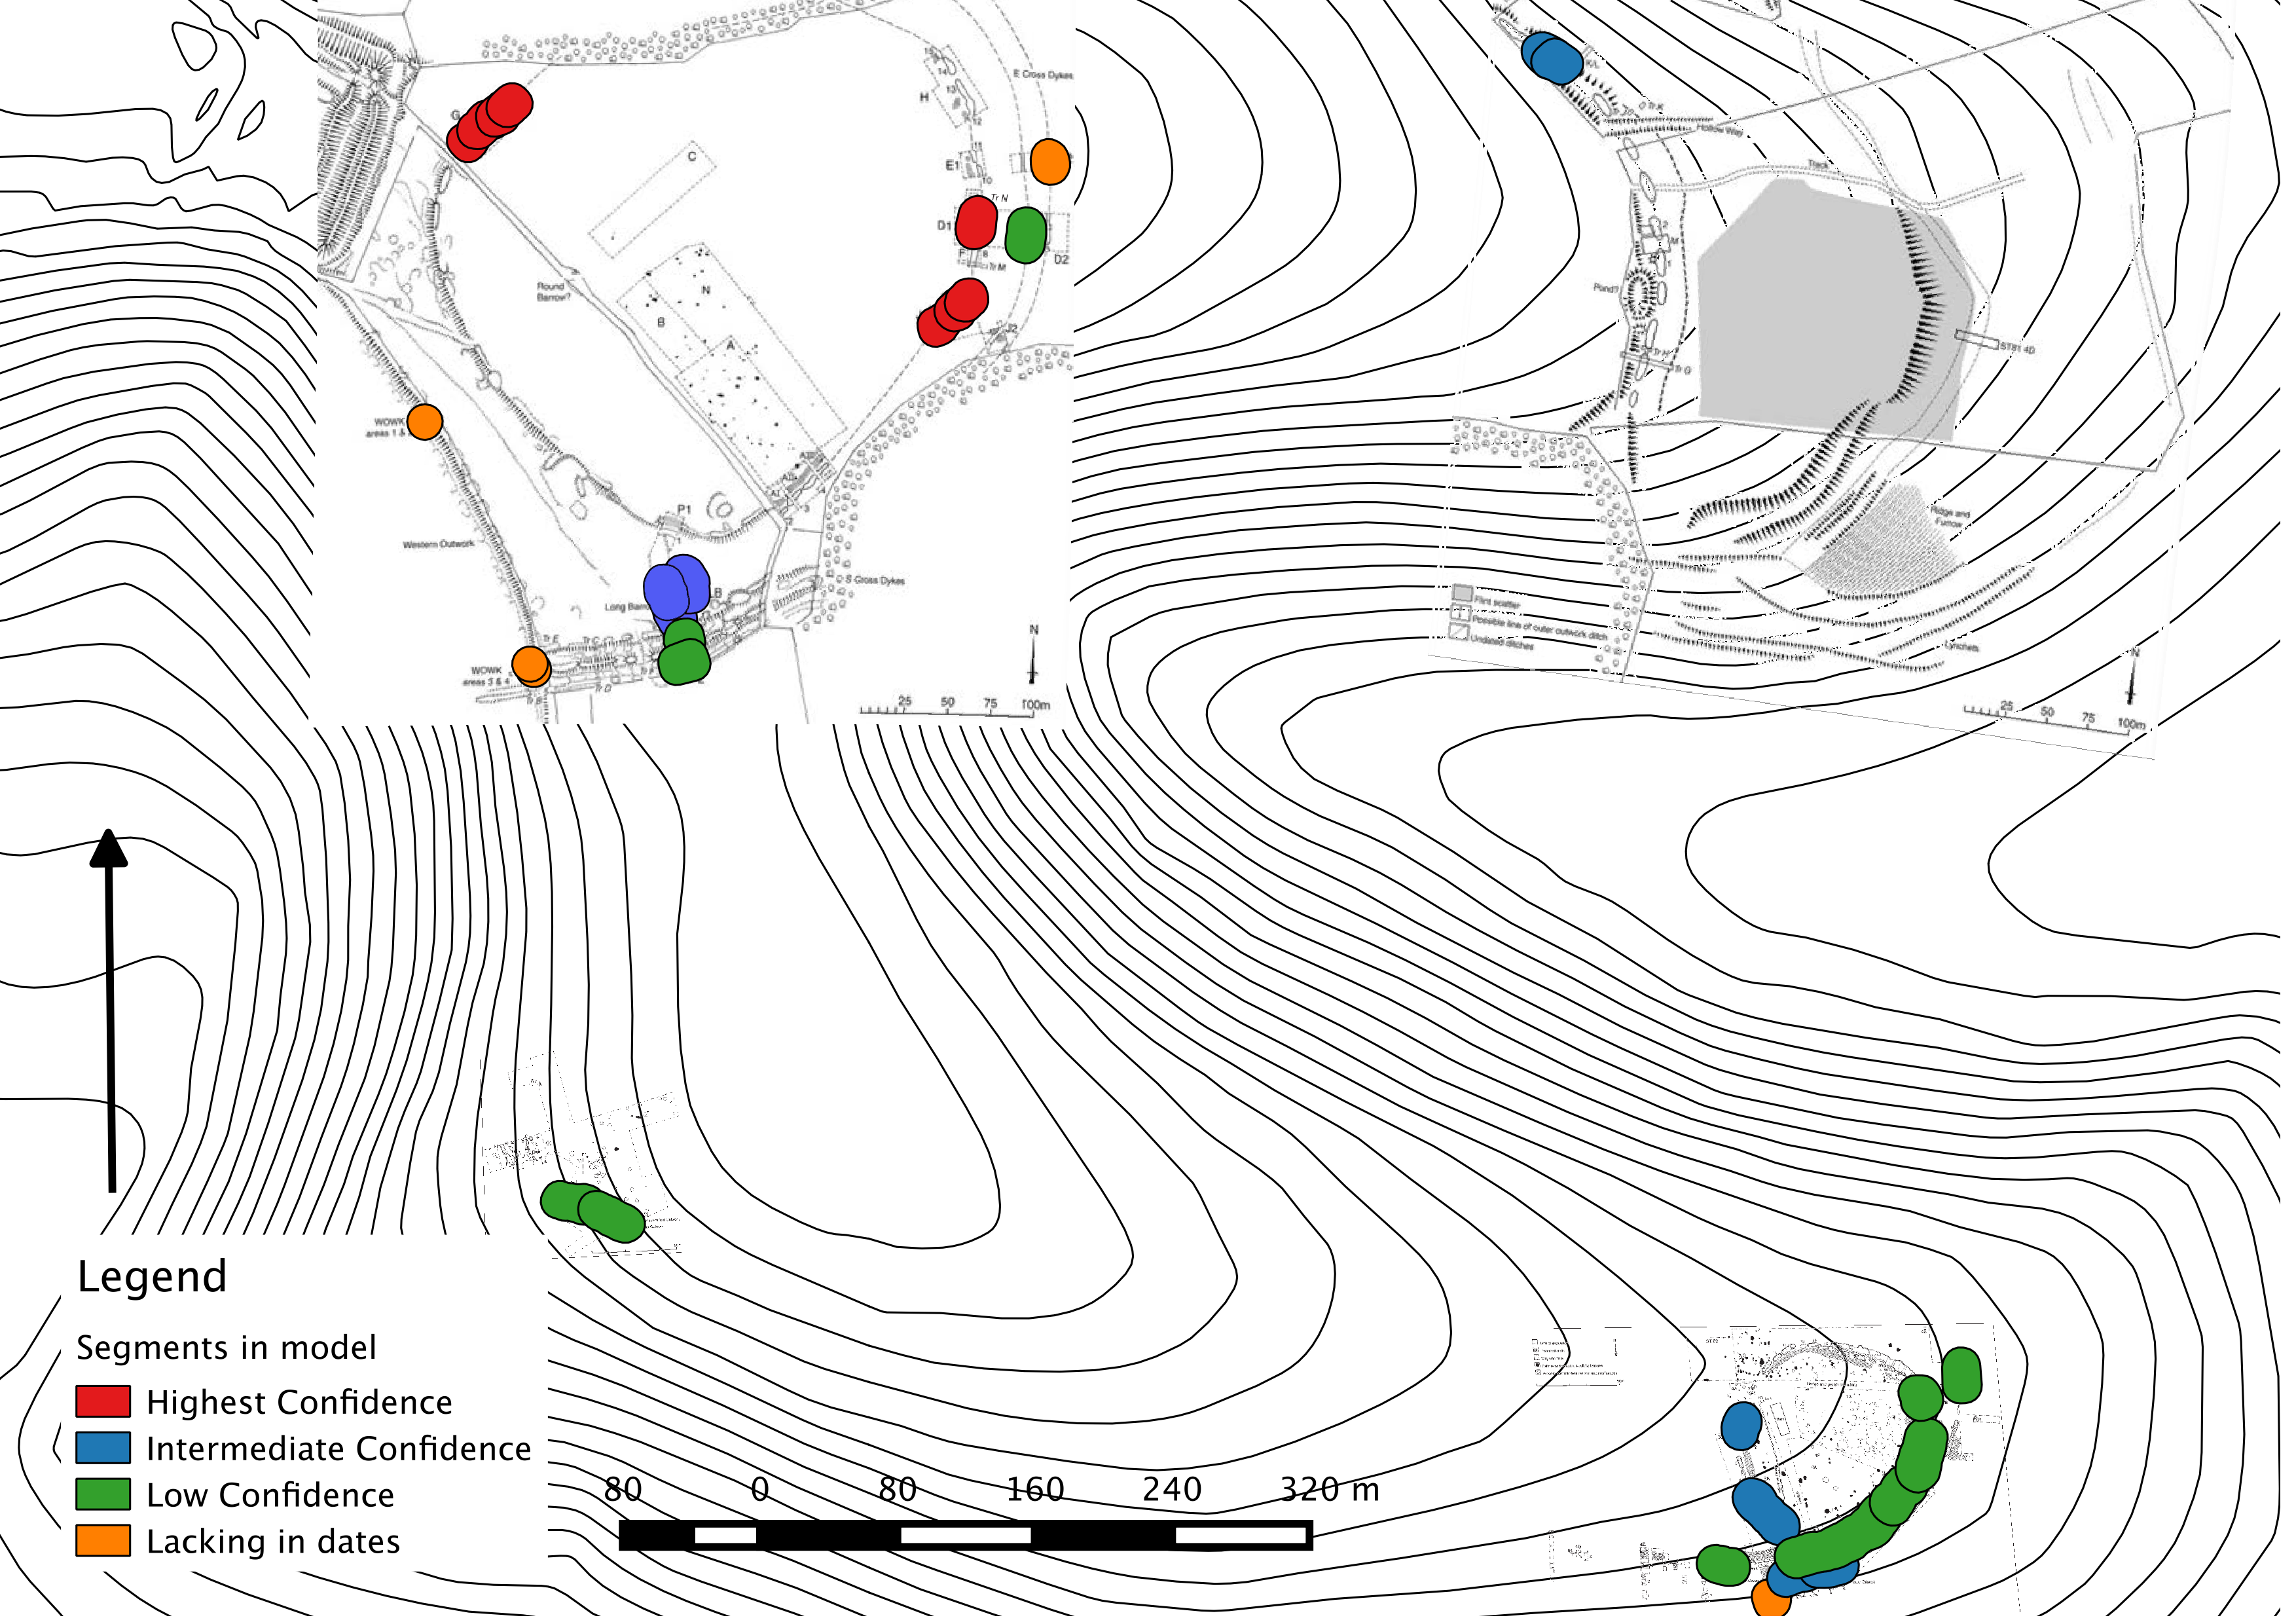
\includegraphics[width=0.9\textwidth]{figures/dated-confidence-buffer}
  \caption{Plan of segments included in the bayesian model, by qualitative confidence interval, with 10m buffer}
  \label{fig:dated-confidence-buffer}
\end{figure}

Clearly the focus for any chronological or temporal interpretation of the evidence should be focused around these areas. An arbitrary 10m has been applied for figure~\ref{fig:dated-confidence-buffer} to aid visual identification. If we accept the implicit assumptions of the bayesian model for Hambledon Hill, that un-excavated areas are likely to have the same sequence of fills as excavated, then we may consider surrounding ditch segments to take the dates from those in the bayesian model. However the extent to which this might be applicable is impossible to accurately asses without excavating those areas. For areas that have been excavated, but provided no dating evidence, if it is possible to provide evidence that the dated fills were synchronous, we can transfer the dates with some confidence, as is done in almost all of the models of Hambledon Hill. In this case the areas of assumed dates, should adopt a confidence level below that of the original area.

These limitations with the temporal evidence have all been highlighted by a combined spatio-temporal review of the data and bayesian analysis. Having reviewed such limitations in detail, the next step is to further investigate the benefits of combined spatio-temporal analysis, in particular quantitative analytical methods.

\section{Quantitative Analysis}
The spatio-temporal distribution can be further investigated using a variety of quantitative techniques to formally asses the distribution of dates from Hambledon Hill across space and time. The results of such methods must be considered carefully as they can hide a variety of complexities with the data and assumptions in the method itself. There are a wide variety of spatial statistical methods from which to choose, many of which are provided as part of modern GIS packages, however such methods are not necessarily applicable to radiocarbon dates. In order to use such standard techniques, it is necessary to approximate each bayesian modelled radiocarbon date as a single value, it is these values which will be used to compute the statistics. 

Approximating a radiocarbon date can be done in a variety of ways, for example an average, such as the mean or median; or by selecting a date at random from within the distribution, with or without weighting the choice using the dates underlying distribution; or some other esoteric method for approximating the value. In many ways this choice is arbitrary if the goal is to find the `best' approximation, as there is no way of evaluating the accuracy of the selected value. The best we can do is identify a good approximation, taking reasonable account of the underlying probability distribution.  

In order to simplify the process and focus on the methods of analysis (rather than the method of approximation) averages from the probability distribution will be used as the approximate value for the subsequent analysis. The original bayesian analysis was undertaken using version 3 of OxCal, which produces a mixture of binary and text file output. To simplify extracting the averages (as calculated by OxCal) a one time transformation was undertaken as part of this project, using the following process:
\begin{enumerate}
\item The model was extracted from the OxCal 3 project, HHall.14i file, which contained the full model
\item This model was then imported into a new OxCal 4 project 
\item The OxCal 4 project was evaluated
\item A custom script is used to extract the averages from the OxCal output .js file
\item The averages are added to the shapefile of radiocarbon sample locations
\end{enumerate}
Due to the nature of the calculation process this has resulted in some values being slightly different than the values used to up this point.

\subsection{Moran's i}
A suitable technique for this data set is Global Moran's i. As a broad measure it can provide valuable summary statistics over the whole data set, with the potential to follow up using more fine grained techniques. As a measure of spatial autocorrelation when applied to the date values over the whole study area it will generate a statistic that indicates whether like values tend to group together spatially, be distributed randomly, or to be far apart. There are a series of variable parameters for the calculation of Moran's i as implemented within ArcGIS, the first being the feature value. OxCal produces two averages, the mean and the median vaules of the calibrated date probability distribution. Due to the simplicity of extraction and calculation it seems reasonable to perform the analysis using each. The next parameter is the conceptualisation of spatial relationship, the ArcGIS documentation \protect\citep{ArcGIS:fk} states that the inverse distance methods are appropriate to model processes where the closer two features are in space, the more likely they are to interact/influence each. As we are attempting to assess the spread of sample values across the site that could be influenced by past activity, taphonomic processes, research bias and recovery methods, the assumption that closer features are more likely to interact than farther ones is fair. The next parameter is distance method, either euclidian or manhattan - euclidian was used for all analysis, as manhattan is not appropriate in this context. The distance threshold was set as the extent of the dataset, so all points would influence all other values, as there is no obvious arbitrary value which would be applicable across the site. 

The ArcGIS tool also allows customised weights to be specified as a conceptualisation of spatial relationship. Clearly there are many potential ways of using it. A relatively simple option is a boolean weight on a per feature basis, so this would mean that each date has a weight of one for all other dates from the same feature, in this case mostly pits or ditch segments, and 0 for everything else. This effectively means that all dates from the same feature heavily influence one another, compared to those between features, however it removes the spatial distance between features as a component of their relationship, it also does not consider the stratigraphic relationship.
Removing the spatial distances is not a particular problem, as the features are all fairly small in size, and the locations given within the GIS are only approximate, in fact for many of the dates the only location provided in the report is a feature name, so an equal weighting of within feature dates is not an unreasonable assumption.

\csvautolongtable[
  table head= \caption{Results of calculating Moran's i to evaluate the extent of spatial autocorrelation between each dated sample across the Hambledon complex}\label{tab:moransi} \\\hline
               \csvlinetotablerow\\\hline
               \endfirsthead\hline
               \csvlinetotablerow\\\hline
               \endhead\hline
               \endfoot,
]{figures/moransi.csv}

The results from the different combinations of averages and conceptualisations of spatial relationship are summarised in table~\ref{tab:moransi}. The crucial piece of information is provided in the conclusion column, which is that for all of the combinations the results do not appear to be significantly different to a random distribution. This is an interesting result as it has already been shown that the bayesian models have spatial issues, in particular that it is unusual for a feature or segment to provide a set of dates that are spread throughout the chronology. A good example being the central area, where most of the dates for the early phases come from one side of the enclosure, and those for later phases from the opposite side. This is likely due to two main causes, firstly the averages used hide a wide degree of variability caused by the random effects of radiocarbon dating, calibration and bayesian modelling. Secondly the dates used come from a bayesian model, they were selected to provide a depth and breadth of time, so a lack of spatial autocorrelation is an indication that the model has been well constructed. The results clearly reflect positively on the construction of the model, although clearly there are concerns that have not been identified by this statistical method, most likely due to the average being used as input data.

\subsection{Stratigraphic Distance}
The weighting or relationship values used so far have been based on spatial distance between dates. While the method has not been entirely a-temporal, the weighting between two dates has not incorporated any form of temporality. When considering a purely spatial weighting between the dates, there is no autocorrelation - the distribution of average date values is indistinguishable from random. In order to incorporate some temporality the stratigraphic distance can be used as a source for a custom conceptualisation of space. This would give dates that are stratigraphically closer to one another a greater weight than those which are stratigraphically more distant. Applied over the whole site this would remove any spatial component from the weighting, however the boolean per feature weighting can be combined, including a limited spatial component, of whether dates are from the same feature or not, in the weighting. There is no Harris matrix diagram for Hambledon Hill, which would be the obvious starting point for creating such values, this leaves the layer numbers, and associated sections as the source for stratigraphical information. Of course this stratigraphic data has already been transformed into a model for the bayesian modelling process, the bayesian model therefore can provide a source for the stratigraphic relationships between dates. While this model is an abstraction from the raw data, it also incorporates an interpretation, putting the dates in an order. It is this ordering that will be used to create a value for stratigraphic closeness. OxCal has two methods of grouping multiple dates, by sequence and by phase. Dates within the same phase are assumed to belong to events which occurred concurrently, where as sequences are events that occurred in the specified order. These can be nested, so often there will be a sequence of phases. An inverse distance approach can be used to transform this into a numerical value, where the value is the inverse of difference in the order of a sequence between two dates. Dates within a phase can be assumed to be concurrent, and so given a relationship value of one.

The depth (vertical distance) between finds was not used as different fills had different depths of content, and so this distances does not provide a reliable measure of how dates relate to one another chronologically. However neither chronological distance nor vertical distance provides a consistent and reliable measure of how far apart temporally the two samples were deposited. One possibility would be creating a combined chronological and spatial autocorrelation weight, however the reason this has not been done for Hambledon is the plotted locations of dates are estimates, in most cases it was simply the ditch segment. In other cases they were plotted on diagrams in the original report, but combining these with those where only a very rough location was available would imply a false sense of accuracy. The spatial component of the weight must be such that it can logically be combined with the stratigraphic component. Due to the fact that most of the locations are only at the level of the feature, using the exact x and y c-ordinates of the plotted locations creates a false sense of accuracy. As a result of this the most compatible representation of space is probably the boolean weight per feature, as this will asses whether the date value distribution within features, weighted by stratigraphic distance is distinguishable from random. 

\csvautolongtable[
  table head= \caption{Results of calculating Moran's i using two custom conceptualisations of distance between each dated sample across the Hambledon complex}\label{tab:moransi2} \\\hline
               \csvlinetotablerow\\\hline
               \endfirsthead\hline
               \csvlinetotablerow\\\hline
               \endhead\hline
               \endfoot,
]{figures/moransi2.csv}

The results for using a purely stratigraphic weighting and a stratigraphic weighting combined with a boolean per feature weighting are summarised in table~\ref{tab:moransi2}. The two different models demonstrate two different representations of the ``distance'' between dates. In a purely stratigraphic representation the spatial locations of the dates are not factored into the weighting of relationships between the dates. The very strong positive autocorrelation is not unexpected as it is simply stating that similar dates occur closely within the bayesian model. By augmenting this representation of distance with the spatial data the Moran's i statistic can be used to confirm the observation above, that groups of dates within the bayesian model, usually comprising a phase section, cluster spatially. 

The clustering of dates demonstrated in table~\ref{tab:moransi2} confirms the observation above, that groups of dates cluster spatially. But it does not provide any indication of the cause of that autocorrelation, It could be that the results are entirely due to the random nature of the radiocarbon method. It could be that the positive auto-correlation is down to the construction of the model, in inclusion of specific results, or the way samples were chosen to be dated. Or it could be that activity on the site clustered in certain areas, during certain times. This was the conclusion of the analysis of the bayesian model, so it would be fair to conclude that the positive auto-correlation is also the result of this. Like the bayesian model multiple models can be constructed and compared, in this case of different methods of weighting relationships between the date values. That the weighting based solely on the bayesian model showed a very strong likelihood of clustering of date values is not a surprise, this shows that those dates modelled as from the the same part of the chronology tend to have similar values, compared to those that are not stratigraphically close. Perhaps more of a surprise is that when the weighting is modelled as solely spatial the distribution is indistinguishable from a random distribution, even when using the boolean weights within feature measure, which might have been expected to have shown some evidence of clustering. 

What this means is that it is not possible to say that date values show any evidence of spatial autocorrelation, when dates from the whole duration of the sites use are included equally. Put this way, it is perhaps less of a surprise, different areas of the site will have been a locus of activity in different times, and may have gone in and out of focus (and then back in again). As the biographical approach reminds us, sites often have rich histories of use and re-use, re-interpretation and it would perhaps be naive to expect such a broad measure as Moran's i to show spatial autocorrelation of date values over a site with such a rich history. So while it might be not much of a surprise that combining a spatial model indistinguishable from random and a stratigraphic one that is very strongly clustered would lead to a less strongly clustered result, it is in fact a very important outcome. Its true significance is in demonstrating the value of combined spatial and temporal analysis, showing that across the whole site, throughout its use, date values are likely to cluster chronologically, within features. As mentioned before, this supports the observation above, that certain sections of the bayesian model's chronology come from distinct areas and very few areas provide a chronological vertical section through the model. The result of this is that sequences are built with dates for different phases coming from different features.

\subsection{Local Measures}
Clearly if there was a more accurate way to approximate the dates to a single value, this would potentially make the use of Moran's i more valuable. It is also worth considering local statistical measures as these will be more focused on a subset of the results. Two such measures, with the potential to add value are Getis-Ord Gi* and the Anselin Local Moran's i as the presence of hot spots and clusters or outliers of feature (i.e. date) values is highly likely.
 
\subsubsection{Anselin Local Moran's i}
A standard measure of local spatial association, it is included in ArcGIS as a method to generate an output feature class containing identification of clusters and outliers. Figure~\ref{fig:cluster-hh} and figure~\ref{fig:cluster-lh} show the results of running this analysis using the combined chronological and spatial custom conceptualisation of space, with boolean feature values. Using either the mean or median date values identified the same dates as clustering and outliers, so only the output for the mean is shown in the figures here.

\begin{figure} 
\centering
	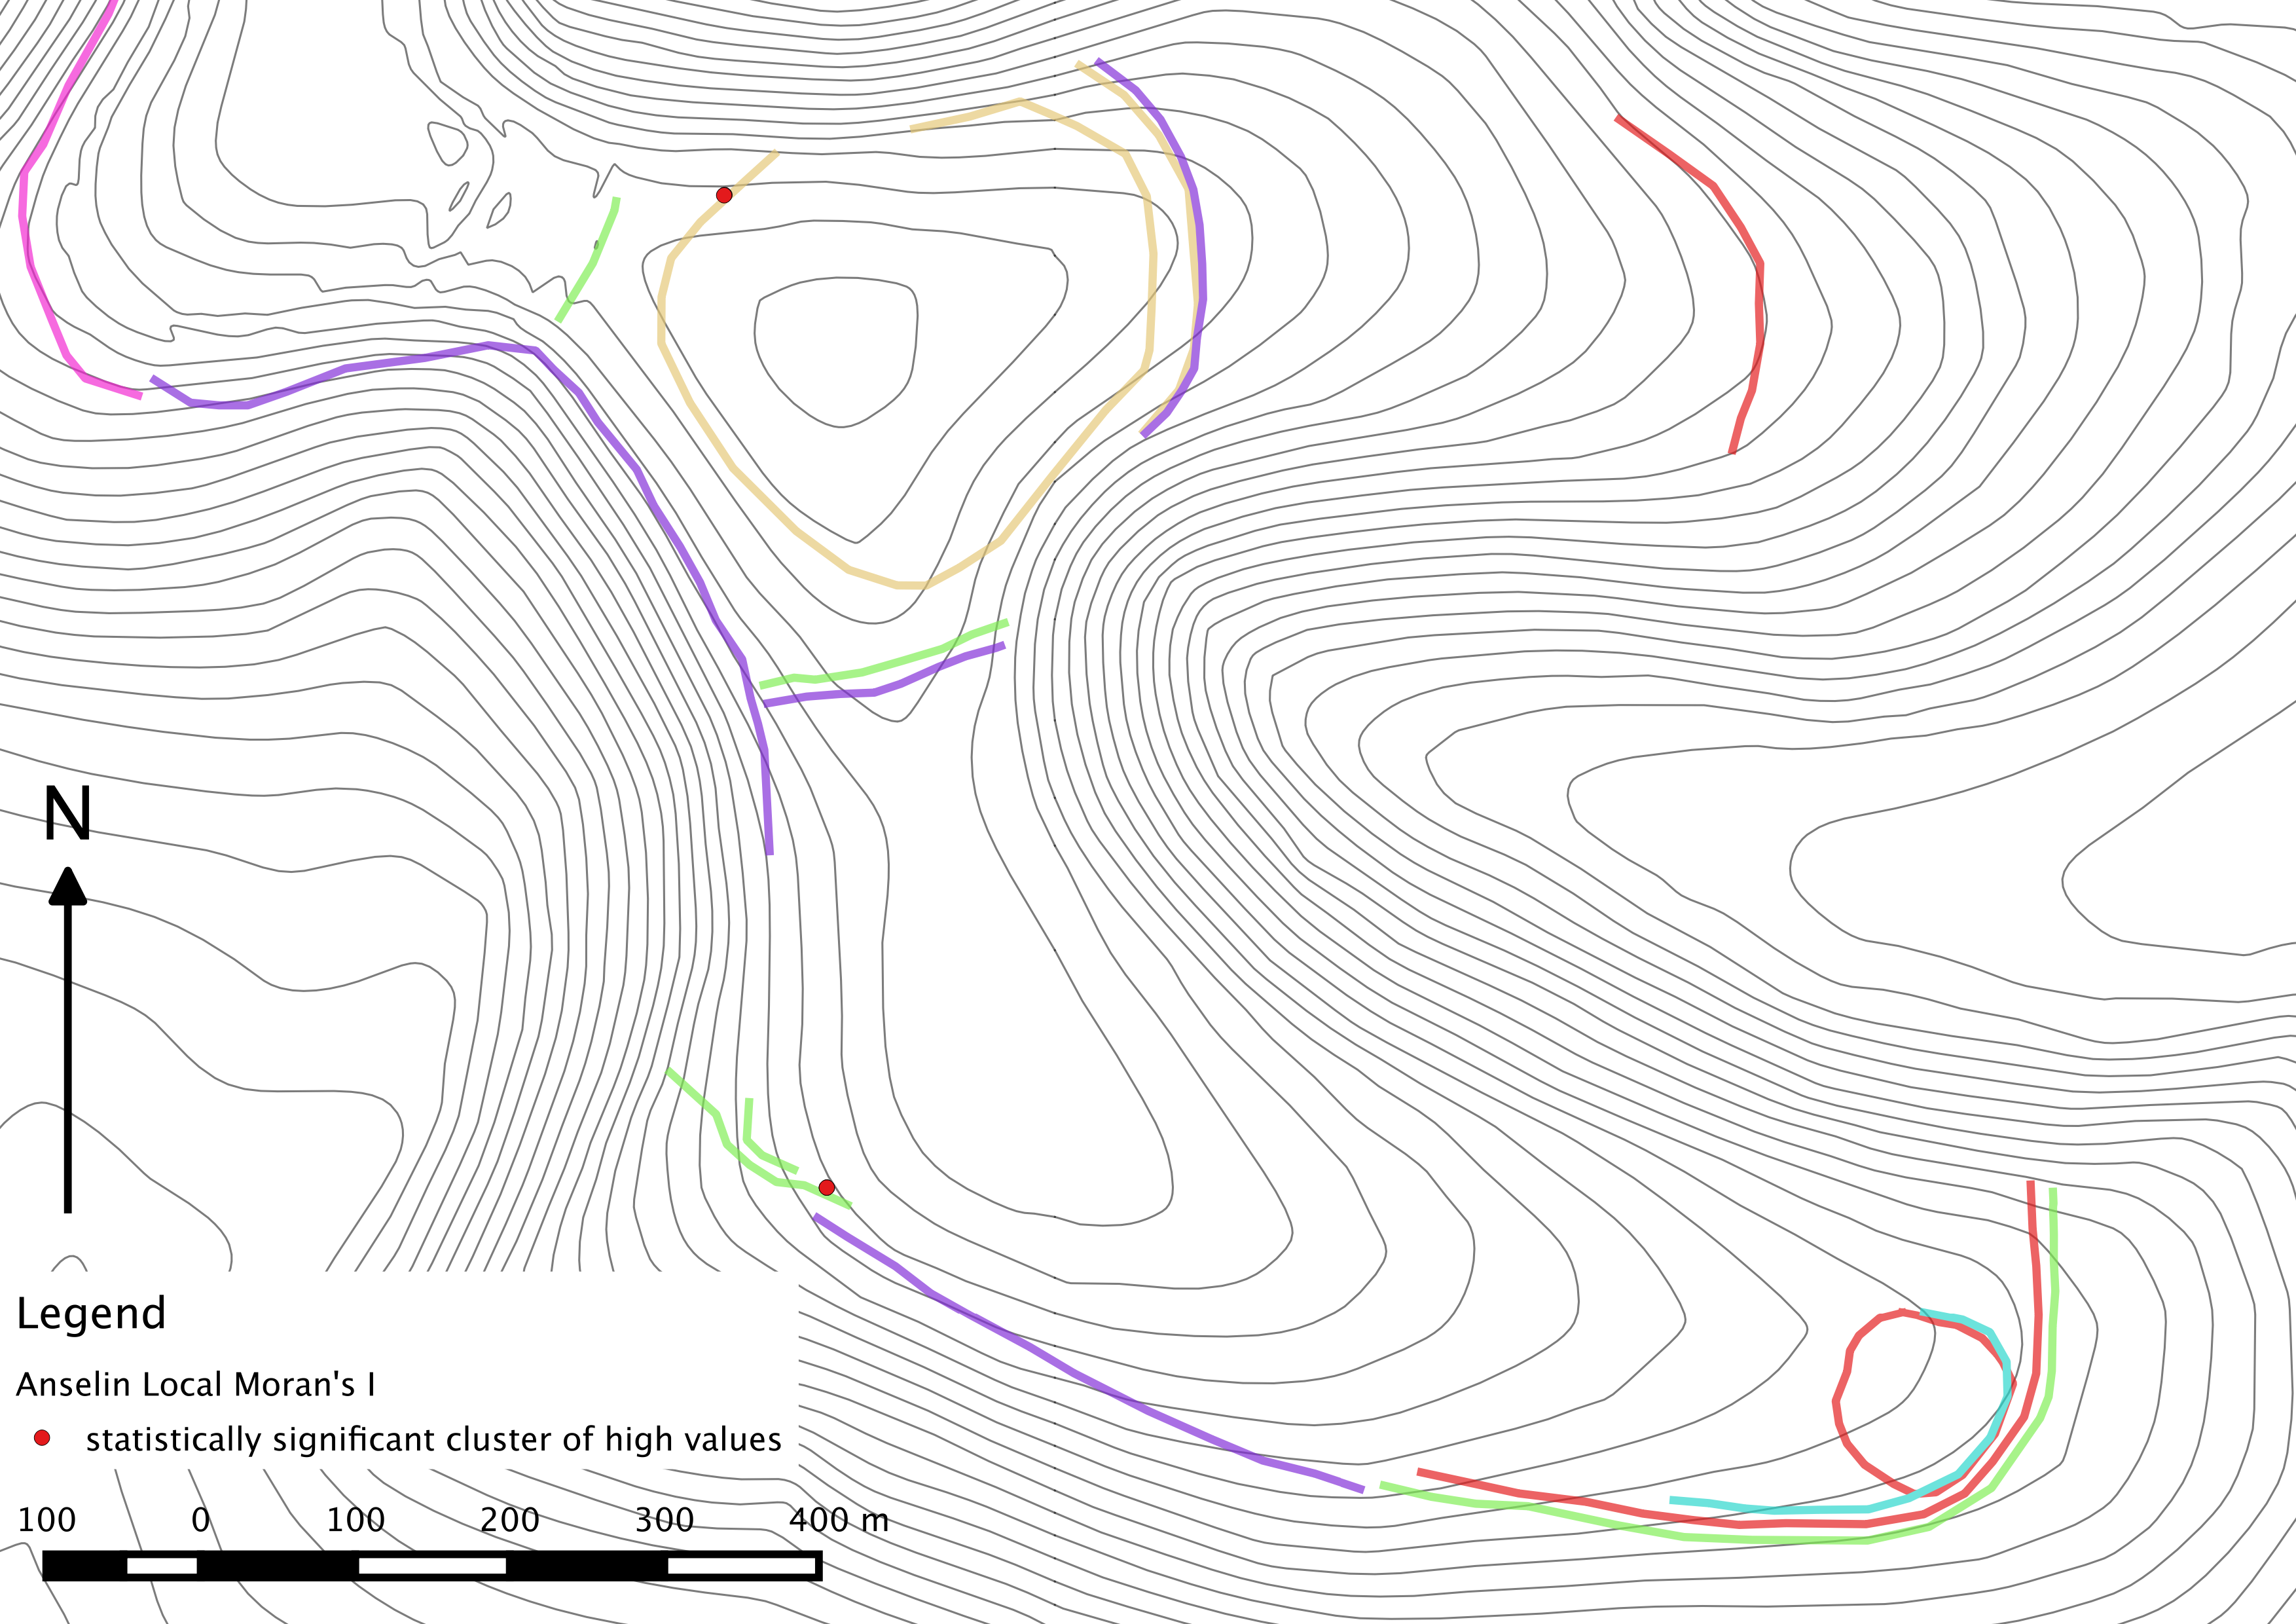
\includegraphics[width=0.9\textwidth]{figures/cluster-HH}
  \caption{Plan of statistically significant clusters of high values}
  \label{fig:cluster-hh}
\end{figure}

\begin{figure} 
\centering
	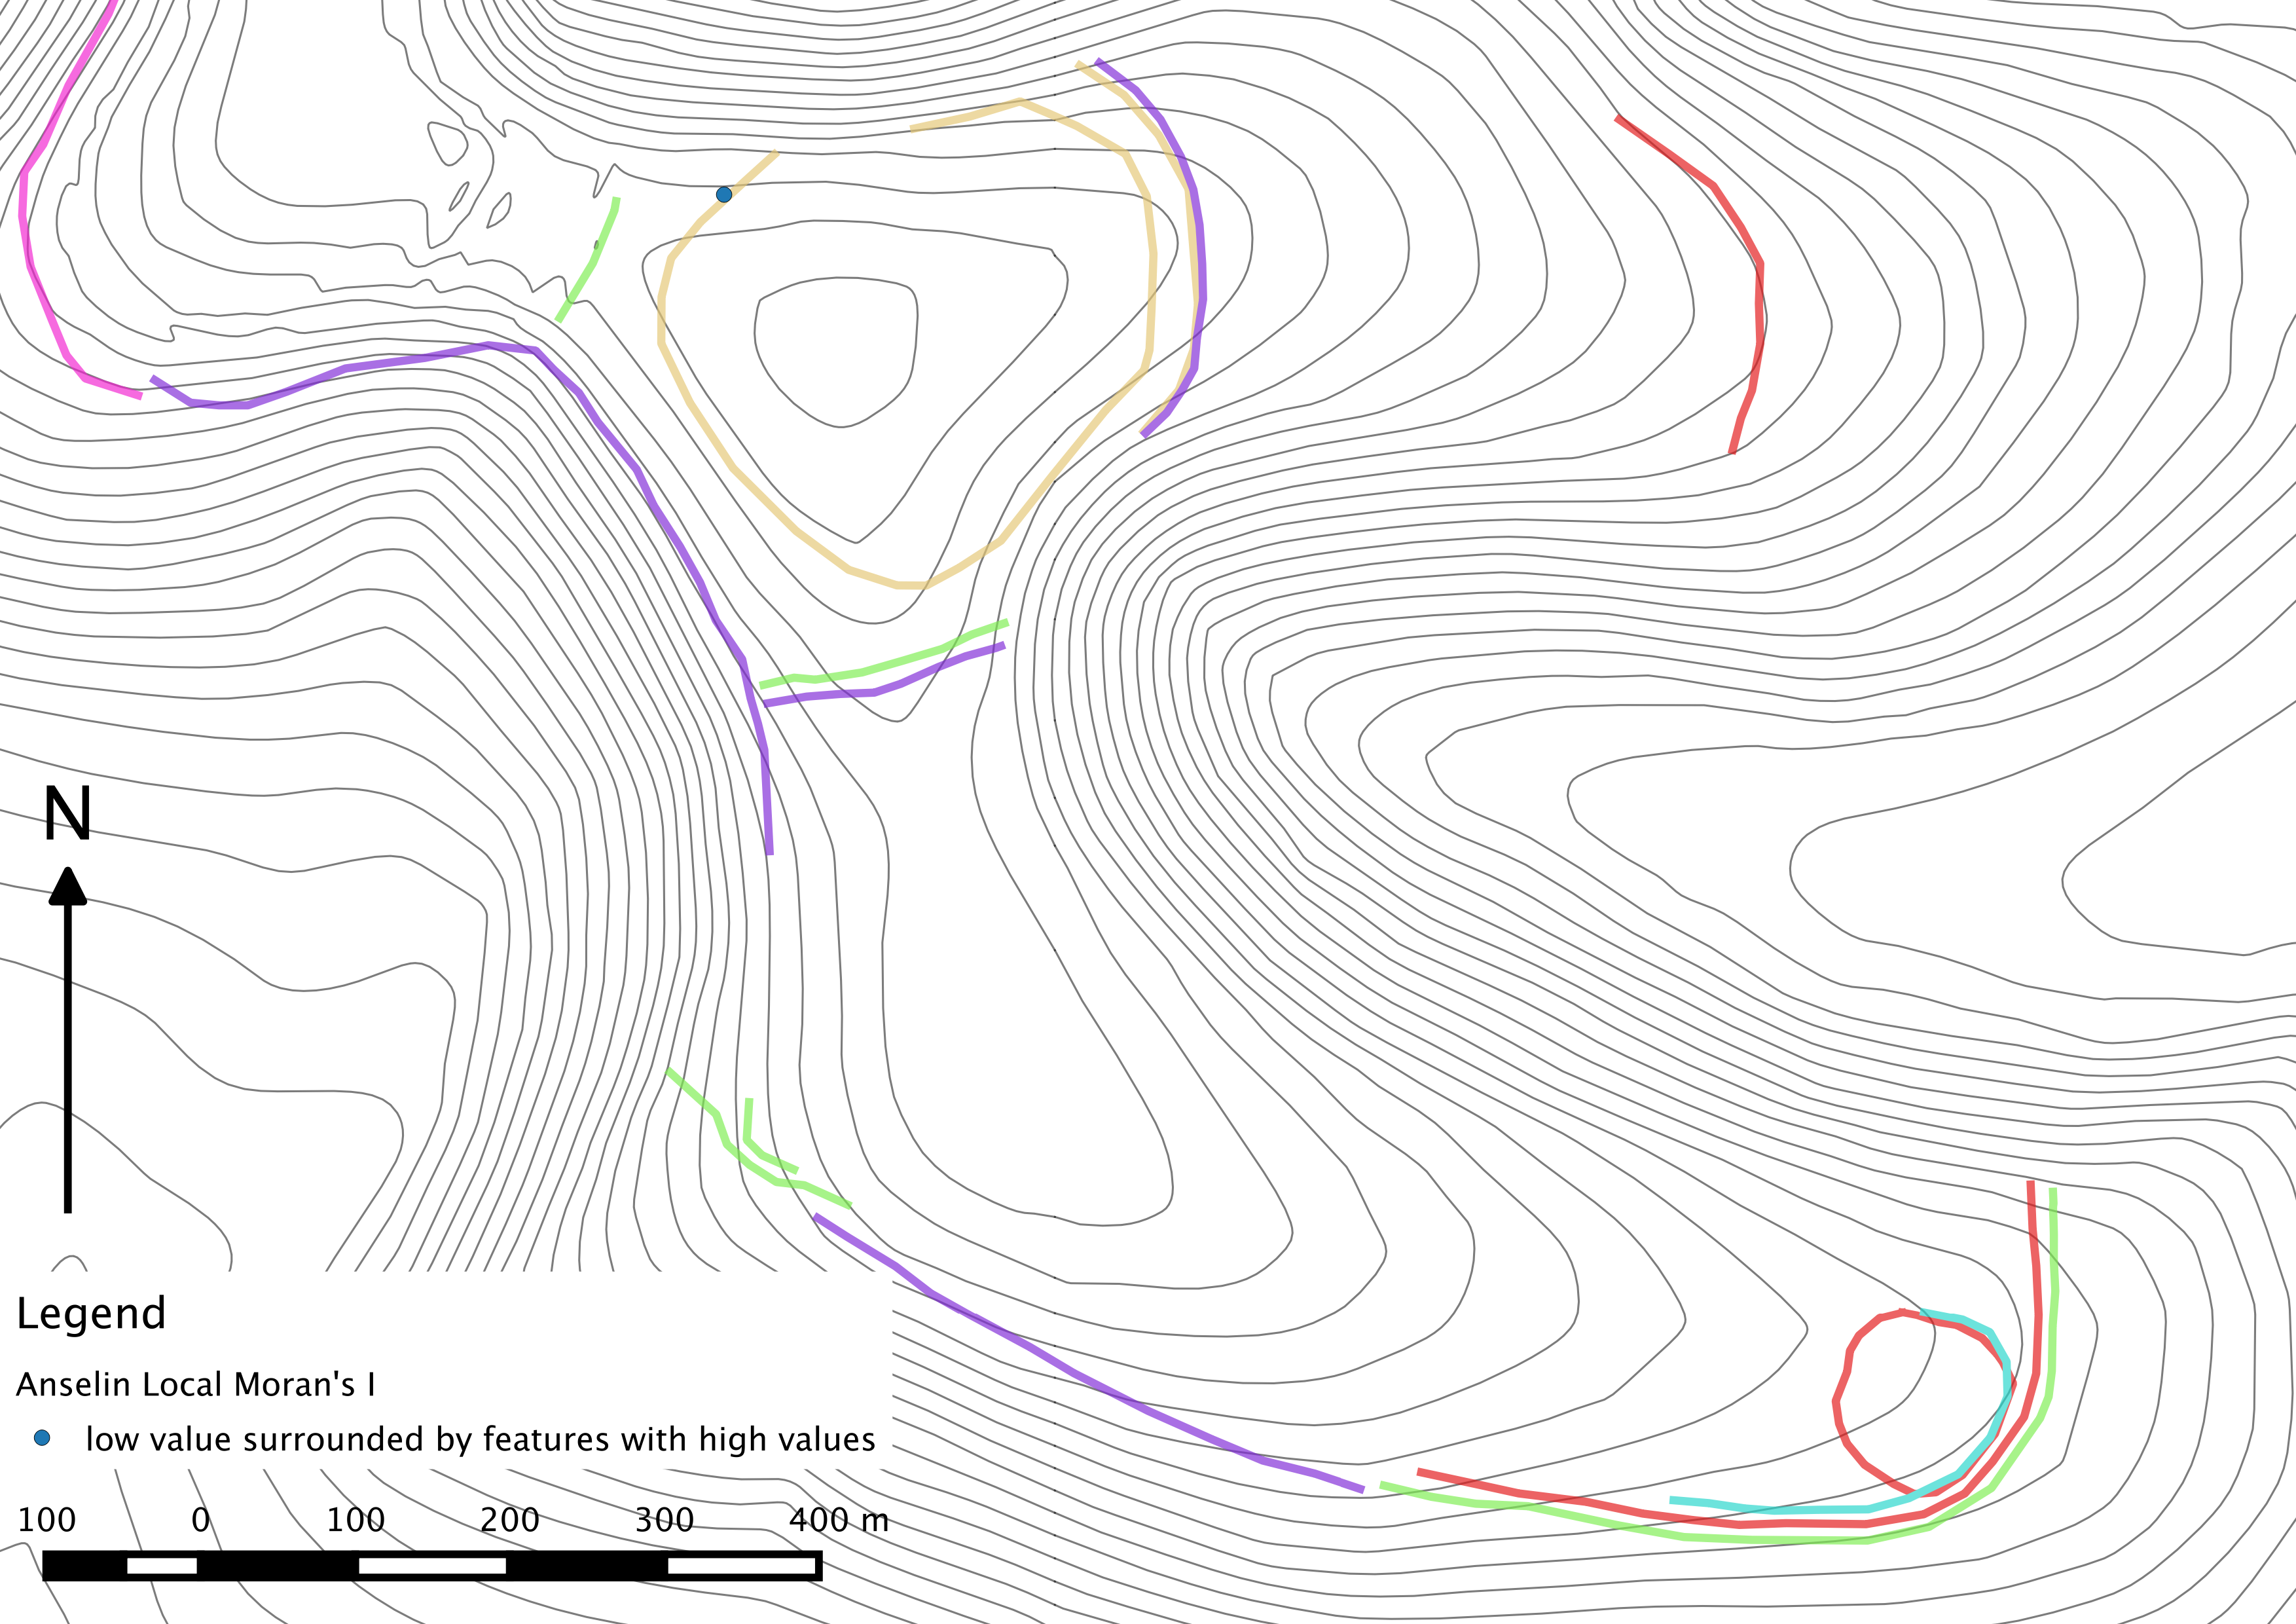
\includegraphics[width=0.9\textwidth]{figures/cluster-LH}
  \caption{Plan of statistically significant low value outliers}
  \label{fig:cluster-lh}
\end{figure}

The statistically significant clusters of high values shown in figure~\ref{fig:cluster-hh} are in two locations, the north west side of the central enclosure and the east side of the Hanford outworks. From the central area, in segment 17 dates OxA-7039 and OxA-7040 are replicates of the same sample. From this ditch segment there are a total of 14 dates, from ten samples, that came from four contexts, it accounts for a large portion of the bayesian model from this part of the central enclosure. Chronologically the dates span four phases, from phase III, through phase IV and phase VI to phase post-VI. Such a relatively even spread through the chronology makes this hotspot a good candidate for further investigation.

The model, reproduced in figure~\ref{fig:central2}, shows how close the dates are across these four phases. While the averages used for the clustering algorithm are falsely accurate, the modelled dates would suggest a period of around 200 years to have elapsed between the first dates (OxA-7099 and HH76 2808 - if we ignore the bulked HAR-2370) and last (HH76 3046) with the last two phases occurring relatively close together and phase IV having the most uncertainty. While conclusions are clearly limited in spatial scope, they provide a snapshot into the activity at this part of the site over a relatively small time scale. The original report describes the phase III fills as occupying the bulk of most segments \cite[56]{Mercer:2008fk} and notes that in segment 17 it is marked by concentrations of articulating animal bone, this fill in some areas began accumulating very soon after the ditch was cut and in was in some places recut. The two samples from this phase being so tightly dated (e.g. OxA-7099 modelled as 3586-3529 cal BC at 95.4\% probability) is perhaps partly due to them coming from the same dump of animal bones. It is clear from the model that the following phase IV deposits are dates of an ashy deposit, dumped into a centre of a sub-segment, described as ``extensive"  \cite[56]{Mercer:2008fk} and rich in cultural material. The dates from this phase have greater uncertainty, with the probability distributions covering a larger time frame. It is perhaps not surprising that phase V fills are not present in the model of segment 17, as these are described as material resulting from individual small scale episodes of activity, and a thin silt layer \cite[56]{Mercer:2008fk}. By phase VI, less than 200 years after phase III, the ditch is now a ``shallow depression'' \cite[56]{Mercer:2008fk} into which a series of slots were cut, and possibly organic containers placed, containing varied cultural material, in segment 17 the bones and flint protruded into the overlying layer. These dates also contain very narrow probability distributions, meaning there is relatively little uncertainty around their value (OxA-7018 is modelled as 3466-3360 cal BC with 95.4\% probability) which combined with the similarly constrained dates from phase III provide a clear time envelope for phase IV, and also a rough idea of how long it took for the ditch to fill. Truncating one of the phase IV slots (but not belonging to the overlying fill) was a juvenile burial (dated by HH76 3046 as 3374-3319 cal BC with 95.4\% probability) cut into the side of the causeway between ditch 17 and 16, and likely backfilled with the extracted material \cite[57]{Mercer:2008fk}. Here the dates clearly show this took place after phase IV, at some point between around 15 and 150 years later, potentially within the living memory of those placing the deposits. 

In this case the Local Moran's i algorithm has detected a clear cluster of activity around segment 17 of the main enclosure, where a significant number of dates, spread through the chronology are relatively tightly distributed. Upon further investigation, this has proven to be a particularly fruitful area of the site to focus on, as it provides interesting evidence for the use and re-use of this part of the site.

The second cluster is in the Hanford outwork, segment three. The dates UB-4272 and UB-4271 are from the same context, while HAR-6038 is from the same segment but a sample from a bulk of unidentified charcoal. Clearly the replication of dates is having a strong influence over the clustering algorithm, leading to somewhat disappointing results. What is perhaps more surprising is that only two sets of replicate dates are being picked up in this way, when there are far more present in the set of radiocarbon dates. It is crucial to remember that these clusters are not being made based on the dates spatial location, but on the conceptualisation of space incorporating chronological distance between dates from the same feature only.

The Local Moran's i calculation also determined a statistically significant outlier, a low value with high values close by shown in figure~\ref{fig:cluster-lh} . This was HAR-2370 from segment 17 of the central area, phase three. Looking at the bayesian model, figure~\ref{fig:central2} it becomes immediately clear why this date has been identified as an outlier. This sample in fact came from bulked charcoal, which is why the date has such a large spread, and clearly some of the material in the sample was from a much earlier date than the rest of the materials dated in that segment. This also corroborates with it being included in the model as a terminus post quem.

\begin{figure}
\centering
	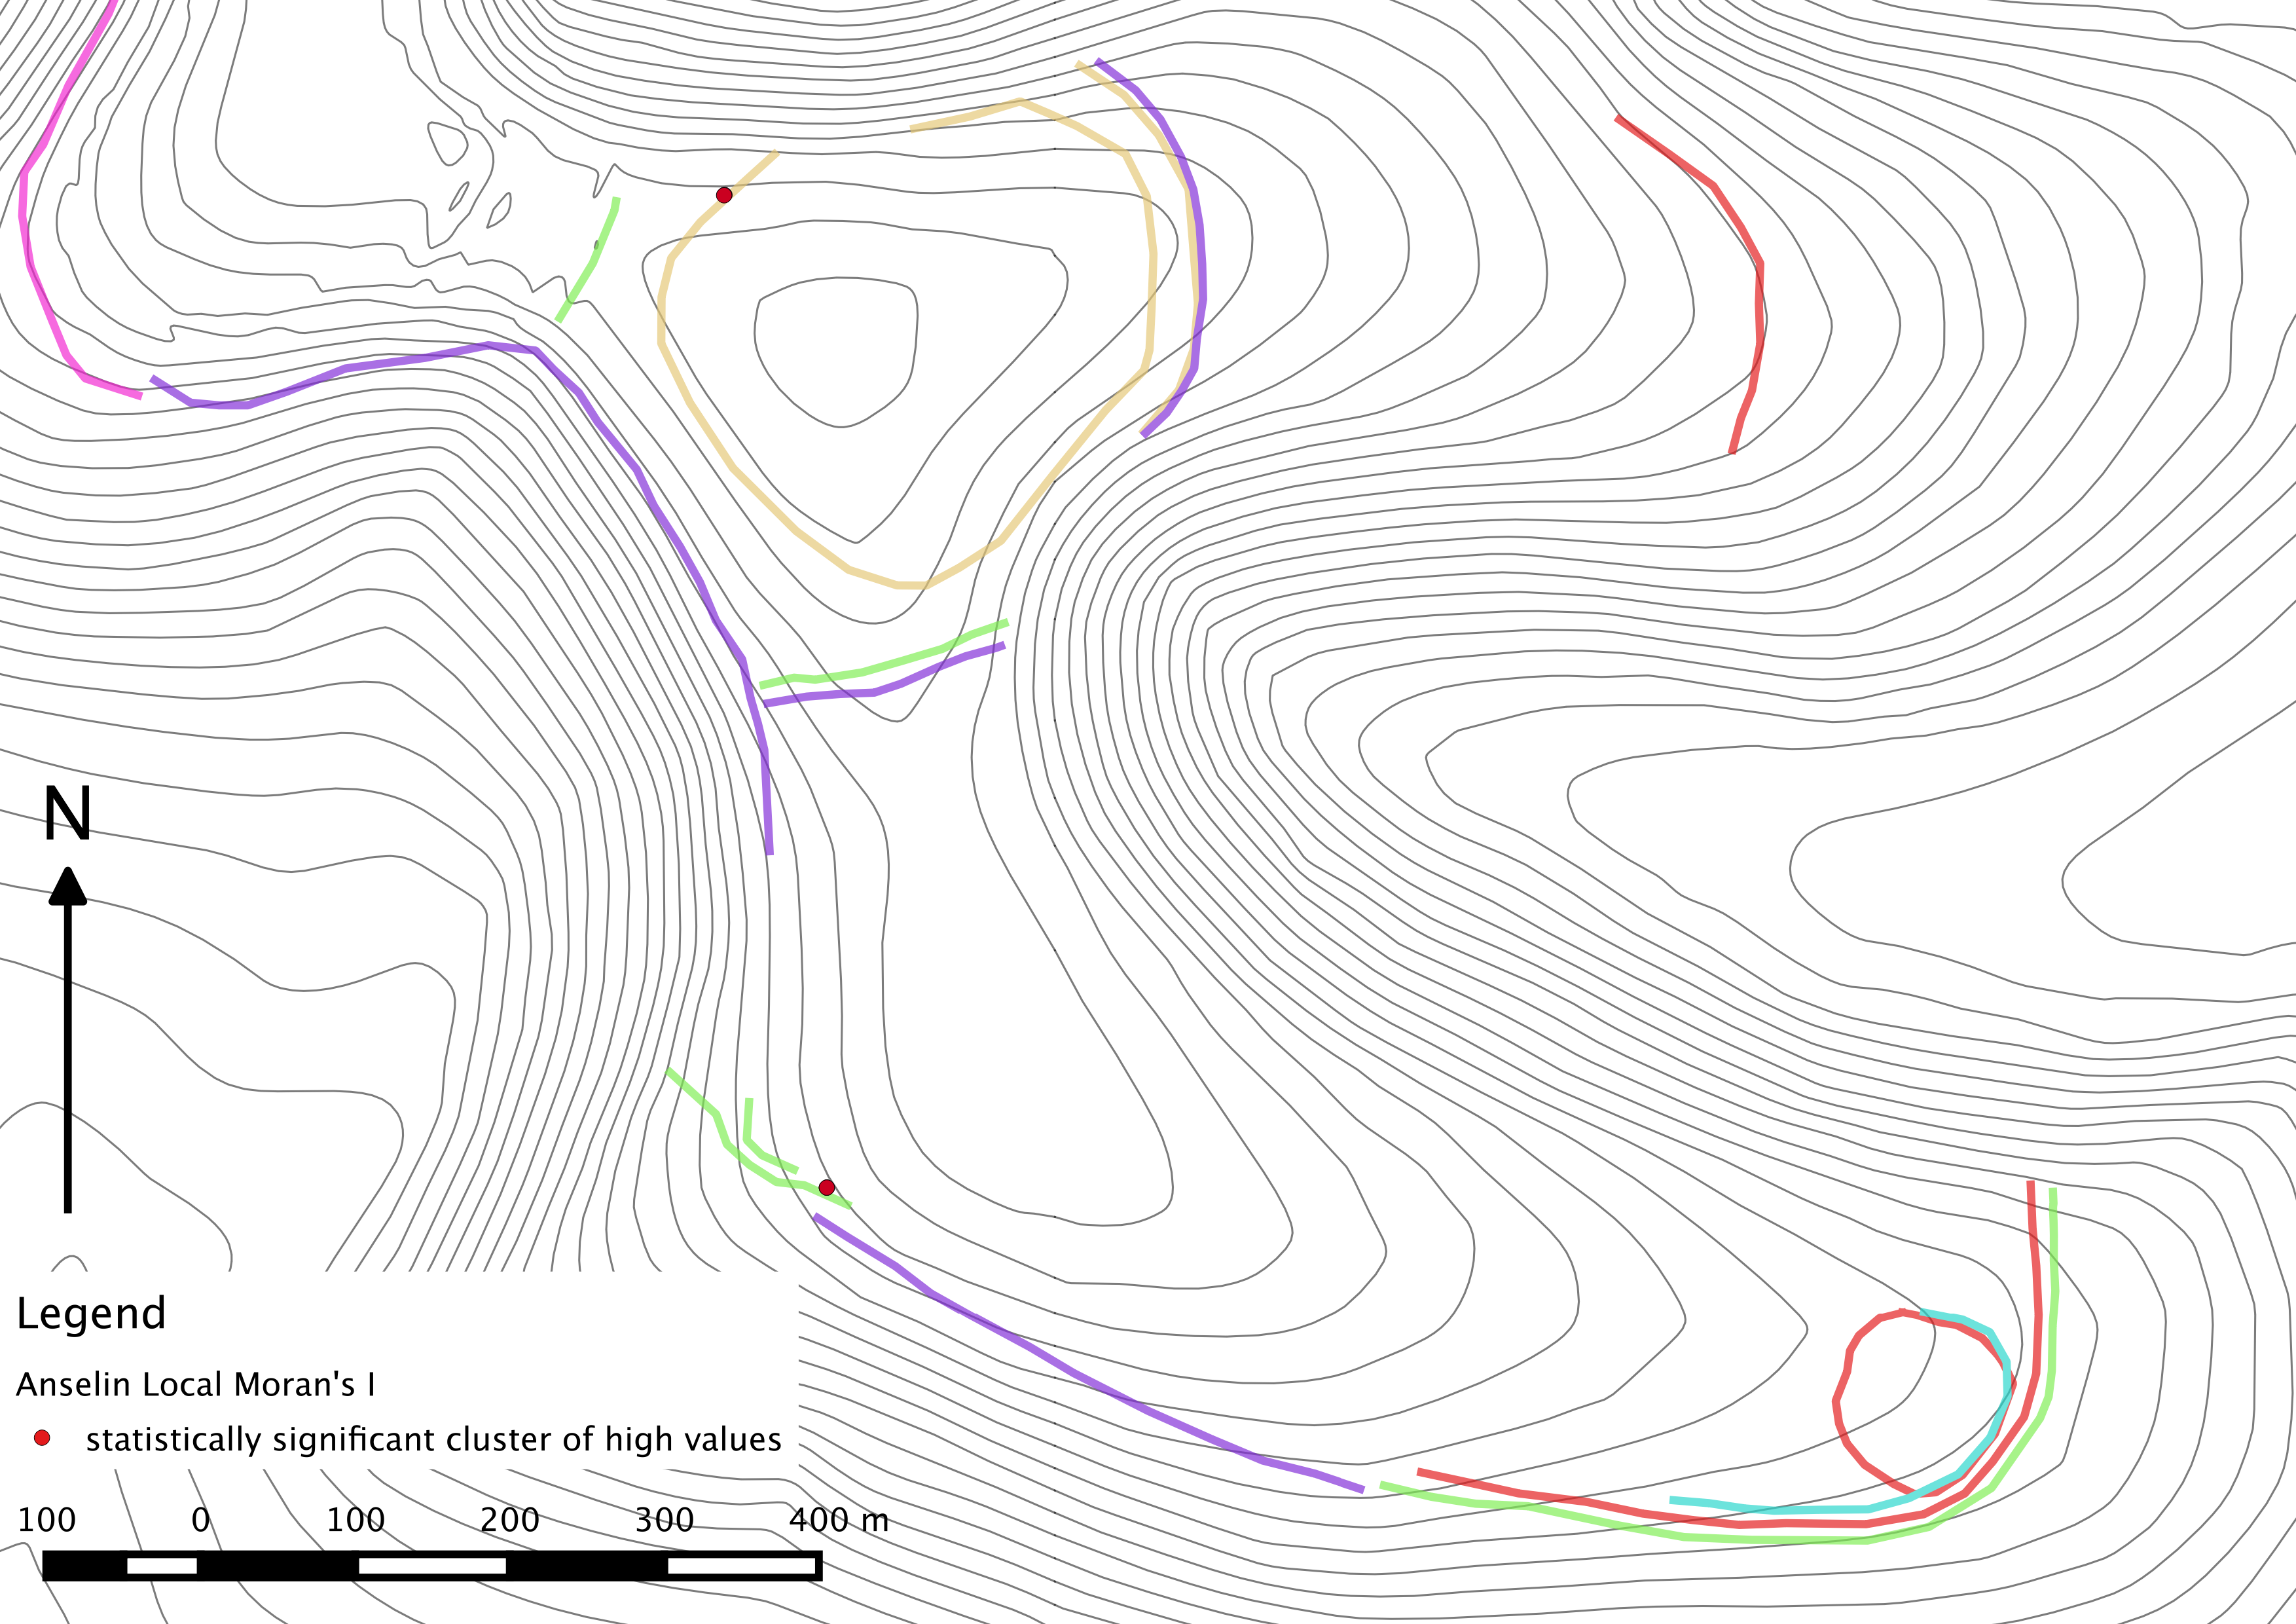
\includegraphics[width=0.8\textwidth]{figures/cluster-HH-mean}
	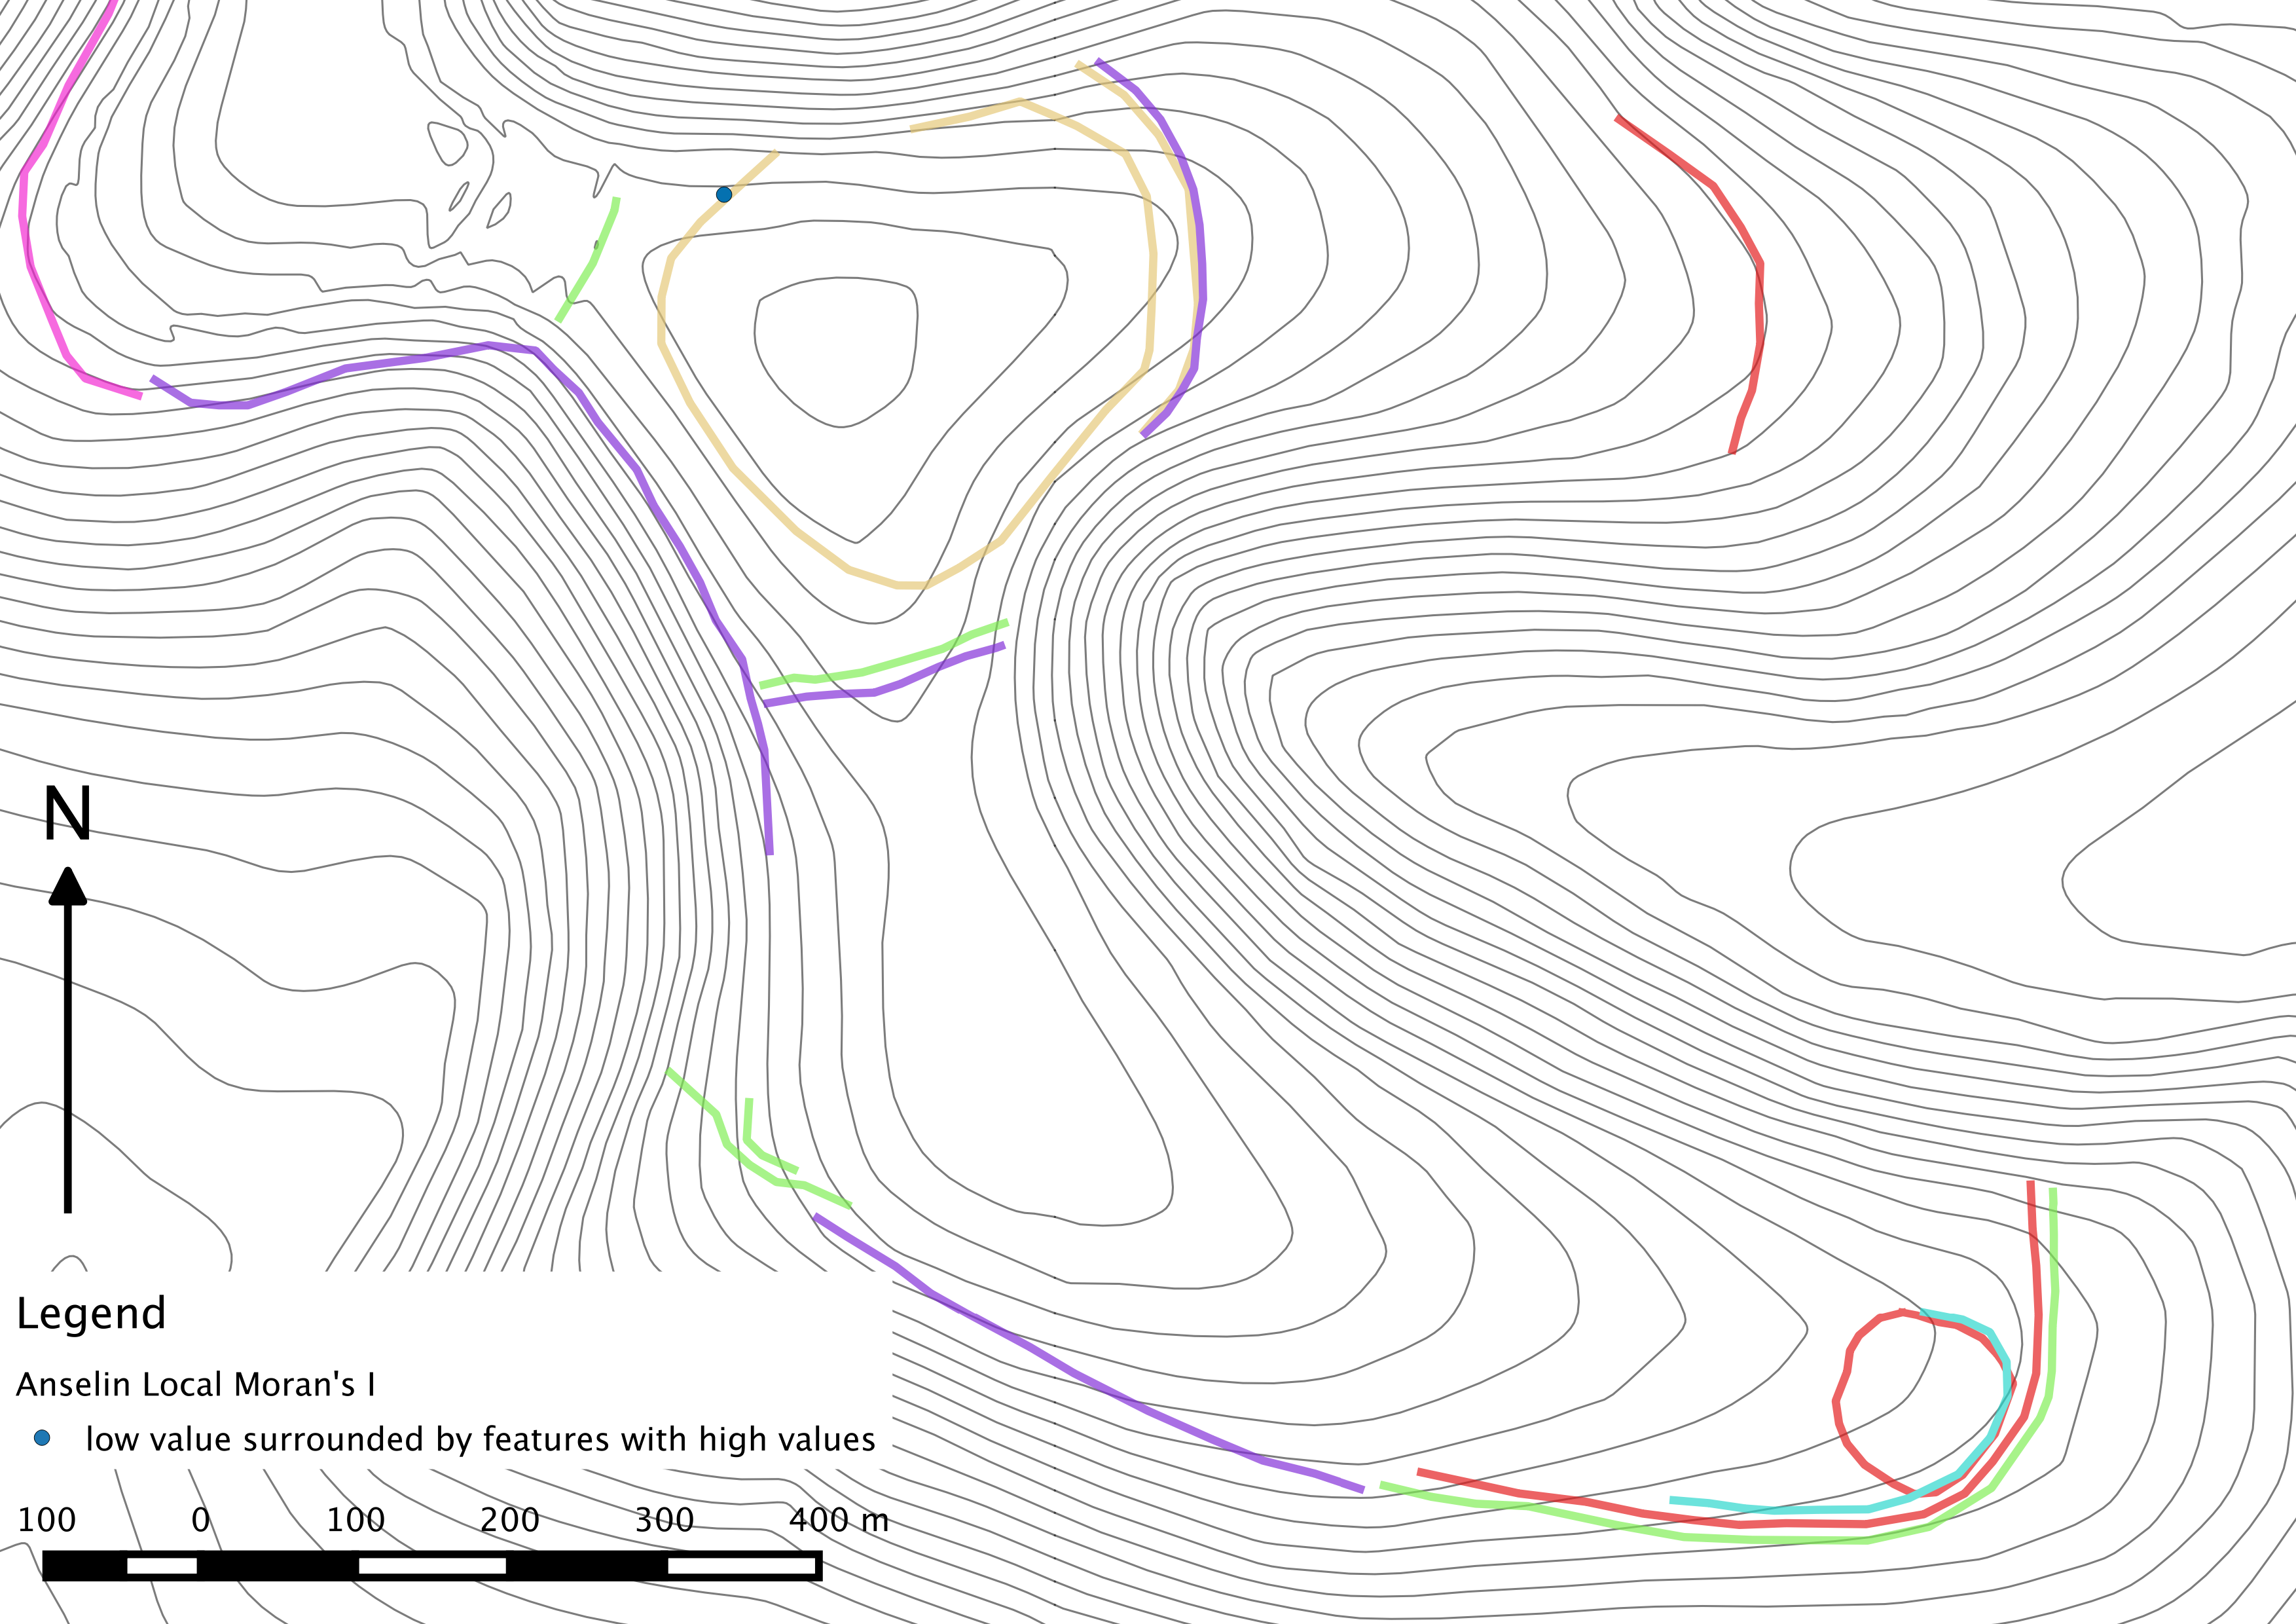
\includegraphics[width=0.8\textwidth]{figures/cluster-LH-mean}
  \caption{Plan of statistically significant clusters and outliers based on a spatial conceptualisation of space}
  \label{fig:cluster-mean}
\end{figure}

As a comparison, figure~\ref{fig:cluster-mean} shows the results of running the Anselin Local Moran's i using the raw spatial locations and their distance as the conceptualisation of space and the mean as the value. This shows the key locations are the same, and analysing the raw results shows that it is in fact the same dates which are identified as clusters and outliers. This suggest the inclusion of chronology and transformation of spatial relationship to a binary value has had little to no effect over the final identification of clusters and outliers. And based on the analysis above, it is clear that the identification of clusters and outliers provides mixed results, some due to facets of the samples and others down to the underlying archaeological data. 

\subsubsection{Getis-Ord Gi*}
Another potentially valuable local statistic is Getis-Ord Gi*, a measure of whether high or low values cluster spatially. The output z-scores shows hot spots and cold spots as large positive and negative z-scores, in this case hot spots are later values surrounded by other later values and cold spots are earlier values surrounded by other earlier values. The values used are the same average value from the posterior density distribution of the bayesian modelled date as used previously.

\begin{figure}
\centering
	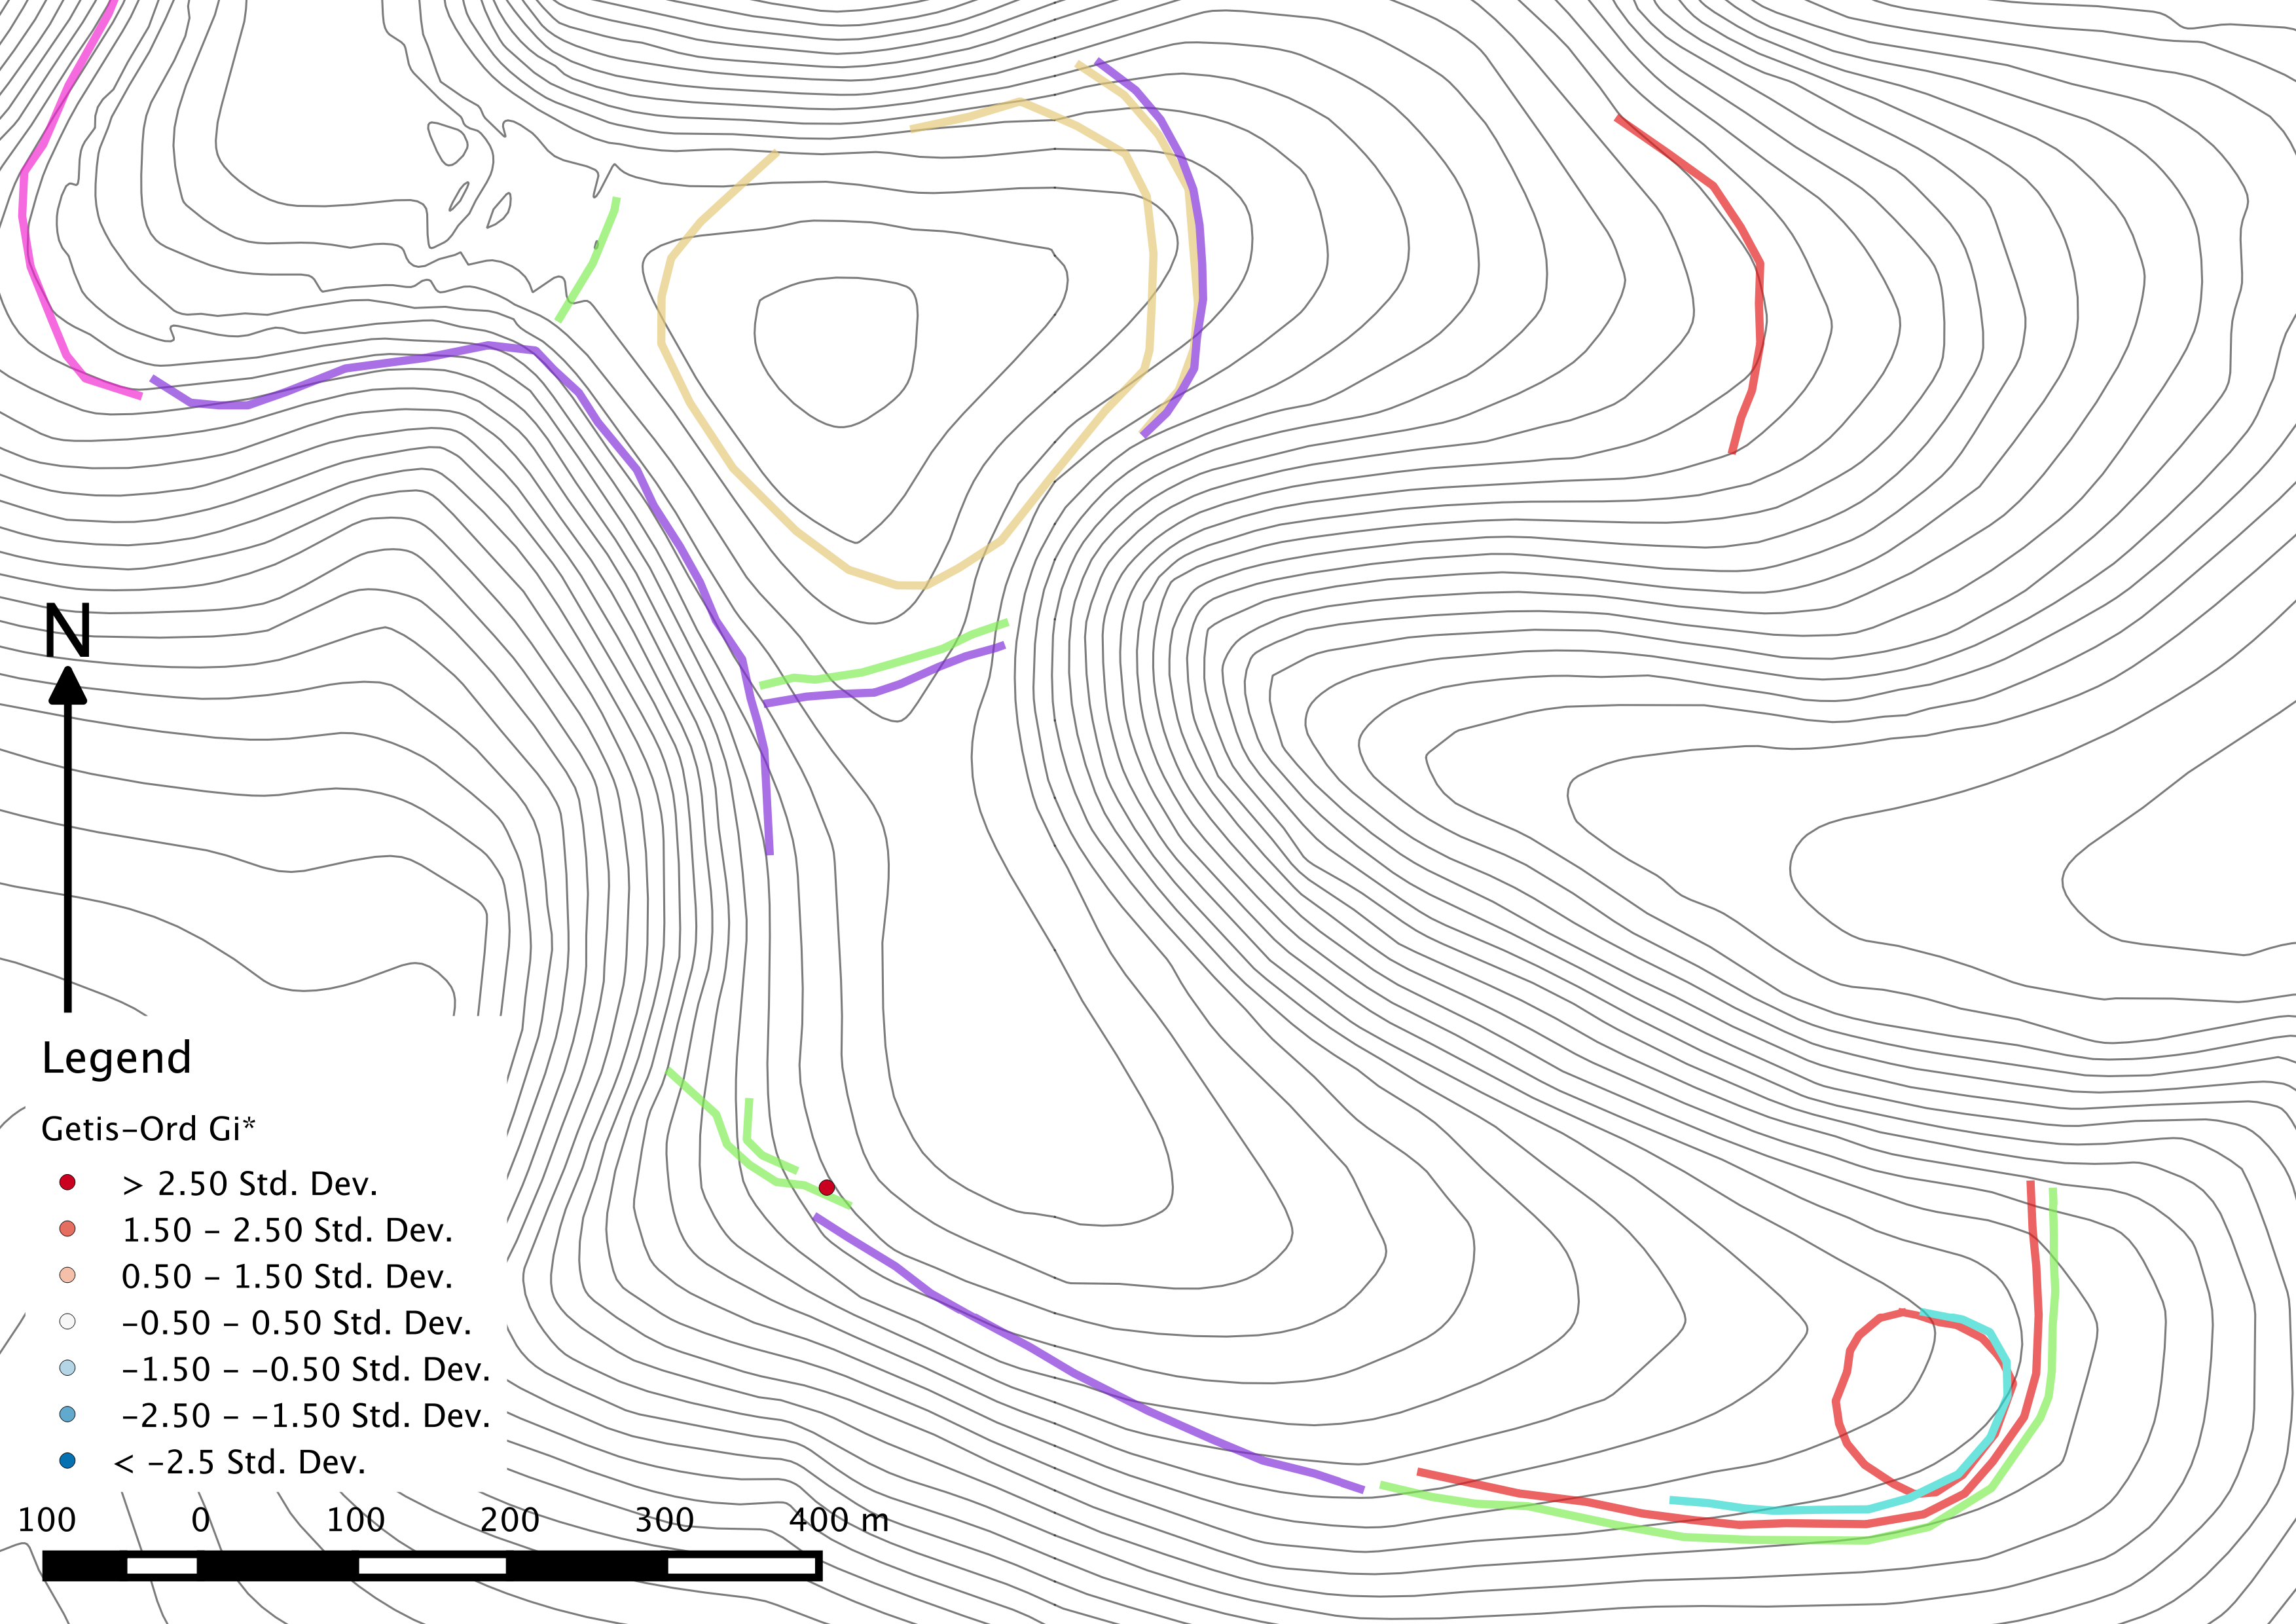
\includegraphics[width=0.8\textwidth]{figures/hotspot-1}
  \caption{Plans of most significant positive z-score values ( $>$ 2.5 Std. Dev.)  for Getis-Ord Gi*}
  \label{fig:hotspot-1}
\end{figure}

\begin{figure}
\centering
	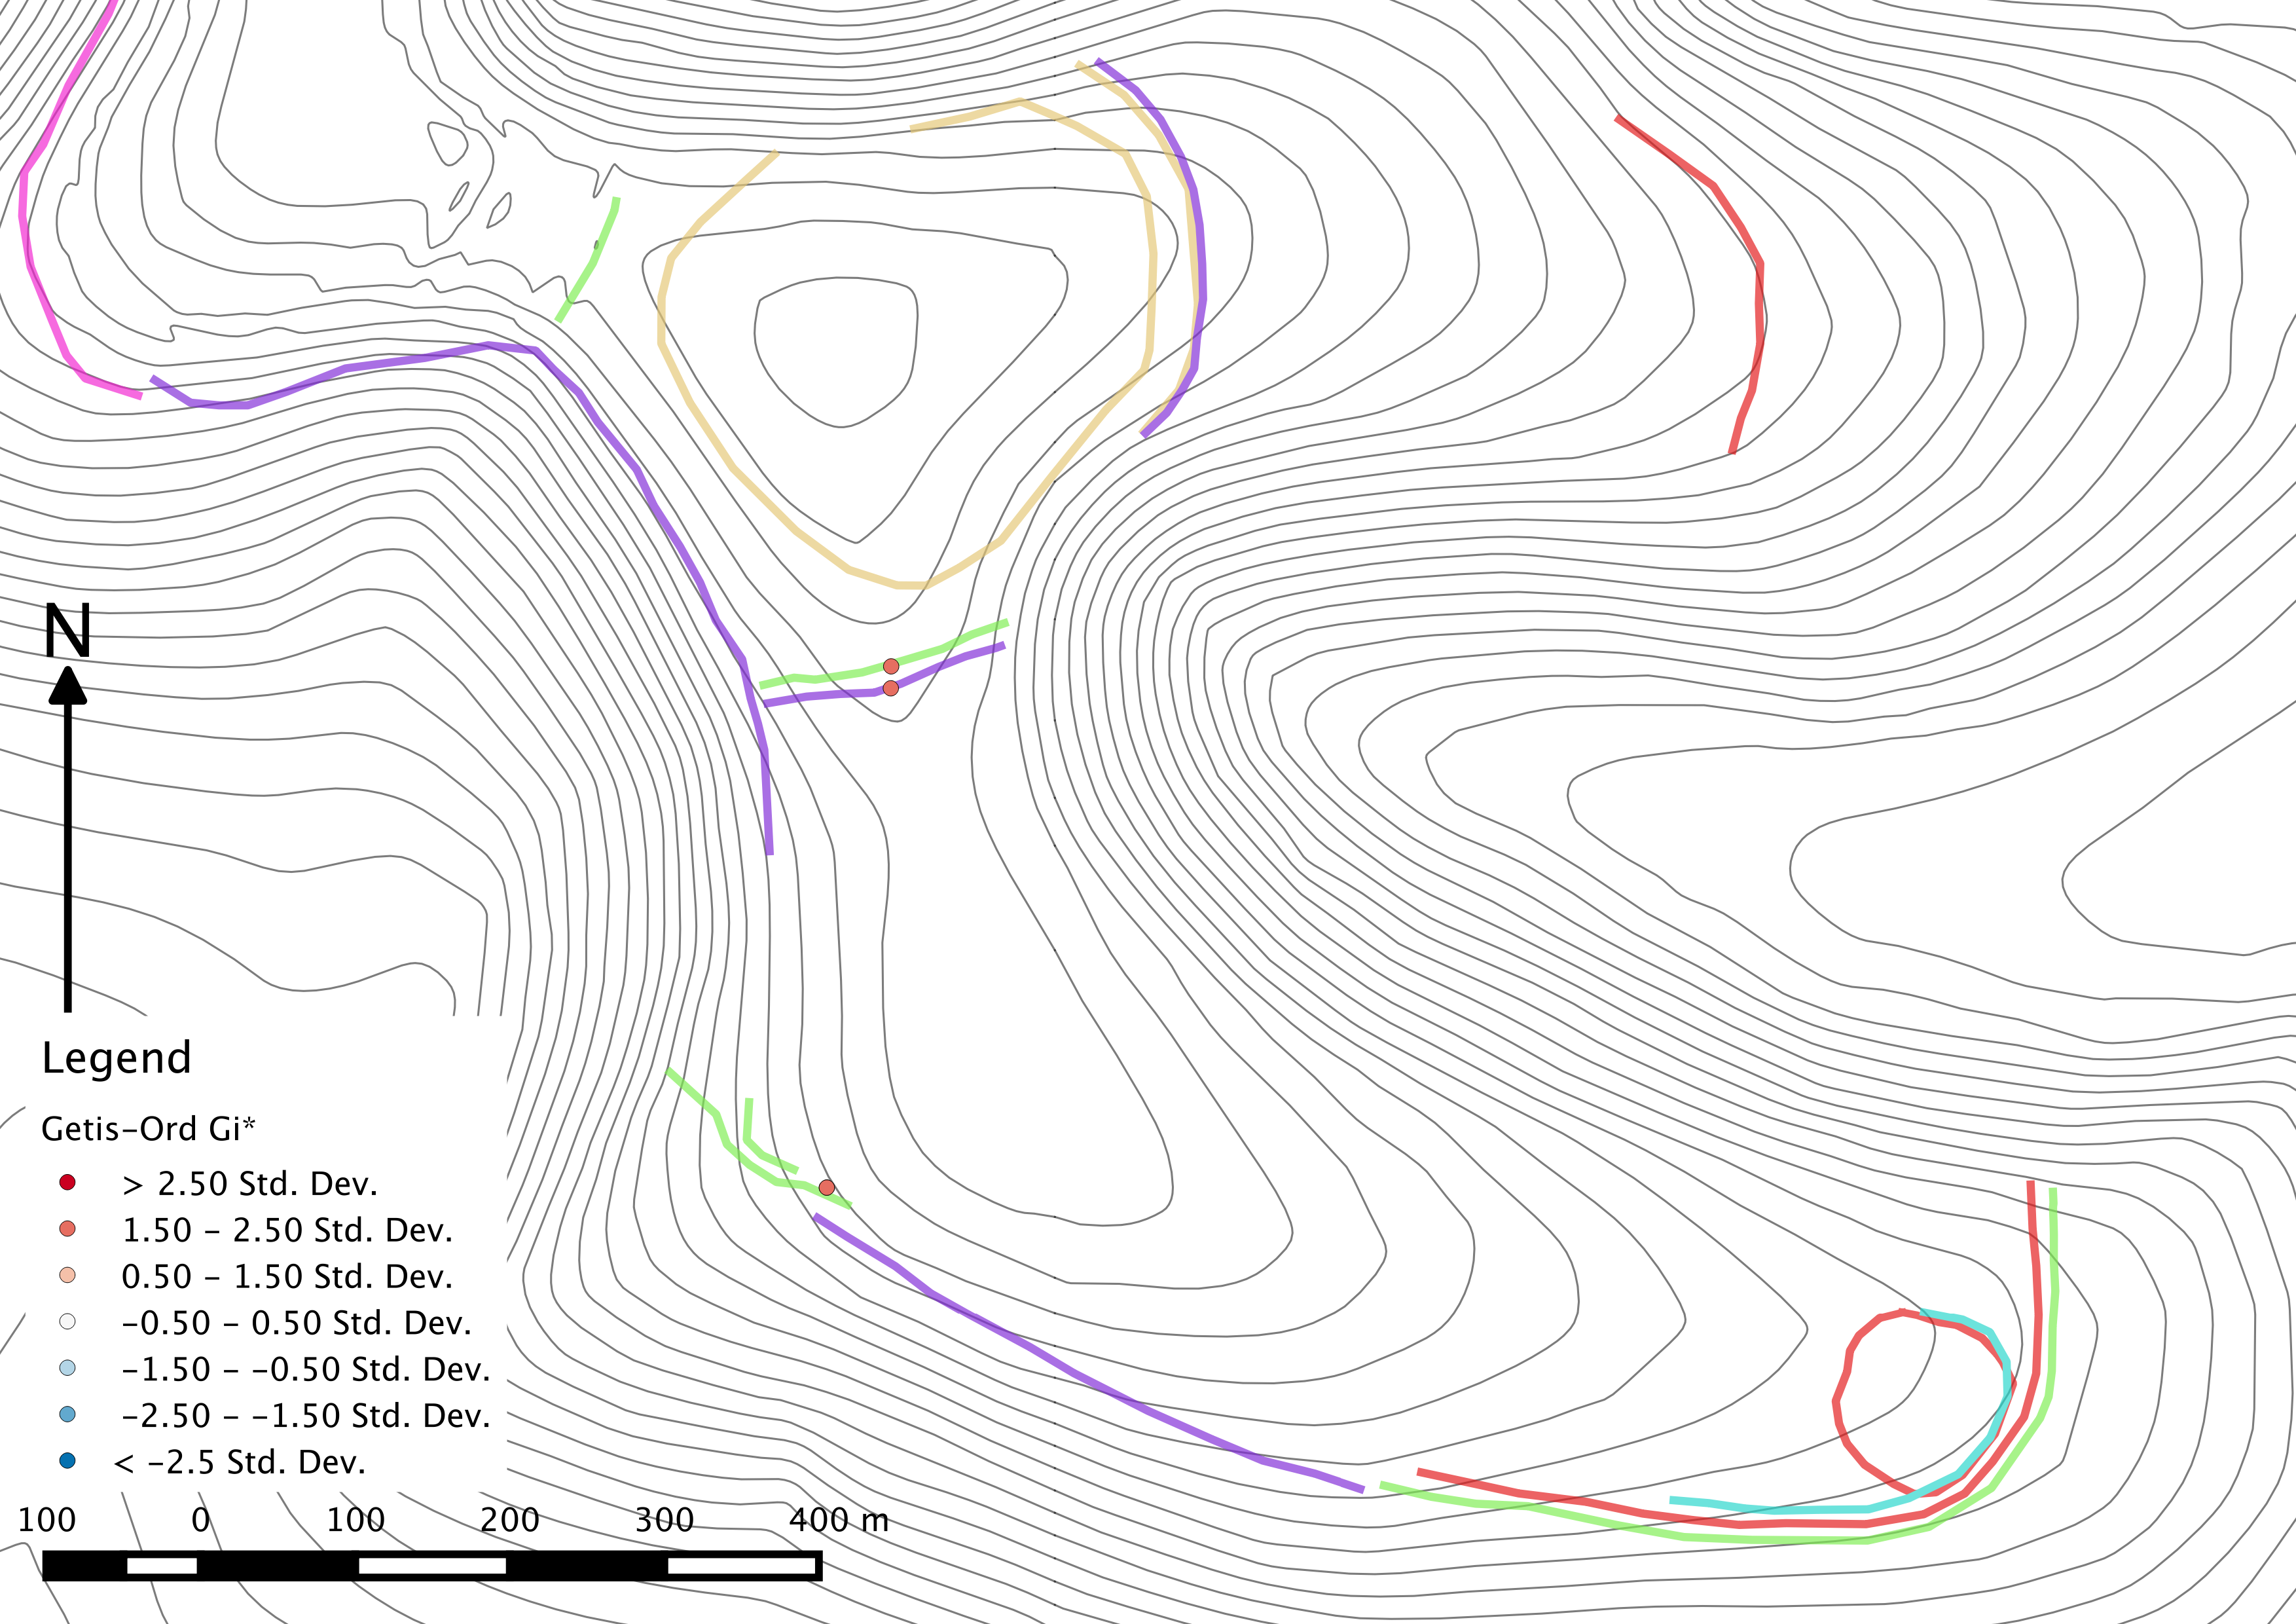
\includegraphics[width=0.8\textwidth]{figures/hotspot-2}
	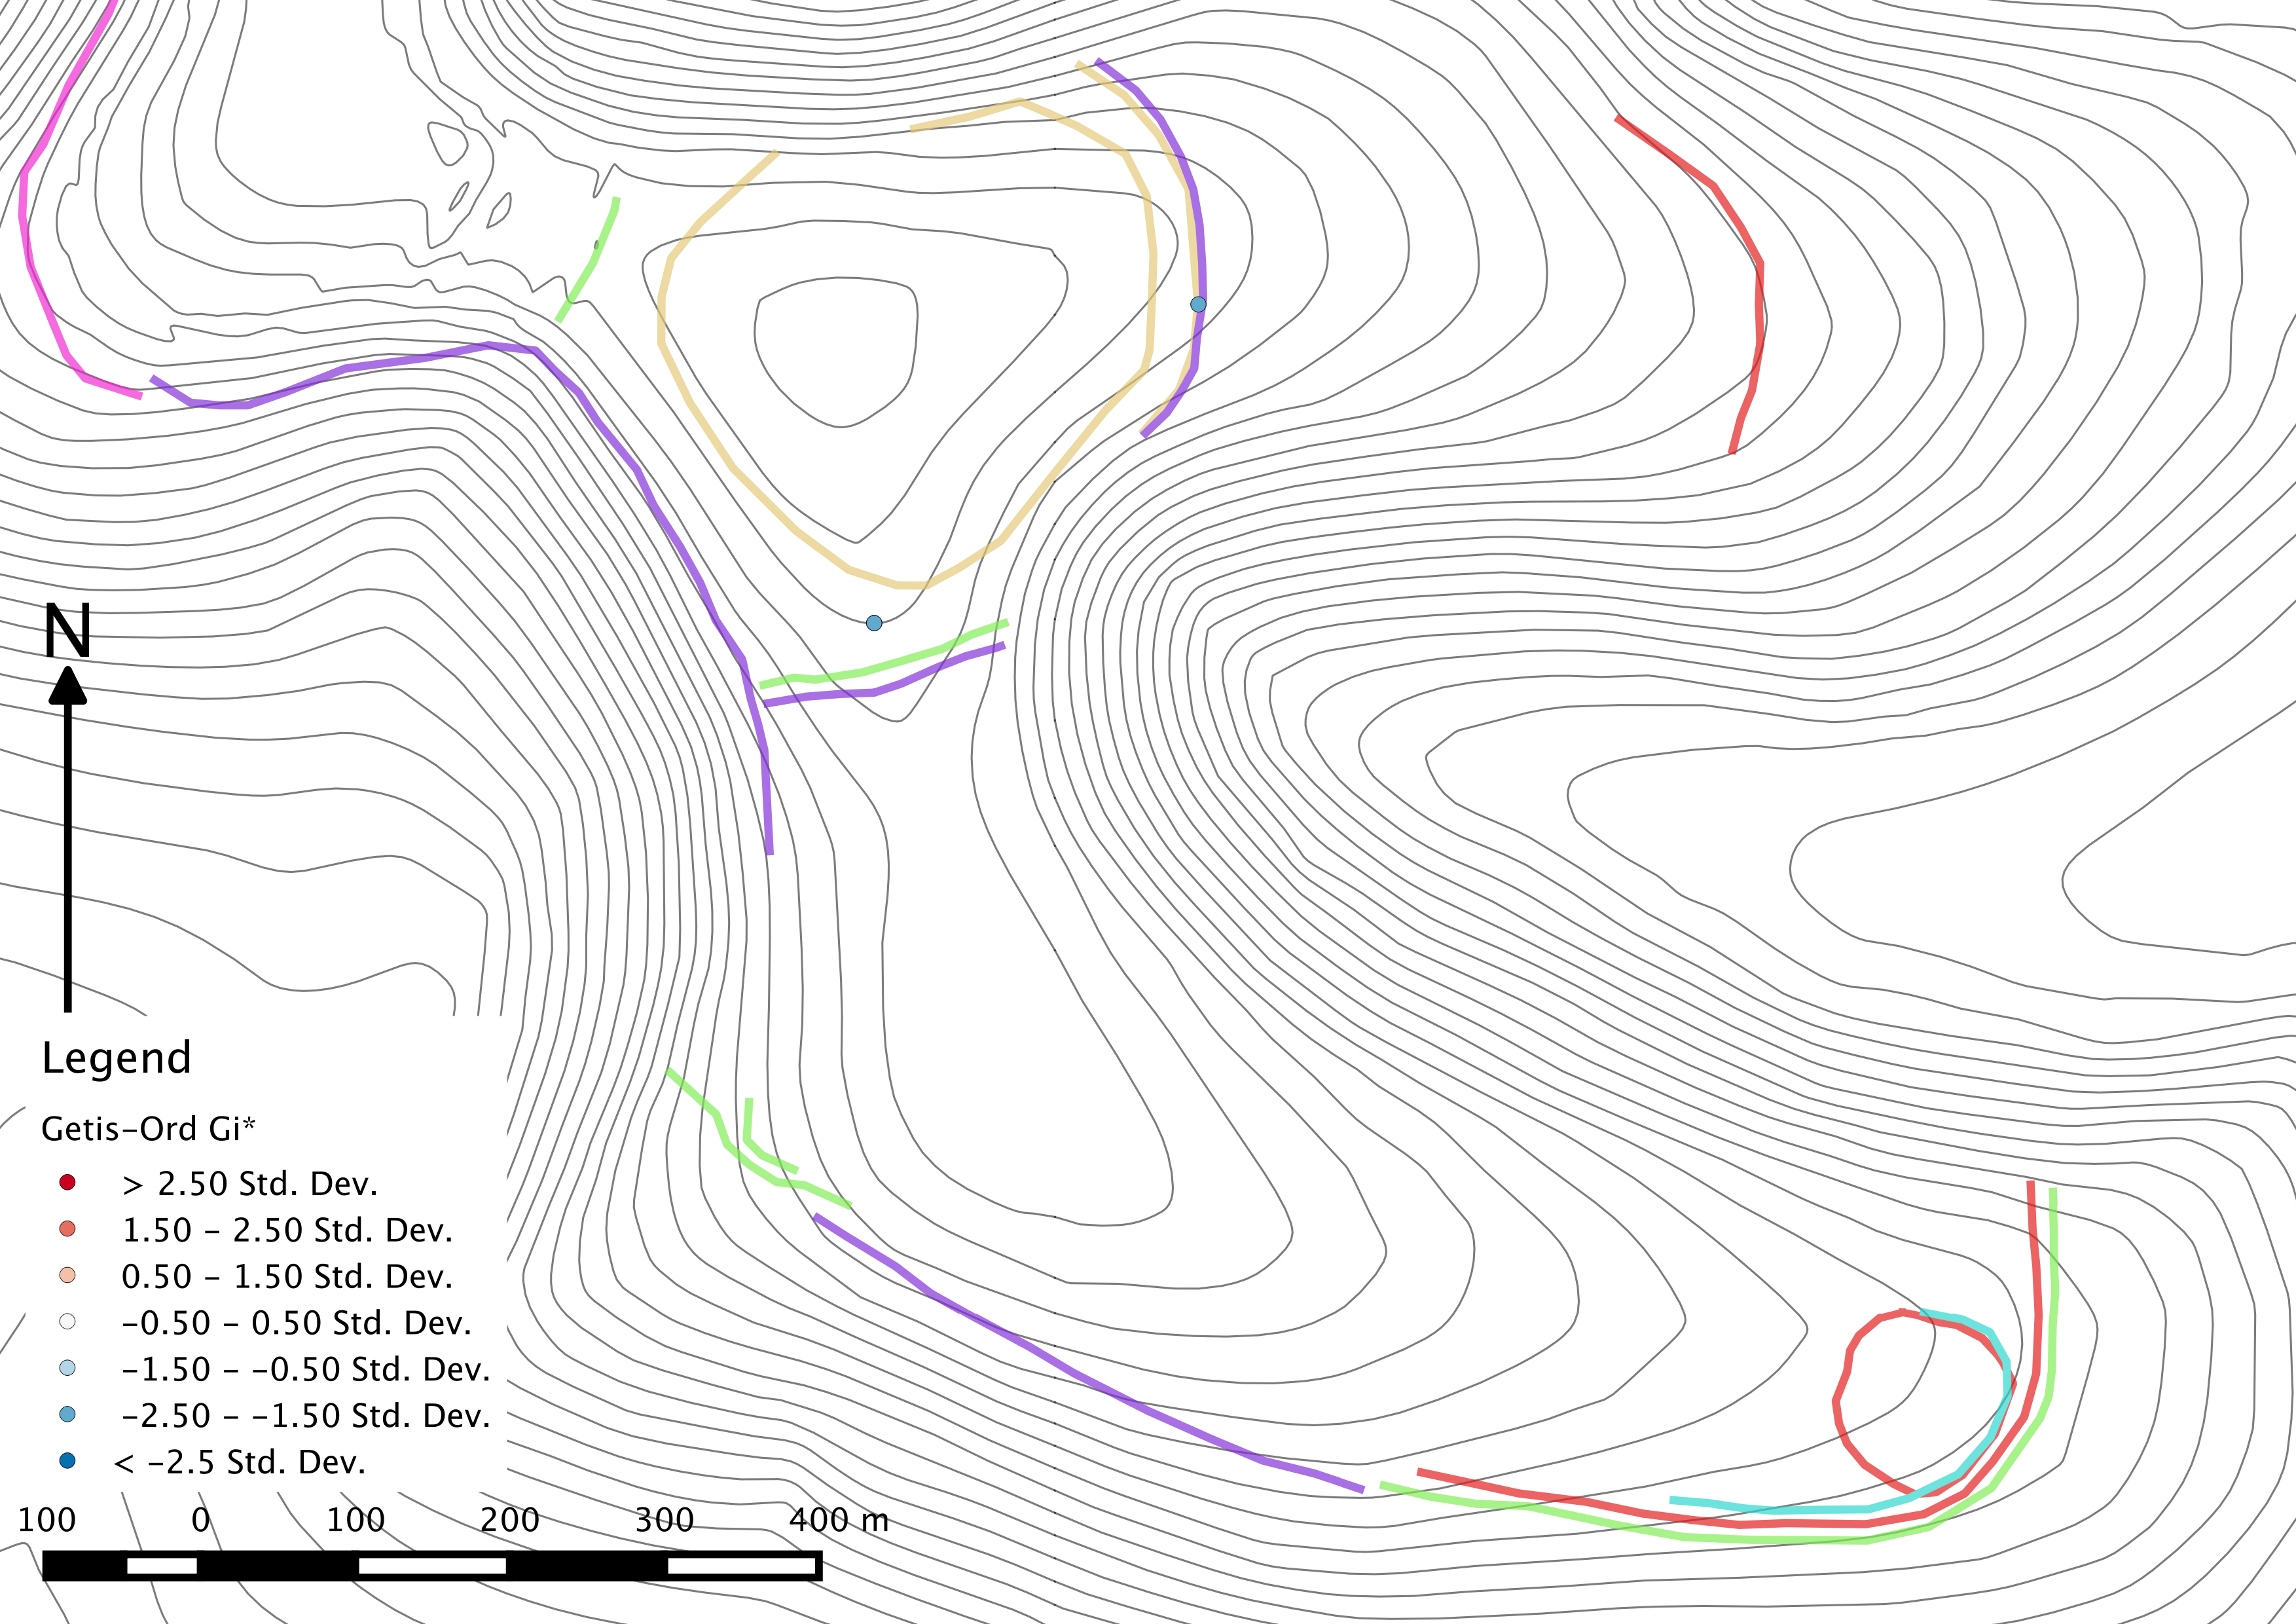
\includegraphics[width=0.8\textwidth]{figures/hotspot-6}
  \caption{Plans of other significant positive and negative z-score values ($>$1.5 and $<$ 2.5 and $<$ -1.5 and $>$ -2.5 Std. Dev.)  for Getis-Ord Gi*}
  \label{fig:hotspot-2}
\end{figure}

\begin{figure}
\centering
	\includegraphics[width=0.7\textwidth]{figures/hotspot-3}
	\includegraphics[width=0.7\textwidth]{figures/hotspot-4}
	\includegraphics[width=0.7\textwidth]{figures/hotspot-5}
  \caption{Plans of least significant positive and negative z-score values (between +1.5 and -1.5 in steps of one Std. Dev.)  for Getis-Ord Gi*}
  \label{fig:hotspot-3}
\end{figure}

Figure~\ref{fig:hotspot-1} shows the most significant hot spots calculated using Getis-Ord Gi*, (there are no correspondingly significant cold spots). There is only one such value, located in the Hanford Outworks, HAR-6038. This was taken from bulked unidentified charcoal, and is modelled as in phase with two other dates UB-4271 and UB-4272 at the same location, there is also date OxA-7850 from the Hanford Outworks. In interpreting this hot spot, it is important to remember that the date values used were averages from the probability distribution (-3424 B.C., -3326  B.C., -3329  B.C. and -3546  B.C.). In this case the distributions of the three dates in phase were very similar, which will have resulted in average values that were also very close together. As there are only four dates from this part of the site included in the bayesian model, a hot spot here indicates this is an area which would benefit from having more samples dated.

Figure~\ref{fig:hotspot-2} shows significant positive, and significant cold spots. There are four such positive hot spots. From the inner south cross dyke is UB-4268 and OxA-7825. This feature also provided sample OxA-7826, respectively they have mean dates of -3553  B.C., -3410  B.C. and -3350  B.C. In this part of the site, there is also the southern long barrow (nine dates, averages from -3638 to -3403), western outworks (OxA-8861, -3576 B.C. and OxA-8862 -3542 B.C.) and segments from the central enclosure (OxA-8851, -3627 B.C.). This hot spot is potentially an identifiable focus of activity, although the particular dates must be treated with the utmost caution as they are averages from the probability distribution. The different features are identified as coming from distinct phases in the chronology, with the main enclosure and long barrow coming from period 1A, the inner south cross dyke from period three and the western outwork from period four. The bayesian model for the inner south cross dyke has two components. From the pre-inner south cross-dyke there are two dates, (OxA-8861 and OxA-8862) which are in fact from the western outwork (and are of Boreal date), but included in this part of the model due to its stratigraphy. And from the recuts phase, date UB-4273 is also actually from the western outwork. This ultimately leaves very few dates from the rest of the inner south cross-dyke, (OxA-7825, OxA-7826, NPL-76, UB-4268) with two coming from the same context (OxA-7825 and OxA-7826) so the close averages for these dates must be a strong factor in its identification as a hotspot. 

UB-4272 and UB-4271 are from the Hanford Outworks, and are related to the hot spot from figure~\ref{fig:hotspot-1}.

Figure~\ref{fig:hotspot-2} also shows three significant cold spots. Two are from the south long barrow (OxA-8847 and OxA-8848 with mean dates of -3596 and -3571). There are ten dates from the south long barrow and an inspection of the model, reproduced in figure~\ref{fig:crossdykes} clearly shows that this particular cold spot is not simply a facet of the averages, but the closeness of the modelled dates is visually apparent as well. These two dates are both from LB2 (the barrow being excavated in quarters) and from phase one in the stratigraphic model, along with OxA-8846 and OxA-7848, which also show the same homogeneity in the underlying probability distribution. Other dates in the model, which are close in space and time, also share a very similar probability distribution, this would combine to create the strong cold spot identified by the algorithm. However, it is crucial to note that four of these dates are in fact from the same layer of primary silt, OxA-7848, OxA-8846, OxaA-8847 and OxA-8848. This may ultimately mean that this particular area has had a disproportionate affect on the algorithm, and draws our attention to an important theme on the nature of archaeological data. This is to what extent can archaeological data be treated as a random sample (for the purposes of performing statistical analysis)? In this case, that data points are not spread randomly through space and time, there being a cluster of such points in the same long barrow ditch, from the same phase. It is perhaps not surprising that such a cluster would be identified as a hot (or cold) spot.

The other is from the inner east cross dyke (OxA-8856 with mean date of -3547). There were a total of six dates from this feature, (OxA-8893 was accidentally omitted from the model, Alex Bayliss, personal communication) of which, OxA-8856 and OxA-8857 belong to the same context in segment four, three belong to another context in segment four and the other is from segment five. The model, figure~\ref{fig:crossdykes}, shows high agreement among the dates, apart from OxA-8857. As before, this cold spot may be an identified locus of activity, or it may be an artefact of the available data. In this case the latter seems likely due to the very limited spatial and temporal spread and the small number of dates in this area.

While both of these cold spots have limited dates in the immediate locality, there are a greater numbers of dates in the wider area and across neighbouring features, which suggests that while the data has clearly had an effect, it may not be quite so clear cut, the cold spots could also be an indicator of an area that was a focus of activity. 

Figure~\ref{fig:hotspot-3} show the remaining date values, with the z-score values split into three groups. These figures includes all other values, so they are not regarded as significant, or worth further investigation based on the z-score alone.

\subsection{The Value of Quantitative Approaches}
These results are not providing earth shattering insights into the lives of past people, but they are descriptive of the data, the same data that has been used to draw insights into the archaeology of Hambledon Hill. The benefits of using such techniques is a more thorough understanding of the data available, which can be used to ensure that any conclusions drawn from that data respect its limitations. 

At Hambledon, the global Moran's i has provided a numeric basis for an observation on the data, that dates within features show positive autocorrelation. Across the site, within features, dates will tend to be chronologically close, rather than evenly spread out. The weighting used here is based on only a 1-dimensional representation of space, which could be improved upon. If the dates were recorded with a more detailed location, this would make that easier - although it would still be necessary to calculate a single weight value from both the spatial distance and the temporal. Without this data it is either a case of calculating a less detailed metric, as above, or creating a false sense of accuracy by assigning co-ordinates to each date. Crucially the global metric is a relatively cheap way of confirming an observation, and informing a route for a more detailed investigation, using local measures.

The Anselin Local Moran's i draws our attention to two areas of the site, one offers a detailed view of a segment of the site's chronology, showing the potential for a detailed interpretation of areas that have a spread of dates through the chronology. And the other, a location where multiple dates on the same samples or contexts made up a large part of the chronology, which could benefit from more dates, spread through the chronology. Clearly the results of this method require detailed investigation as they offer very different opportunities, despite both being represented as clusters around certain date values. The technique enables us to probe parts of the site at both ends of the spectrum in terms of the detail provided by their chronology, while it can offer interpretative opportunities, the technique itself is primarily descriptive of the data set.

The Getis-Ord Gi* analysis was able to identify a number of clusters, several regarded as significant hot or cold spots. In this case, all the areas identified are probably due to there only being a small number of dates in the particular area, that have come from relatively close parts of the chronology and so have close enough average values to be identified as a hot (or cold) spot.
The Hanford outworks, which was also identified by the Local Moran's i, is identified twice by the Getis-Ord Gi* analysis, it is clearly an area of the site that would benefit considerably from more investigation, ideally leading to more dates distributed through its chronology. The re-analysis of section 17, above, demonstrates the added value of this, where a single date (or where only a single context or phase is dated) simply provides a point in time, where as successive dates enable a discussion around duration, a consideration of the passage of time, how the site changed and was modified and across what length of time. Crucially, a series of dates enables the bayesian statistical method to work most effectively and remove some uncertainty (with certain modelled assumptions) from the date values.

Also identified by the Getis-Ord Gi* analysis is a hot spot at the inner south cross dyke, however a detailed analysis of the data reveals that, again this is an area with very few dates, with limited spread through the chronology. As with the Hanford outwork, what has been identified here is an area of limited temporal evidence, where any detailed interpretation should be treated with the utmost caution. In addition to this there are two distinct areas of cold spots, one at the south long barrow, and the other at the inner east cross dyke. The south long barrow could potentially be either a cluster of activity, or a facet of the data, there are a large number of dates, which span the chronology of the feature (ten dates across five phases) however, half of the dates come from a single phase, phase I and in fact four are from the primary fill. The other dates, (of which two are from the same sample) come from later phases and are dated to much later, potentially in the region of 150 years later or so. This would in fact suggest that the cold spot in this case is down to the dates in the model not being evenly spread through the chronology, but concentrated (or clustered) in the very first part of the feature's life, the primary fills. This demonstrates that while the number of dates is clearly important, it is much more valuable to have the dates spread through the chronology.

The other cold spot, the inner east cross dyke, has as much spatial breadth as temporal in the available data. Three separate contexts were dated, across two segments, and the two dates from segment four both came from the same layer in the primary sit. As does the date from segment five. Chronologically this is in many regards one dimensional, as there is little scope for detailed interpretation when the dates all come from the same part of the features life, even if there are multiple dates spread spatially. It does permit a limited comparison of the two segments, but this would have to be treated with caution, as there is so little dating evidence available.

The methods evaluated above demonstrate the value of performing combined spatio-temporal analysis. Mathematically they can be performed relatively cheaply if a single value proxy to the true probability distribution of the radiocarbon dates is used, but this must be kept in mind when examining results. While there are mathematical ways of performing cluster analysis on probability distributions, with which it might be possible to perform these analysis on the raw data, it is unlikely that the results will be more valuable, and depending on the precise method of cluster analysis, might in fact make interpretation more difficult. The identification of spatio-temporal autocorrelation is an important characteristic of the data set, and it must be kept in mind that this could potentially be the result of a range of different processes. It is possible that any auto-correlation is a result of how the archaeological deposits were laid down, and offers evidence directly pertinent to the interpretation of the site. It may also be due to taphonomic processes, or the structure of the archaeological work or the decisions over what was dated. It is also likely to be influenced by all of these factors. Crucially, the results of any such analysis must be accompanied by a full consideration of the evidence in order to determine the likely cause of the autocorrelation, and any effect this might have on subsequent interpretation. The same is true of the local measures, while they identify specific parts of the site, the same thorough examination of evidence is required in order to determine why they have been identified, and following this it is possible to evaluate an areas impact on any subsequent interpretation of the site. In this chapter the thorough examination of the evidence came first, with a detailed review of the chronology at Hambledon Hill, having performed these statistical tests we can now re-examine the original interpretation with a more thorough understanding of the spatio-temporal nature and limitations of the data set.

\section{Chronology Revisited} 
The focus of both the original report \citep{Mercer:2008fk} and later review \citet{Whittle:2011kl} is on determining start dates, durations of use, length of time between construction of features. While these are important questions, they rely as outlined above, on some assumptions about interpolating the available data. This also does not necessarily give the opportunity for a detailed account of those areas that are relatively well dated, and can provide more than simple date, duration and position in the overall sequence. 

There is little evidence for the earliest, Mesolithic use of the site, several potential large post settings, similar to those at Stonehenge \citep[48]{Mercer:2008fk}, a smaller post setting, and several episodes of burning, mostly concentrated around the Hanford spur. F279, a large post setting, dated to over 7000 cal BC (OxA-7845 and OxA-7846).

Prior to the construction of the enclosure, there is evidence for Neolithic activity on the hill, with Neolithic artefacts, animal bone and charcoal on the old land surface and in natural features beneath the main enclosure bank \citep[138]{Whittle:2011kl}. This early activity appear to be very small in scale, with the deposits containing small quantities of bowl pottery, struck flint and animal bone \citep[54]{Mercer:2008fk}. However it shows a Neolithic familiarity with the site, and suggests it was a known location for those who built the main enclosure. None of the little material there is from this phase of use has been dated, although those beneath the main enclosure bank must pre-date its construction, in the mid-37th century cal BC. This would suggest that such activity would be at most a few hundred years prior to the construction of the enclosure. Without dates, this is purely speculation, and the material may well come from multiple episodes of activity, over a period of time.

\subsection{Period 1A}
\subsubsection{The Central Area}
Following the general chronology laid down by \citet[136]{Whittle:2011kl} the first period of (monumental) use saw the construction of the main enclosure, inner east cross-dyke and south long barrow, possibly at the same time, certainly with no clear sequence \citep[136]{Whittle:2011kl}. The main enclosure evidence, from eight ditch segments, suggests that they may have been constructed around the same time, however figure~\ref{fig:central-phasei-model} shows that this is not certain. Of course there is also the definition of what is meant by at the same time, even segments five to seven, with the smallest probability around the date of construction still have a time window of around 50 years, the others larger, so it is difficult to asses how close together their construction was. Also this enclosure was estimated to have potentially taken over 7000 worker days \citep[752]{Mercer:2008fk} so it is quite possible that the enclsoure took several years to build.  Such a length of construction time would still easily fit into the probabilities for the construction of the dated ditch segments. Segments five, six and seven mostly have dates from the primary silt, phase I, combined, the start of construction in the bayesian model is dated to 3686-3620 cal BC (90.9\%) or 3604-3574 cal BC (4.8\%). While this is useful answering questions on the start of construction, and relative dates of construction between features, dates spread throughout the chronology would enable a more detailed examination. There is also HH76 2625, two replicated dates from the lower trunk and femurs of a young male, cut marked and dog gnawed \citep[119]{Whittle:2011kl} placed on the surface of the phase II silts in segment six, dated to 3455-3375 cal B.C. Compared to the phase I dates for segment six, OxA-8852 3620-3610 cal B.C. (1\%) or 3520-3405 (94\%) and OxA-8853, 3655-3505 (93\%) or 3425-3405 (2\%) it is clearly at least 50 years later, possibly as much as 200 years later. The ditch into which these remains were placed had started to silt up, with the phase I and II silts, but was still probably clearly identifiable, atop the human remains was a spread of flint nodules, and chalk blocks \citep[72]{Mercer:2008fk}. By focusing here on the detail surrounding the dates (rather than looking for broad answers about start dates and durations) it is possible to determine, that in segment six at least, the ditch had gone from being regularly maintained and cleaned, as a ditch, to a significant location. Clearly one with a very different meaning and purpose, as rather than being cleaned out, people were being placed into it. The bones being dog gnawed (assuming it happened prior to burial) suggest the corpse was first placed somewhere before being buried here, although as the bones are articulated, presumably he was still buried as a body (or part body) rather than a collection of bones, recognisably human and very likely a known individual.

Segment nine contains a broader spread of dates, from phase I through to end of phase III. The two dates from phase I give this phase a date of 3661-3529 cal B.C. (95.4\%). The two phase II silts are described as grey and powdery, and the original report suggests they appear to have been tipped from the causeway and covered before any of the fine component could be washed away. The dates from these silts have broad probabilities, most being in the region of around 250 years or more (OxA-7027, OxA-7824, HAR-1886, OxA-7028) although OxA-7029 is a bit more limited at 3768-3637 cal B.C. (95.4\%) \citep[81]{Mercer:2008fk}. This would suggest that the primary silts accumulated relatively quickly, and as with segment six there is a clear shift in mindset from cleaning, to dumping, after a fairly short space of time. Although, as these dates are modelled as TPQ it is possible some time could have elapsed before the dated material was placed. The phase III deposits, generally chalk and flint rubble provided a date of 3457-3366 cal B.C. (95.4\%) this is clearly much later than the earlier fills, at least 70 years, possibly more. The source of these fills is attributed to the sides of the ditch and bank \citep[56]{Mercer:2008fk} which would suggest that any structure retaining the bank had by now started to decay. In this segment is a dated sequence from close to the original construction of the ditch, through its maintenance and initial silting, to the manual fills of phase II and what appears to be abandonment of the maintenance of the bank and ditch by phase III, by the end of this phase the ditch would have been a much shallower feature, all taking place over possible maximum of around 300 years, potentially as few 72. 

Segment 16 only provides a single date for the model, OxA-7767, from the primary fills. Segment 18 provides three dates, two being replicates on the same sample, HH76 1948, from the primary fills (3654-3547 cal BC 95.4\% prob) and UB-4269 (3370-3329 cal BC 95.4\%) from phase III. This is modelled as coming from a re-cut, as otherwise the model shows poor agreement for this section, and re-cuts from this phase were potentially missed during excavation \citep[399]{Mercer:2008fk}. However, there is also the possibility that the sequences combined into one for the model, from segments 16-19, are in fact not contemporary, combining non-contemporary dates for a phase would also lead to the poor agreement value. If we assume the model is correct, segment 18 provides a duration from the initial fills of the cutting of the ditch, to a time when the ditch was no more than a shallow depression, into which slots were dug, and material placed (in this case the material included an articulating cattle tibia) in a time period of at least 177 years, potentially as many as 267 years. If the model is not accurate and UB-4269 is from earlier in the chronology (phase III) then these date ranges reflect the time from initial fills of ditch to it being filled by the contents, potentially of the bank and sides, a period of a lack of maintenance.

The relatively well dated chronology of segment 17 has already been noted, in particular the short span of time covered by the dates. To review, three samples were dated from the same context in phase III, four samples from a context in phase IV, two samples from a context in phase VI and a sample dated from a burial post phase VI. The potentially earliest date, from phase III is combined OxA-7022 and OxA-7023 (replicates from sample HH76 2808, dated to 3610-3517 cal BC 95.4\% prob) and the latest, from post VI OxA-7039 and OxA-7040 (replicates from sample HH76 3046, dated to 3374-3319 cal BC 95.4\% prob) have a duration between the two of between 291 and 143 years. The phase III fills, being the bulk of the fills would have started to accumulate into a only slightly denuded ditch, which by the end the chronology for segment 17 was little more than a ``shallow depression'' \cite[56]{Mercer:2008fk}. It provides a well dated sequence for the later part of the Neolithic use life of the ditch, after it had ceased to serve as a physical boundary. A life consisting of material deliberately being placed in the ditch, starting with the dump of ashy material in phase IV, then the digging of slots and potentially placement of containers of various material in phase VI, which are subsequently covered by flint cairns, and finally the burial, cut into the side of the causeway. While the ditch may no longer have served as a physical boundary, it is clearly still a recognised feature in the landscape, subject to distinct treatment, perhaps still a liminal boundary. The successively different behaviours could indicate different successive phases of use, possibly re-interpretation of the site, by subsequent generations, possibly with a hiatus in between. Although the last point is unfortunately only conjecture, as neither the dating evidence of stratigraphy provides enough information to support such conclusions.

Segment 19 provided two dates on samples from the same context, in either phase I or phase III. They are modelled in phase III as a TPQ, and provide in this case, little more than a date before which the bulk of the fill accumulated in this segment.

To summarise for the central enclosure then, there is clear evidence that three segments were dug by 3687-3636 cal BC (build main enclosure first, 95.4\% prob). The ditches were kept clear for a time, but in some segments the phase II deposits were dumped into the ditch. Phase III perhaps marks the decay of any structure retaining the bank, this possibly coincides with less activity in this part of the site, as the ditches fill up with rubble. This would suggest that the enclosure remained in its original form for perhaps 100 years or so. However even if there were periods (perhaps prolonged) of abandonments, people continue to use the main enclosure, specifically the ditches, for placing a series of deposits, including other people. This brief summary draws on evidence from across the site, as the bayesian model does, however the different phases did take different forms between segments, and while we can compare the chronology for all segments, we cannot compare dates where we do not have any, so any broad summary must be appropriately vague.

\subsubsection{Cross Dykes and the Long Barrow}
The east cross-dykes provided relatively few dates, all those included in the model for the inner east cross-dyke are from phase I, and are statistically significantly different \citep[401]{Mercer:2008fk}. There is only a single date from the outer east cross-dyke, also from phase I. The dating evidence provides little additional detail on top of a broad date for the initial building of the inner east cross-dyke of 3686-3644 cal BC (95.4\% prob). 

The south long barrow has already been discussed, it had a great disparity in the spread of the dates, with half coming from the primary silts of the ditches, providing a good amount of evidence for the building of the long barrow of 3687-3643 cal BC (95.4\% prob). Subsequent dates from the ditches provide evidence for their respective fills. There are no dates in the model from the barrow mound or its contents, so from a chronology perspective it is only possible place its construction within the context of the whole site.

\subsection{Period 1B}
\subsubsection{The Shroton Spur Outworks}
The second period in the sites chronology is period 1B, into which \citet{Whittle:2011kl} have placed the Shroton spur outwork, Stepleton enclosure and middle Stepleton outwork. The Shroton spur outworks are sparsely dated, there is clear evidence from the initial fills dating the construction (dates from antler picks found on the ditch bottom) to around 3640-3576 cal BC (95.4\% prob) and then dates from phase III, of the main fills, which silted naturally \citep[189]{Mercer:2008fk}. The dates from this phase have a fairly broad spread, for example OxA-7832, 3516-3346 cal BC (95.4\% prob) clearly later than the phase I fills, potentially anything from a few decades, to around 200 years, with the gradual nature of the fills suggesting a longer duration is more likely. The broad nature of these dates makes comparison with the central enclosure tricky, but the date ranges clearly start later for both the initial, and main fills. With the main fill date ranges being later than most of those for phase II and phase III fills for the central enclosure.

\subsubsection{The Stepleton Enclosure}
The Stepleton enclosure is dated by several segments, segment three has five dates from phase I, which provide the date for the building of the outwork at 3641-3574 cal BC (95.4\% prob) and five from phase IV, there is also one date from segment ten and two on the same context from segment seven. The dates from segment three bracket the main fills of the ditch, however the probabilities are particularly large, e.g. OxA-7050 is 3575-3485 cal BC (47\%) or 3470-3380 cal BC (48\%) making it difficult to draw any detailed conclusions from the dates. Compared to the main enclosure, the latter of these two ranges is similar to the date probabilities for those from phase III, so the filling in of the ditches at the Stepleton enclosure might have been happening at the same time. The dates for the middle Stepleton outwork suffer from the same absence of evidence, of three segments dated, only segment six has had more than one context dated. Segment six has three dates from the ditch base, which give a date of initial construction of 3640-3591 cal BC (95.4\% prob) and UB-4136 from phase III dated to 3495-3465 cal BC (27\% prob) 3380-3340 cal BC (68\% prob). As with the Stepleton enclosure, these dates bracket the fill of a single ditch, provide dates for the initial construction and a date for the main fills.

\subsection{Period Two}
In the next period, period two there is only definitely the inner Stepleton outwork, the north-western part of the outer Hanford outworks may be from this period, or period three \citep[141]{Whittle:2011kl}. The inner Stepleton outwork bank was built over an adult burial, dated by OxA-7835 to 3760-3740 cal BC (1\% prob) or 3715-3620 cal BC (82\% prob) or 3605-3535 (12\% prob) is placed by \citep[139]{Whittle:2011kl} into period one for the site as it was covered by the rampart built in period one (but included here as it forms part of the inner Stepleton outwork). There are a total of 17 dates, spread across five segments, segments seven has the greatest number, seven dates and segment five has five. However across the feature were a significant number of dates (seven) on charcoal, potentially some on oak, which were believed to have derived from the same event, but entered the ditch at different times \citep[395]{Mercer:2008fk} these then do not date when their associated fills were accumulating, and merely show that the fill accumulated after the date of the charcoal. Segment seven has four dates not from charcoal, UB-4242 3595-3494 cal BC (83\% prob) or 3435-3385 cal BC (12\% prob) from phase I, OxA-7044 and OxA-7045 3500-3420 cal BC (33\% prob) or 3385-3325 cal BC (62\% prob) from phase III and OxA-7100 3640-3515 cal BC (95\% prob) also from phase III. When represented in the model, see figure~\ref{fig:stepleton2}, it appears clear that phase III likely dates to at least a hundred years, if not more after phase I, however the split probabilities are actually quite broad, and while it is more likely this is the case, that does not make it in any way certain. In fact the original report suggests that the phase III fills took some time to accumulate \citep[395]{Mercer:2008fk}, which would indicate a longer duration between phase I and III is more likely. Segment five contains a non charcoal date from phase III and three dates from phase V, all three being from the same context, however one is significantly older, which led the original interpretation to suggest it was redeposited \citep[396]{Mercer:2008fk} as such all three are only included as a TPQ. This limits the potential for creating a well dated chronology from segment five. Despite a significant number of dates, the inner Stepleton outwork is not able to benefit from a well dated chronological sequence, as so many of the dates do not date their respective phases.

\subsection{Period Three}
From period three is the inner south cross-dyke, north west Hanford outwork and outer Stepleton outwork. The outer Stepleton outwork had only one date, UB-4243 3625-3601 cal BC (4\% prob) or 3525-3365 cal BC (91\% prob) which places it within a 260 year interval. The inner south cross-dyke has relatively few dates, from a chronological perspective, there are a set of dates from the bank that pre-date the cross dyke, a bulked charcoal sample from phase I, which contains oak (NPL-76). There are also three dates, from two recuts in different areas of the ditch, which may not be contemporary \citep[402]{Mercer:2008fk}. The broad probability distribution of NPL-76 and the dates which pre-date the bank (e.g. OxA-8861 3650-3510 cal BC, 95\% prob) mean that it is very difficult to provide additional interpretation based on the dated chronology. 

The Hanford outwork dates come from two segments, but with all the dates being from the floor of the ditch segment, there is little that can be said about the chronology based on the dates. UB-4271 and UB-4272 are assumed to be close to the construction date \citep[397]{Mercer:2008fk} based on their position, UB-4271 dates to 3355-3310 cal BC (95\% prob). This date has the potential to overlap with the burial placed in segment 17 of the main enclosure, and is clearly much later than the digging of either enclosures, and the middle and inner Stepleton outworks. By this time in the site's history, the enclosures would have silted up considerably, and the banks decayed, it was by now what we would think of as a historic site.

\subsection{Period Four}
Period four contained other sparsely dated features such as the western outwork, possibly the outer east cross dyke (or an extension of it) and the rebuilding of the Shroton spur gateway \citep[144]{Whittle:2011kl}.
  
This exercise of revisiting the chronology has focused on areas where the bayesian modelled dates, and analysis above, could be used to enhance the interpretation. The areas it was possible to elaborate on most are those that ranked higher up the qualitative assessment above. For those that had few dates, or few in chronological sequence it was generally not possible to add much, such sparse dating can answer general questions of age of feature, even provide some degree of sequencing between features. Those with sequences of dates, such as segments six, nine and 17 have the greatest potential for eliciting more detail from the chronology, and answering questions beyond merely describing the data.

\section{Conclusion}
This study has undertaken an in-depth analysis on the spatio-temporal evidence from the well excavated site of Hambledon Hill. Starting off with an assessment of the available evidence, the critical evaluation concluded that the initial report contained some unstated assumptions around the extrapolation of results across the site, specifically that the sequencing across phases between segments are consistent and that the dated areas can be interpolated across undated - to provide conclusions for the whole site. It also identified the consistent issue of a lack of data, which has hampered interpretation and further analysis in several areas of the site. Taking these issues into consideration a qualitative ranking was created on which areas would offer the most potential for further investigation.

The study then proceeded to shown that statistical methods can be applied to bayesian modelled radiocarbon dates, and that techniques such as Moran's i and Getis Ord Gi* are of value, providing empirically derived pointers to areas for further investigation. Like all numerical techniques, they must be considered holistically with all the other available data, rather than as a source of new information, but crucially it is possible to use an understanding of the technique to identify why certain areas have been picked out by the method. For each area picked out by the numerical techniques this evaluation has been made, along with a more detailed investigation of the dating evidence. While this study has shown the limitations of the currently available techniques with this type of data, it has also clearly demonstrated the possibility, that with other, larger data sets, such techniques may prove very valuable indeed.

Finally a reinterpretation of the chronology is offered, focused on those areas where the dating evidence can offer the most additional insight. This was undertaken uniformly across the site, however those areas which were most amenable to a spatio-temporal reinterpretation were the ones identified in the above exercises. In many ways the key contribution of this study is a focus on using qualitative and quantitative methods to analyse and describe a spatio-temporal data set, rather than on the archaeology per se. However by fully understanding the nature, limitations and most profitable portions of the data set it is possible to then use the data most effectively to provide archaeological interpretation. Such a joint spatio-temporal analysis is often missing, this study has shown how important it is that temporal data is evaluated in light of it's spatial context, it has demonstrated how the detailed analysis of archaeological temporal data can be taken a step further. This has involved the use of additional quantitative methods in support of existing techniques, primarily bayesian modelling. It provides an example at the local level of the underling argument of this thesis, that spatial and temporal data should be subject to combined analysis. %17,300 #48,100
\chapter{Spread of the Neolithic through Central and Northern Europe} %13500
\label{ch:summedprob} 
Following on from Hambledon, this study takes a continental scale of analysis, taking as its source a data set of radiocarbon dates spread across Northern and Central Europe. The EUROEVOL data set \citep{Manning:2016fk} includes a variety of different types of data, for this study, only the radiocarbon section of the data set is considered. The difference in scale between this study and the last will enable a comparison of the problems and approaches of dealing with spatio-temporal data at opposite ends of the spectrum of scale. It is this comparison of spatio-temporal approaches and benefits of combined study across multiple scales that will enable this thesis to draw conclusions about archaeological analysis more generally. This study will enhance the broad problem space that is the spread of the Neolithic at the continental level, the interpretations at this level are generalising and reductionist, but that is no reason that they cannot be improved with the application of combined spatio-temporal analysis.

\section{Background}
The EUROEVOL data set \citep{Manning:2016fk} (or a similar precursor dataset) has featured in a variety of studies, such as \citet{gkiasta2003neolithic} and \citet{Russell:2004fk}. They used the data set to assess the method(s) by which farming spread across Europe, and from where. The conclusions from these studies have demonstrated a major axis regression, with an origin around Jericho about 10,000 years ago (calibrated) \citep{gkiasta2003neolithic}. These studies use methods such as isochron maps, taking a value (often the oldest) as a single value for each site in the database to show spread, and regression techniques to identify potential sources and rate of spread. In particular \citet{gkiasta2003neolithic} examined the relative importance of demic expansion, demic diffusion, and of trait adoption-diffusion as the mechanisms of spread by analysis of the pattern and rate of spread of farming. Such analysis focuses on the spatial component, taking a single uncalibrated year for each data point.

The data set has also been used in several studies to attempt to determine population levels, using variations on the summed probability distribution approach, examples include \citet{Shennan:2013fk}, \citet{TIMPSON2014549} and \citet{doi:10.1177/0959683614540952}. Such studies emphasise the temporal over the spatial components of the data, which reduces the richness of the data set. Here we shall first examine such approaches, assess their validity with respect to the available data, and examine the nature of the data set. Finally, the value of combined spatio-temporal methods at the continental scale will be demonstrated using a relatively simplistic model of the data.

\section{Summed Probability Distributions}
There has been considerable debate \citep{McLaughlin2016,steele_gkiasta_shennan_2004,Crombe:2004fk,SUROVELL20071868,SUROVELL20091715,BALLENGER20111314,Williams2012578,CONTRERAS2014591,Torfing2015193,Timpson2015199,Torfing2015203} and much use \citep{Shennan2013,Downey30082016,10.1371/journal.pone.0105730,PEROS2010656,HINZ20123331,WOODBRIDGE2014216,TIMPSON2014549,doi:10.1177/0959683614540952} over many years of the approach of summed probability distributions (SPD). The criticisms are either based around the underling theory of the approach, and what it is actually representing, such as \cite{McLaughlin2016,Torfing2015193,CONTRERAS2014591} among others; or on particular statistical issues, for example in the statistical modelling of taphonomic loss over time, e.g. \cite{SUROVELL20091715,steele_gkiasta_shennan_2004,BROWN2015133}. The proponents point to the statistical rigour and validation involved, and comparison to other data sets, such as pollen records, e.g. \cite{WOODBRIDGE2014216}. They are also keen to point out that as a proxy the results only show relative (not absolute) fluctuations, that large datasets are required to reduce the error margins, and that the time frames must be suitably large to remove fluctuations introduced by the C14 calibration curve \citep{Timpson2015199,TIMPSON2014549}.

\subsection{The Methodology}
The approach was pioneered by \citet{10.2307/281060} who defined the underlying theory, that ``the number of dates is related to the magnitude of occupation'' \citep[55]{10.2307/281060} by which he means that larger populations create more material, so more will survive in the record, leading to more samples being dated, therefore a sum of radiocarbon dates will result in greater values for times when the population is larger. This is underpinned by three clear assumptions \citep[56]{10.2307/281060}:
\begin{enumerate}
\item A large population deposits more material (specifically more carbon datable material)
\item The surviving material is proportional to the original
\item Carbon dates are representative of the preserved material 
\end{enumerate}
Rick states that as biases interfere with these assumptions, the method can only produce relative measures of occupation, otherwise it would be capable of producing absolute measures. Rick simply sums the number of dates falling within specific intervals \citep[61]{10.2307/281060}.

The approach taken by modern studies is methodologically much more sophisticated, an example with a good description of the method is \citet{TIMPSON2014549}. For full details see Appendix one of that publication, \citep[555]{TIMPSON2014549} some notable additions to the method include the binning of dates, and averaging of dates in each bin, so effectively each site-phase (or bin) only contributes a single date to the final sum. The summed probability distribution is then computed over the site-phase averages, and then transformed so the resultant values all sum to one - i.e. transformed into a probability. Another significant addition is the generation of a simulated data set, to go alongside the real one. A C14 data set is simulated, using an exponential model (the null model) to guide the random sampling, the number of dates generated is the same as the number of bins, a summed probability distribution is then calculated for the simulated data.  A further addition is de-trending of the SPD, using a method called the `local Z-transform' \citep[556]{TIMPSON2014549} applied to remove short term wiggles introduced by the calibration curve, and also the long term exponential trend of the null model. Finally a global p-value is used to assess the significance of the model, with deviation from the null model signifying a deviation from anticipated population levels.

The method is credited with being able to identify population boom and bust patterns around the start of the Neolithic, for example in England and Wales (without Wessex) ``a boom following the arrival of farming at c.6000 BP followed by a crash down to a level little more than half the preceding peak. The population remains at this relatively low level for nearly 800 years'' \citep[554]{TIMPSON2014549}. Here the results are interpreted by visual examination of the curve on the graph, although statistical tests are used to identify the areas deviating from a null model. The interpretation of such values directly as ``population'' is explicit, although the technique is not able to provide population figures. Similar results have also been observed by \citet{Shennan:2013fk} and \citet{Stevens:2012fk}. \citet{CREMA20171} provides the only extension to the technique into the spatial dimension, considering how deviations from the null model are distributed spatially.

\subsection{The Criticisms}
The method has not been without its criticisms, these can be roughly split into two groups, those that focus on methodological issues and those that are more concerned with theoretical concerns. Researchers have attempted to correct for methodological issues with more statistical techniques, but theoretical problems are more fundamental.

\subsubsection{Methodological Issues}
Methodologically there have been a few key areas which have seen significant work to alter the original process. These focus on the affects of the calibration curve, such as \citet{BROWN2015133}, the taphonomic loss of sites over time studied by\citet{SUROVELL20071868,SUROVELL20091715} and sample size, \citet{Williams2012578}.

\paragraph{The Calibration Curve}
The calibration curve exerts a strong influence over the output summed probability distribution, with the peaks and troughs either concentrating samples in certain date ranges, or spreading them out over others. This non-linear relationship is responsible for introducing artificial structures that are time-dependent into summed probability distributions \citep[141]{BROWN2015133}. \citet{BROWN2015133} advises against trying to investigate short-run demographic processes using such methods, due to the difficulty in distinguishing between demographic structures and non-demographic ones with small samples and the absence of clear recommendations over necessary sample sizes \citep[142]{BROWN2015133}. The effects of the calibration curve have been observed in studies such as \citet[137]{McLaughlin2016}. To counteract these artificial structures several authors recommend that results are presented with a moving average trend line \citep[584]{Williams2012578} which \citet[143]{BROWN2015133} have recognised as a form of kernel density estimate. The outcome of applying this correction is that artefacts in the resultant SPD, which might come from the calibration curve are averaged out, this technique does not discriminate by the source of the artefact, so will smooth the result regardless, potentially smoothing out features from the original distribution.

\paragraph{Taphonomic Loss}
The issue of taphonomic loss has received considerable attention, \citet{SUROVELL20071868} examined the issue of site loss over time, demonstrating that older sites were less likely to survive, leading to fewer being dated. They demonstrated through simulated data sets that an exponential SPD would be generated, simply due to the taphonomic loss of sites. They concluded ``it is unlikely that a true demographic signal can be easily extracted using frequencies of dates or sites alone''  \citep[1874]{SUROVELL20071868}. As with calibration effects, statistical methods have been proposed to remove such taphonomic effects: \citet{SUROVELL20091715} use the volcanic record to develop a global model of taphonomic loss. However such a correction has its limitations, temporally it is limited to the age of the deposits used for constructing the model. \citet[584]{Williams2012578} state that such corrections don't work for dates over 15,000 years ago, and that ``an assumption of exponential time-dependent taphonomic loss may not be strictly valid'' \citep[586]{Williams2012578} this last point leads to their concern that such corrections may obscure real trends in the data. There have also been concerns over the validity of such a global correction, \citet[1321]{BALLENGER20111314} note that such a method does not account for large-scale changes in deposition and erosion through time. They create an alternative model from alluvial deposits, stating  ``our model is fundamentally different from the volcanic-based model because we assume that radiocarbon frequency distributions are based on what researchers sample, not what exists, and the nature of the stratigraphic record'' \citep[1322]{BALLENGER20111314}. Crucially \citet[1322]{BALLENGER20111314} note that there is a sparsity in the dataset at the end of the series, they draw attention to the fact that there is only one 40,000 year old radiocarbon date, and that while this might be expected given the model of taphonomic loss, the sample size of one is not  sufficient for model construction. In addition, \citet[593]{CONTRERAS2014591} note ``it is assumed, unrealistically in our view, that in large data sets, taphonomic filters will not discriminate between regions and site types'' this is a central tenet of using a global model on a dataset spanning a large geographical area, and is also a point raised by \citet{BALLENGER20111314} when they compare records between different areas. This touches upon a key issue in the SPD discussion, does the size of the dataset mean that a broad, global model is applicable? These studies argue to the contrary, and that local, more nuanced model should be used instead. However across a very large geographic area, it might not be possible to construct such local models for the whole study area.

\paragraph{Sample Size}
As \citet[142]{BROWN2015133} notes there is little in the way of reliable recommendation for adequate sample sizes. However \citet{Williams2012578} have performed an analysis of samples for SPD, recommending a minimum sample size in the region of 200-500 samples \citep[580]{Williams2012578}. They also note that there are assumptions made of the sampling strategy that are often not met \citep[593]{Williams2012578}. They assert  ``multiple small nonsystematic samples from a large assemblage of sites constitute a quasi-random sample of regional trends in occupation'' \citep[580]{Williams2012578} this also relates to the the key issue touched upon above, that of scale, is it valid to accept the assumption, that lots of small non-systematic samples when combined can be treated for statistical purposes as though they are, in the words of \citep{Williams2012578} ``quasi-random''? Another important factor of sample size, often not touched upon is that modern methods usually equalise sites (e.g. \citealp{TIMPSON2014549}) in this case, is it the number of samples, or the number of sites which is key? \citet{Torfing2015193} notes this, and asserts that it is in fact the number of sites that is important \citep[197]{Torfing2015193}. This conclusion is consistent with studies that make use of simulated data sets, as they will only generate one per site. So the recommendation of 200-500 samples should actually be 200-500 sites.

This brief overview has examined the key methodological debates surrounding the technique, clearly these debates are still open, with potential solutions being proposed, and subject to debate and criticism in their own right, as is required to refine the technique. The underlying subtext of most of this debate is that there is a valid solution to such problems, it is simply a matter of finding and validating it.

\subsubsection{Theoretical Issues}
Such a view contrasts that of the more theoretical criticisms, which question the very validity of the method itself, for example \citet[1321]{BALLENGER20111314} leave nothing to the imagination with their statement: \begin{quote}``we are not convinced that archaeological radiocarbon dates are an accurate proxy for the abundance of people or that relative changes in human demographics can be extracted from radiocarbon frequency distributions''.\end{quote}

\paragraph{Research Bias}
\citet{BALLENGER20111314} are primarily concerned about the issue of scientific bias from research focus. In the particular study area of the American Southwest, there was considerable research focus on the Clovis, having a total of 118 samples, whereas dates from the Hohokam interval had only been recovered from two cultural resource management projects \citep[131]{BALLENGER20111314}. The authors of that paper are clear that such disparity is unlikely to be due to the original population sizes, and are the result of very specific research focus in the area. \citet{McLaughlin2016} consider such biases in the context of Neolithic Ireland, identifying important trends, such as excavated sites being mostly close to contemporary urban centres, or along major infrastructure routes; or the fact that certain types of sites, being made of stone are still visible in the landscape and have received much more research focus due to their visibility than other types of sites; or the bias of development led excavation to natural route-way locations \citep[139]{McLaughlin2016}. \citet{Torfing2015193} also investigates this bias, he examines the influence a single researcher can have on the SPD, in this case S. H. Anderson \citep[196]{Torfing2015193}, and while this influence is not quantified, \citep[200]{Timpson2015199} it does demonstrate that an individuals research agenda can have a clear impact on SPDs. 

Another example of this is from the study by \citet{PALMISANO201759}. There is clear recognition that for certain periods the SPD approach can be affected by how archaeologists conduct their research, in this case during the Roman period the reliance by archaeologists on typo-chronological schemes creates a massive underestimate of the population \citep[66]{PALMISANO201759}. This is the first time that at least one of these authors have recognised a specific point in time and space where the SPD approach is demonstrably invalid. It is of crucial importance, as this is the crux of the argument in \citet{Torfing2015193}. It calls into question the validity of applying such models over large areas of space and time, without conducting a rigorous examination of the source dataset and the biases which may be present therein. It also provides a good case study of the kinds of effects the techniques chosen by archaeologists can have on the underlying data set. This is unlikely to be an isolated situation, for example radiocarbon dates of the British Iron Age are affected by the Hallstatt plateau, so less material is submitted for dating for this period than for other periods.

\paragraph{Variability among site types}
\citet{Torfing2015193} also examined the effect different monument classes can have on the SPD, first calculateing SPDs of all sites from a dataset, then an SPD from only settlements and middens, and finally an SPD from dates only from settlement sites \citep[194]{Torfing2015193}. These latter two excluding the very visible (and therefore investigated) Neolithic monuments, the results of which demonstrated that the types of sites included in a dataset have an impact on the resultant SPD. This is an important consideration for studies of the Mesolithic-Neolithic transition in Northern Europe, as monuments make up such a large part of the Neolithic record than the Mesolithic. \citet{McLaughlin2016} demonstrated a similar point by focusing exclusively on pit-and-spread sites, on the basis that these are present for many periods, and are the result of settlement activity \citep[141]{McLaughlin2016}. These results were compared with SPDs of all sites, and used to control for the high visibility of some site types. The authors were cautious about inferring demographic events as the causes of fluctuations in the SPD, and also looked at (somewhat limited) genetic evidence \citep[142]{McLaughlin2016} that would seem to imply that demographic changes were not responsible for changes in the pit-and-spread SPD. They conclude that such an approach can ``illustrate the problems of taking the archaeological record too literally in terms of demographic modelling'' \citep[143]{McLaughlin2016} and ``far from seeing a boom and bust of prehistoric populations at this time, we see ... a record of cultural change'' \citep[144]{McLaughlin2016}.

\paragraph{Cultural Change}
A third potential source of problems for SPDs might broadly be termed changes in culture. Torfing analyses this in terms of subsistence strategy on the basis that shell middens are indicative of a certain subsistence strategy, but that they also offer a much greater possibility of extracting radiocarbon dates, due to better preservation \citep[196]{Torfing2015193}. Effectively what he is arguing is that specific patterns of subsistence leave greater traces in the archaeological record. This is very similar to \citet{CROMBE2014558} who instead focus on patterns of mobility, they have shown how reduced mobility at the end of the Mesolithic, due to increased dependence on aquatic resources, leads to fewer sites, crucially without significant demographic changes, resulting in fewer samples being dated by archaeologists today \citep[560]{CROMBE2014558}. This issue is summed up by Torfing: ``while it is true that the 14C-dates from archaeological sites originate from past human activity in one form or another, it is noway clear that all past human activity will leave a comparable amount of datable material''  \citep[193]{Torfing2015193}.

This is just a coherent sample of the criticisms, other authors have taken a variety of novel approaches, such as \citet{CONTRERAS2014591} who constructed simulated datasets from known, historical population fluctuations. Effectively they have modelled the scenario backwards, producing datasets to match known population fluctuations, and then attempted to see if these changes were visible in the radiocarbon record. In this case it was not successful, with the authors concluding: \begin{quote}``both advocates and critics of a `Sum' approach might hope that simulation studies would produce baseline criteria ... Unfortunately, the abundance of variables ... and the irregular population distributions that we are trying to reconstruct ... mean that any such rule of thumb is likely to represent wishful thinking rather than rigorous evaluation'' \citep[605]{CONTRERAS2014591}.\end{quote}

These criticisms make two broad points, firstly that past human activities do not generate comparable amounts of radiocarbon datable material, different subsistence patterns, mobility patterns, and changes in material cultural will impact the quantity of material deposited. A key demonstration of this is pottery, while not radiocarbon datable itself, burnt food residues, when found, can and are radiocarbon dated. Societies which do not have pottery, therefore will produce no such datable residues, not because they did not eat, or because there were necessarily fewer people, but because food containers were likely made of organic materials, which have not survived. This is a key assumption omitted by Rick, that to compare societies across space and time, they must produce similar quantities of datable material per head of person. This also includes that societies will expend time and energy in different ways, so building (highly visible monuments) will result in the creation of concentrated datable material, where as moving around a landscape will result in a different quantity, over a more dispersed area. This brings us to the second class of criticism, differential investigation by modern researchers. Highly visible monuments are much more likely to be investigated than invisible ones, archaeologists tend to focus on certain sites, and geographic areas, they also choose to have certain samples data, in particular to answer research questions on boundaries between distinct phases. Such factors compound one another across the dataset, and may occur very broadly, for example archaeologists dating strategies will likely exert an influence over a country wide radiocarbon dataset, and potentially further afield. If such effects are not explicitly accounted for the resultant SPD will be skewed. In a guarded critique \citet{whittle2018times} splits the problems with the technique into three categories: uncleaned databases, the summing of probability distributions, and the assumptions behind the link between radiocarbon dates and population levels.
 
\subsection{Validating the Method}
\citet{Timpson2015199} provides such a reply to the criticisms described above, specifically of Torfings criticisms, but also more generally. 

\citet{Timpson2015199} are critical of approaches that reduce the sample size as this can increase the sampling error, instead they recommend that it is better to include data with known biases, to create a larger data set on the basis that ``the combination of many different biases will approach a random error'' \citep[201]{Timpson2015199}. However this claim is only backed up by a vague reference to the ``Law of Large Numbers'' and as Torfing notes, any biases that are systematic are likely to affect the resultant SPD as they will not be masked by other, more random errors. This returns us to a fundamental question, already encountered, can large archaeological data sets of non-systematic samples be treated, for statistical purposes, as random, due to their size? This criticism of sample reduction is also contra \citet{TIMPSON2014549} who claim that ``the statistical power to detect significance with sample sizes as small as 12 dates across 4000 years'' \citep[552]{TIMPSON2014549}. Clearly it cannot be the case that both these points are valid, either it has the ``statistical power'' or it requires large quantities of data.

They also reject entirely the criticism of activities producing incomparable quantities of datable material, by providing the rather contrived example of record players, replaced by cassettes, then CDs and finally iPods \citep[201]{Timpson2015199}. The key problem with this is that while each of these replaces its predecessor, so in principle it could be a proxy for demography, in reality we would see increases at each step (until the arrival of iPods - which have no removable media), this is in fact due to increasing affluence, a variable unrelated to population size. As Neolithic monumentality does not have a predecessor in the same way, this argument does not support the applicability of SPDs to the Mesolithic - Neolithic transition. In support of their position, \citet{Timpson2015199} cite Ricks assumption that  the amount of human activity is a proxy for population and concludes by recommending that all data be included as this increases the sample size.

There are two key methods that are often used to provide a validation of SPD results, the first is comparison to null hypothesis, introduced above, and the second is comparison to other proxies of population.

\subsubsection{Null Model Hypothesis Testing}
Of crucial importance, according to \citet{Timpson2015199} is the inclusion of a null hypothesis test \citep[200]{Timpson2015199}, a model of what we might expect past population to look like. Statistical tests are used to measure how closely the calculated SPD matches the null model, providing a quantitive basis for acceptance or rejection of the null model. Such null models often include a correction for taphonomic loss, and an expected long term increase in population, however as we have seen above there are concerns about such taphonomic models. Regardless of the particular null model chosen, this form of test provides a more rigorous examination of the SPD than a mere visual inspection, and a numerical basis for comparison across SPD studies. Unfortunately, while \citet{Timpson2015199} are valid in their criticism of Torfing, they merely draw attention to this, rather than attempting to advance the field by calculating such metrics of Torfings studies, which ironically is similar to another of their criticisms of Torfing, that he is only finding flaws, and not providing solutions.

While very few would argue for a visual inspection as a favourable method of examining statistical results to a quantifiable approach, there are several elements of the null hypothesis, or model to consider. Firstly how it is generated, and then how it is used to validate the SPD results. Null models are generally generated to account for both taphonomic loss and for a general long term exponential population growth, for example in \citet{TIMPSON2014549} where an exponential model is chosen. Having examined above some criticisms of such a global model of taphonomic loss, it is clearly any null model generated in such a way may not be applicable across a study area and time period. Secondly, what does comparing the SPD to such a generated model actually tell us? It is clearly assuming that a doubling of population should result in a doubling of radiocarbon datable material being deposited and that the proportion recovered and dated would therefore also double. Perhaps unsurprisingly the null model tests used in SPD studies encapsulate the fundamental (and controversial) assumptions of the SPD approach. There is a kind of circularity here, for the null model checks to validate the use of the SPD approach it is necessary that the basic assumptions outlined by Rick are valid. If we challenge the assumption that large populations generate more radiocarbon datable material, and instead postulate that the amount of radiocarbon datable material produced is a function of population size and cultural practices, such that changing cultural practices can result in large populations producing less than smaller ones. Then the null hypothesis tests, using an exponential model, no longer provide a valid metric for assessing whether an SPD deviates from what we might expect given a steadily growing population. Clearly there is scope here for much more nuanced null models, that could be used to compare a range of environmental and cultural factors affecting demographic changes over time.

\subsubsection{Comparison to other data sets}
SPDs have been compared to a variety of other data sets: \citet{WOODBRIDGE2014216} compare an SPD to an off-site pollen record for Britain. The conclusions of this approach show that during times of (expected) increased population change there are also corresponding changes to the pollen record. Specifically at the start of the Neolithic \citet{WOODBRIDGE2014216} note a significant population growth occurring alongside a change from deciduous woodland to semi-open arboreal land-cover \citep[219]{WOODBRIDGE2014216}. While this comparison might show correlations between the two metrics, it does not show any causation, in fact if we assume (for the sake of argument) that the SPD is merely showing an increase in archaeological dating at the start of the Neolithic period, the correlation is still interesting and expected, due to the arrival of farming. Crucially the comparison of the two in no way supports the validity of the SPD approach.

\citet{PALMISANO201759} performed a direct comparison of SPD to settlement counts, claiming ``broad agreement in the demographic trends produced by the SPD of radiocarbon dates and the other five related settlement indices'' \citep[68]{PALMISANO201759}. This would appear to involve some artistic license. In particular, the authors note ``here is general agreement among all proxies in identifying an increase of population in the Early Neolithic, in the Eneolithic, in the Final Bronze Age/Iron Age and a last demographic boom during the Roman Period'' \citep[70]{PALMISANO201759} however the last in this list of claims seems spurious, as the authors clearly note that during the Roman period the SPD ``massively underestimates a widely-agreed and widely-evidenced boom in population'' \citep[66]{PALMISANO201759}. This would mean that across an 8000 year time period there is agreement for three periods, lasting very roughly for a few hundred years each - not quite the broad agreement claimed, and certainly calling into question the assertion that the SPD ``can be regarded as a robust proxy for modelling population fluctuations through time'' \citep[68]{PALMISANO201759}. The only measure of equivalence between the proxies is a global Pearson's correlation and while it may show a general agreement, hides the significant fluctuations between the different approaches. 

The reasons for such agreements should be quite clear, what the SPD approach measures is not population, but activity, as a proxy. This activity is based on dates from those sites excavated, so it is unsurprising that it would correlate with a simple count of sites, this is also the same source for the aoristic and random approaches, and crucially the random SPD approach, which has the greatest correlation, however that is because the SPD data is used to seed the aoristic randomised start dates, creating a circularity within this technique \citep[63]{PALMISANO201759}. The technique whose data is most removed from the data used in the SPD, and would therefore have the least bias, is the summed settlement area, as this didn't just use excavated sites. It is also the proxy with the smallest correlation across the whole date range. This is not to say that it is a good proxy in and of itself, there are many variables that could affect it, but as all the other techniques are connected in at least one, and potential several ways, it is not surprising they show a correlation. It is telling that the most impartial of all tested methods shows the least correlation. What the authors have not done is attempt to quantify how much we might expect a correlation given the same source data and compare this to the actual correlation.  

\subsection{Further concerns with the method}
Following the review of criticisms and validations of the method several key issues appear that deserve further examination.

Ricks first assumption, that ``a larger population deposits more material'' \citep[56]{10.2307/281060} is analysed by \citet{Torfing2015193,CROMBE2014558}, both clearly demonstrating the effect on the SDP of different types of culture, where some are more archaeologically visible and so make up a greater part of the available record. Here Rick is stating that the quantity of material is directly related to the population size, stated algebraically this could be written as $\sum m \propto p$ where m is material deposited and p is population size. This requires the material deposited per person, on average, to be roughy equal, across time and over space, implying a consistent uniformity or rationality as the basis for the behaviour of individuals, the \textit{Homo oeconomicus} of \citet[197]{Shennan:1991uq}. The questions is whether that is an acceptable assumption. For a large scale model it may be appropriate to accept such assumptions, even though we do not believe that they hold at an individual level, as \citet{Shennan:1991uq} points out economists and ecologists routinely make such assumptions. What \citet{Torfing2015193} and \citet{CROMBE2014558} show is that changes in cultural practice lead to differential quantities of material being produced, specifically material that is radiocarbon datable, this could be written as $\sum m \propto c(p)$ i.e. cultural process can be seen as a transformation of the material produced at the population level. Specifically the Neolithic introduced new material that can be carbon dated, such as cereals, domesticated animals, residues on pottery it also introduced changes to lifestyle such as the building of monuments and increasing sedentism, which result in a greater potential of material being recovered. 

The final assumption of \cite{10.2307/281060}, that radiocarbon dates are representative of the material created by a population. This assertion does not appear to have been tested or proven at all, despite it's importance. It also places radiocarbon datable material in a privileged position, without any evidence or explanation. Rick's other two assumptions could be taken as a basis for using sherd counts (or weights) or flint counts, or counts of any other form of material culture as a basis for inferring past populations. Of course to asses the spread of the Neolithic these may be problematic, as there is a clear change in culture, especially in Britain, where the introduction of pottery is tied with the start of the Neolithic. This change in past material practice would clearly bias the results of a method using ceramics as a population proxy. Is radiocarbon datable material exempt from changes in past cultural change? This seems unlikely, but without a reason or evidence for the use of radiocarbon datable material over other forms, there is a question mark over its pre-eminence.

The other issues relate to the analysis of the EUROEVOL data set in particular but would apply to other analytical approaches as well. The use of the SPD method simply provides a convenient example to use to analyse these issues. They are concerns that are fundamental to the analysis of such data sets. Before undertaking any further analysis using this dataset it is important that these issues are explored and understood.

\subsubsection{Big Data}
The EUROEVOL data set is large, has been subject to various biases, is not a random sample and its underlying true distribution is unknown. It is exactly as \citet{doi:10.1177/0162243916671200} describes archaeological data: fragmentary and incomplete, punctuated by gaps and absences. \citet{Timpson2015199} argue that they can get around these issues with a large enough data set, that it will approach a random sample. The statistical rule they invoke for this magic is the ``law of large numbers''.

There are in fact several such laws, defined with mathematical specificity. The vague notion employed here would appear to be using a heuristic along the lines of: as the number of samples increases the average of the observations approaches the expected value. Firstly, such a rule would clearly depend on each sample being unbiased, for example if we attempted to employ the above law with regard to dice rolls, if our dice is weighted, no matter how many rolls we make the average of the observations will be skewed. Another requirement is clearly that each repeated observation takes place under identical conditions. Otherwise there is a clear potential for bias to be included at this stage, which would cause the observed average to deviate from the expected. Effectively this would mean the only variable in the process should be the observed value. Such a rule is clearly very valuable under these conditions, however these conditions make such a law more suitable to the kind of data gathered when conducting controlled laboratory experiments. 

Moving on from the premises, let us consider the subject of this law, the samples or observations. With the values of dice, an observation is straight forward, it is a single roll. In the case of the summed probability distribution studies examined above, the EUROEVOL data set is a (partial) record of the prehistoric population (according to the SPD methods proponents). Each record in the data set is therefore an observation on the original distribution, the roll of a dice. Population fluctuates across space and time, under this method each observation contributes to the population record across its probability distribution, potentially a large span of time. Each observation therefore being a specific dated event, not an independent observation on the same original distribution, but a biased observation on a different (albeit related) distribution. Under the law of large numbers as we make more and more rolls of the dice, the result will trend to the average value. In the SPD we are (indirectly) summing the number of events, the number of observations and not calculating their average. This is very different to what the law of large numbers describes. 

One of the final elements of the method is to normalise the values, so that they sum to one. This is being performed on the sum across the average values for all of the bins of dates. This would be the same as normalising each bin average, and summing the resultant probability values, at which point each bin (or site-phase) contributes a total weight (across its distribution) of one due to the normalisation. If this value were to be attributed to a single year, that year would take the value of one. The method becomes effectively adding up the number of bins, to determine the population of a year. To continue this thought experiment, if each observation on the data returned a specific year, the method would then become add all the dates up on a per year basis, and get the average values for each year per bin. Divide this value by one, then sum the values across bins. Ultimately the method reduces to adding up the numbers of dates, the averaging and normalising reduce the disproportionate effect of well dated site phases. Of course, in this case each date is clearly not a sample of the underlying population distribution, it is simply a single date, which has the arbitrary population value of one. The final population is based on a sum of these values, a sum of the observations. The law of large numbers is based on the average of values of observations, the SPD has been shown above to reduce to the number of dates. If the underlying distribution is biased, for example by a focus on certain periods, this could lead to more dates being available for certain time values, which would lead to the bias transferring through to the final value. Adding more dates does not dilute the bias, if the additional dates also include the same biases, it will only exacerbate the effect. Ultimately, adding more dates simply increases the sum, rather then refining the average.

At this point, proponents of summed probability distribution might suggest this line of argument is a straw man, pointing out the values are averaged per bin. Let us consider this, each calibrated radiocarbon date provides a probability distribution for the date of a particular event. As we have seen in the previous chapter, many events per phase is most useful when combined with a chronology. So what can the average of multiple dates provide? As each is for a potentially independent event and some may be residual or intrusive, the average simply provides us with a middle value from the partial, biased data set we have, weighted by those events which create more material that is datable, and are most interesting to archaeologists. If we were dealing with absolute dates, this might be useful if we did not know exactly when a short lived phase began and ended, as the average value would give us a likely locus for the phases use. However radiocarbon dates already include a measure of uncertainty, so averaging this is probably a less useful exercise than building a bayesian model to provide start and end boundaries for a phase. In terms of the law of large numbers there are two points to consider, firstly from the perspective of the values as dates, this is an average of multiple, different events (not multiple observations on the same event) so adding more dates to an average in this way will not trend to the true value of a site phase. Secondly from the perspective of summed probability distribution, the average is simply computed at this point to provide an average value for the date of the site phase. Due to the normalisation, the law of large numbers should really be invoked on the site phases (rather than radiocarbon distributions) as we have seen above, this reduced to counting numbers of phases. Fundamentally adding more dates does not make the date of each bin more accurate, and due to the normalisation does not increase the number of observations used to construct the final summed probability.

\subsubsection{Null hypothesis testing}
Despite this the proponents of the SPD method may point to the simulated data set, and null model test as proof of the validity of the method. That the SPD broadly follows exponential long term growth \citep{Shennan:2013fk} when a null model with the same number of dates as the real data set is created. However without establishing a link between population and events creating radiocarbon datable material this is no such proof. It shows that the quantity of dated material decreases the further back in time we go, however this may or may not be due to the size of the population which deposited that material. It also does not show that the biases have been diluted, or offset one another, as the effects of various biases have not been calculated, some biases may be reflected in the exponential trend, which the results broadly follow, while others may be responsible for the (significant) departures from the model. The null model and significance testing do not demonstrate that population changes caused these departures.

There is also the formal null hypothesis significance testing, the calculation of a p-value showing statistical significance and subsequent rejection of the null hypothesis, which has been highlighted as a particularly crucial addition \citet{Timpson2015199}. Null model significance testing (specifically the use of p-values) has recently been heavily criticised, e.g. \citet{doi:10.1080/00031305.2016.1154108, Gelman:2016fk, doi:10.1080/00220973.1993.10806591} and specifically in the context of big datasets, \citet{doi:10.1177/2053951715602495}. Broadly the concern is with a reliance on p-values determining whether a result is statistically significant, and therefore evidence that a particular hypothesis can be accepted in favour of the null hypothesis. The main problems are that the hypothesis choice is almost always reduced to a binary decision, which in many cases is a false dichotomy, there could be many other hypothesis which are equally or even more consistent with the data \citep{doi:10.1080/00031305.2016.1154108}. Also that statistical analysis is very often only planned out after the data has been gathered, this is a form of post-hoc reasoning, the researcher has potentially already been influenced by the data (and the need to show significance), had the data been different, they may have performed different analysis \citep{Gelman:2016fk}. In addition there is a risk that researchers may perform a variety of statistical analysis before settling on a final published approach, ideally all analysis should be published and the decisions made clear why one approach was favoured over others \citep{doi:10.1080/00031305.2016.1154108}. \citet{Gelman:2016fk} identifies as a fundamental problem that null hypothesis are straw-men hypothesis, designed to be rejected, and this rejection by `objective' statistical methods is taken as evidence that the presented hypothesis is true. 

All these criticisms are potentially valid of the summed probability distribution approach to inferring past population changes. For example, \citet{TIMPSON2014549} provides little discussion around the method, or alternative approaches to the averaging, binning, normalising or z-transforming. The technique is clearly involved, but the choice behind this particular set of methods is opaque; was it simply the only one that provided a reasonable output? What was the process behind the decisions? Without any reasoning or a clear argument for each step, justifying it over alternatives, and the assessment of relative impact on the final result, it is difficult for a reader to judge the validity of the method and how well it supports the conclusions. In many ways the ideal scenario for this form of hypothesis testing would be to have the statistical analysis planned beforehand. Rather than after the data had already been gathered, the null hypothesis chosen, and result showing more rapid growth around the Neolithic revolution anticipated. However this is particularly difficult in archaeology, where we (or more likely, someone else) will almost always have gathered our fragmentary, observational data first. \citet{doi:10.1080/00031305.2016.1154108} recommend that in this scenario, where the data has come first, it is much more important to focus on the study design, providing a variety of summaries of the data, having an understanding of the phenomenon under study and an interpretation of the results in context, to this list \citet{Gelman:2016fk} adds a focus on how the data was gathered, on valid and reliable measurements. This is precisely the kind of contextualisation of the data set provided by \citet{Torfing2015193}. Once again it would appear that simply adding more data is not necessarily such a valid solution with a clearly biased data set.

However we might go further than this, it is, perhaps, a laundering operation. Starting with radiocarbon data, a format that can be tricky to interpret and handle mathematically, the data set is clearly biased, fragmentary, subject to a great deal of unknowns and uncertainties. The data is passed through a non-trivial set of operations, where the ``law of large numbers'' is invoked to cleanse out biases. The result is then appraised through the verification of a null hypothesis significance test, where departures from the null are interpreted as clear population fluctuations, but, crucially, the following of the general trend of the null hypothesis is used as evidence that the method is a valid proxy for population. There are a couple of problems here, firstly a validation through expectation, and secondly, a circularity of argument. As has been noted, the fundamental hypothesis of \citet{10.2307/281060} that population size is represented by quantity of material has never been proven, it is only an assumption that more people will deposit more material, however the null hypothesis comparison and testing is used, implicitly to validate these underlying assumptions. In short, by comparing data, derived from this assumption, with generated data, also based on the same hypothesis, all the while having both data and hypothesis in mind, it is perhaps hardly a surprising result. 

\subsection{Conclusions on Summed Probability Distribution}
The method of summed probability distribution for examining demographic changes has been reviewed, providing a critical, evaluation of the method, including replies to various criticisms made against the technique. The evaluation from this is that there are some fundamental questions regarding the technique:
\begin{itemize}
\item Are Ricks assumptions valid? Or do factors other than population have an impact on the quantities of radiocarbon datable material produced invalidating the method? 
\item Should we treat large data sets, with known biases, some systematic throughout the sample, as random, for statistical purposes?
\item Can we test the results of SPD, or the questions above, via unrelated methods or data?
\end{itemize}

Without these questions being answered there will be considerable uncertainty, and much continued debate about the applicability of using Summed Probability Distributions from radiocarbon dates as a proxy for past populations.

\section{Analytical Approaches}
The review above has called into question the validity and usefulness of the summed probability approach, in particular when used to generate population proxies. It is worth considering what other forms of analysis may be undertaken using the EUROEVOL data set. As it is a particularly large and valuable resource, it has the potential to help us understand the spread of the Neolithic across Northern and Central Europe from a large scale perspective, abstract from the local scale changes. This data set (or similar data sets) have already been used with other quantitative methods to examine the rate of spread of the Neolithic and a potential source point \citep{Russell:2004fk}. The rate and pattern of spread has been used to reason about the underlying processes behind the spread \citep{gkiasta2003neolithic}. Such analysis clearly shows that there is room for a variety of analytical techniques and shows the value of pursuing these over the SPD approach, they demonstrate that the data set still has plenty yet to say. Just as with the Hambledon data set there is clearly scope for techniques that can explore the gaps and limits of the data set itself, as well as those that seek to make or enable interpretative statements. The review has also raised questions about the use of hypothesis testing and working with large data sets. There are clearly problems around null hypothesis significance tests, however the application of the hypothetico deductive model, the analysis of large archaeological data sets and the application of scientific approaches in general are not implicitly subject to the criticisms above. What is required is the application of methods appropriate to the nature of the data set, where any underlying assumptions are met and clearly stated. 

The nature of the EUROEVOL data set is that it contains non-random, fragmentary, biased samples. Qualities that are not uncommon in observational data, often coming from an unrepresentative mixture of subpopulations. Such qualities do rule out the use of certain statistical methods and tests, which assume the data is a random sample, or is following a specific distribution. As some of these biases are systemic and have an unquantified effect on the data set, it is not feasible to attempt to clean or model the data to remove them. Doing so would potentially project further biases and assumptions onto the resultant data set and would clearly be yet more post-hoc analysis. The concerns with p-values discussed above shows that the issues of working with data sets such as this are felt across the spectrum of scientific research. It is difficult to validate a proposed hypothesis when it is not clear if an observed effect in the data is down to the variation in a chosen parameter of interest or has been influence by some other source, the assessment of which is all the more difficult when the data collection has been collected outside of one's control, potentially in an inconsistent manner. 

While formal hypothesis testing is clearly a valuable method of analysis, it is not the only method of including archaeological data as part of an argument of inferential reasoning. Any method used, and theory analysed, is at this stage clearly post-hoc, both method and theory are chosen in light of the data, the data is in this case a key constraint on potential methods. \citet{doi:10.1177/0162243916671200,dur21091} identifies three categories of method (specifically in the context of data re-use) as secondary retrieval, recontextualisation and experimental modelling. For the EUROEVOL data set, secondary retrieval would involve re-analysing all the original material, potentially re-sampling using modern dating methods. This would be a significant undertaking, not helped by the potential for some of the original samples almost certainly being no-longer in existence. A particularly valuable form of recontextualisation used with radiocarbon dates is the creation of a bayesian model, \citep{dur21091} which would also be a significant undertaking. Ideally each site would have one or more models to provide it with more accurate dating evidence. The creation of an intra-site model would prove quite complex, the published data set does not include any contextual information about the sample and there is also no continuous stratigraphy, meaning there is little to infer the strict ordering required for such a model. Also a lot of the sites are likely to have an overlapping history, and a use life stretching out much further than a simple ordering could model. Combined with these issues, is the size of the data set, even if a combined model could be created, it would be a particularly monumental undertaking. An equivalent project in terms of scale would be \citet{whittle2018times}, which has been a long running research project. However, the approach taken by \citet{whittle2018times} is particular (rather than generalising) to create a series of very detailed, contextualised studies and narratives at different sites and at different time scales, for example \citet[228]{whittle2018times} provides a narrative of Neolithic existence at multiple time scales and locations.

Another approach is modelling, or simulating data. Bayesian modelling being an example of a particularly successful data modelling strategy used within archaeology. Although \citet{doi:10.1177/0162243916671200} classes it as a recontextualisation, it is also a form of modelling as the chronology used is only a single interpretation of reality. It is not uncommon for researchers to create multiple, different models, for the same data, and compare the results. Other commonly used models include agent based, models of visibility, of transportation networks, and of the spread of diseases. Modelling can form a crucial part of the hypothetical deductive process, fundamentally taking one of two roles. They can be used to assess hypothesis. While the positivist ideal might involve the model being created before a researcher has access to a data set, so that the simulated data could be used to verify the hypothesis predictions, this is unlikely in archaeology, where most, if not all simulation takes place on existing data. In reality the manipulation of the system is used to generate multiple potential realities, for comparison with the actual data set \citep[219]{doi:10.1177/0162243916671200}. Also exposure to and analysis of the data is required to understand the processes involved in its creation, curation and retrieval, as it is these processes that will be modelled. This highlights another use of model creation, to inform the hypothesis generation step, essentially model generation as a process for describing the data. There is clearly a risk here of a circularity of argument, with data used to create and then verify a hypothesis, so it is preferable for a model to focus primarily on only one of these objectives. Ideally a hypothesis generated in such a way could also be validated in some other way, forming only a single loop in the chain of inferential reasoning. Finally, they are also valuable as they can be used to create and test hypothesis of aspects of the past about which we have little or no data \citep[207]{doi:10.1177/0162243916671200}. 

To this list I would add Exploratory Data Analysis, (EDA) which can be traced back to \citet{tukey1962}. The archaeological application of EDA is summarised in \citet[128]{Wheatley:2002ly} who also note the dichotomous nature of more traditional hypothesis testing, and the risk that such approaches may (inadvertently) conceal or misrepresent aspects of the data under study.  Traditional EDA approaches, such as cluster analysis and principle component analysis, are however mathematically complex operations with probabilistic data, such as radiocarbon dates. While some techniques do exist, e.g. \cite{ERDEM:2014fk} they are mathematically and computationally involved, which presents problems when working with large data sets, in addition density based clustering typically works by examining the probability distribution and grouping those with a certain density above a threshold value. In the context of radiocarbon dates, this may not present particularly valuable results, as the true value of a date may or may not take a value from the section of the distribution which is above the threshold value. Despite this, more rudimentary, visual analysis of the data is likely to reveal further avenues of potential research.

For the biased, fragmentary, de-contextualised EUROEVOL data set either the modelling process or EDA are clearly a good potential fit as a form of quantitative analysis. It is a uniquely large resource, in spatial extent, in time, and in the quantity of dates included. As such there is clearly scope for a variety of avenues of investigation, with the full data set, or a chosen subset. Such a large data set has clearly been influenced by a variety of processes, such as those investigated in detail by \citet{Torfing2015193}.  Such processes are candidates for being the subject of investigation by model building, either individually or as multiple processes. This decision is in many ways analogous to the resolution of a photograph, the more detail that is included, the greater the resolution, the more the model appears to closely resemble reality. However, it is only an apparition, especially with such a complex data set, with many biases, and potentially unknown biases. Any attempt to model all the processes that have affected the data set will likely lead to over fitting, resulting in erroneous results for some areas. A clear example of this would be the influence of research strategy as demonstrated by \citet[196]{Torfing2015193}, with a single researchers (S. H. Anderson) agenda contributing a significant proportion of dating evidence for a particular region. While it is obvious we would not want to include this influence across the whole model, there are other more subtle influences which could easily be erroneously modelled across the whole data set (or even just across parts of it) for which there is no clear evidence. Processes of taphonomic loss are a potential candidate, as these will have varied quite considerably, depending on local geology, soil types, climatic conditions, etc. The alternative approach, then, is a low resolution model, where specific process are simply included as part of the model as a whole. While this may seem to be less useful, it is potentially a more reliable way of working with such large, varied data sets that would be particularly tricky and involved to split up into component processes, across space and time. 

\section{Alternative Analysis of the EUROEVOL data set}
In order to derive the maximum benefit from the data set, both an EDA and a model based analysis will be undertaken, to demonstrate how such approaches can be applied to perform spatio-temporal analysis. Firstly EDA will be used to show how such techniques can explore a dataset in both a spatial and a temporal dimension. Secondly a model will be built to investigate the spatial and temporal processes driving the spread of the Neolithic. These analysis will show how such a dataset need not be constrained to the problematic SPD method, but can be profitably used with a range of alternative methods.

\subsection{Exploratory Data Analysis}

\begin{figure}
\begin{center}
	\includegraphics[width=0.9\textwidth]{figures/grid}
\end{center}
  \caption{Map of the grid cells used to abstract the EUROEVOL data set}
  \label{fig:grid}
\end{figure}

The EUROEVOL data set focuses on Neolithic Europe, covering from the late Mesolithic to the Early Bronze Age, as such it is an invaluable source of information about the changes to society taking place during this time. To visually analyse such a large data set, it is necessary to abstract the raw data into a representation that can be manageably displayed at a continental level, while still demonstrating the spread of Neolithic culture and practices. 

\subsubsection{Data Manipulation}
Spatially this can be accomplished by going from a point based representation, to a cell based, while this will loose the accuracy of point data, it will also reduce the clutter of spatial clusters of points. By providing a single value for each cell they are kept consistent, removing the disparity caused by intensive investigation in some areas, and lack of investigation in other areas. The grid used for this analysis is shown overlain on a modern map of Europe in figure~\ref{fig:grid}. From a temporal perspective the abstraction can be done by giving each cell a single date value. In order to model the spread of the Neolithic, the earliest date is used as the process under investigation is inherently concerned with the earliest record of the Neolithic in any particular region. As the date values are radiocarbon dates and are therefore probability distributions the mean value is taken from the calibrated distribution. The data set requires processing to perform this transformation, the steps taken are as follows:
\begin{enumerate}
\item Dates are loaded into OxCal and then calibrated
\item Calibrated means are extracted using \citet{doug_cowie_2018_1297321} into two csv files
\item The CommonSites table from \citet{Manning:2016fk} is updated to include its grid cell number, using ArcGIS
\item CommonDates, CommonSites and means tables are linked to generate an output table that contains date ID, mean value and cell ID
\item The earliest Neolithic date for each cell is extracted using \citet{doug_cowie_2018_1297321}  and written to a csv file
\end{enumerate}

\subsubsection{Broad Trends}
\begin{figure}
\begin{center}
	\includegraphics[width=0.9\textwidth]{figures/euroevol-detailed3}
\end{center}
  \caption{Map of first Neolithic dates from EUROEVOL data set, dates are classified using the geometric interval of the mean date values}
  \label{fig:euroevol-detailed1}
\end{figure}

The results of an initial display of this data, using the geometric interval of the mean dates is shown in figure~\ref{fig:euroevol-detailed1}. This shows a trend in the data (which must not be over relied up as the output is based entirely on means of radiocarbon dates) as the cell values change from white and light purples across the south of France, up through Switzerland and Germany, where they fan out more thinly across the Czech Republic and Poland. The values move through to dark purples and blues spreading north and west, and then on to greens, most clearly across the British Isles. They then turn through the yellows to oranges around the north and north-western edges of the data set, clearly going up through Germany and into Denmark. The same broad trends are shown more clearly when the date values used to define the different colours are rationalised upon arbitrary interval, as in figure~\ref{fig:euroevol-detailed2}. Here the time intervals around the middle of the range, from 4700 cal B.C. to 3000 cal B.C. are shown at 100 year time steps, with the preceding time steps having broad, 200 year time steps and the time following 3000 B.C. being grouped very broadly into three steps. 

\begin{figure}
\begin{center}
	\includegraphics[width=0.9\textwidth]{figures/euroevol-detailed2}
\end{center}
  \caption{Map of first Neolithic dates from EUROEVOL data set, dates are classified using an arbitrary interval with additional intervals in the range 4700 B.C. to 3000 B.C. }
  \label{fig:euroevol-detailed2}
\end{figure}

\subsubsection{Gaps in the Data}
As well as the broad trends of the spread of the Neolithic, the tail of this data set is also particularly interesting, the broad groupings of values from 3000 B.C., in particular 2000 B.C. onwards we might expect to be applied to very few cells across mainland western Europe and the British Isles, as by this time the Neolithic was already well established. There are a significant number of post 2000 B.C. cells across Britain which presumably come from the sparsity of the data set. This is potentially an interesting finding with respect to the SPD approach, as these cells likely represent areas where the Neolithic was already established, but that we simply don't have any radiocarbon dates for until much later. Any population counts are then clearly lacking in data from these cells, where it is likely Neolithic populations existed much earlier than 2000 B.C. These results may also be caused by radiocarbon dates with large distributions, whose average value is much later than the start value of the distribution, however it is unlikely that there are so many radiocarbon dates with such wide distributions that they would span more than a few hundred years.

The appearance of later values within areas of much earlier values is spread relatively broadly across the data set. However where the cell colours change every 100 years, such differences are more likely down to the probabilistic nature of radiocarbon dates and the use of a simple mean to represent them. Although some cells are so much later than those around them that this seems unlikely, for example a row of two orange and one yellow to the south of France, and several individual yellow cells in Austria. Again these are potentially gaps in the data, suggesting that the SPD is likely miss-representing earlier Neolithic population levels, and therefore potentially not showing accurate changes.

\begin{figure}
\begin{center}
	\includegraphics[width=0.9\textwidth]{figures/euroevol-null}
\end{center}
  \caption{Map showing empty cells in the EUROEVOL data set}
  \label{fig:euroevol-empty}
\end{figure}

Figure~\ref{fig:euroevol-empty} shows all the cells for which there is no date categorised as Neolithic in the data set. The vast majority are from areas of sea, or areas outside the study area of the EUROEVOL data set. However there are a surprising concentration across central France, and up into Germany, which makes up a large area for which there are no Neolithic dates. Again, this is a significant omission from the data set, which must impact its ability to represent levels of population during the period. Just as interesting is the presence of data in the outlying regions of the study area, such as Scottish Islands and Sweden (but not Norway) especially Gotland, Aland and to the far north on the top row. These pockets of data suggest there are many gaps in the current record.

\subsubsection{Mesolithic - Neolithic Transition}
\begin{figure}
\begin{center}
	\includegraphics[width=0.9\textwidth]{figures/euroevol-values}
\end{center}
  \caption{Map of first Neolithic dates from EUROEVOL data set, dates are classified using an arbitrary interval of equal duration}
  \label{fig:euroevol-all}
\end{figure}

The data set is presented using a consistent scale in figure~\ref{fig:euroevol-all}, while the trends are less clear that using the convex scale of figure~\ref{fig:euroevol-detailed2} they are still visible in the gradient of the colour of the cells, in particular most of the later outliers still stand out. Using this scale, the cells can be split in half temporally, as shown in figure~\ref{fig:euroevol-laten}. The cells in orange are post 3000 B.C. by which time we might have expected the Neolithic to be established across the entirety of north western Europe, however there are large groupings of such cells, particularly in Britain, also Germany, the low countries and Denmark. It seems unlikely that some parts of these areas (particularly the isolated cells) remained pre-Neolithic for so long. The 500 year intervals makes it less likely that the results are down to taking means from radiocarbon dates, and more likely that it is due to the sparseness of the data set.

\begin{figure}
\begin{center}
	\includegraphics[width=0.9\textwidth]{figures/euroevol-late-neo}
\end{center}
  \caption{Map of first Neolithic dates showing before and after 3000 B.C.}
  \label{fig:euroevol-laten}
\end{figure}

This unapologetically visual EDA has highlighted issues with the data set and has also shown both the potential for EDA as a spatio-temporal technique and for the EUROEVOL data set as a subject of analysis. In order to investigate the data set, in particular how it captures the spread of the Neolithic across space and time, further analysis is required. In this case an appropriate technique would be modelling the underlying data set, as noted it has been the subject to a variety of process. The exact nature of which varies across space and time, so the model should either be extremely detailed, or capable of representing a variety of processes and uncertainties through abstraction.

\subsection{Modelling}
Archaeology has a rich tradition of modelling and simulation, from a variety of epistemological traditions and has been influenced by similar traditions in many other disciplines. The kind of model required to represent the spread of Neolithic dates must be suitable for large scale, stochastic processes. A potential source of inspiration is the field of epidemiology, which has a different, although similarly rich tradition of modelling and simulation. \citet{doi:10.1111/j.1467-9671.2012.01329.x} provides an overview, demonstrating a move from the early forms of classical models, to modern agent based models (among other types). They have focus on the modelling unit, which is similar to the concept of resolution above, in that models focused on the individual would be expected to have a greater resolution than those focused on the sub-population, and they will be greater still than those focused on the population. However models with a greater modelling unit can still model at a high resolution, by explicitly modelling a large proportion of the processes that have been identified to have contributed to the archaeological record. A clear difference between the two traditions is the objectives, while epidemiological models are often used to predict the behaviour of a new outbreak, archaeological models typically focus on hypothesis generation and testing. The data sets are likely to contain similar characteristics, depending on the data used, for example any self-reported data will clearly be biased, data may be fragmentary, especially historical data, or data from countries that do not have the facilities for large scale data gathering and storage. Fundamentally this is a problem of differential reporting, which is analogous to the issue of the data set not being a statistical sample. There is also the potential for the design of the research programme to introduce biases, for example focusing on specific sub-populations will likely lead to an over-representation. Crucially is the similarity that both attempt to model processes that contain a spatial and a temporal component. In order to determine what can be adapted from epidemiological modelling, it is important to consider the fundamental nature of what is being simulated. Communicable diseases are those which are transmitted from individual to individual and if enough people become infected can spread at scale, as an epidemic. Such models typically use a finite set of states to model infection status, with the archetypal set being the SIR (susceptible, infected, recovered) model. The specific mechanics of the model dictate how the model unit changes state, in an attempt to replicate the spread of disease between these units. Clearly any attempt to take an epidemiology model wholesale would require interpreting in the context of the archaeological evidence, and the specific questions being considered.

\subsubsection{Similarities and Differences to Epidemiological Models}
For the purpose of modelling, analogies can be drawn between the spread of culture and the spread of disease. Both are transmitted either person to person or by the movement of people, yet have observable effects at the population level. Both describe changes moving across a population and both can be modelled as the state of a unit of population, from individual up to a whole society. Yet the underlying phenomenon are clearly different, the spread of a pathogen compared to the transfer of culture and knowledge. Not only this, the timescales involved are also very different, with the spread of the Neolithic taking thousands of years, a much larger time scale than any epidemic. Likewise the effects are clearly different, while infection by a disease may cause ill health, or even death, the transition to agriculture shifts subsistence patterns and the introduction of ceramics creates a new medium of material culture. However equivalence is not a necessary condition for an analogy, the analogy holds on the basis of the similarities of the processes, as constructed for the simulation. The broad brush strokes (or low resolution) used by some epidemiological models, focussing exclusively on the pattern of spread, are therefore a much closer fit to the spread of culture than very detailed models. That such models can benefit the study of epidemiology and predict health outcomes \citep[4]{doi:10.1111/j.1467-9671.2012.01329.x} (despite the lack of detail) suggests that they may provide corresponding value to our understanding of the spread of the Neolithic.

\citet{doi:10.1111/j.1467-9671.2012.01329.x} categorises a set of spatially oriented models, based on modelling unit and mobility. Individual-based cellular automata provide a compromise between modelling unit, mobility and model complexity, crucially they model the interactions between units \citep[e.g.][]{WHITE2007193,FUENTES1999471,Yang:2017fk}. This level of detail enables a simulation that does not spread homogeneously across a population (as for example wave based population models would do) and can also facilitate long distance transmission via ``leapfrogging'' \citep[6]{doi:10.1111/j.1467-9671.2012.01329.x}. The local transmission of disease is controlled using rules that determine how the disease is spread from cell to cell, the cells are generally assumed to be immobile and may be heterogenous in nature. While other types of models could be used instead, in particular individual based or mobile population models, as mentioned above there is a danger of over-fitting with more detailed model types. The problem of attempting to replicate too many processes, in too much detail, so the exercise becomes one of determining a set of parameters for the processes that simply fit the data. For data with potentially unknown biases and many different model configurations can make it difficult to draw any solid conclusions from the exercise.

\subsubsection{Applying an Epidemiological Model to Archaeological Processes}
To apply an epidemiological model to the spread of the Neolithic requires a re-consideration of a few key points, firstly the different states that can be assigned to units of population, also how the method of transmission is encapsulated in the model, and what the unit of study is. In individual focused epidemiological models, the unit of study is clearly an individual person, this inherently requires a degree of information about the population size, which is clearly problematic for the period under study. Of course epidemiology also studies the spread of disease between animals and plant life, in fact, due to the assumption that the unit under study is immobile for cellular-automata this type of model is typically used for studying disease in plants \citep[6]{doi:10.1111/j.1467-9671.2012.01329.x} although not exclusively \citep[e.g.][]{Yang:2017fk}. For the spread of the Neolithic, taking the individual as the unit of study might seem obvious, but as mentioned there are some large gaps in the data around populations. Also at the individual level there are gaps in our knowledge of small scale processes, such as how hunter-gatherers and farmers interacted and of those local scale processes that caused the Neolithic culture and practices to spread. However there is clear evidence that they did spread, at a continental scale there is significant amounts of evidence. In order to model this spread, it is perhaps more appropriate to think of a geographic area as the individual, with ``infection'' occurring at the date for the earliest evidence for Neolithic practices or culture in that area. To continuing on from the EDA above by using each grid cell as the individual. Taking spatial area as the individual means that the immobility assumption of cellular automata does not undermine the choice of model for the problem. It also means that the process of transmission can be considered relatively broadly, not from person to person, but between distinct spatial areas. With this in mind, the set of states for each location is only `Susceptible' and `Infected' (to retain the epidemiological terms) if we assume that once the Neolithic has spread to an area, its inhabitants do not revert to their previous way of life (at least not entirely) and that some components of the Neolithic toolkit are retained, enough for archaeologists to classify it as Neolithic. The EUROEVOL dataset is a clear candidate for investigation by modelling and cellular automata is a good fit to model the creation of the data set.

\subsection{Using Cellular Automata with the EUROEVOL dataset}
A custom modelling tool \citep{doug_cowie_2018_1297319} has been designed to demonstrate the applicability of this type of model to the dataset. It provides only the basic modelling facilities required to explore the distribution of data. 

\subsubsection{Description of the Model}
The model generates a csv output for first Neolithic dates for each grid cell. The algorithm generates a grid world, and then performs a specific number of model steps, where each step determines how the Neolithic has transmitted during that step, any cells that it spreads to take the number of that turn. After all the steps have run, the resultant grid is output. The algorithm is modelled on an SIR type model, although as described above it only contains two states, susceptible and infected.

The transmission process can be modelled as two distinct subprocesses, the direct spread between cells and the indirect ``leapfrogging''. In order to make these non-deterministic, a stochastic model is employed, which will also create an element of uncertainty to accommodate for the issues with the data set. This is important as with the data set available it is unlikely to be possible to match a simulation to the data perfectly, and even if we did, the addition of new data could render a deterministic model obsolete if the new data does not fit the model. While a stochastic processes is unlikely to generate data matching the observed data set and will generate slightly different data with each run, the uncertainty introduced will make the model a closer approximation to the underlying processes.

Direct transmission is modelled as the probability that a cell infects one if its direct neighbours, these being the eight cells that surround it, or Moore neighbourhood. If we assume that a cell could potentially infect multiple neighbours (or none) then the stochastic process for this is based on the probability of infection for each neighbourhood cell. Indirect transmission is considered from the perspective of the cell that might be infected, it is essentially the probability that infection spreads from an extended neighbourhood. The greater the number and the closer proximity of infected neighbours, the greater the chance of infection. 

\subsubsection{Replicating the EUROEVOL Dataset}
In order to attempt to replicate figure~\ref{fig:euroevol-all} the model will be designed to run for ten steps and also feature a seeding stage, which will take the values for the first two sets of dates from the EDA analysis above. These are the sets of values falling into date ranges from 6500 B.C. to and 6000 B.C. and 6000 B.C. to 5500 B.C. (both are used as the first set only contains a single cell). In order to fully implement the algorithm, it is necessary to determine key parameters from the original data set, specifically, the rate or probability of direct and indirect transmission. The published values in \citet{doug_cowie_2018_1297319} were identified via a process of manual inspection and experimentation. A more robust method was not used due to the vagaries of the original data set, it's biases and the use of means to represent dates. As such any model derived from this data should also be treated as an approximation and an experiment.

\begin{figure}
\begin{center}
	\includegraphics[width=0.9\textwidth]{figures/model-all}
\end{center}
  \caption{Map of all values from generated data set}
  \label{fig:model-all}
\end{figure}

A data set generated by a single run of the model has been plotted in the same way as the original data set. Figure~\ref{fig:model-all} is the counterpart to figure~\ref{fig:euroevol-all}, showing some clear differences. Most obviously the model is running on a plain grid, so does not respect geographic features, such as the sea. There is also the potential that geographic features could act to slow down the spread of the Neolithic, although over the modelled 500 year time steps, it is unlikely this would be particularly visible. Also of note is that the model has spread in all directions, where as the original data set is more directed, this is in part due to the original data set being collected based on modern boundaries, for example Spain, Italy and the Balkans are excluded. It has also reached further, to the north of Norway and Sweden, where there is very little data in the original data set. 

\subsubsection{Gaps in the Data}
\begin{figure}
\begin{center}
	\includegraphics[width=0.9\textwidth]{figures/model-empty}
\end{center}
  \caption{Map of empty cells from the generated data set}
  \label{fig:model-empty}
\end{figure}

As with the true data set there are cells that have no value, these are shown in figure~\ref{fig:model-empty}. These cells tend be around the periphery, or sea. There are some cells in France and Britain, but the distribution is clearly focused towards the edges of the data set, which is not unexpected - unlike the empty cells from the original data set, which was surprising that there were so many in mainland Europe. This shows that the model process provides an approximation in terms of empty cells, although it is not an exact match.

\subsubsection{Comparing the Generated Dataset to the Archaeological Evidence}
\begin{figure}
\centering
	\includegraphics[width=0.8\textwidth]{figures/model-0}
	\includegraphics[width=0.8\textwidth]{figures/euroevol-0}
  \caption{Initial model state and corresponding EUROEVOL data}
  \label{fig:compare0}
\end{figure}

Figure~\ref{fig:compare0} shows the initial state of the model and the corresponding two sets of dates from the archaeological dataset. It demonstrates that the model takes the cells from these two sets as its starting state.

\begin{figure}
\centering
	\includegraphics[width=0.8\textwidth]{figures/model-1}
	\includegraphics[width=0.8\textwidth]{figures/euroevol-1}
  \caption{Model state after phase one and corresponding EUROEVOL data}
  \label{fig:compare1}
\end{figure}

Figure~\ref{fig:compare1} shows the cells that have become Neolithic after the first step of the model, and the cells that were previously Neolithic, along with the corresponding sets of dates from the dataset. The model has fewer values than the dataset, and these values are distributed over a larger spatial extent, while the dataset values are more concentrated in central Europe, the model values are more focused around those areas that had initial values.

\begin{figure}
\centering
	\includegraphics[width=0.8\textwidth]{figures/model-2}
	\includegraphics[width=0.8\textwidth]{figures/euroevol-2}
  \caption{Model state after phase two and corresponding EUROEVOL data}
  \label{fig:compare2}
\end{figure}

\begin{figure}
\centering
	\includegraphics[width=0.8\textwidth]{figures/model-3}
	\includegraphics[width=0.8\textwidth]{figures/euroevol-3}
  \caption{Model state after phase three and corresponding EUROEVOL data}
  \label{fig:compare3}
\end{figure}

Figures~\ref{fig:compare2},\ref{fig:compare3},\ref{fig:compare4},\ref{fig:compare5},\ref{fig:compare6},\ref{fig:compare7},\ref{fig:compare8},\ref{fig:compare9} and \ref{fig:compare10} show the progression of the model and the corresponding sets of dates from the dataset. As the model progresses the cells become distributed across a greater spatial extent more quickly and do not conform to geographic boundaries. The model provides a reasonable approximation to the data set across the south of France, up through Switzerland and Germany, to Denmark and then across Poland, up to figure~\ref{fig:compare4}, at which point the model populates more cells on mainland Europe, (with the exception of north-western France) but considerably fewer in Britain. This pattern continues for the remaining steps of the model, although from figure~\ref{fig:compare6} it increasingly deviates as the model spreads out more evenly, and picks up it's pace, where as the original data set slows down, into a pattern more like the infilling of cells. By the final phase,  figure~\ref{fig:compare10}, (which is in fact two sets of cells from the original data set, due to the low number of new cells at this stage) the main differences between the two are, firstly, the gaps in the original data set across France and up through Germany and into Poland. These areas are very close to those that seeded the model and so have been fully populated in the model and secondly, the gaps the model output in northern France and Britain. In addition there are other differences already mentioned, such as where the model has generated data outside of the study area.

\begin{figure}
\centering
	\includegraphics[width=0.8\textwidth]{figures/model-4}
	\includegraphics[width=0.8\textwidth]{figures/euroevol-4}
  \caption{Model state after phase four and corresponding EUROEVOL data}
  \label{fig:compare4}
\end{figure}

\begin{figure}
\centering
	\includegraphics[width=0.8\textwidth]{figures/model-5}
	\includegraphics[width=0.8\textwidth]{figures/euroevol-5}
  \caption{Model state after phase five and corresponding EUROEVOL data}
  \label{fig:compare5}
\end{figure}

This leads on to the question of what can such a relatively simplistic model tell us, this can be split into two categories. Firstly, used as part of EDA the model can tell us about the original data set, in this case there are clear gaps in the original dataset. The model has been created so that in each phase a cell may convert each of its neighbours with a 30\% probability, leading to a model where groups of clusters appear slowly, but steadily. This could be seen the result of a process of population expansion, or it could be the result of specific locations of archaeological interest receiving particular attention, which has pushed back dates for the Neolithic in a part of that area - represented as a single cell. It has also been necessary to attempt to model relatively long distance `leap frogging' in order to for the early steps to appear at all similar, in this case a cell will be influenced by an extended Moore neighbourhood with a range of ten, given the size of the cells, this is a large area, although over a 100 year period it is not impossible people or ideas could have spread that far. It is perhaps more likely that apparently large jumps in the data are due to differential investigation, or a combination of the two. While such jumps appear to mostly take place in the earlier time slices of the data set, this might be that they are more obvious on a relatively blank canvas. 

\begin{figure}
\centering
	\includegraphics[width=0.8\textwidth]{figures/model-6}
	\includegraphics[width=0.8\textwidth]{figures/euroevol-6}
  \caption{Model state after phase six and corresponding EUROEVOL data}
  \label{fig:compare6}
\end{figure}

\begin{figure}
\centering
	\includegraphics[width=0.8\textwidth]{figures/model-7}
	\includegraphics[width=0.8\textwidth]{figures/euroevol-7}
  \caption{Model state after phase seven and corresponding EUROEVOL data}
  \label{fig:compare7}
\end{figure}

The other category of conclusions that can be drawn from the model are inferences about the process that generated the data set, in this case the spread of the Neolithic. Clearly such a simplistic model is unlikely to provide any particularly ground breaking conclusions, but as a tool for EDA it can suggest further areas of interest. A particularly clear deviation between model and data set occurs for northern France and the British Isles, which have relatively well populated data sets. This deviation starts of in figure~\ref{fig:compare2}, gathers pace through figures~\ref{fig:compare3}, \ref{fig:compare4} and \ref{fig:compare5} and by figure~\ref{fig:compare6} there is a well established focus of Neolithic cells in the British Isles that is not matched in the model. This would suggest that another process is responsible for generating this part of the data set, a process that includes the long distances covered in figure~\ref{fig:compare2} to the north of Scotland and south-east of Ireland. Another difference is the spread up the west coast of France and along the north coast of France, through the low countries and across to Denmark. This spread appears to move much more rapidly, along the coast then the movement north and west in the model. This is perhaps a facet of the data and modelling process, or perhaps due to both the barrier and relatively rapid transport offered by the coast, or perhaps a combination of the both. 

\begin{figure}
\centering
	\includegraphics[width=0.8\textwidth]{figures/model-8}
	\includegraphics[width=0.8\textwidth]{figures/euroevol-8}
  \caption{Model state after phase eight and corresponding EUROEVOL data}
  \label{fig:compare8}
\end{figure}

\begin{figure}
\centering
	\includegraphics[width=0.8\textwidth]{figures/model-9}
	\includegraphics[width=0.8\textwidth]{figures/euroevol-9}
  \caption{Model state after phase nine and corresponding EUROEVOL data}
  \label{fig:compare9}
\end{figure}

This difference in France has been picked up by other studies, such as \citet{gkiasta2003neolithic} who put the difference down to different process, culture adoption by Mesolithic populations in the south and a spread of LBK cultures on the north \citep[60]{gkiasta2003neolithic}. The same study also notes and attempts to differentiate between the different processes that potentially make up the Neolithic transition. It is also noteworthy that \citet{gkiasta2003neolithic} appears to be based on a pre-cursor to the EUROEVOL dataset and that a cell based analysis, using earliest Neolithic dates per cell, has been undertaken. In this case it is used to create linear trend analysis \citep[54]{gkiasta2003neolithic}.

\begin{figure}
\centering
	\includegraphics[width=0.8\textwidth]{figures/model-10}
	\includegraphics[width=0.8\textwidth]{figures/euroevol-10}
  \caption{Model state after phase ten and corresponding EUROEVOL data}
  \label{fig:compare10}
\end{figure}

\section{Conclusions}
This study has examined a large scale dataset, the EUROEVOL data set \citep{Manning:2016fk}, spread over a large spatial and temporal extent. So far the main use the data has been put to is determining population changes through Summed Probability Distribution techniques. These techniques were objectively reviewed, and found to be based on some unverified assumptions. Following this the particular application of these techniques to the EUROEVOL data was examined, a mathematical law was found to have been incorrectly treated as a claim to authority and the primary method of assessing the significance of the SPD approach was determined to be flawed. As part of this an assessment was made on the nature of the data and following that a brief review was made of the various different forms of analysis that archaeologists employ on pre-existing data sets.

The outcome of this review was to undertake a process of Exploratory Data Analysis on a simplified abstraction of the data set, using cells with the value of the earliest Neolithic date present in them, not the first time such an abstraction has been used. Unlike with previous work on this data set (see \citealp{gkiasta2003neolithic}) the distribution was not immediately assumed to be down to the original process of Neolithic transition, despite the clear patterns visible (e.g. in figure~\ref{fig:euroevol-detailed1}). The data set itself was put under the spotlight and found to contain omissions, including later values for the start of the Neolithic that one might expect. This was put down to the differential nature of archaeological investigation and highlights a facet of working with such large data sets. Had the cell size been larger, there would have been fewer erroneously late cells, but the resolution of the analysis would have been smaller and some of the more nuanced pattern of spread would have disappeared. Fundamentally this is a problem with such a fragmentary data set: how to deal with gaps in our knowledge? The approach above of simply taking the data at face value is clearly not always the most appropriate, an alternative approach would be to estimate values from some form of surrogate data. Such an approach is risky and would ideally be based around an interpretative process.

The next step in attempting to understand more about the creation of the dataset was to model it via a simulation. An analogy was drawn with epidemiology and cellular automata chosen as a modelling strategy based upon its relative success in that field. The process of modelling, in particular the types of transmission and the rates of transmission threw up interesting questions about the data set and the Neolithic transition, especially around the long distance `leapfrogging' required. This is likely due to both the fragmentary nature of the data set, but also reflects the potential for long distance travel (over land and across water). This is most obvious in the data set as sea travel, (e.g. figure~\ref{fig:compare2}) but there is clearly also the potential for travel by river. Finally the results of the model itself, when compared to the original data set show a reasonable comparison over large parts of the area covered by the data set, but clear divergence in other areas. These divergent areas would require a more nuanced, or even entirely separate model, suggesting clear regional differences, potentially due to differences in the process of Neolithic transition (but also potentially influenced by other, post-depositional processes). It is interesting to note that the biggest divergence is in the British Isles, the model assumes a continuous surface, which clearly the British Channel removes. It is not un-reasonable to conclude that this separation from the European mainland resulted in the Neolithic transition taking a different shape as it spread into Britain, with these differences at least in part down to the different nature of travel required.

This chapter has focused on the data, it has done so un-apologetically. As it is the data that is used to derive and make archaeological inferences, it is important we understand as much as possible about that data. In this case the data encompasses both spatial and temporal dimensions,  the true benefit of which can only be realised by combined spatio-temporal analysis. The SPD analysis was temporally focused, only treating the spatial component of the data as broad regions.
This is in contrast to the EDA and ensuing model, which considers the true nature of the data. While the use of a single value for the radiocarbon distribution is not ideal as it is only one potential value the date could take, it is a necessary simplification in order to perform analysis on such a large data set using relatively simple procedures. In many ways the complexity of the modern SPD approach creates an opacity around it, the complexity shrouds the fundamental issues with the data via statistical laws and significance tests. Results drawn from simpler, combined spatio-temporal methods, which are sympathetic to the data set are clearly more valuable. %13,500 #61,600
\chapter{Review and Conclusions} %3400
\label{ch:conc}
This thesis has in many ways been a journey; it has taken intellectual twists and turns as various approaches or philosophies have been explored, consumed and integrated; it has a clear beginning and end, both in terms of the written thesis and the course of study; finally it has been a means to meet an objective, personally and for the wider archaeological discipline.

\section{Review}
The study set out to evaluate current approaches to spatio-temporal analysis from both a methodological and theoretical stand point and to challenge an emphasis on the temporal dimension. This emphasis being a recent, potential over reaction to the spatial dominance that has existed for a considerable amount of time within archaeological analysis. To this end it has attempted to demonstrate how space and time may be recombined for fully integrated analysis of the available data, using a set of case studies at different scales. That such a bias exists is demonstrated by the prevalence of the two methods examined in the case studies, firstly bayesian modelling of dates and secondly summing radiocarbon probability distributions. These methods focus almost exclusively on the temporal side of the data, but their use is much more common than more spatio-temporal techniques such as aoristic analysis (e.g. \citealp{Crema2012,Crema20101118}) or the examination of land use patterns (e.g. \citealp{ARCM:ARCM578}). This is likely down to the less than inspiring results from such combined methods, compared to those from the purely temporal approaches. 

The first case study, on Hambledon Hill, demonstrates the potential for using a single value from a bayesian modelled date as a representation of the data set, to perform several forms of spatio-temporal analysis combined with a detailed qualitative review of the data. It showed the importance of not extracting the temporal evidence from its spatial context, how the spatial data can be used with the modelled dates to provide important information about the nature of the data set and that interpretations of the data are most productively made when considering both the temporal and spatial components of the data. The review of the data identified fundamental, implicit assumptions about the comparability of temporal data without considering the lack of spatial proximity. Specifically its contemporaneity, as dates from different parts of the site were combined in the model as though they were from samples of material found next to one another. There is clearly the potential that the routine application of such an assumption is likely to cause invalid results. A detailed review of the chronology can mitigate this to some degree, by assessing the likelihood the contexts the dates come from are the same, but it is also crucial that the spatial relationship between elements of a model is clearly identified so that the proximity between those elements is obvious. 

The study went on to examine different ways of performing spatio-temporal autocorrelation analysis, creating a successful approach that demonstrated a positive autocorrelation. This added weight to the evidence from the qualitative review, that dates with similar values occur relatively closely in space and (chronological) time. The result of this distribution of the data is that very few areas have models that span the full depth of the chronology, so for example in the main enclosure of Hambledon Hill segments five to seven have no dates beyond phase III, where as segment 17 has only dates from phase III. While sections have been excavated from around the enclosure, the evidence for particular sections of chronology tends to come from areas that are close together, which is then assumed to apply to other areas. In other words, for individual phases (and groups of phases) the evidence is more scarce than the proportion of the site that is excavated would imply, so the weight of interpretation is borne by less evidence than is immediately obvious. However this was not the case everywhere, the model of the central area is grouped by spatial sub-sections, in some cases with relatively deep chronologies. A fundamental problem is that this is not always clear, due to the presentation of the bayesian model, as any spatial (and stratigraphic) information is encoded in the headings of groupings. This results in a lack of consistency and a general absence of the information. 

In order to overcome this absence of information a selection of quantitative approaches were used as descriptive (rather than interpretative) methods on the data, these went from the coarse grained global Moran's i to the more fine grained, local measures. The local techniques highlighted those areas that would benefit most from further investigation, in this regard the techniques could prove useful for planning the allocation of resources should anyone attempt further investigation on the site. Finally the study re-visited the chronology of the site in light of the results of the quantitive methods and examination of the bayesian model, focusing on those areas where the evidence enables the most detailed interpretations. Fundamentally this study focused on the importance of having a detailed understanding of one's data set, both with regard to its temporal dimension and spatial dimension, using quantitative approaches to augment that understanding, and making sure the conclusions are supported by the evidence.

The second case study, focusing on the EUROEVOL data set, showed that there were fundamental problems to the summed probability distribution approach, which go beyond anything a combined spatio-temporal analysis could help to mitigate. This chapter demonstrated that instead, with such a large data set, it is important to use analytical techniques that are sympathetic to the nature of the data set (fragmentary, observational and biased), by the use of methods such as exploratory data analysis or simulation. The critique reviewed the potential problems with the SPD method, such as the need to apply a kernel density estimate to remove the artificial fluctuations caused by the calibration curve \citep{BROWN2015133}, issues around taphonomic loss, how it might be corrected for, the problems of using global correction and whether an exponential function for loss is valid \citep{SUROVELL20071868, SUROVELL20091715, Williams2012578, BALLENGER20111314}. Focusing on the theory behind the method, \citet{BALLENGER20111314, McLaughlin2016, Torfing2015193} analyse in detail the effects that research focus can have on biasing the distribution, from individual researchers, to the focus of research programmes, visibility of certain sites, and the bias of cultural resource management / developer led excavation. Also identified by \citet{McLaughlin2016,Torfing2015193} is the effect different types of sites can have on the record, as different types of sites have been investigated in varying proportions, but also reflect very different cultural behaviours.
 
The chapter went on to review two further fundamental aspects of the method, firstly, the large data set fallacy. \citet{Timpson2015199,Williams2012578} claim that with enough data the combined biases will approach a random error and therefore treat the data as a statistical sample. The ``law of large numbers'' they use is a heuristic, rather than one of several mathematical laws, which rely on unbiased samples and repeat observations under identical conditions. This is also a fundamental issue for archaeological data analysis more generally: can our biased, fragmentary observational data sets be treated as random samples for statistical purposes if they meet some condition? Or indeed can they ever be treated as such? The final criticism of the method was on the weight placed by \citet{Williams2012578} on significance testing of the null hypothesis, however the proposed null hypothesis is a false dichotomy and in no way enhances the link between summed probability distributions and population levels. It is also highly likely that components of the modern SPD approach have been designed based on a researchers familiarity with the data set, with potentially multiple, un-reported, analysis tried until a convincing result is achieved. 

This case study also demonstrates the value of modelling approaches, which have a long history at the centre of archaeological data analysis, as shown by \citet{doi:10.1177/0162243916671200} and which forms the basis of many current methods, such as bayesian modelling of dates. Here they are used as a form of EDA, with the data being used to determine the nature of the model, and the model results used as much to understand the nature of the data set as to create inferences about archaeological processes.

These studies were a means to demonstrate and explore the approaches to theories, methods and tools that were identified at the beginning of the thesis as a set of requirements for successful spatio-temporal analysis. They were phrased there as: asking the right questions, having appropriate methods and the availability of suitable software. It is now time to evaluate these components, in light of the case studies.

In terms of the questions asked from data, a fundamental influence came from \citet[51]{Evans:2006fk} to ``investigate ... questions beyond the descriptive''. This is clearly along the same vein as the ``persistent divide in archaeology between analytical and descriptive approaches ... if archaeology is to be more than mere catalogues of material then we need to go beyond them and address the factors accounting for variation in that material'' of \citet[200]{Timpson2015199}. However, they also, perhaps unfairly characterise proponents of the descriptive approach as being unwilling to infer anything without a complete knowledge of all the factors affecting the archaeological record. The view presented by \citet{Timpson2015199} is a subset of what \citet{Evans:2006fk} proposes (presented, as a false dichotomy with a straw man version of other aspects of the discipline). 

Using analytical approaches to account for variation in archaeological material is one way of going beyond description, another way would be to offer interpretation of the material and use that as evidence to infer the cause of variation. To go beyond merely describing temporal data it will be necessary to consider what \citet{Lucas:2005fk} describes as the temporal structure of activities, as it is these activities which will be reflected in the temporal data. These are activities where people engage with the past, or future, no matter how small or large the time scale. One might argue that this is all activities, however such temporal structure is not always routinely considered and the spatio-temporal even less so. Some potential approaches were examined, notably: the time-consciousness of past societies or cultures, the temporality of such societies, questions of social memory, of the continuity of cultural practice over time \citep{Lucas:2005fk}. \citet{Bradley:2002fk} focused on time as an essential part of society, of people dealing with their cultural past, both near and far, considering the future and encountering remains from the earlier past. This has parallels with the palimpsest of meaning of \citet{Bailey:2007fk} although that is perhaps closer to the biographies of \citet{10.2307/125007}. All these approaches offer an interpretational optimism, although \citet{Bailey:2007fk} does warn of the problem of chronological indistinguishability, a lack of resolution in the data. Chapter two offered some possible questions, for Hambledon these were to do with how the activities on site changed or not over time; whether activity focused on different areas of the site over time; evidence for re-interpretation of the site due to the infrequency of use \citep[755]{Mercer:2008fk}. There is also the suggestion that construction of part of the site followed a long term plan \citep[760]{Mercer:2008fk}. For the EUROEVOL data set, possible questions were around the relationship between regional and local phenomena and the potential for notions of past in the past to be represented at the larger scale.

The spatio-temporal analysis of Hambledon Hill touched upon these questions, albeit less explicitly.  The re-analysis of those parts of the site with the greatest spatio-temporal evidence provided the best opportunity for answering such questions, for example segment 17 of the central area is a clear example of how the activities undertaken at that part of the site changed over only a relatively short period of time and also potentially an example of re-interpretation. Notably the ditch went from a significant feature to no more than a shallow depression potentially over a period of less than a couple of hundred years. The cultural memory of a very different site may well still have been in circulation during the final decades of it silting up. The final phases of use show a very different pattern to the first dumps on the ditch bottom, in particular the burial cut into the side of a causeway, right at the end of its Neolithic sequence. The ditch is no longer a physical boundary, it might have simply been the easiest place to dig, but more likely it was a known location10.2307/125007 as the burial only took place between 15 and 150 years after the previous deposits. While this is only evidence from a small part of the site, it is a glimpse through the keyhole, which can help address questions about the changing way Hambledon was used and experienced. At the time the ditch was no more than a shallow depression the site was still subject to intense activity elsewhere, the ditch likely was the subject of folklore or myth as a means of explaining it's existence, a feature in the landscape in many ways taken as a permanent fixture, but one also surrounded by cultural interpretation.

The shifting focus of activity is also well documented on Hambledon, starting off at the central area, before moving out to the Shroton spur and then the Stepleton enclosure. While it is difficult to be specific about how much time elapsed before the focus of activity shifted, the chronology of the site is clearly demonstrated in the bayesian model from figure~\ref{fig:period-model}. The fundamental question for the Hambledon case study, was the same as that for this thesis, that of the benefits of combined spatio-temporal analysis. In answering the kinds of questions posed above, the benefits of this form of analysis are clearly demonstrated.  The significant contribution of this chapter then, to the chicken and egg situation of spatio-temporal analysis \citep{Bailey:2007fk} is the contribution of a methodological approach to answer such questions. It shows that archaeologists should not be afraid to start with issues of temporal interpretation or analysis, building on the work here to adapt and improve a combined quantitative and qualitative analysis of spatio-temporal data. The analysis of the Hambledon data has also brought into focus another valuable form of spatio-temporal analysis, that of the data set itself, showing that temporal analysis need not exclusively answer temporal questions. By exploring the shape, or make up of the data set, in this case the spatio-temporal auto correlation, it is possible to focus our attention on those parts of it which are most valuable and modulate our conclusions so that they are supported by the data. Finally an understanding of the data set can be used to clearly demonstrate those areas that would benefit most from further investigation.

The analysis of the EUROEVOL data set took the same fundamental question of the benefits of spatio-temporal analysis to a much larger data set, on a regional scale. At this scale the chronological indistinguishability, particularly of radiocarbon dates, with their often large distributions, becomes an obstacle to answering questions of past in the past. Bayesian modelling is not applicable over such large scales and while it would be possible to create local models for each site, that would take a considerable amount of time. The value of such a data set is then, not in its chronological resolution, but in it's scale and spatio-temporal spread. The data set is a collection of many independently gathered data sets and so it is even more valuable to ask questions about the make up of the data. Having a detailed understanding of its composition is crucial to determine whether it is valid to use certain analytical methods with the data set. The clear gaps in the data set and unexpectedly late dates for Neolithic transfer into some cells demonstrated the partial coverage both in terms of space and time of the data set. The clear concentrations of these artefacts in the data show that any technique that relies on a statistical sample, or assumes repeat observations under identical conditions cannot be reliably used with the EUROEVOL data set. The simulation has shown that while a relatively simplistic cellular automata model can be used to model the data set in part, the lack of comparability for the entire duration indicates that the transmission of Neolithic culture and practises was a much more nuanced process. Some areas, such as northern France and the British Isles deviate significantly and would appear to be governed by an entirely different process to central Europe, although this is not a new observation \citep{gkiasta2003neolithic}. It is clear that there are more challenges to answering questions on the temporal structure of activities with a large, lower resolution data set, but it is still a potentially fruitful endeavour provided suitable methods are chosen.

The concern for appropriate analytical methods was the second pre-requisite identified at the start of this thesis. Chapter three reviewed a range of applicable methodological schools, starting with spatial analysis, to temporal analysis and then combined spatio-temporal methods. Some fundamental concerns were identified, primarily from reviewing the more mature field of spatial analysis, such as the problem of using culturally specific representations, the applicability of methods to the questions asked of them, a concern for the theoretical foundations of a tool or method and ultimately how to bridge the gap between method and theory. More specifically the review of bayesian dating found that issues existed with the application of the method e.g. \citet{doi:10.1080/00438243.2015.1070082}. However, provided best practices are followed (e.g. \citealp{doi:10.1080/00438243.2015.1067640}) and key pitfalls avoided, for example by being sure of the relationship between dated and modelled event, ensuring only reliable priors are included, making sure there are a sufficient number of dates and a critical examination of results, the technique is fundamentally a valuable contribution to the field. This contrasts to the main reviews of summed probability distribution approaches of \citet{CAJ:676108,Torfing2015193,McLaughlin2016} which argue that it fundamentally come down to a naive view that each date is an independent event. As was demonstrated in the analysis of Hambledon Hill, there is often a strong spatio-temporal auto-correlation in radiocarbon data sets on archaeological sites, a trait that is unlikely between independent events. This is also clearly present in larger data sets, caused by the influences on the data examined by \citet{Torfing2015193}. This study has shown that potential gaps in the data set can be located using exploratory data analysis. 

For the analysis of Hambledon Hill a qualitative analysis of the dates and chronology was undertaken first, which came to a conclusion that spatio-temporal autocorrelation was likely to be present and also identified the areas on the site where the data set was of a higher and of a lower quality. The quantitative analysis that followed broadly replicated these results, more specifically the identification of autocorrelation in the data was confirmed, across the whole data set. Specific areas of potential interpretative worth, due to clusters of dates, were located by the local methods, which also identified those areas that could most benefit from further dating evidence. The benefit of performing a review of the dating evidence independently to the analytical method is the corroboration of the results it provides, regardless of the abstraction to the date values required. The same is not true for the EDA and model using the EUROEVOL data set, primarily due to the size of the data set, making it unfeasible to perform such an analysis date by date. However for corroboration there is also the entirely independent analysis on a similar (although smaller) data set of \citet{gkiasta2003neolithic}, which obtained similar results using a range of methods.

In chapter three the importance of bridging method and theory is referenced, for the Hambledon study the gap was bridged by contextual interpretation. The results from the quantitative analysis were compared and contrasted to that of a thorough qualitative analysis of the data set. Interpretations were presented based on the results of these, contextualised with additional details from \citet{Mercer:2008fk} and where the data was of sufficient detail, questions of continuity and re-interpretation of the past were considered. As discussed previously, such interpretations are much more difficult with the EUROEVOL data set, due to it's chronological resolution, but also the lack of contextual archaeological information. Instead the interpretations here were more around potential issues with the data set, although the lack of interpretative theory for working with such large scale data sets, presents a clear and interesting opportunity for further work.

The application of chosen methods requires suitable software. Chapter four reviewed existing spatio-temporal software, current temporal GIS were shown to be lacking in capability. The essential components of temporal GIS were reviewed in order to understand the requirements that a bespoke system would require to conduct spatio-temporal analysis. For Hambledon no custom software was required, this was because only a single value was used for each date, which meant that existing tools within ArcGIS were usable. For the EUROEVOL data set a suite of custom tools was built to facilitate the EDA approach. \citet{doug_cowie_2018_1297321} provides two key capabilities, firstly it extracts the mean value for each date from the raw OxCal output and secondly, it identifies the earliest data classified as Neolithic for each cell. These capabilities enable the large EUROEVOL data set to be abstracted to a single value per date, just as for Hambledon, so that standard analysis and visualisation tools can be used. The benefits this provides is a simpler data set to handle, a wider range of statistical methods to choose from and straightforward computation of analytical procedures. The drawbacks are a fundamental loss of the data, the false precision and ultimately that the chosen value is unlikely to be the actual date of the material. These problems are exacerbated when the distributions are large and minimised for the bayesian modelled dates, as these have much smaller, tighter distributions. In addition the cellular automata model, \citet{doug_cowie_2018_1297319} was developed specifically for the EUROEVOL case study. Its behaviour was reviewed during the case study, so shall not be repeated here.

A fundamental limitation through both case studies has been the lack of data, specifically a broad spatial spread through a deep chronology. The greater the coverage of the data set, the more useful the applied techniques would become and a greater weight could be placed on the inferences developed due to their results. As this is unlikely to happen, due to the scarcity of datable material from the Neolithic, resource constraints on how much material can be dated, and the necessity that each dates context be secure, it is crucial we make best use of the material we have available. The fundamental argument of this thesis is that this is best accomplished by considering both spatial and temporal components of our data together. While the methods used are clearly open to improvements, the results nevertheless demonstrate the value of combined analysis.

This thesis set out to review and enhance the subject of archaeological spatio-temporal analysis, specifically through the use of case studies at multiple scales to demonstrate the benefits of combined spatio-temporal analysis. In this it has been successful. These two studies demonstrate methods for working with archaeological data at both ends of the scale of data set size. In one case by augmenting existing methods, in the other by suggesting alternative approaches. They both show the importance and value of considering the data in it's archaeological context and in considering the nature of the data itself. The importance of considering what could be termed the `shape' of a dataset, its gaps and clusters, correlations and auto-correlations can be used to examine potential biases and crucially can show which parts are more or less reliable for supporting our inferences. When these prerequisites are met and the data is analysed sympathetically to its fragmentary and biased nature the case studies show how it can be used to answer some of the most interesting questions.

\section{Conclusions}
The case studies presented demonstrated different forms of spatio-temporal analysis for working with data at different scales. The difference between these scales of data is not just in the size of the data set and the applicable methods, but also the intellectual tradition. The highly contextual approach undertaken for Hambledon, following that of \citet{Whittle:2011kl} (among others) focuses on detailed comprehension and consideration of as many of the processes affecting the data as possible. This is in contrast to the analysis of large data sets, the SPD method is typical of the generalising, reductionist approaches used for such large data sets, a key example being \citet{Shennan:2013fk}. These two different scales highlight the different approaches of the neo-processualists and the post-modernists (or subject centred archaeologists to exclude some of the more extremes of that tradition). There is little exchange of ideas between the two camps. On the rare occasion ideas are taken from one side and applied to the other, for example \citet{Torfing2015193} they are often met with scepticism and criticism, such as \citet{Timpson2015199}. Clearly both sides have important points to make, this thesis has demonstrated the importance of having detailed knowledge of one's data set, however there must be a limit to this as a pre-requisite for analysis, we should not start to think that ``unless we have complete knowledge of all the factors that might possibly affect the record available to us, which of course we never will, then we cannot say anything at all'' \citep[200]{Timpson2015199}. 

By taking a diverse set of case studies this thesis has bridged the divide, both in terms of scale of data set and of intellectual tradition. Both case studies demonstrated how broad, generalising statistical methods could provide descriptive information about a data set, requiring a contextualised review to fully appreciate the significance of the results. Examples of this from Hambledon are perhaps easier to identify, such as segment 17 from the central area, however there were still several examples of areas of the EUROEVOL data set that would benefit from further investigation, such as the spread of the Neolithic to Britain, the lack of data in central France and in central Germany. This shows that there is a place and a benefit for broad, generalising methods, regardless of the scale of analysis. It also demonstrates the importance of understanding the nature of a data set, that simply increasing the size of a dataset is not a valid substitute for contextual knowledge. It may never be possible to have complete knowledge, it is crucial to attempt to pragmatically include that knowledge which is pertinent to the conclusions being drawn. While it is unlikely that both intellectual traditions can be unified, it is crucial to acknowledge that the association with a scale of data set is loose and certain scales do not presuppose specific ways of working with data. It is also important that archaeologists have ways of working with data sets (especially large ones) where there are many unknowns around factors affecting the archaeological record and that data is evaluated contextually.

From a broader perspective it is important to note that such methods are rarely used in isolation. The methods presented here have in a sense been deliberately simplified, focusing on the spatio-temporal data. This is artificial as there is often so much more information available for interpretation and analysis that can be combined for a more thorough understanding of the past. Such multi-faceted analysis is essential to alleviate common concerns the methods presented here have also been guilty of and which our discipline has perennial struggles with, such as using modern maps, showing the geography as it is now, rather than during the time under consideration. With modern maps being a facet of our culture, not those under examination, their spatio-temporal understanding and mental (or physical) representations are likely to have been different. In a similar way bayesian modelling clearly presupposes the primacy of the modern temporal structures of radiocarbon dates on a BP scale and relative chronology. It is also clearly not a theoretically neutral tool, as the model represented in the prior is an act of interpretation and the results focus on phase boundaries, durations and gaps between phases, rather than the more lived in time of \citet{Lucas:2005fk} and so must not be ascribed a sense of objectivity. 

The entirely a-spatial nature of bayesian models clearly supposes that the dates are all spatially compatible, in fact there is no spatial consideration with the technique at all, the model is one dimensional, the only dimension being chronology. Dates from samples found next to each other may be treated the same as those found on opposite parts of the site. This is why it is important that as bayesian modelling of radiocarbon dates becomes more mainstream within the discipline the spatial context of those dates is not divorced from the model. The place of such modelling in smaller scale studies is well established, with volumes such as \citet{Whittle:2011kl,Whittle:2011tg} expanding this up to regional scales of analysis. Such studies demonstrate the value of this contextual and descriptive analysis over larger scales and considering large scale questions, such as the nature of the early Neolithic in Britain and Ireland and how it spread across those islands. This leads to the question of the place of bayesian modelling in even larger, continental scale studies. It would take a tremendous amount of work to undertake on a European scale, but maybe that is what is required to take our understanding of the spread of Neolithic culture and practices across Europe to the next level. One form of payoff is that this would enable narratives and descriptive interpretations at a much larger scale, but the data generated would also enable even more forms of generalising analysis using the new data set. Such an outcome should not be seen as the preeminence of one tradition over another as there will always be the generation of ever larger data sets that required reductionist methods in order that it is computationally feasible to say something about them at all.

The expansion of bayesian modelling to larger data sets should not be seen as replacing many of the methods currently employed. Techniques such as modelling and EDA will continue to have an important place, as they do with much smaller set. What is essential is that such techniques are thoroughly analysed and critiqued, for example consider the basis of the EDA undertaken on the EUROEVOL data set. It suffers similar criticisms to the bayesian approach, in that modern temporal representations are favoured. In defence of this there are no viable alternatives for the study of the European Neolithic, it is more down to a focus on abstract or relative dates, or a combination of the two as in bayesian modelling. The EDA method chose to apply an arbitrary grid for ease of representing the data, as a reason this may be theoretically neutral, but the act of carving the study area up so arbitrarily potentially risks masking patterns in the data, that a more culturally sensitive division of space might have amplified. The difficulty is of course in determining how to perform such a division, looking for clusters in the data is a potential option, although this is equally likely to determine clusters due to post-depositional processes or recovery biases. The cellular automata makes many of these theoretical assumptions explicit, such as, that the Neolithic was transmitted through space and time, via a process that at the level of a population is not dissimilar from the transmission of communicable diseases. 

Taking a step back, this thesis has touched upon several topics that have considerable relevance to the wider discipline. The method of summed probability distribution has become a controversial topic with polarised opinions and with careers or at least projects, depending upon it. Some have sought to frame it as a re-ignition of previous debates about the scientific method, hypothesis testing  and quantitative methods, such as the ``persistent divide in archaeology between analytical and descriptive approaches'' \citep[200]{Timpson2015199}. It is no such thing. The general acceptance and use of bayesian methods shows that archaeology as a discipline is more than comfortable with quantitative methods at a range of scales, the creating and comparison of multiple bayesian models, demonstrates how au fait we are at testing hypothesis mathematically. Fundamentally the scientific method is alive and well within archaeology, the disabuse of summed probability distributions for determining population levels does not conflate to a disabusement of the scientific method as a whole. 

Of particular relevance from the analysis of the SPD method is the temptation with such a large spatio-temporal data set to treat it as a statistical sample, which is not necessarily appropriate. To make the most of the available data it is important to consider both it's spatiality and its temporality, a complicated operation when the temporality takes the form of radiocarbon dates. However approximations can be used to enable analysis and representation and the data may be grouped to further aid display. Such abstractions, while taking away some of the detail of the data, does make the kind of exploratory data analysis used a viable option for doing more than simply creating ``catalogues of material'' \citep[200]{Timpson2015199}. 

For the wider discipline this thesis has shown the importance of quantitive techniques, in particular combined spatio-temporal methods. It demonstrates that bayesian modelling should be more spatially aware in future and that this need not be a limitation to the interpretations that can be offered. It has also shown that the method of summed probability distributions is ineffectual, but that there are many potential options to replace this with as a form of quantitative analysis for large scale data sets. From an even wider perspective it has shown the usefulness of analytical techniques for analysing the make up of a data set, at both the scale of a site and a continent. Such analysis is important due to the limited knowledge we have of the processes that generated a data set. It can be used to tease out the effects of such processes and is essential in making sure that conclusions are appropriate for the limitations of the data set.

There are several areas with more specific relevance to certain current trends of archaeological analysis. In particular the growing avenue of ancient DNA analysis, such as \citet{Skoglund466} that is attempting to overturn the status quo on the spread of farming, that it was as much down to the spread of ideas as that of people, with regional variation between the significance of the two processes. Genetic studies are broadly (although not all, e.g. \citealp{Haak1016}) demonstrating the importance of the spread of populations. However, there are concerning characteristics with such studies, some that are familiar from the analysis of SPD approaches. First the sample sizes are often incredibly small, \citet{Skoglund466} draws on evidence from four individuals, this is clearly far too small to derive conclusions such as ``the genetic composition of contemporary Europeans may have been shaped by prehistoric migration that drove the expansion of agriculture'' \citep[469]{Skoglund466}. \citet{Olalde:2018fk} sets a high standard in this regard, although for studying the Beaker spread into Britain this is still less than 200 individuals, only a fraction of the prehistoric population. Despite the low number there is little description of the data set, for example spatial distribution or the different type funerary context or tradition of each individual. There are then the same kinds of biases as those identified by \citet{Torfing2015193} that are systematic throughout the data set, meaning it cannot be treated as a random sample. In the case of these studies, the individuals whose DNA has been sampled are those who are more likely to have been excavated, likely coming from a more obvious burial or funerary monument. It is entirely possible that those who moved around were ascribed a certain status in life and in death, but due to this they are more likely to have been sampled by modern archaeologists. Also there is the concern of this thesis, that such analysis very often lacks a spatial dimension, with such small samples this is perhaps less useful, but it is clearly worth considering the spatial distribution of migrant individuals.

Another area where this thesis has direct relevance is the creation of archaeological models. Cellular automata is a relatively simple form of simulation, much more detailed modelling strategies exist that could also be used to explore the data set. Cellular automata was chosen due to it's simplicity as a more detailed simulation that accounted for taphonomic processes and investigation biases would be much more involved, and because we do not have a clear idea of how these processes would have affected the original distribution at a local (or even regional) level across the study area. At a high level of abstraction this would leave three process to include in the model, the pattern of deposition, pattern of taphonomic loss and the pattern of recovery, with each of these being a potentially complex collection of smaller processes. Creating a simulation to account for these, even at a high level of abstraction is not a simple operation, and without an independent data set to verify the model against, it is effectively an exercise in gazing into a crystal ball. Even with such a data set, to attempt to verify the model it would be necessary to have a sufficient understanding of at least one, ideally two of the processes so that their effects on the data set could be isolated. In reality this is unlikely to be exact, but enough that the effect of the modelled behaviours is clear. Another method of validating a model is the null hypothesis test, in this case the modelled behaviour becomes the null hypothesis, with the actual data set being tested against the model output. Using this method, the options become a dichotomy, the potential for more descriptive analysis with model creation is quickly replaced with the single analytical result of a significance test. Such a test requires the modelled processes output to be combined into a single set of results for comparison, removing any indication of the effects of the individual processes. Performing independent null hypothesis tests for each of the modelled processes would be preferred, but this would require extracting data for each process from the data set. Without a detailed understanding of each process, this would likely result in an exercise of data laundering as the assumptions being tested by the null hypothesis would be the same as those used to extract and manipulate the original data set to draw out the effects of a particular process.

The final area with specific relevance is that which makes up the core of this study, spatio-temporal methods. The aoristic methods of \citet{Johnson:2004fk,Crema20101118} share similar problems to the summed probability distribution approach, in that they are mathematically heavy and archaeologically light. The lack of integration or consideration of the archaeological context of the data is a clear limitation, and just as with the SPD approach the results have very little inherent meaning. The modelling approach of \citet{Demjn2016100} presents an interesting avenue of research, the creation of spatio-temporal simulations is in some ways limited, although clearly all simulations have a temporal component, few are used to simulate temporal data. Unfortunately that study was based on limiting assumptions about the spatial size and shape of archaeological sites, that archaeological sites have a half life. It assumeed cultural behaviour is static and it does not account for post depositional process that may affect the archaeological record the modelled results are compared to. The other tradition of spatio-temporal methods is that coming from research into archaeological Temporal-GIS, the first such system was \citet{Johnson:1999cr} however that was only able to cope with absolute dates, making it effectively useless for much archaeological work, which relies on probabilistic dates. The only other attempt was that of \citet{Green:2008fk}, who created a system capable of storing and analysing archaeological temporal data with an existing GIS package. His system ultimately calculated the probability that a spatial feature, with an associated date value fell within a specified time interval. The system had two fundamental limitations, primarily the only form of analysis he was able to perform with it's outputs was to interpolate the probability values spatially for each specified time window, and secondly that his results were always presented with a static back drop, so the relevant archaeological contextual information was not shown along side the results. It is highly likely that his interpolation would have suffered from the kinds of spatio-temporal auto-correlation identified at Hambledon. If this is the result of post-depositional processes it would have the potential to question the validity of his results showing how different parts of a site had more or less focus over time. By contrast, the techniques demonstrated here, rather than attempting to plumb the spatio-temporal data set for hidden meaning, have focused on identifying characteristics of its distribution, to be included in the chain of inference behind the archaeological arguments.

So, where does this leave the future of archaeological temporal-GIS? Fundamentally there is a lack of people asking temporal questions, specifically questions where there is an appropriate method that can work with the primary temporal data formats of radiocarbon dates and chronology to generate results. There is a lack of questions being asked that can bridge the gap between method and theory to be used to infer details about the temporal structure of past activities. The key gap is clearly on the method side, as multiple temporal theoretical approaches exist, however the fragmentary nature of the archaeological record does mean that bridging the gap between method and theory will always be difficult and likely only possible on parts of sites that have a good coverage of reliable dates to be used in analysis. The relative complexity of performing statistical operations on radiocarbon dates means that it is simply not possible to adapt methods for working with point representations of time. It is this lack of available methods that has led researchers to the relative complexity of aoristic analysis and summing probability distributions but as has been noted such techniques de-contextualise the archaeological data, rendering the results distant orphans from the context that gave them original meaning. A clear path to the light through these murky waters is a focus on exploratory data analysis, while the available methodology is small, it offers the potential to put spatio-temporal data sets of varying sizes to use and is a process by which valuable methods may be discovered and additional avenues of research opened up.

The need for such tools and methods will only accelerate as the quantity of samples sent for radiocarbon dating increases and the uncertainty in such dates decreases with bayesian modelling. The increasing availability of data and technical challenges of working with such large data sets makes the allure of big data techniques appealing, but this thesis demonstrates that caution is essential when analysing these kinds of approaches, due to the fragmentary, biased nature of the data. Often they are statistically simplistic \citep[8]{donoho201550} and make assumptions about the data set distribution that are often not met. Working on the unfounded premise that more is better, such approaches often fail (or are unable) to consider the source of the data, the processes that have shaped it. Clearly this compares unfavourable to methods available for relatively small data sets, which are often much more specific and are able to consider the archaeological context of the data. 

Ultimately performing spatio-temporal analysis of archaeological data, in particular radiocarbon dates is a non-trivial activity. There are a range of theoretical problems and identifying interesting questions to ask is not always straightforward. To compound this are the methodological complexities of performing traditional analysis on the probability distributions that make up radiocarbon dates and the availability of techniques that can work natively with such data. This is why the discipline has moved so little since \citet{Castleford:1992fk} over 25 years ago. It is for this reason that it is imperative that the tradition of contextualised analysis is continued in the domain of temporal analysis, so that the discipline is appropriately tooled and skilled to deal with larger and larger sets of spatio-temporal data. We are still a long way from archaeological temporal GIS, but are developing a growing corpus of spatio-temporal analytical techniques, which one day will lead to a platform for such analysis. %6,700 #67,500
%67,500
%------------------------------------------------------------------------------
% Appendix
\newpage
\appendix 
\chapter{Description of custom software}
This appendix provides a description of the custom software written as a part of this project.

\section{OxCal Results Extractor}
The version of this software used can be found at \citet{doug_cowie_2019_2555393}. This is a javascript tool for extracting the results from OxCal v4 raw files. The raw output files from OxCal v4 encode the data in an executable javascript format, i.e. rather than a traditional data file, the objects containing the data are only accessible once the output file has been run through a javascript interpreter.

There are three crucial data structures: ocd the OxCal data, calib the calibration data, and model that contains a version of the bayesian model. To extract values from the modelled dates, the posterior data structure is accessed for each record in the ocd structure. Each ocd record represents a sample in the OxCal model. To extract the mean values for each sample modelled by OxCal the ocd structure is iterated through and the posterior.mean value stored in an output data format. The same operation is repeated to obtain the median values, but using posterior.median.

Also in this project is a utility for generating weights for use with ArcGIS autocorrelation tools, including an encoded format of the Hambledon Hill model. This tool outputs weights such that dates in phase are given a weight of '1' and those in sequence are inverse to their distance in the sequence.

\section{Tools for working with Euroevol dataset}
\citet{doug_cowie_2018_1297321} is a collection of utilities written in Typescript for analysing the EUROEVOL data set \citep{Manning:2016fk}. The calib-extract module is designed to load in an OxCal v4 raw output file stored in the /data/ directory. The raw ocd data structure is parsed to create a hash map of dated samples with the mean values from their calibrated distribution as determined by OxCal. This hash map data structure is then converted into a JSON object, which is the input format required by the json2csv module. A CSV format of the hash map of sample ID to mean calibrated date is written out as a CSV file.

This file has been designed such that by using the IDs it can be combined with the original EUROEVOL date table, so that each date is now augmented with the mean of it's calibrated distribution.

Such a combined file is the input for the main module, although before it can be used with this module it should be processed by a GIS and each row augment with the ID for the cell in a grid that corresponds to the location the dated sample was found in. Provided such an input, the main module will process the input file to create an output CSV file that contains only a list of cell IDs and the corresponding earliest Neolithic date from the cell. Cells without any Neolithic dates are not included in the output. 

The main part of this processing is performed in the calculateFirstNeolithic method, where the input list of each date is reduced down to a Map of cell ID to date value. For each row the mean calibrated date and the cell ID are extracted, the period code for the row is then assessed to make sure that the date is from any post-Mesolithic prehistoric phase. If the map already contains a value for this cell, it is compared to the new date and if the new value is less (as B.C. dates are stored as negatives) the cell IDs value in the map is replaced by the new date. If there is no value stored for this cell ID already, the current value is assigned to it.

\section{Cellular Automata Model}
\citet{doug_cowie_2018_1297319} is a Typescript implementation of a minimal cellular automata model. The program starts by defining some static values: the state each cell may be in, either susceptible or infected and the list of the eight neighbours a cell can have taken from their compass bearings as they relate to a particular cell. There is then the definition of a cell as a data type, each cell will have an id, a value (i.e. a state), an x and a y co-ordinate. 

Following this is a definition of a series of functions that define the behaviour of the model, they are loosely grouped by capability, with the first set defining direct transmission. The function doMove handles the direct spread or movement of infection from one cell to one or more of its eight adjoining cells. For each neighbour there is an independent random number generated, if the number is less than 0.3 (numbers will be in the range 0 to 1) this indicates movement from the cell into that particular neighbour. This gives a 30\% probability there will be a move for each neighbour. The next function, neighbourCoords determines the co-ordinates of a neighbour, given a source cell and the neighbours direction. The movementPhase function performs the doMove function on each cell. The function ensures that the original data structure that represents the model world is not modified and the updated state is recorded in a new data structure. This ensures no double moves, where a cell that was infected in this phase infects one of it's neighbours.

The next set of functions model the indirect transmission behaviour, also referred to as leap frogging. This is where Neolithic culture spreads (or appears to spread) over longer distances missing out intermediate areas. The model makes no assumptions about the cause of this, it could be down to the mechanism of spread, or gaps in the data set being replicated. The first function here, calculateNoInfectedNeighbours uses a 3rd party library to calculated an extended moore neighbourhood of n degrees in two dimensions, this is then translated into relative grid co-ordinates to the target cell. The function then determines how many of a cells neighbours the Neolithic has spread to already within the defined neighbourhood. The next function infectionIndex calculates a metric of the same name for a particular cell for a given size of extended moore neighbourhood. The metric takes the number of cells that the Neolithic has spread to and weights them inversely to their distance from the target cell. Distance is based on the extended moore neighbourhood they first fall into. The doInfection function takes an infectionIndex using 10 degrees of neighbour for a specific cell, randomly calculates a threshold between 0 and 100, if the index is greater than the threshold it returns true to indicate that the Neolithic has spread to that cell. The infectionPhase function iterates over all the cells in the model and runs the doInfection function on those which are still susceptible. As with the movementPhase, the original cell data structure is not update, instead a list of cells whose state has been modified is returned.

The final set of functions are those which do not model specific behaviours as such, but are other essential components of the model. The cellPhase function runs both the movementPhase and infectionPhase, creating a list of cells whose state is to be updated following this phase of the model. It also calls updateState to perform this update and returns the list of modified cells. The createWorld function creates and initialises a data structure of specified size that holds all the cells in a grid for a run of the model. The cells are initialised to a provided state. The seed function contains a hard coded list of cells to initialise to already have had the Neolithic spread to them at the start of the model, the cells were determined by examining the EUROEVOL data set to find those cells that have the earliest recorded Neolithic dates. The convertToGrid function transforms the data structure representing the model into an array of javascript objects, which can be conveniently turned into a csv file using a 3rd party library. Each object contains its ID, a state value, an x and a y co-ordinate. The updateState function uses a list of provided cell co-ordinates to update the state of those cells in the data structure representing the model. 

Finally, the runModel function creates a specific instance of the model data structure, referred to as theWorld, and a similar structure called outputWorld used to record which phase of the model run the Neolithic spread to each cell. Both of these structures are then set to the model start state using the seed function. The model is then run through a number of phases provided as input to the runModel function, after each cellPhase has been run the list of updated cells is used to update the outputWorld data structure, taking the phase number as the value for each cell updated in this phase. Once the final phase has been run the outputWorld is converted to a grid format, which is then output to a csv file. When the file is executed the runModel function is called to run through 10 phases.

The csv file can then be imported into a GIS and related to a grid layer using the x and y fields of the file. 
%Appendix A - Moran's i full results
%------------------------------------------------------------------------------
\backmatter
% Bibliography
\newpage
\bibliographystyle{agsm}
\bibliography{biblio}
\end{document}
%------------------------------------------------------------------------------